\documentclass[8pt]{beamer}

\usepackage[utf8]{inputenc}       % mit fontenc: Umlaute und ß (sz) direkt eingeben
\usepackage[T1]{fontenc}          % ^...^

\usepackage{libertine}
\usepackage{color}
\usepackage{graphicx}

\usepackage{booktabs}             % table decorations

\usepackage{amsmath}
\usepackage{amssymb}
\usepackage{mathrsfs}             % calligraphie

\usepackage{pgfplots}
\usepgfplotslibrary{groupplots}
\pgfplotsset{compat=newest}
\newlength{\figurewidth}
\setlength{\figurewidth}{6cm}
\newlength{\figureheight}
\setlength{\figureheight}{5cm}


\usepackage{siunitx}    
\newcommand\unit[2]{\SI{#1}{#2}}

\def\TickLSize{2.5}
\def\AxisLSize{3}

% \usepackage{feynmf}%%%{feynmp}    % Feynman Diagramme
% \unitlength=1mm

% \usepackage[percent]{overpic}     % draw text atop of pictures

\usepackage{tikz}                 % drawing shapes
\usepgflibrary{shapes}
\usetikzlibrary{plotmarks,patterns,calc,decorations.markings,arrows,intersections,decorations.pathmorphing}
\tikzset{snake it/.style={decorate, decoration=snake}}



% \usepackage{pgffor}               % for-loop

% \usepackage{pdfpages}






\usetheme{Warsaw}
\useoutertheme{infolines}

\usecolortheme{rose}                            % invertiert fg/bg von block-titeln
\usecolortheme{beaver}                          % helles, rotes outercolortheme
\usecolortheme[rgb={0.5,0,0}]{structure}        % setzt innere fg color auf dunkelrot
\beamertemplatenavigationsymbolsempty



\def\Put(#1,#2)#3{\leavevmode\makebox(0,0){\put(#1,#2){#3}}}


\def\mydate{\leavevmode\hbox{\the\year-\twodigits\month-\twodigits\day}}
\def\twodigits#1{\ifnum#1<10 0\fi\the#1}


\title{An analysis chain for CTA to test novel methods}
% \subtitle{}
\author[Tino Michael]{Tino Michael\vspace{-12pt}}
\institute[CEA Saclay]{CEA Saclay, Irfu/SAp}
% \institute[CEA]{Commissariat à l'énergie atomique et aux énergies alternatives}
\titlegraphic{ 
    \begin{tikzpicture}
        \node (centre) at (10,20) {\includegraphics[height=40pt]{/home/ichanmich/Desktop/Talks/Pictures/CEA_logo_2012.png}};
        \node[anchor=west] at ([xshift=-150pt]centre) {\includegraphics[height=40pt]{/home/ichanmich/Desktop/Talks/Pictures/asterics_logo.png}};
        \node[anchor=east] at ([xshift=+150pt]centre) {\includegraphics[height=40pt]{/home/ichanmich/Desktop/Talks/Pictures/cta_logo_blue.png}};
    \end{tikzpicture}
}
\date[\mydate]{SAp PostDoc Seminar\\\mydate}


\begin{document}

    \definecolor{darkred}{rgb}{0.5,0,0}
    \setbeamertemplate{section in toc}[circle]
    \setbeamerfont{section number projected}{%
        family=\rmfamily,series=\bfseries,size=\normalsize}
    \setbeamercolor{section number projected}{bg=white,fg=darkred}


    \begin{frame}
        \titlepage
    \end{frame}

    
    \begin{frame}{The Road so far}
        \begin{columns}
            \column{.5\textwidth}
                \begin{itemize}
                    \item[]\textbf{2006 -- 2011:} Physics at TU Dresden
                    \begin{itemize}
                        \item specialisation: nuclear and particle physics
                        \item diploma thesis on ATLAS detector
                    \end{itemize}

                    \item[]
                    \item[]\textbf{2012 -- 2016:} ANTARES at Nikhef, Amsterdam
                    \begin{itemize}
                        \item event reconstruction,
                        \item neutrino point-source search
                        \item first prototype optical module for KM3NeT
                        \item \textbf{2016-05:} PhD thesis defended
                    \end{itemize}
                    
                    \item[]
                    \item[]\textbf{2016-04:} CTA at CEA
                        \begin{itemize}
                            \item working with Thierry Stolarczyk
                            \item implementing analysis chain for CTA
                            \item testing impact of novel methods on:
                            \item event reconstruction, gamma-hadron separation, sensitivity
                            \item Room Number: 120
                        \end{itemize}
                \end{itemize}

            \column{.5\textwidth}
                \only<1>{\Put(0,0){\includegraphics[width=\linewidth]{pics/TU_Dresden}}}
                \only<2>{\Put(0,0){\includegraphics[width=\linewidth]{pics/DOMs}}}
                \only<3>{\Put(0,0){\includegraphics[width=.95\linewidth]{/home/ichanmich/Desktop/Talks/Pictures/Cta_concept}}}
            
        \end{columns}
    \end{frame}

    
    
    \begin{frame}
        \frametitle{ANTARES -- The Detector}
        \begin{columns}
            \column{.6\textwidth}
                \centering
                \includegraphics[width = \textwidth]{"pics/antares_pub"}
            \column{.4\textwidth}
                \begin{itemize}
                    \item $\unit{2500}{\metre}$ below sea surface
                    \item $\unit{40}{\kilo\metre}$ off the coast of Toulon, France
                    \item connected via electro-optical cable
                    \item[]
                    \item complete since 2008-05
                    \item 12 Lines, 885 PMTs
                    \item radius: $\unit{90}{\metre}$\\ height: $\unit{400}{\metre}$
                    \item $\unit{0.5}{\nano\second}$ time resolution
                    \item $< \unit{10}{\centi\metre}$ acoustic positioning
                \end{itemize}
        \end{columns}
    \end{frame}

    
    
    \begin{frame}
        \frametitle{Event Reconstruction}
        \centering
        \begin{columns}
            \column{.4\textwidth}
                \Large Muon:\\\vspace{6pt}
                \begin{tikzpicture}
                    \coordinate (vert) at (1.5,1.);
                    \draw [line width=4mm,join=round,blue!10,fill=blue!10] (-0.5,0)  rectangle (4,5);
                    \draw[dashed,-stealth] (1,0) -- (vert) node[midway,right] {$\nu_\mu$};
                    \fill[black] (vert) circle (1.5pt);
                    \draw[-stealth] (vert) -- +(80:3.5) node [midway,left] {$\mu$} coordinate (muend);
                    \draw[blue,snake it,-stealth] ($(vert) ! .1 ! (muend)$) -- +( 38:1.6) ;
                    \draw[blue,snake it,-stealth] ($(vert) ! .4 ! (muend)$) -- +( 38:1.6) ;
                    \draw[blue,snake it,-stealth] ($(vert) ! .8 ! (muend)$) -- +( 38:1.6) node [label=0:{$\gamma$}] {};
                    \draw[blue,snake it,-stealth] ($(vert) ! .3 ! (muend)$) -- +(122:1.6) ;
                    \draw[blue,snake it,-stealth] ($(vert) ! .7 ! (muend)$) -- +(122:1.6) ;
                
                \end{tikzpicture}
            \column{.05\textwidth}
            \ \\
            \column{.4\textwidth}
                \Large em-Shower:\\\vspace{6pt}
                \begin{tikzpicture}
                \only<1>{
                    \draw [line width=4mm,join=round,blue!10,fill=blue!10] (-0.5,0)  rectangle (4,5);
                    \draw[dashed,-stealth] (1,0) -- (vert) node[midway,right] {$\nu_e$};
                    \fill[black] (vert) circle (1.5pt);
                    \draw (vert) -- +(70:.5);
                    \draw (vert) -- +(89:.5);
                    \draw ([shift=(78:.3)]vert) -- +(60:.5);
                    \draw ([shift=(82:.3)]vert) -- +(100:.5);
                    
                    \draw ([shift=(80:.5)]vert) -- +(74:.5);           \draw ([shift=(85:.5)]vert) -- +(90:.5);
                    \draw ([shift=(70:.6)]vert) -- +(70:.5);           \draw ([shift=(90:.6)]vert) -- +(91:.5);
                    \draw ([shift=(70:.6)]vert) -- +(50:.5);           \draw ([shift=(90:.6)]vert) -- +(110:.5);
                    \draw ([shift=(75:.9)]vert) -- +(75:.5);           \draw ([shift=(85:.9)]vert) -- +(85:.5);
                    \draw ([shift=(75:1.1)]vert) -- +(70:.5);          \draw ([shift=(85:1.1)]vert) -- +(90:.5);
                    \draw ([shift=(65:1.1)]vert) -- +(85:.5);          \draw ([shift=(95:1.1)]vert) -- +(75:.5);
                    \draw ([shift=(78:1.1)]vert) -- +(50:.5);          \draw ([shift=(82:1.1)]vert) -- +(110:.5);
                    \draw ([shift=(77:1.3)]vert) -- +(80:.5);          \draw ([shift=(83:1.3)]vert) -- +(80:.5);
                    \draw ([shift=(75:1.5)]vert) -- +(70:.5);          \draw ([shift=(85:1.5)]vert) -- +(91:.5);
                    \draw ([shift=(69:1.5)]vert) -- +(85:.5);          \draw ([shift=(91:1.5)]vert) -- +(75:.5);
                    \draw ([shift=(65:1.5)]vert) -- +(65:.5);          \draw ([shift=(95:1.5)]vert) -- +(95:.5);
                    \draw ([shift=(66:.9)]vert) -- +(65:.5);           \draw ([shift=(94:.9)]vert) -- +(95:.5);
                    \draw ([shift=(71:1.15)]vert) -- +(65:.5);         \draw ([shift=(89:1.15)]vert) -- +(95:.5);
                    \draw ([shift=(71:2.1)]vert) -- +(67:.5);          \draw ([shift=(89:2.1)]vert) -- +(93:.5);
                    \draw ([shift=(68:1.7)]vert) -- +(70:.5);          \draw ([shift=(92:1.7)]vert) -- +(91:.5);
                    \draw ([shift=(78:1.85)]vert) -- +(75:.5);         \draw ([shift=(82:1.85)]vert) -- +(85:.5);
                    \draw ([shift=(74:2.05)]vert) -- +(70:.5);         \draw ([shift=(86:2.05)]vert) -- +(91:.5);
                    \draw ([shift=(79:2.5)]vert) -- +(65:.5);          \draw ([shift=(81:2.5)]vert) -- +(95:.5);
                    \draw ([shift=(80:2.2)]vert) -- +(80:.5);          \draw ([shift=(80:.9)]vert) -- +(80:.7);
                    \draw ([shift=(82:2.5)]vert) -- +(79:.5);          \draw ([shift=(79:2.6)]vert) -- +(82:.5);
                    \draw ([shift=(76:2.4)]vert) -- +(55:.5);          \draw ([shift=(84:2.4)]vert) -- +(105:.5);
                    \draw ([shift=(69:1.5)]vert) -- +(60:.5);          \draw ([shift=(91:1.5)]vert) -- +(100:.5);
                    \draw ([shift=(67:1.1)]vert) -- +(50:.5);          \draw ([shift=(93:1.1)]vert) -- +(110:.5);
                    \draw[blue,snake it,-stealth] ([shift=(100:2.5)]vert) -- +(122:1.6) ;
                    \draw[blue,snake it,-stealth] ([shift=(55:2.2)]vert) -- +(38:1.6) node [label=180:{$\gamma$}] {};
                    \draw[blue,snake it,-stealth] ([shift=(45:1.5)]vert) -- +(-20:1.6) ;
                    \draw[blue,snake it,-stealth] ([shift=(120:1.)]vert) -- +(200:1.6) ;
                }
                \end{tikzpicture}
        \end{columns}
        
    \end{frame}

    
    \begin{frame}
        \frametitle{Sensitivity and Limits}
        \begin{columns}
            \column{.45\textwidth}
                \begin{itemize}
                    \item no significant cluster in Full Sky Search
                    \item[]
                    \item Sensitivity improved from\\
                        $\unit{1.4e-8}{GeV\,cm^{-2}\,s^{-1}}$ to $\unit{7.2e-9}{GeV\,cm^{-2}\,s^{-1}}$
                    \item best limits for many candidates in\\galactic region from single experiment
                    \item challenged only by combined ANTARES/IceCube analysis
                    \item[]
                \end{itemize}

            \column{.55\textwidth}
                \resizebox{\textwidth}{!}{%
                    \input{plots/ANTARES/SearchResults/Limits_fixed}%
                }%
            \end{columns}
        
    \end{frame}

    
    \begin{frame}
        \frametitle{CTA -- Detector}
        \centering
        \includegraphics[page=4,width=.9\textwidth]{pics/CTA/OBELICS-CEA.pdf}
        
    \end{frame}
    
        
    \begin{frame}
        \frametitle{CTA -- Detection Principle}
        \centering
        \includegraphics[page=5,trim=8cm 8cm 0 0,clip,width=.9\textwidth]{pics/CTA/OBELICS-CEA.pdf}
        
    \end{frame}
    
    
    \begin{frame}
        \frametitle{CTA -- Telescope Array}
        \centering
        \includegraphics[width=.9\textwidth]{pics/CTA/cta_array_view.jpg}\\
        \vspace{6pt}
        \begin{minipage}{.25\textwidth}
            \begin{itemize}
                \item sites chosen:
                \item[] La Palma, Spain and Paranal, Chile
            \end{itemize}
        \end{minipage}%
        \begin{minipage}{.4\textwidth}
            \begin{itemize}
                \item many prototypes already built 
                \item construction of first foundation started
            \end{itemize}
        \end{minipage}%
        
    \end{frame}
    
    
    
    \begin{frame}
        \centering
        \begin{tikzpicture}
            
            \node[anchor=center] (lst) at (0,0) {\includegraphics[width=.45\textwidth]{pics/CTA/LST_LaPalma_construction_foundation}};
            
            \node[anchor=north] (astri) at (lst.south){\includegraphics[width=.45\textwidth]{pics/CTA/SST_ASTRI_SerraLaNave}};
            
            \node[anchor=north west] (sst) at (lst.north east) {\includegraphics[height=.35\textheight]{pics/CTA/SST_Meudon}};

            \node[anchor=north] (mst) at (sst.south) {\includegraphics[height=.5\textheight]{pics/CTA/MST_Zeuthen}};

            
        \end{tikzpicture}

    \end{frame}

    
    
    \begin{frame}{CTA -- Telescope Sizes}
        \centering
        \begin{minipage}{.075\textwidth}
        \ \\
        \end{minipage}%
        \begin{minipage}{.25\textwidth}
            \begin{itemize}
                \item[] LST
                \item 4 at both sites
                \item $E_\gamma < \unit{.1}{TeV}$
                \item FoV: \unit{4.5}{\degree}
            \end{itemize}
        \end{minipage}%
        \begin{minipage}{.33\textwidth}
            \begin{itemize}
                \item[] MST
                \item 25 at south; 15 at north site
                \item $0.1 < E_\gamma/\si{TeV} < 100$
                \item FoV: $> \unit{7}{\degree}$
            \end{itemize}
        \end{minipage}%
        \begin{minipage}{.3\textwidth}
            \begin{itemize}
                \item[] SST
                \item 70 south site only
                \item $E_\gamma > \unit{10}{TeV}$
                \item FoV: \unit{10}{\degree}
            \end{itemize}
        \end{minipage}\\
        \vspace{12pt}
        \includegraphics[width=.8\textwidth]{/home/ichanmich/Desktop/Talks/CTA_Pictures//telescope_sizes}\\
        
     \end{frame}

    
    
    \begin{frame}
        \frametitle{CTA -- Galactic Plane Survey}
        \centering
        \begin{tikzpicture}
            \node[anchor = center] (cta) at (0,0) { \includegraphics[trim=2.5mm 0 0 4mm,clip,width=.7\textwidth]{pics/CTA/image3} };
            \node[anchor = north] (hess) at (cta.south) { \includegraphics[trim=12.6cm 2.75cm 11.8cm 2.75cm,clip,width=.7\textwidth]{pics/CTA/image4} };
            \node[anchor = south] (broad) at (cta.north) { \includegraphics[width=\textwidth]{pics/CTA/image6} };
            \draw[white, dashed] (cta.north) -- (hess.south);
            \draw[white, dashed] (cta.east) -- (cta.west);
            \draw[white, dashed] (hess.east) -- (hess.west);
            \node[white, anchor = north east] at ([xshift=-2mm,yshift=-1mm]cta.north east) {CTA simulated};
            \node[white, anchor = north east] at ([xshift=-2mm,yshift=-1mm]hess.north east) {HESS};
        \end{tikzpicture}

%         \includegraphics[width=.9\textwidth]{pics/CTA/galactic_plane_survey_hess_cta.png}\\
        \vspace{12pt}
        \begin{columns}
            \column{.46\textwidth}
                \begin{itemize}
                    \item better sensitivity and resolution w.r.t. HESS
                    \item resolve overlapping extended sources
                \end{itemize}

            \column{.4\textwidth}
                \begin{itemize}
                    \item viewing distance of \unit{20}{kpc}
                    \item expect population increase $\times 5$
                \end{itemize}
        \end{columns}

    \end{frame}
    
    
    
%     \begin{frame}{CTA -- new Software Framework}
%         \begin{itemize}
%             \item one of the main developers of CTA software framework
%             \item mostly in written python and open on github
%             \item implemented full analysis chain
%             \item very modular to easily test new methods
%         \end{itemize}
%     
%     \end{frame}

    
    \begin{frame}
        \frametitle{How the Signal looks like}
        \begin{columns}
            \column{.35\textwidth}
                \centering
                Shower Signal
                \begin{tikzpicture}
                    \node[anchor=south west] (pic) at (0,0) {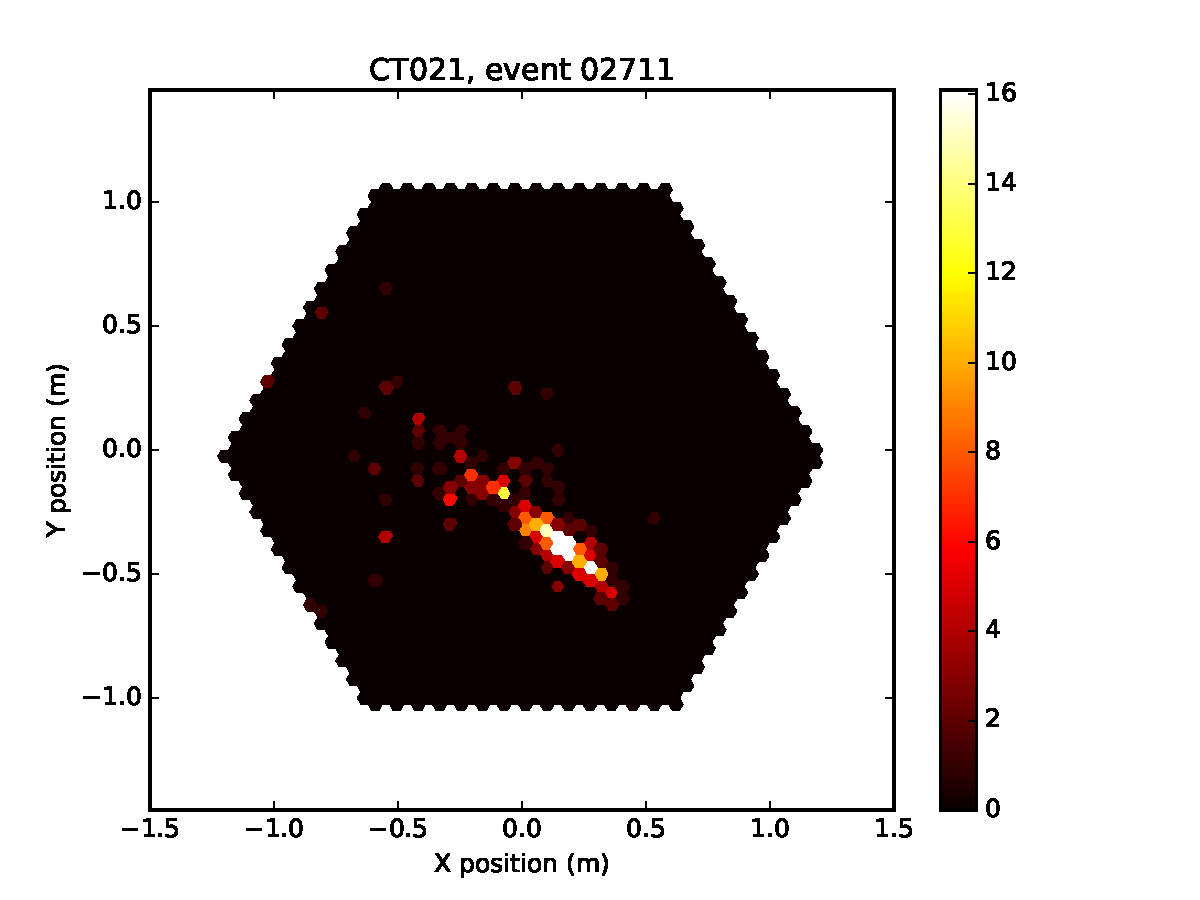
\includegraphics[trim=0 0 2cm 0,clip,width=\textwidth]{pics/img_pe}};
                    \draw[white,fill=white] (pic.south west) rectangle ($(pic.north west)!0.15!(pic.north east)$);
                    \draw[white,fill=white] (pic.north west) rectangle ($(pic.north east)!0.11!(pic.south east)$);
                    \draw[white,fill=white] (pic.south west) rectangle ($(pic.south east)!0.115!(pic.north east)$);
                    \foreach \x in {-1.5,-1,...,1.5}{
                        \node[scale=1.,anchor=north] at (\x*10mm + 21.7mm, 4.5mm) {$\x$};
                        \node[scale=1.,anchor=east]  at (7.mm,\x*10mm + 19.mm ) {$\x$};
                    }
                    \node[anchor=south east]           at ([xshift=-5mm,yshift=-2.5mm]pic.south east) {$x_\mathrm{pixel} / \si{m}$};
                    \node[anchor=north east,rotate=90] at ([xshift=-2mm,yshift=-5mm]pic.north west) {$y_\mathrm{pixel} / \si{m}$};
                \end{tikzpicture}
                
            \pause
            \column{.15\textwidth}
                \centering
                \vspace{.2cm}\ \\
                Stars, Clouds, \\
                Electronics etc.\\
                $\longrightarrow$\\
                \vspace{.7cm}
                \only<2>{
                    \ \\
                    \ \\
                    \ }
                \only<3->{
                    $\longleftarrow$\\
                    How to get back?
                }
            \column{.35\textwidth}
                \centering
                Detector Response
                \begin{tikzpicture}
                    \node[anchor=south west] (pic) at (0,0) {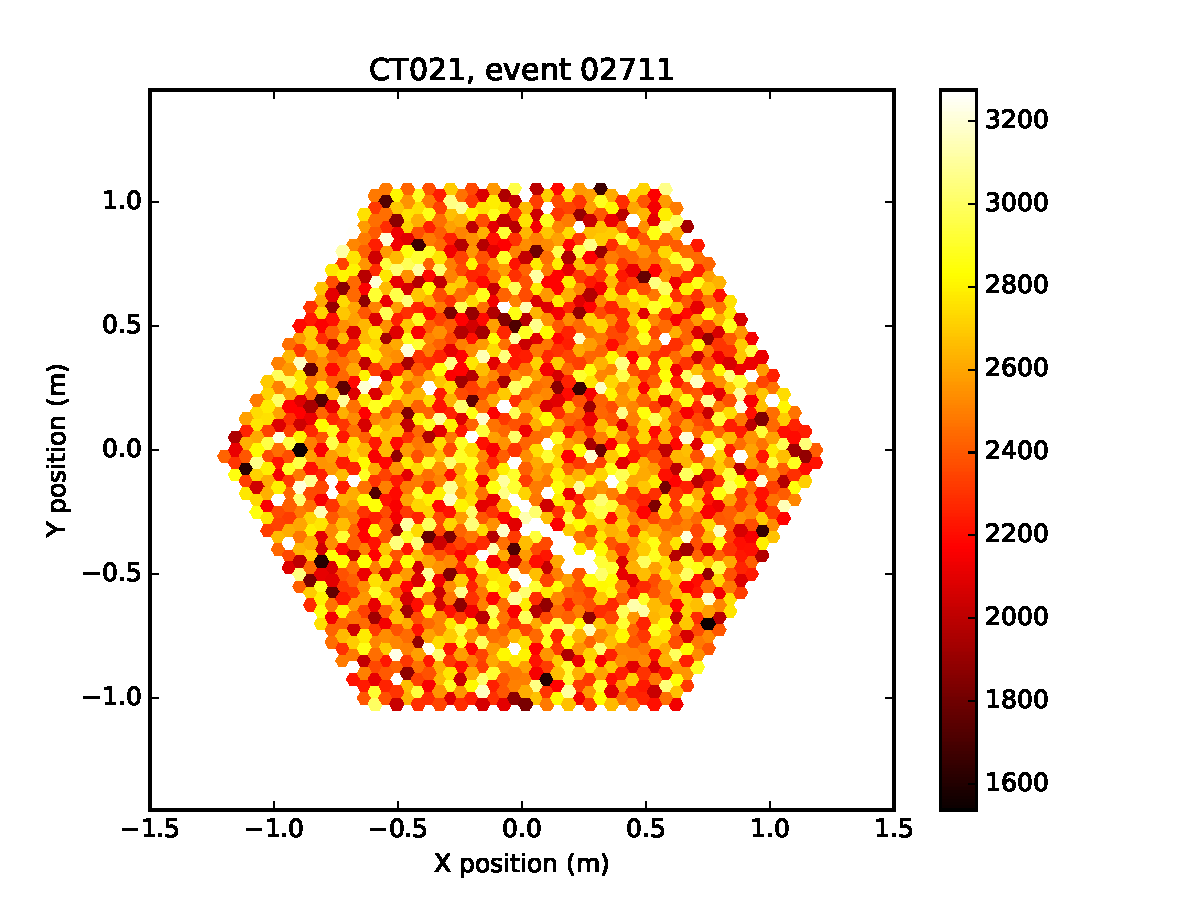
\includegraphics[trim=0 0 2cm 0,clip,width=\textwidth]{pics/img}};
                    \draw[white,fill=white] (pic.south west) rectangle ($(pic.north west)!0.15!(pic.north east)$);
                    \draw[white,fill=white] (pic.north west) rectangle ($(pic.north east)!0.11!(pic.south east)$);
                    \draw[white,fill=white] (pic.south west) rectangle ($(pic.south east)!0.115!(pic.north east)$);
                    \foreach \x in {-1.5,-1,...,1.5}{
                        \node[scale=1.,anchor=north] at (\x*10mm + 21.7mm, 4.5mm) {$\x$};
                        \node[scale=1.,anchor=east]  at (7mm,\x*10mm + 19.mm ) {$\x$};
                    }
                    \node[anchor=south east]           at ([xshift=-5mm,yshift=-2.5mm]pic.south east) {$x_\mathrm{pixel} / \si{m}$};
                    \node[anchor=north east,rotate=90] at ([xshift=-2mm,yshift=-5mm]pic.north west) {$y_\mathrm{pixel} / \si{m}$};
                \end{tikzpicture}
                
        \end{columns}
        \vspace{12pt}
        \pause
        \pause
        \begin{description}
            \item[] \hspace{-55pt}possible solutions:
            \item [Tail-Cuts] Used by H.E.S.S.: Cut away all pixels below a given threshold\\ -- possibly recover neighbouring pixels through second, lower threshold.
%             \medskip
            \item [Fourier Trans.] Decompose image into Fourier coefficients and cut in Fourier space.
%             \medskip
            \item [Wavelet Trans.] Decompose image into waveletes (in contrast to waves) and cut there.
        \end{description}
    
    \end{frame}


    \begin{frame}{Comparing Methods}
        \centering
        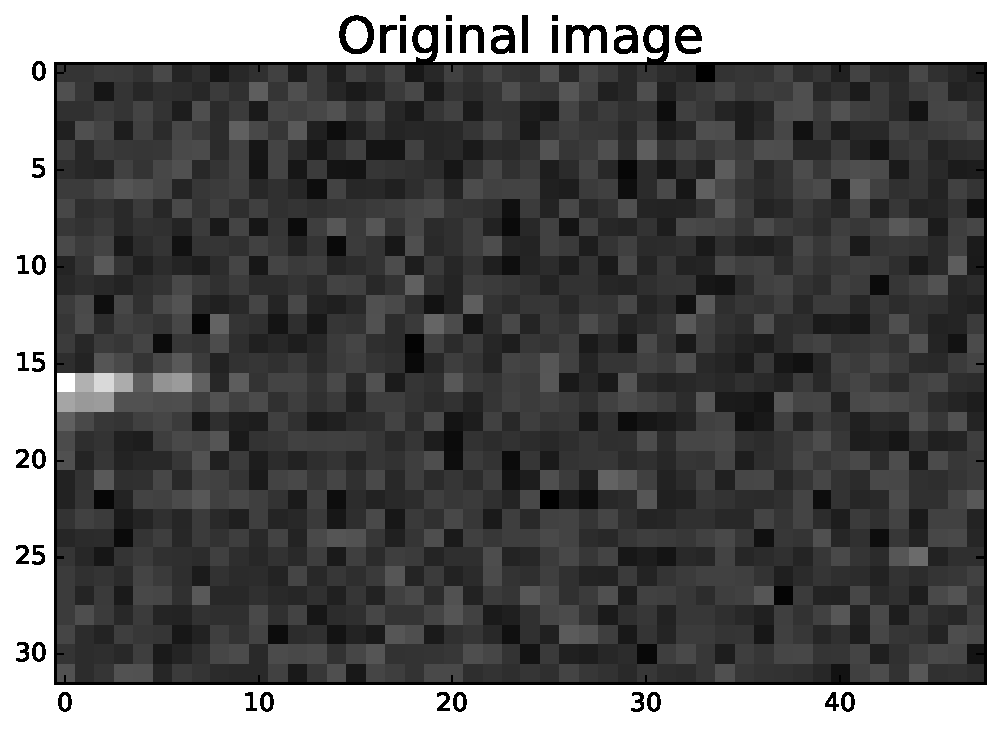
\includegraphics[width=.45\textwidth]{pics/CT066}
        \hspace{5mm}
        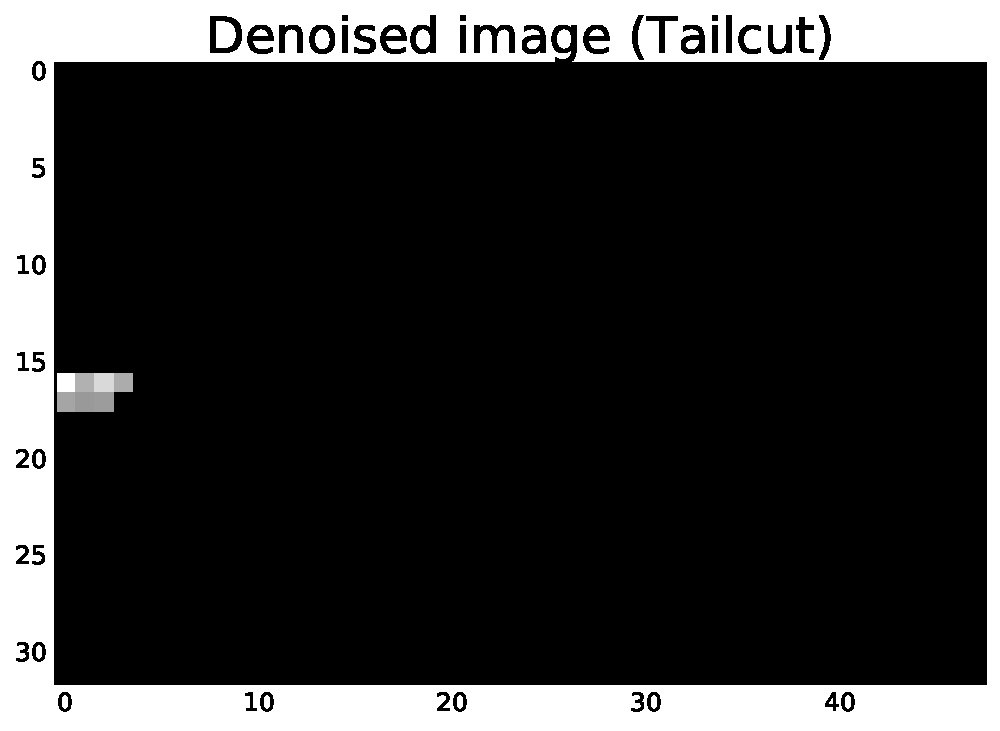
\includegraphics[width=.45\textwidth]{pics/CT066_tailcut_denoised}\\
        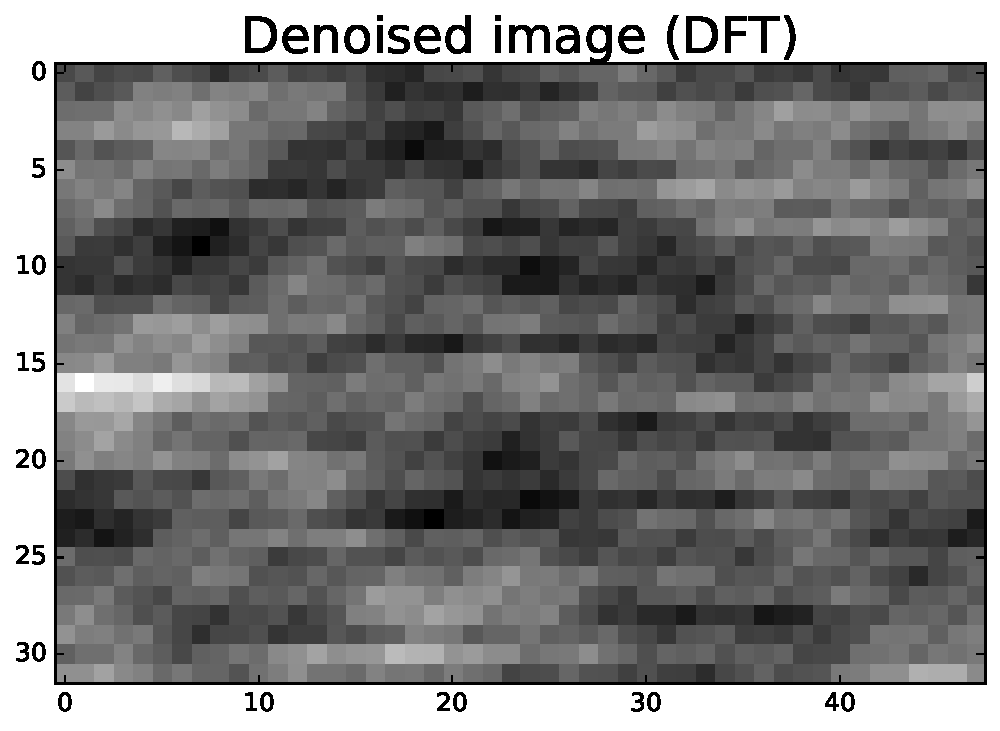
\includegraphics[width=.45\textwidth]{pics/CT066_dft_denoised}
        \hspace{5mm}
        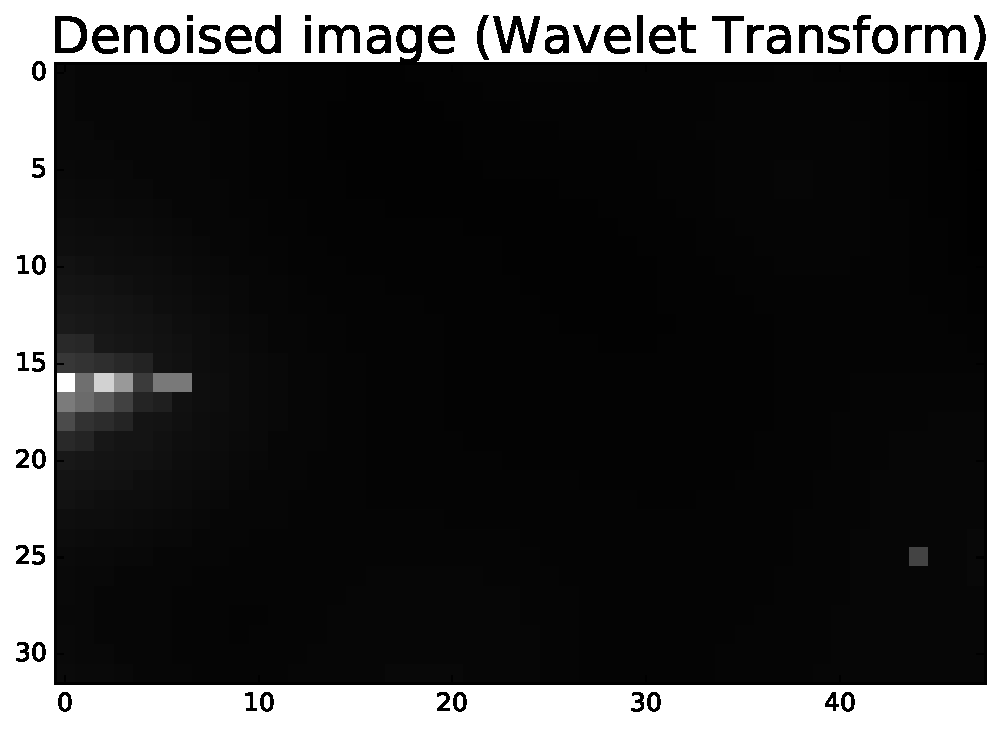
\includegraphics[width=.45\textwidth]{pics/CT066_wt_denoised}
        
    \end{frame}

    
    \begin{frame}{Shower Reconstruction}
        \begin{columns}
            \column{.6\textwidth}
                \begin{tikzpicture}
                \only<1>{
                    \node[anchor = center] (pic1) at (0,0) {
                        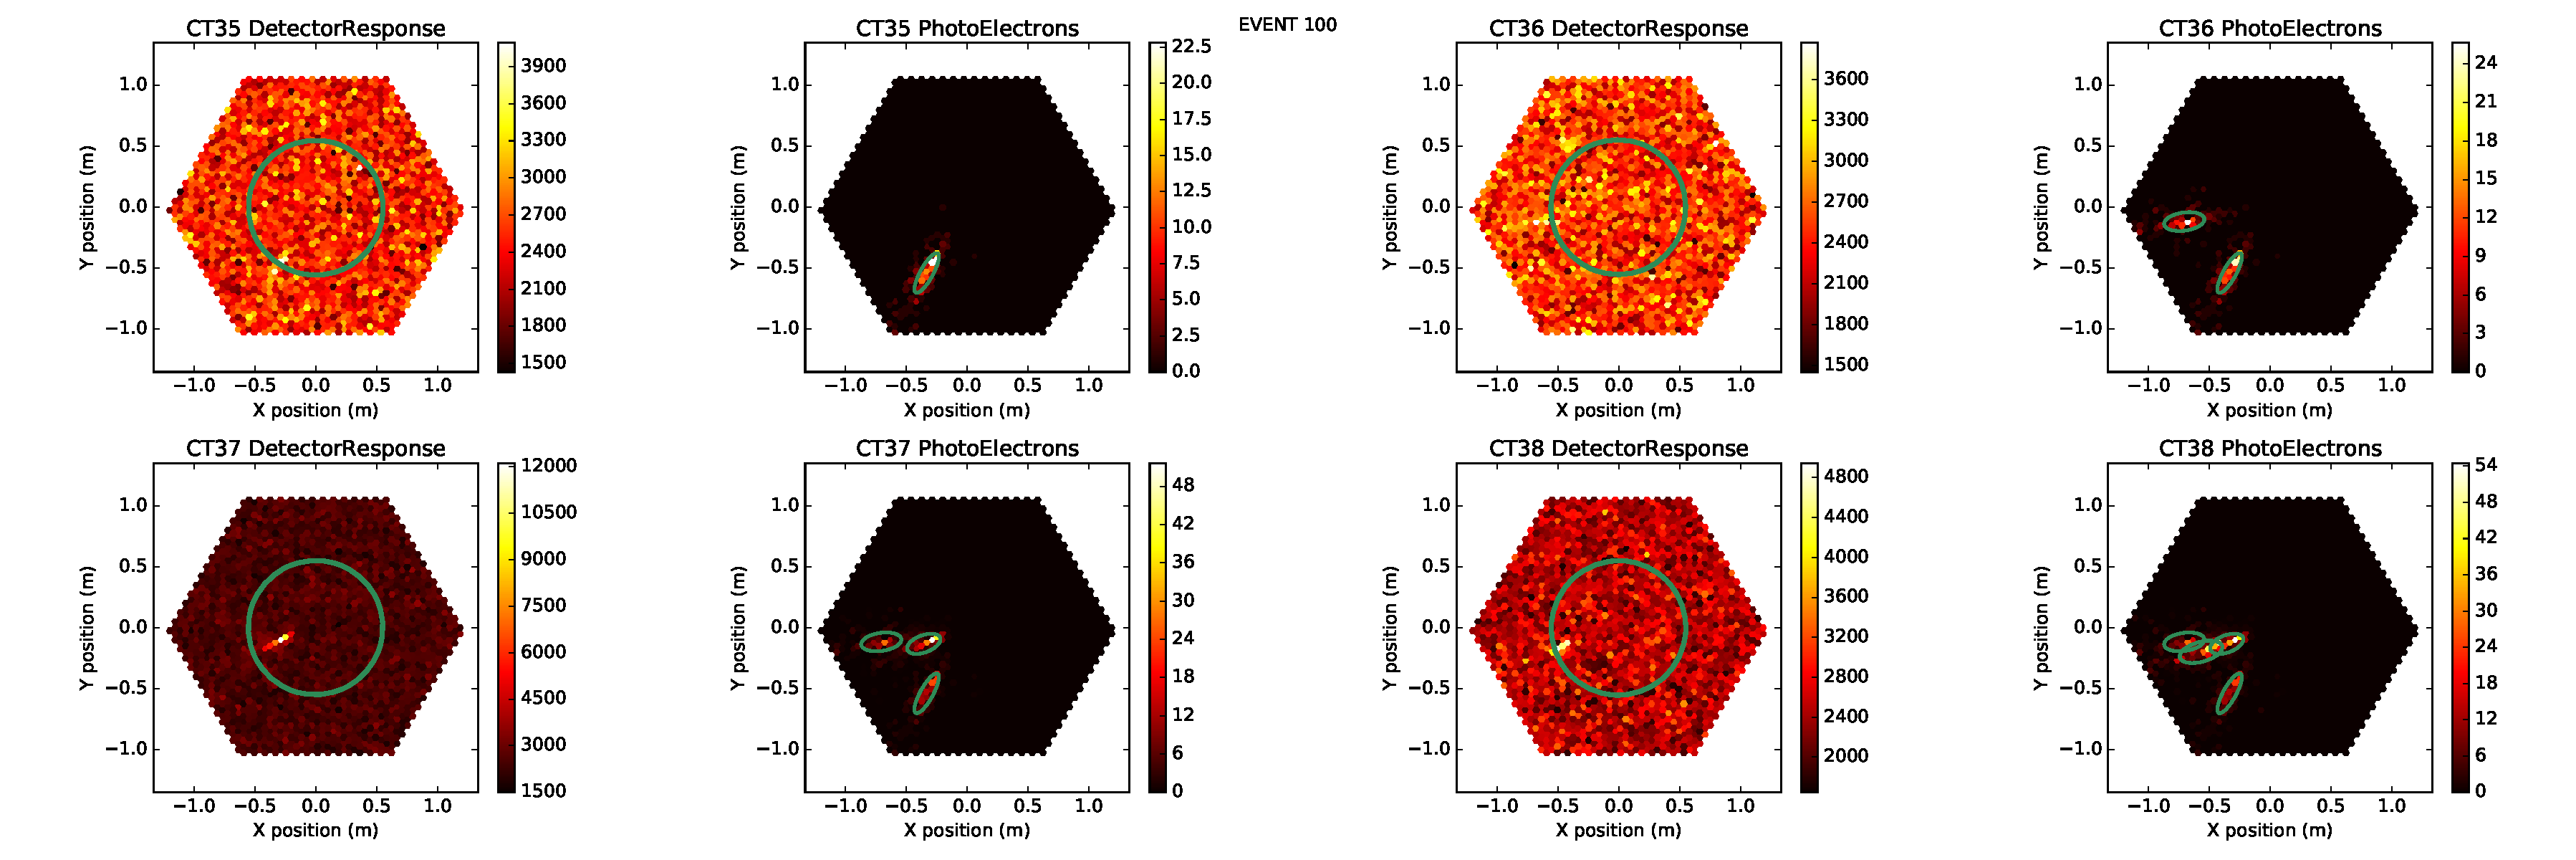
\includegraphics[trim=17cm 10cm 32cm .85cm,clip, width=\textwidth]{pics/hillas_overlay}
                    };
                }
                \only<2->{
                    \node[anchor = center] (pic1) at (0,0) {
                        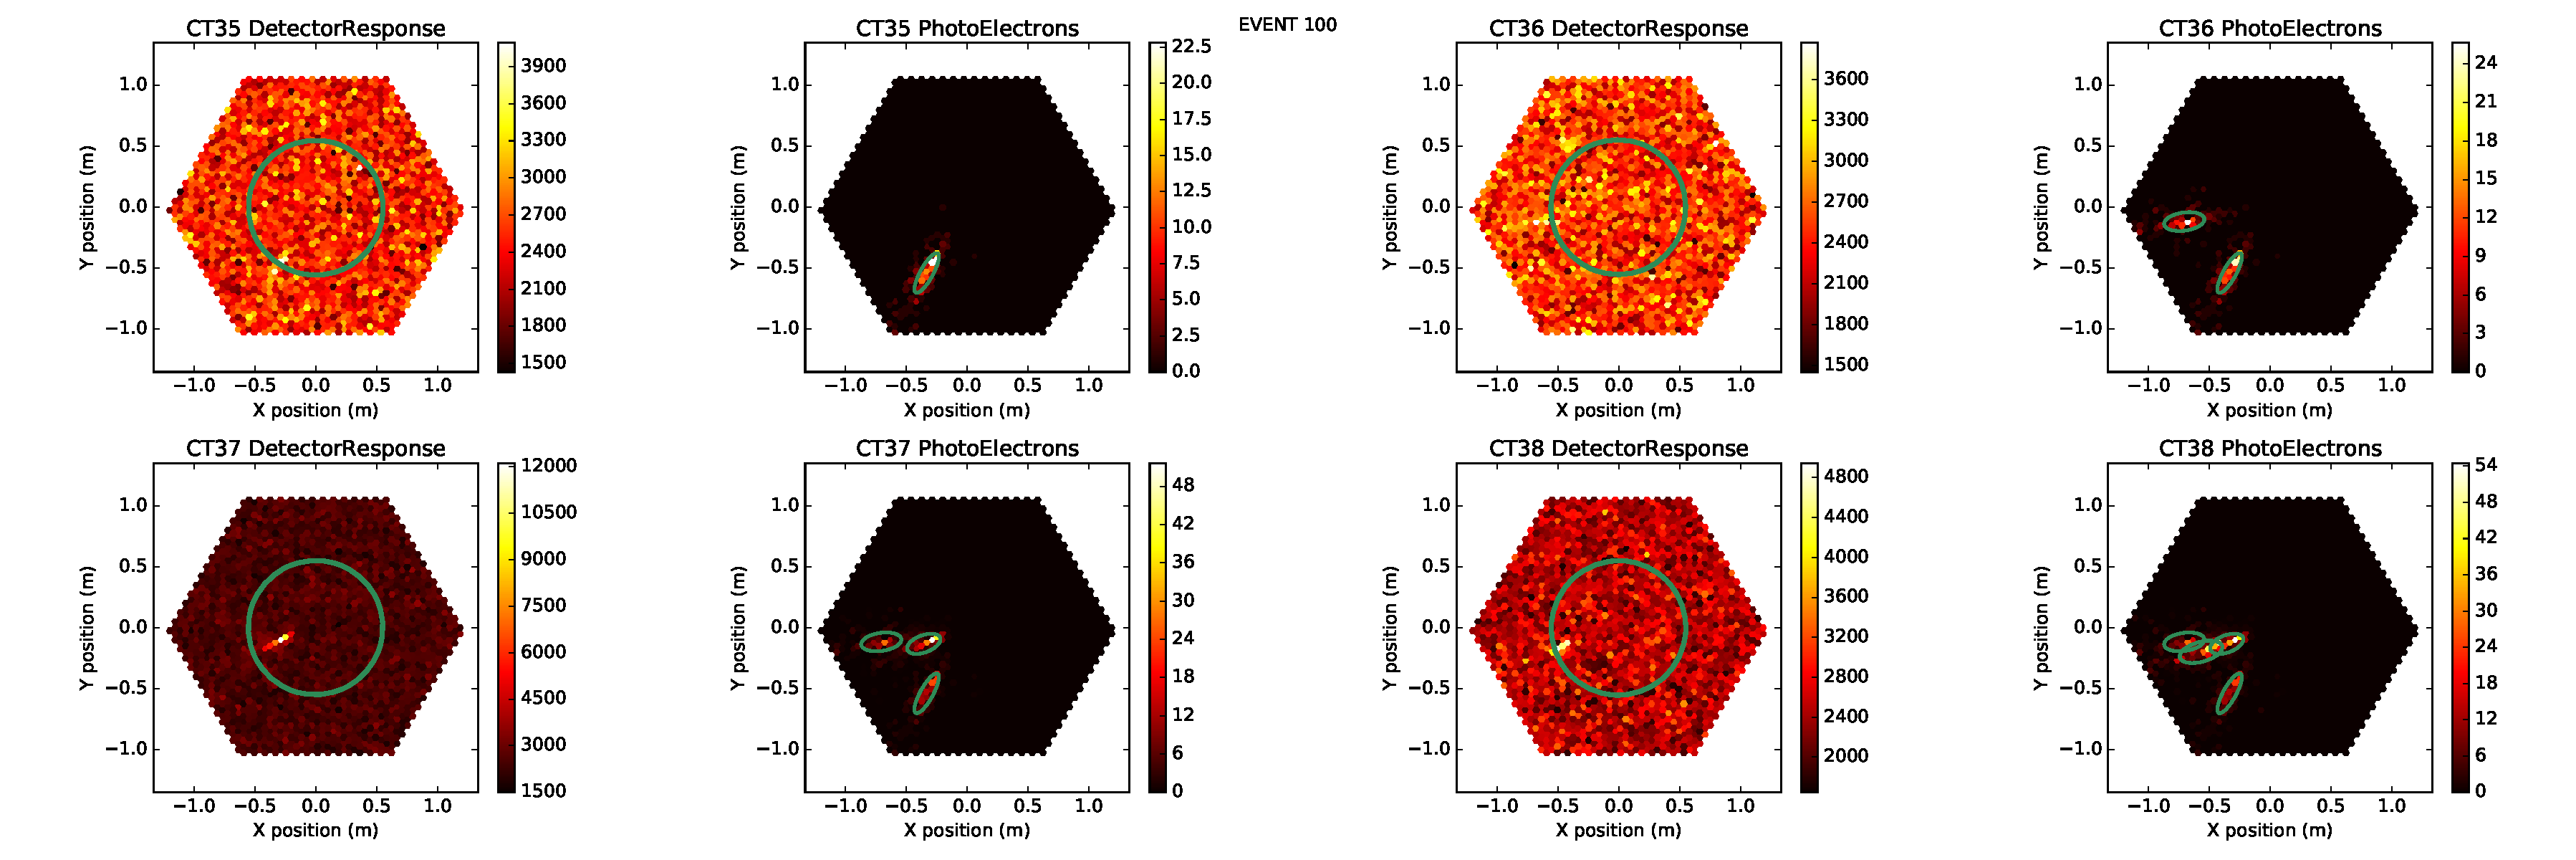
\includegraphics[trim=17cm .2cm 32cm 10.85cm,clip, width=\textwidth]{pics/hillas_overlay}
                    };
                }
                \only<3->{
                    \draw[line width=.4mm,green] (0,5.8mm) -- +(240.5:2cm);
                    \draw[line width=.4mm,green] (0,4.2mm) -- +(200:2cm);
                    \draw[line width=.4mm,green] (0,3.9mm) -- +(188:2cm);
                }
                \end{tikzpicture}
            \column{.4\textwidth}
                \begin{itemize}
                    \item construct an ellipsis with moments of the shower image:\\
                    \emph{Hillas Parametrisation}
                    \pause
                    \item combine images from different cameras
                    \pause
                    \item intersection of their ellipsis axes is
                        the shower origin
                \end{itemize}

        \end{columns}

    \end{frame}

    
    
    \begin{frame}{Shower Reconstruction -- Performance}
                 {angle between reconstructed and simulated direction}
        \setlength{\figureheight}{6cm}
        \begin{columns}
            \column{.5\textwidth}
                \centering
                tail cuts\\
                % This file was created by matplotlib2tikz v0.5.12.
\begin{tikzpicture}

\definecolor{color0}{rgb}{0.75,0.75,0}

\begin{axis}[
xlabel={Number of Telescopes},
ylabel={$\log(\xi /  \si{\degree})$},
ytick={-3,-2,-1,0,1,2},
xmin=1, xmax=10,
ymin=-4, ymax=3,
axis on top,
width=\figurewidth,
height=\figureheight,
xmajorgrids,
ymajorgrids
]
\path [draw=black, fill=color0, opacity=0.3] (axis cs:2.00256683758479,-2.29633559755855)
--(axis cs:1.99743316241521,-2.29633559755855)
--(axis cs:1.99640725639552,-2.22428989474736)
--(axis cs:1.99540769057537,-2.15224419193617)
--(axis cs:1.99445530795193,-2.08019848912497)
--(axis cs:1.99337857835994,-2.00815278631378)
--(axis cs:1.99180715531967,-1.93610708350259)
--(axis cs:1.98927286666639,-1.8640613806914)
--(axis cs:1.98528355696037,-1.79201567788021)
--(axis cs:1.97924434026484,-1.71996997506902)
--(axis cs:1.97040965204055,-1.64792427225782)
--(axis cs:1.95822756535057,-1.57587856944663)
--(axis cs:1.94296709250862,-1.50383286663544)
--(axis cs:1.92588061636953,-1.43178716382425)
--(axis cs:1.90838467093818,-1.35974146101306)
--(axis cs:1.89079186676115,-1.28769575820187)
--(axis cs:1.87188861717247,-1.21565005539067)
--(axis cs:1.85019000034566,-1.14360435257948)
--(axis cs:1.82601719097069,-1.07155864976829)
--(axis cs:1.80220922362868,-0.9995129469571)
--(axis cs:1.78224179914077,-0.927467244145908)
--(axis cs:1.76724653829139,-0.855421541334716)
--(axis cs:1.75493080994732,-0.783375838523525)
--(axis cs:1.74173014018818,-0.711330135712333)
--(axis cs:1.72615078423247,-0.639284432901141)
--(axis cs:1.70972042872687,-0.56723873008995)
--(axis cs:1.69440794186445,-0.495193027278758)
--(axis cs:1.67975722855011,-0.423147324467566)
--(axis cs:1.66376396003841,-0.351101621656374)
--(axis cs:1.64659265603523,-0.279055918845183)
--(axis cs:1.63207410543465,-0.207010216033991)
--(axis cs:1.625,-0.134964513222799)
--(axis cs:1.62790017468226,-0.0629188104116079)
--(axis cs:1.64068622742175,0.00912689239958375)
--(axis cs:1.66201122314714,0.0811725952107754)
--(axis cs:1.69001965247035,0.153218298021967)
--(axis cs:1.72239246060194,0.225264000833159)
--(axis cs:1.7564621698082,0.29730970364435)
--(axis cs:1.78957713574594,0.369355406455542)
--(axis cs:1.81973853591332,0.441401109266734)
--(axis cs:1.84616881753293,0.513446812077925)
--(axis cs:1.86908359184927,0.585492514889117)
--(axis cs:1.88885955942192,0.657538217700309)
--(axis cs:1.90566307042711,0.7295839205115)
--(axis cs:1.91976569513995,0.801629623322692)
--(axis cs:1.93173321084589,0.873675326133884)
--(axis cs:1.9420883292892,0.945721028945075)
--(axis cs:1.95095123233244,1.01776673175627)
--(axis cs:1.95814637478395,1.08981243456746)
--(axis cs:1.96360015059538,1.16185813737865)
--(axis cs:1.96756974754273,1.23390384018984)
--(axis cs:1.97055978569574,1.30594954300103)
--(axis cs:1.9731178900109,1.37799524581223)
--(axis cs:1.97567894116766,1.45004094862342)
--(axis cs:1.97845521398178,1.52208665143461)
--(axis cs:1.98135991384281,1.5941323542458)
--(axis cs:1.98408557616605,1.66617805705699)
--(axis cs:1.98640391118077,1.73822375986818)
--(axis cs:1.98843349285385,1.81026946267938)
--(axis cs:1.99053260715492,1.88231516549057)
--(axis cs:1.99289672928395,1.95436086830176)
--(axis cs:2.00710327071605,1.95436086830176)
--(axis cs:2.00710327071605,1.95436086830176)
--(axis cs:2.00946739284508,1.88231516549057)
--(axis cs:2.01156650714615,1.81026946267938)
--(axis cs:2.01359608881923,1.73822375986818)
--(axis cs:2.01591442383395,1.66617805705699)
--(axis cs:2.01864008615719,1.5941323542458)
--(axis cs:2.02154478601822,1.52208665143461)
--(axis cs:2.02432105883234,1.45004094862342)
--(axis cs:2.0268821099891,1.37799524581223)
--(axis cs:2.02944021430426,1.30594954300103)
--(axis cs:2.03243025245727,1.23390384018984)
--(axis cs:2.03639984940462,1.16185813737865)
--(axis cs:2.04185362521605,1.08981243456746)
--(axis cs:2.04904876766756,1.01776673175627)
--(axis cs:2.0579116707108,0.945721028945075)
--(axis cs:2.06826678915411,0.873675326133884)
--(axis cs:2.08023430486005,0.801629623322692)
--(axis cs:2.09433692957289,0.7295839205115)
--(axis cs:2.11114044057808,0.657538217700309)
--(axis cs:2.13091640815073,0.585492514889117)
--(axis cs:2.15383118246707,0.513446812077925)
--(axis cs:2.18026146408668,0.441401109266734)
--(axis cs:2.21042286425406,0.369355406455542)
--(axis cs:2.2435378301918,0.29730970364435)
--(axis cs:2.27760753939806,0.225264000833159)
--(axis cs:2.30998034752965,0.153218298021967)
--(axis cs:2.33798877685286,0.0811725952107754)
--(axis cs:2.35931377257825,0.00912689239958375)
--(axis cs:2.37209982531774,-0.0629188104116079)
--(axis cs:2.375,-0.134964513222799)
--(axis cs:2.36792589456535,-0.207010216033991)
--(axis cs:2.35340734396477,-0.279055918845183)
--(axis cs:2.33623603996159,-0.351101621656374)
--(axis cs:2.32024277144989,-0.423147324467566)
--(axis cs:2.30559205813555,-0.495193027278758)
--(axis cs:2.29027957127313,-0.56723873008995)
--(axis cs:2.27384921576753,-0.639284432901141)
--(axis cs:2.25826985981182,-0.711330135712333)
--(axis cs:2.24506919005268,-0.783375838523525)
--(axis cs:2.23275346170861,-0.855421541334716)
--(axis cs:2.21775820085923,-0.927467244145908)
--(axis cs:2.19779077637132,-0.9995129469571)
--(axis cs:2.17398280902931,-1.07155864976829)
--(axis cs:2.14980999965434,-1.14360435257948)
--(axis cs:2.12811138282753,-1.21565005539067)
--(axis cs:2.10920813323885,-1.28769575820187)
--(axis cs:2.09161532906182,-1.35974146101306)
--(axis cs:2.07411938363047,-1.43178716382425)
--(axis cs:2.05703290749138,-1.50383286663544)
--(axis cs:2.04177243464943,-1.57587856944663)
--(axis cs:2.02959034795945,-1.64792427225782)
--(axis cs:2.02075565973516,-1.71996997506902)
--(axis cs:2.01471644303963,-1.79201567788021)
--(axis cs:2.01072713333361,-1.8640613806914)
--(axis cs:2.00819284468033,-1.93610708350259)
--(axis cs:2.00662142164005,-2.00815278631378)
--(axis cs:2.00554469204807,-2.08019848912497)
--(axis cs:2.00459230942463,-2.15224419193617)
--(axis cs:2.00359274360448,-2.22428989474736)
--(axis cs:2.00256683758479,-2.29633559755855)
--cycle;

\path [draw=black, fill=color0, opacity=0.3] (axis cs:3.00513451497069,-2.07853637960157)
--(axis cs:2.99486548502931,-2.07853637960157)
--(axis cs:2.99375649843291,-2.01663787725097)
--(axis cs:2.99254227935711,-1.95473937490038)
--(axis cs:2.99089224613199,-1.89284087254978)
--(axis cs:2.98859598580448,-1.83094237019919)
--(axis cs:2.98565674898377,-1.76904386784859)
--(axis cs:2.98198632863425,-1.707145365498)
--(axis cs:2.97688131159589,-1.64524686314741)
--(axis cs:2.96885602120727,-1.58334836079681)
--(axis cs:2.95625485935377,-1.52144985844622)
--(axis cs:2.93833842708114,-1.45955135609562)
--(axis cs:2.91596628196206,-1.39765285374503)
--(axis cs:2.89130133761507,-1.33575435139443)
--(axis cs:2.8668708349244,-1.27385584904384)
--(axis cs:2.84481237172814,-1.21195734669324)
--(axis cs:2.82667768923743,-1.15005884434265)
--(axis cs:2.8134110439832,-1.08816034199205)
--(axis cs:2.80506558867056,-1.02626183964146)
--(axis cs:2.80045738259109,-0.964363337290865)
--(axis cs:2.79727865176568,-0.902464834940271)
--(axis cs:2.79273932112863,-0.840566332589676)
--(axis cs:2.78434954158749,-0.778667830239082)
--(axis cs:2.77064082882291,-0.716769327888487)
--(axis cs:2.75184309052337,-0.654870825537893)
--(axis cs:2.73010946801351,-0.592972323187298)
--(axis cs:2.70857978881438,-0.531073820836704)
--(axis cs:2.68950667392305,-0.469175318486109)
--(axis cs:2.67302251615906,-0.407276816135514)
--(axis cs:2.65787566352578,-0.34537831378492)
--(axis cs:2.64350934183431,-0.283479811434325)
--(axis cs:2.63148386747923,-0.221581309083731)
--(axis cs:2.625,-0.159682806733136)
--(axis cs:2.62711120016355,-0.0977843043825417)
--(axis cs:2.63914919347509,-0.035885802031947)
--(axis cs:2.66032924538226,0.0260127003186472)
--(axis cs:2.68838831480023,0.0879112026692419)
--(axis cs:2.72053915062453,0.149809705019837)
--(axis cs:2.75418344961808,0.211708207370431)
--(axis cs:2.78724046034635,0.273606709721026)
--(axis cs:2.81824231113197,0.33550521207162)
--(axis cs:2.84640128660047,0.397403714422215)
--(axis cs:2.87165564860528,0.459302216772809)
--(axis cs:2.89448678648012,0.521200719123404)
--(axis cs:2.91541322528131,0.583099221473999)
--(axis cs:2.93444295140564,0.644997723824593)
--(axis cs:2.95094751115613,0.706896226175187)
--(axis cs:2.96413005498217,0.768794728525782)
--(axis cs:2.97371693482196,0.830693230876376)
--(axis cs:2.98024963063963,0.892591733226971)
--(axis cs:2.98473114338656,0.954490235577566)
--(axis cs:2.98803090383303,1.01638873792816)
--(axis cs:2.99061460720666,1.07828724027875)
--(axis cs:2.99268464925366,1.14018574262935)
--(axis cs:2.99437651076496,1.20208424497994)
--(axis cs:2.99577075630783,1.26398274733054)
--(axis cs:2.996835132183,1.32588124968113)
--(axis cs:2.99748298656104,1.38777975203173)
--(axis cs:2.99772403818609,1.44967825438232)
--(axis cs:2.99773886290872,1.51157675673292)
--(axis cs:2.9977891490517,1.57347525908351)
--(axis cs:3.0022108509483,1.57347525908351)
--(axis cs:3.0022108509483,1.57347525908351)
--(axis cs:3.00226113709128,1.51157675673292)
--(axis cs:3.00227596181391,1.44967825438232)
--(axis cs:3.00251701343896,1.38777975203173)
--(axis cs:3.003164867817,1.32588124968113)
--(axis cs:3.00422924369217,1.26398274733054)
--(axis cs:3.00562348923504,1.20208424497994)
--(axis cs:3.00731535074634,1.14018574262935)
--(axis cs:3.00938539279334,1.07828724027875)
--(axis cs:3.01196909616697,1.01638873792816)
--(axis cs:3.01526885661344,0.954490235577566)
--(axis cs:3.01975036936037,0.892591733226971)
--(axis cs:3.02628306517804,0.830693230876376)
--(axis cs:3.03586994501783,0.768794728525782)
--(axis cs:3.04905248884387,0.706896226175187)
--(axis cs:3.06555704859436,0.644997723824593)
--(axis cs:3.08458677471869,0.583099221473999)
--(axis cs:3.10551321351988,0.521200719123404)
--(axis cs:3.12834435139472,0.459302216772809)
--(axis cs:3.15359871339953,0.397403714422215)
--(axis cs:3.18175768886803,0.33550521207162)
--(axis cs:3.21275953965365,0.273606709721026)
--(axis cs:3.24581655038192,0.211708207370431)
--(axis cs:3.27946084937547,0.149809705019837)
--(axis cs:3.31161168519977,0.0879112026692419)
--(axis cs:3.33967075461774,0.0260127003186472)
--(axis cs:3.36085080652491,-0.035885802031947)
--(axis cs:3.37288879983645,-0.0977843043825417)
--(axis cs:3.375,-0.159682806733136)
--(axis cs:3.36851613252077,-0.221581309083731)
--(axis cs:3.35649065816569,-0.283479811434325)
--(axis cs:3.34212433647422,-0.34537831378492)
--(axis cs:3.32697748384094,-0.407276816135514)
--(axis cs:3.31049332607695,-0.469175318486109)
--(axis cs:3.29142021118562,-0.531073820836704)
--(axis cs:3.26989053198649,-0.592972323187298)
--(axis cs:3.24815690947663,-0.654870825537893)
--(axis cs:3.22935917117709,-0.716769327888487)
--(axis cs:3.21565045841251,-0.778667830239082)
--(axis cs:3.20726067887137,-0.840566332589676)
--(axis cs:3.20272134823432,-0.902464834940271)
--(axis cs:3.19954261740891,-0.964363337290865)
--(axis cs:3.19493441132944,-1.02626183964146)
--(axis cs:3.1865889560168,-1.08816034199205)
--(axis cs:3.17332231076257,-1.15005884434265)
--(axis cs:3.15518762827186,-1.21195734669324)
--(axis cs:3.1331291650756,-1.27385584904384)
--(axis cs:3.10869866238493,-1.33575435139443)
--(axis cs:3.08403371803794,-1.39765285374503)
--(axis cs:3.06166157291886,-1.45955135609562)
--(axis cs:3.04374514064623,-1.52144985844622)
--(axis cs:3.03114397879273,-1.58334836079681)
--(axis cs:3.02311868840411,-1.64524686314741)
--(axis cs:3.01801367136575,-1.707145365498)
--(axis cs:3.01434325101623,-1.76904386784859)
--(axis cs:3.01140401419552,-1.83094237019919)
--(axis cs:3.00910775386801,-1.89284087254978)
--(axis cs:3.00745772064289,-1.95473937490038)
--(axis cs:3.00624350156709,-2.01663787725097)
--(axis cs:3.00513451497069,-2.07853637960157)
--cycle;

\path [draw=black, fill=color0, opacity=0.3] (axis cs:4.0025841756911,-2.25643057170547)
--(axis cs:3.9974158243089,-2.25643057170547)
--(axis cs:3.99756197882787,-2.20277953840782)
--(axis cs:3.99793030621852,-2.14912850511017)
--(axis cs:3.99828006879116,-2.09547747181252)
--(axis cs:3.99826963944574,-2.04182643851487)
--(axis cs:3.99748749072563,-1.98817540521721)
--(axis cs:3.99548381468315,-1.93452437191956)
--(axis cs:3.99186274734125,-1.88087333862191)
--(axis cs:3.98645741564895,-1.82722230532426)
--(axis cs:3.97948773122488,-1.77357127202661)
--(axis cs:3.97152011916648,-1.71992023872896)
--(axis cs:3.96315198258743,-1.6662692054313)
--(axis cs:3.95460591294676,-1.61261817213365)
--(axis cs:3.9455927426056,-1.558967138836)
--(axis cs:3.93564615652925,-1.50531610553835)
--(axis cs:3.92471709185356,-1.4516650722407)
--(axis cs:3.91352906576525,-1.39801403894305)
--(axis cs:3.90334377846001,-1.34436300564539)
--(axis cs:3.89525561771568,-1.29071197234774)
--(axis cs:3.88950601483256,-1.23706093905009)
--(axis cs:3.88528512003435,-1.18340990575244)
--(axis cs:3.88112826446603,-1.12975887245479)
--(axis cs:3.87561736957919,-1.07610783915714)
--(axis cs:3.8679454060725,-1.02245680585948)
--(axis cs:3.85806919952252,-0.968805772561833)
--(axis cs:3.84647947312808,-0.915154739264181)
--(axis cs:3.83378710727768,-0.861503705966529)
--(axis cs:3.8202941674408,-0.807852672668878)
--(axis cs:3.80567660953996,-0.754201639371226)
--(axis cs:3.78898091328662,-0.700550606073574)
--(axis cs:3.76914021845422,-0.646899572775923)
--(axis cs:3.74588880867325,-0.593248539478271)
--(axis cs:3.72045458277519,-0.53959750618062)
--(axis cs:3.69531949336018,-0.485946472882968)
--(axis cs:3.67300968394038,-0.432295439585316)
--(axis cs:3.65483234170533,-0.378644406287665)
--(axis cs:3.64071736948472,-0.324993372990013)
--(axis cs:3.63041391542403,-0.271342339692361)
--(axis cs:3.625,-0.217691306394709)
--(axis cs:3.62725183286872,-0.164040273097058)
--(axis cs:3.64032514803146,-0.110389239799406)
--(axis cs:3.66560984856872,-0.0567382065017545)
--(axis cs:3.70131971182891,-0.0030871732041029)
--(axis cs:3.74284621801978,0.0505638600935487)
--(axis cs:3.78463571969176,0.1042148933912)
--(axis cs:3.82236288776435,0.157865926688852)
--(axis cs:3.85416145068841,0.211516959986504)
--(axis cs:3.88046748707916,0.265167993284155)
--(axis cs:3.90289453045766,0.318819026581807)
--(axis cs:3.92294233880996,0.372470059879459)
--(axis cs:3.94121174181999,0.42612109317711)
--(axis cs:3.95738484544086,0.479772126474762)
--(axis cs:3.97076590115089,0.533423159772414)
--(axis cs:3.98090143515836,0.587074193070065)
--(axis cs:3.98787720897325,0.640725226367717)
--(axis cs:3.99222716974073,0.694376259665368)
--(axis cs:3.99466994713779,0.74802729296302)
--(axis cs:3.99590150926267,0.801678326260672)
--(axis cs:3.99650483270042,0.855329359558323)
--(axis cs:3.99691267488984,0.908980392855975)
--(axis cs:4.00308732511016,0.908980392855975)
--(axis cs:4.00308732511016,0.908980392855975)
--(axis cs:4.00349516729958,0.855329359558323)
--(axis cs:4.00409849073733,0.801678326260672)
--(axis cs:4.00533005286221,0.74802729296302)
--(axis cs:4.00777283025927,0.694376259665368)
--(axis cs:4.01212279102675,0.640725226367717)
--(axis cs:4.01909856484164,0.587074193070065)
--(axis cs:4.02923409884911,0.533423159772414)
--(axis cs:4.04261515455914,0.479772126474762)
--(axis cs:4.05878825818001,0.42612109317711)
--(axis cs:4.07705766119004,0.372470059879459)
--(axis cs:4.09710546954234,0.318819026581807)
--(axis cs:4.11953251292084,0.265167993284155)
--(axis cs:4.14583854931159,0.211516959986504)
--(axis cs:4.17763711223565,0.157865926688852)
--(axis cs:4.21536428030824,0.1042148933912)
--(axis cs:4.25715378198022,0.0505638600935487)
--(axis cs:4.29868028817109,-0.0030871732041029)
--(axis cs:4.33439015143128,-0.0567382065017545)
--(axis cs:4.35967485196854,-0.110389239799406)
--(axis cs:4.37274816713129,-0.164040273097058)
--(axis cs:4.375,-0.217691306394709)
--(axis cs:4.36958608457597,-0.271342339692361)
--(axis cs:4.35928263051528,-0.324993372990013)
--(axis cs:4.34516765829467,-0.378644406287665)
--(axis cs:4.32699031605962,-0.432295439585316)
--(axis cs:4.30468050663982,-0.485946472882968)
--(axis cs:4.27954541722481,-0.53959750618062)
--(axis cs:4.25411119132675,-0.593248539478271)
--(axis cs:4.23085978154578,-0.646899572775923)
--(axis cs:4.21101908671338,-0.700550606073574)
--(axis cs:4.19432339046004,-0.754201639371226)
--(axis cs:4.1797058325592,-0.807852672668878)
--(axis cs:4.16621289272232,-0.861503705966529)
--(axis cs:4.15352052687192,-0.915154739264181)
--(axis cs:4.14193080047748,-0.968805772561833)
--(axis cs:4.1320545939275,-1.02245680585948)
--(axis cs:4.12438263042081,-1.07610783915714)
--(axis cs:4.11887173553397,-1.12975887245479)
--(axis cs:4.11471487996565,-1.18340990575244)
--(axis cs:4.11049398516744,-1.23706093905009)
--(axis cs:4.10474438228432,-1.29071197234774)
--(axis cs:4.09665622153999,-1.34436300564539)
--(axis cs:4.08647093423475,-1.39801403894305)
--(axis cs:4.07528290814644,-1.4516650722407)
--(axis cs:4.06435384347075,-1.50531610553835)
--(axis cs:4.0544072573944,-1.558967138836)
--(axis cs:4.04539408705324,-1.61261817213365)
--(axis cs:4.03684801741257,-1.6662692054313)
--(axis cs:4.02847988083352,-1.71992023872896)
--(axis cs:4.02051226877512,-1.77357127202661)
--(axis cs:4.01354258435105,-1.82722230532426)
--(axis cs:4.00813725265875,-1.88087333862191)
--(axis cs:4.00451618531685,-1.93452437191956)
--(axis cs:4.00251250927437,-1.98817540521721)
--(axis cs:4.00173036055426,-2.04182643851487)
--(axis cs:4.00171993120884,-2.09547747181252)
--(axis cs:4.00206969378148,-2.14912850511017)
--(axis cs:4.00243802117213,-2.20277953840782)
--(axis cs:4.0025841756911,-2.25643057170547)
--cycle;

\path [draw=black, fill=color0, opacity=0.3] (axis cs:5.00732762972231,-2.18063678478164)
--(axis cs:4.99267237027769,-2.18063678478164)
--(axis cs:4.99154986134253,-2.12926521801216)
--(axis cs:4.99029420663654,-2.07789365124269)
--(axis cs:4.98868194310701,-2.02652208447321)
--(axis cs:4.98649274246226,-1.97515051770374)
--(axis cs:4.98358171788043,-1.92377895093426)
--(axis cs:4.97992125573114,-1.87240738416478)
--(axis cs:4.97559049479516,-1.82103581739531)
--(axis cs:4.97070350451579,-1.76966425062583)
--(axis cs:4.96529249752914,-1.71829268385636)
--(axis cs:4.95919881986749,-1.66692111708688)
--(axis cs:4.95204441868657,-1.6155495503174)
--(axis cs:4.94332648071134,-1.56417798354793)
--(axis cs:4.93260367836178,-1.51280641677845)
--(axis cs:4.91968098754902,-1.46143485000898)
--(axis cs:4.90470775856357,-1.4100632832395)
--(axis cs:4.88817083314654,-1.35869171647003)
--(axis cs:4.87081923466629,-1.30732014970055)
--(axis cs:4.85354737644376,-1.25594858293107)
--(axis cs:4.83722238657159,-1.2045770161616)
--(axis cs:4.82244665428178,-1.15320544939212)
--(axis cs:4.80932194673458,-1.10183388262265)
--(axis cs:4.79735333166936,-1.05046231585317)
--(axis cs:4.78560535274113,-0.999090749083694)
--(axis cs:4.7730882817455,-0.947719182314218)
--(axis cs:4.7591994246026,-0.896347615544743)
--(axis cs:4.74398714631142,-0.844976048775267)
--(axis cs:4.72809023636779,-0.793604482005791)
--(axis cs:4.71238461603889,-0.742232915236315)
--(axis cs:4.69753806686451,-0.690861348466839)
--(axis cs:4.68373228896654,-0.639489781697363)
--(axis cs:4.67072100269276,-0.588118214927887)
--(axis cs:4.65819880558673,-0.536746648158412)
--(axis cs:4.64626985366229,-0.485375081388936)
--(axis cs:4.63574255628843,-0.43400351461946)
--(axis cs:4.62807622041743,-0.382631947849984)
--(axis cs:4.625,-0.331260381080508)
--(axis cs:4.62798742275007,-0.279888814311032)
--(axis cs:4.63781419255135,-0.228517247541556)
--(axis cs:4.65435933316093,-0.17714568077208)
--(axis cs:4.67669454161334,-0.125774114002605)
--(axis cs:4.70339804278747,-0.0744025472331287)
--(axis cs:4.73295149050141,-0.0230309804636528)
--(axis cs:4.76405225642605,0.028340586305823)
--(axis cs:4.79572169056675,0.0797121530752989)
--(axis cs:4.82720317752605,0.131083719844775)
--(axis cs:4.85776117746562,0.182455286614251)
--(axis cs:4.88653927402764,0.233826853383726)
--(axis cs:4.91258294278848,0.285198420153202)
--(axis cs:4.93501989057991,0.336569986922678)
--(axis cs:4.95329149580428,0.387941553692154)
--(axis cs:4.96730196701813,0.43931312046163)
--(axis cs:4.97740729357012,0.490684687231106)
--(axis cs:4.9842628945695,0.542056254000582)
--(axis cs:4.98862281762065,0.593427820770057)
--(axis cs:4.9911896093669,0.644799387539533)
--(axis cs:4.99255766953731,0.696170954309009)
--(axis cs:4.99322266049852,0.747542521078485)
--(axis cs:4.99359766781278,0.798914087847961)
--(axis cs:4.99399871339829,0.850285654617437)
--(axis cs:5.00600128660171,0.850285654617437)
--(axis cs:5.00600128660171,0.850285654617437)
--(axis cs:5.00640233218722,0.798914087847961)
--(axis cs:5.00677733950148,0.747542521078485)
--(axis cs:5.00744233046269,0.696170954309009)
--(axis cs:5.0088103906331,0.644799387539533)
--(axis cs:5.01137718237935,0.593427820770057)
--(axis cs:5.0157371054305,0.542056254000582)
--(axis cs:5.02259270642988,0.490684687231106)
--(axis cs:5.03269803298187,0.43931312046163)
--(axis cs:5.04670850419572,0.387941553692154)
--(axis cs:5.06498010942009,0.336569986922678)
--(axis cs:5.08741705721152,0.285198420153202)
--(axis cs:5.11346072597236,0.233826853383726)
--(axis cs:5.14223882253438,0.182455286614251)
--(axis cs:5.17279682247395,0.131083719844775)
--(axis cs:5.20427830943325,0.0797121530752989)
--(axis cs:5.23594774357395,0.028340586305823)
--(axis cs:5.26704850949859,-0.0230309804636528)
--(axis cs:5.29660195721253,-0.0744025472331287)
--(axis cs:5.32330545838666,-0.125774114002605)
--(axis cs:5.34564066683907,-0.17714568077208)
--(axis cs:5.36218580744865,-0.228517247541556)
--(axis cs:5.37201257724993,-0.279888814311032)
--(axis cs:5.375,-0.331260381080508)
--(axis cs:5.37192377958257,-0.382631947849984)
--(axis cs:5.36425744371157,-0.43400351461946)
--(axis cs:5.35373014633771,-0.485375081388936)
--(axis cs:5.34180119441327,-0.536746648158412)
--(axis cs:5.32927899730724,-0.588118214927887)
--(axis cs:5.31626771103346,-0.639489781697363)
--(axis cs:5.30246193313549,-0.690861348466839)
--(axis cs:5.28761538396111,-0.742232915236315)
--(axis cs:5.27190976363221,-0.793604482005791)
--(axis cs:5.25601285368858,-0.844976048775267)
--(axis cs:5.2408005753974,-0.896347615544743)
--(axis cs:5.2269117182545,-0.947719182314218)
--(axis cs:5.21439464725887,-0.999090749083694)
--(axis cs:5.20264666833064,-1.05046231585317)
--(axis cs:5.19067805326542,-1.10183388262265)
--(axis cs:5.17755334571822,-1.15320544939212)
--(axis cs:5.16277761342841,-1.2045770161616)
--(axis cs:5.14645262355624,-1.25594858293107)
--(axis cs:5.12918076533371,-1.30732014970055)
--(axis cs:5.11182916685346,-1.35869171647003)
--(axis cs:5.09529224143643,-1.4100632832395)
--(axis cs:5.08031901245098,-1.46143485000898)
--(axis cs:5.06739632163822,-1.51280641677845)
--(axis cs:5.05667351928866,-1.56417798354793)
--(axis cs:5.04795558131343,-1.6155495503174)
--(axis cs:5.04080118013251,-1.66692111708688)
--(axis cs:5.03470750247086,-1.71829268385636)
--(axis cs:5.02929649548421,-1.76966425062583)
--(axis cs:5.02440950520484,-1.82103581739531)
--(axis cs:5.02007874426886,-1.87240738416478)
--(axis cs:5.01641828211957,-1.92377895093426)
--(axis cs:5.01350725753774,-1.97515051770374)
--(axis cs:5.01131805689299,-2.02652208447321)
--(axis cs:5.00970579336346,-2.07789365124269)
--(axis cs:5.00845013865747,-2.12926521801216)
--(axis cs:5.00732762972231,-2.18063678478164)
--cycle;

\path [draw=black, fill=color0, opacity=0.3] (axis cs:6.01264721459703,-2.2814687131017)
--(axis cs:5.98735278540297,-2.2814687131017)
--(axis cs:5.98609634390389,-2.23754856300483)
--(axis cs:5.98499278427695,-2.19362841290797)
--(axis cs:5.98385380593144,-2.1497082628111)
--(axis cs:5.98245423867334,-2.10578811271423)
--(axis cs:5.98059431430273,-2.06186796261737)
--(axis cs:5.97814292118873,-2.0179478125205)
--(axis cs:5.975046626313,-1.97402766242363)
--(axis cs:5.97130749829679,-1.93010751232677)
--(axis cs:5.96694687919821,-1.8861873622299)
--(axis cs:5.96197566108468,-1.84226721213304)
--(axis cs:5.9563850086875,-1.79834706203617)
--(axis cs:5.95015996978192,-1.7544269119393)
--(axis cs:5.94330690593009,-1.71050676184244)
--(axis cs:5.93587715613027,-1.66658661174557)
--(axis cs:5.92796688679308,-1.62266646164871)
--(axis cs:5.91968076949461,-1.57874631155184)
--(axis cs:5.91106620394488,-1.53482616145497)
--(axis cs:5.90204790936086,-1.49090601135811)
--(axis cs:5.89240423238515,-1.44698586126124)
--(axis cs:5.88181308497958,-1.40306571116438)
--(axis cs:5.86995952334024,-1.35914556106751)
--(axis cs:5.85666009485947,-1.31522541097064)
--(axis cs:5.84194760124144,-1.27130526087378)
--(axis cs:5.82608344933516,-1.22738511077691)
--(axis cs:5.80950620228193,-1.18346496068004)
--(axis cs:5.79275335489072,-1.13954481058318)
--(axis cs:5.7763897214611,-1.09562466048631)
--(axis cs:5.76094892189032,-1.05170451038945)
--(axis cs:5.74687208971028,-1.00778436029258)
--(axis cs:5.7344314774418,-0.963864210195714)
--(axis cs:5.72365231441392,-0.919944060098848)
--(axis cs:5.71426982203211,-0.876023910001982)
--(axis cs:5.70575755112519,-0.832103759905116)
--(axis cs:5.69743701010823,-0.78818360980825)
--(axis cs:5.68864547472292,-0.744263459711383)
--(axis cs:5.67891932236057,-0.700343309614517)
--(axis cs:5.66815021353748,-0.656423159517651)
--(axis cs:5.65668221817417,-0.612503009420785)
--(axis cs:5.64532897270234,-0.568582859323919)
--(axis cs:5.63529979047259,-0.524662709227053)
--(axis cs:5.62803839548319,-0.480742559130187)
--(axis cs:5.625,-0.436822409033321)
--(axis cs:5.62741335045626,-0.392902258936454)
--(axis cs:5.63608024614038,-0.348982108839588)
--(axis cs:5.65124976713393,-0.305061958742722)
--(axis cs:5.67257724347696,-0.261141808645856)
--(axis cs:5.69915690734363,-0.21722165854899)
--(axis cs:5.72961362272455,-0.173301508452124)
--(axis cs:5.76224777633559,-0.129381358355258)
--(axis cs:5.79523149540686,-0.0854612082583919)
--(axis cs:5.82684169641549,-0.0415410581615254)
--(axis cs:5.85569099852617,0.00237909193534058)
--(axis cs:5.88090017629576,0.0462992420322066)
--(axis cs:5.9021627145063,0.090219392129073)
--(axis cs:5.91968425542705,0.134139542225939)
--(axis cs:5.93402153620255,0.178059692322805)
--(axis cs:5.94587603211465,0.221979842419671)
--(axis cs:5.95590457810821,0.265899992516537)
--(axis cs:5.9645937696098,0.309820142613404)
--(axis cs:6.0354062303902,0.309820142613404)
--(axis cs:6.0354062303902,0.309820142613404)
--(axis cs:6.04409542189179,0.265899992516537)
--(axis cs:6.05412396788535,0.221979842419671)
--(axis cs:6.06597846379745,0.178059692322805)
--(axis cs:6.08031574457295,0.134139542225939)
--(axis cs:6.0978372854937,0.090219392129073)
--(axis cs:6.11909982370424,0.0462992420322066)
--(axis cs:6.14430900147383,0.00237909193534058)
--(axis cs:6.17315830358451,-0.0415410581615254)
--(axis cs:6.20476850459314,-0.0854612082583919)
--(axis cs:6.23775222366441,-0.129381358355258)
--(axis cs:6.27038637727545,-0.173301508452124)
--(axis cs:6.30084309265637,-0.21722165854899)
--(axis cs:6.32742275652304,-0.261141808645856)
--(axis cs:6.34875023286607,-0.305061958742722)
--(axis cs:6.36391975385962,-0.348982108839588)
--(axis cs:6.37258664954374,-0.392902258936454)
--(axis cs:6.375,-0.436822409033321)
--(axis cs:6.37196160451681,-0.480742559130187)
--(axis cs:6.36470020952741,-0.524662709227053)
--(axis cs:6.35467102729766,-0.568582859323919)
--(axis cs:6.34331778182583,-0.612503009420785)
--(axis cs:6.33184978646252,-0.656423159517651)
--(axis cs:6.32108067763943,-0.700343309614517)
--(axis cs:6.31135452527708,-0.744263459711383)
--(axis cs:6.30256298989177,-0.78818360980825)
--(axis cs:6.29424244887481,-0.832103759905116)
--(axis cs:6.28573017796789,-0.876023910001982)
--(axis cs:6.27634768558608,-0.919944060098848)
--(axis cs:6.2655685225582,-0.963864210195714)
--(axis cs:6.25312791028972,-1.00778436029258)
--(axis cs:6.23905107810968,-1.05170451038945)
--(axis cs:6.2236102785389,-1.09562466048631)
--(axis cs:6.20724664510928,-1.13954481058318)
--(axis cs:6.19049379771807,-1.18346496068004)
--(axis cs:6.17391655066484,-1.22738511077691)
--(axis cs:6.15805239875856,-1.27130526087378)
--(axis cs:6.14333990514053,-1.31522541097064)
--(axis cs:6.13004047665976,-1.35914556106751)
--(axis cs:6.11818691502042,-1.40306571116438)
--(axis cs:6.10759576761485,-1.44698586126124)
--(axis cs:6.09795209063914,-1.49090601135811)
--(axis cs:6.08893379605512,-1.53482616145497)
--(axis cs:6.08031923050539,-1.57874631155184)
--(axis cs:6.07203311320692,-1.62266646164871)
--(axis cs:6.06412284386973,-1.66658661174557)
--(axis cs:6.05669309406991,-1.71050676184244)
--(axis cs:6.04984003021808,-1.7544269119393)
--(axis cs:6.0436149913125,-1.79834706203617)
--(axis cs:6.03802433891532,-1.84226721213304)
--(axis cs:6.03305312080179,-1.8861873622299)
--(axis cs:6.02869250170321,-1.93010751232677)
--(axis cs:6.024953373687,-1.97402766242363)
--(axis cs:6.02185707881127,-2.0179478125205)
--(axis cs:6.01940568569727,-2.06186796261737)
--(axis cs:6.01754576132666,-2.10578811271423)
--(axis cs:6.01614619406856,-2.1497082628111)
--(axis cs:6.01500721572305,-2.19362841290797)
--(axis cs:6.01390365609611,-2.23754856300483)
--(axis cs:6.01264721459703,-2.2814687131017)
--cycle;

\path [draw=black, fill=color0, opacity=0.3] (axis cs:7.05160409822333,-1.75496864529907)
--(axis cs:6.94839590177667,-1.75496864529907)
--(axis cs:6.94143815554096,-1.72213524449263)
--(axis cs:6.93432012014246,-1.68930184368618)
--(axis cs:6.92710342619622,-1.65646844287973)
--(axis cs:6.91984245071666,-1.62363504207328)
--(axis cs:6.91258670241158,-1.59080164126684)
--(axis cs:6.90538232523993,-1.55796824046039)
--(axis cs:6.89827111224204,-1.52513483965394)
--(axis cs:6.89128631297649,-1.4923014388475)
--(axis cs:6.88444577613888,-1.45946803804105)
--(axis cs:6.87774416547931,-1.4266346372346)
--(axis cs:6.87114667791541,-1.39380123642815)
--(axis cs:6.86458658283471,-1.36096783562171)
--(axis cs:6.85796796655194,-1.32813443481526)
--(axis cs:6.8511735799617,-1.29530103400881)
--(axis cs:6.84407614216777,-1.26246763320237)
--(axis cs:6.83655039162813,-1.22963423239592)
--(axis cs:6.82848300260818,-1.19680083158947)
--(axis cs:6.81977831306019,-1.16396743078302)
--(axis cs:6.81035941297249,-1.13113402997658)
--(axis cs:6.80016601179849,-1.09830062917013)
--(axis cs:6.78915200704344,-1.06546722836368)
--(axis cs:6.77728625556892,-1.03263382755724)
--(axis cs:6.76455940355136,-0.999800426750789)
--(axis cs:6.75099782620042,-0.966967025944342)
--(axis cs:6.73668320315789,-0.934133625137895)
--(axis cs:6.72177371838719,-0.901300224331448)
--(axis cs:6.70652111269561,-0.868466823525001)
--(axis cs:6.69127747225045,-0.835633422718554)
--(axis cs:6.67648699260283,-0.802800021912107)
--(axis cs:6.6626608273923,-0.76996662110566)
--(axis cs:6.65033686972253,-0.737133220299213)
--(axis cs:6.64002997918091,-0.704299819492766)
--(axis cs:6.63218077959077,-0.671466418686319)
--(axis cs:6.6271119843816,-0.638633017879872)
--(axis cs:6.625,-0.605799617073424)
--(axis cs:6.62586659846159,-0.572966216266977)
--(axis cs:6.62959147284269,-0.54013281546053)
--(axis cs:6.63594245427525,-0.507299414654083)
--(axis cs:6.64461698817025,-0.474466013847636)
--(axis cs:6.65528677579246,-0.441632613041189)
--(axis cs:6.66763752036457,-0.408799212234742)
--(axis cs:6.68139731334036,-0.375965811428295)
--(axis cs:6.69634989732707,-0.343132410621848)
--(axis cs:6.71233223346436,-0.310299009815401)
--(axis cs:6.72921885224917,-0.277465609008954)
--(axis cs:6.74689783632091,-0.244632208202506)
--(axis cs:6.76524458868447,-0.211798807396059)
--(axis cs:6.78409959752787,-0.178965406589612)
--(axis cs:6.80325525722226,-0.146132005783165)
--(axis cs:6.82245470016514,-0.113298604976718)
--(axis cs:6.84140297374717,-0.0804652041702709)
--(axis cs:6.85978830524024,-0.0476318033638239)
--(axis cs:6.87730917607678,-0.0147984025573769)
--(axis cs:6.89370189227919,0.0180349982490704)
--(axis cs:6.90876348012441,0.0508683990555174)
--(axis cs:6.92236597089934,0.0837017998619645)
--(axis cs:6.9344601279943,0.116535200668411)
--(axis cs:6.94506891222817,0.149368601474859)
--(axis cs:6.95427294543448,0.182202002281305)
--(axis cs:7.04572705456552,0.182202002281305)
--(axis cs:7.04572705456552,0.182202002281305)
--(axis cs:7.05493108777183,0.149368601474859)
--(axis cs:7.0655398720057,0.116535200668411)
--(axis cs:7.07763402910066,0.0837017998619645)
--(axis cs:7.09123651987559,0.0508683990555174)
--(axis cs:7.10629810772081,0.0180349982490704)
--(axis cs:7.12269082392322,-0.0147984025573769)
--(axis cs:7.14021169475976,-0.0476318033638239)
--(axis cs:7.15859702625283,-0.0804652041702709)
--(axis cs:7.17754529983486,-0.113298604976718)
--(axis cs:7.19674474277774,-0.146132005783165)
--(axis cs:7.21590040247213,-0.178965406589612)
--(axis cs:7.23475541131553,-0.211798807396059)
--(axis cs:7.25310216367909,-0.244632208202506)
--(axis cs:7.27078114775083,-0.277465609008954)
--(axis cs:7.28766776653564,-0.310299009815401)
--(axis cs:7.30365010267293,-0.343132410621848)
--(axis cs:7.31860268665964,-0.375965811428295)
--(axis cs:7.33236247963543,-0.408799212234742)
--(axis cs:7.34471322420754,-0.441632613041189)
--(axis cs:7.35538301182975,-0.474466013847636)
--(axis cs:7.36405754572475,-0.507299414654083)
--(axis cs:7.37040852715731,-0.54013281546053)
--(axis cs:7.37413340153841,-0.572966216266977)
--(axis cs:7.375,-0.605799617073424)
--(axis cs:7.3728880156184,-0.638633017879872)
--(axis cs:7.36781922040923,-0.671466418686319)
--(axis cs:7.35997002081909,-0.704299819492766)
--(axis cs:7.34966313027747,-0.737133220299213)
--(axis cs:7.3373391726077,-0.76996662110566)
--(axis cs:7.32351300739717,-0.802800021912107)
--(axis cs:7.30872252774955,-0.835633422718554)
--(axis cs:7.29347888730439,-0.868466823525001)
--(axis cs:7.27822628161281,-0.901300224331448)
--(axis cs:7.26331679684211,-0.934133625137895)
--(axis cs:7.24900217379958,-0.966967025944342)
--(axis cs:7.23544059644864,-0.999800426750789)
--(axis cs:7.22271374443108,-1.03263382755724)
--(axis cs:7.21084799295656,-1.06546722836368)
--(axis cs:7.19983398820151,-1.09830062917013)
--(axis cs:7.18964058702751,-1.13113402997658)
--(axis cs:7.18022168693981,-1.16396743078302)
--(axis cs:7.17151699739182,-1.19680083158947)
--(axis cs:7.16344960837187,-1.22963423239592)
--(axis cs:7.15592385783223,-1.26246763320237)
--(axis cs:7.1488264200383,-1.29530103400881)
--(axis cs:7.14203203344806,-1.32813443481526)
--(axis cs:7.13541341716529,-1.36096783562171)
--(axis cs:7.12885332208459,-1.39380123642815)
--(axis cs:7.12225583452069,-1.4266346372346)
--(axis cs:7.11555422386112,-1.45946803804105)
--(axis cs:7.10871368702351,-1.4923014388475)
--(axis cs:7.10172888775796,-1.52513483965394)
--(axis cs:7.09461767476007,-1.55796824046039)
--(axis cs:7.08741329758842,-1.59080164126684)
--(axis cs:7.08015754928334,-1.62363504207328)
--(axis cs:7.07289657380378,-1.65646844287973)
--(axis cs:7.06567987985754,-1.68930184368618)
--(axis cs:7.05856184445904,-1.72213524449263)
--(axis cs:7.05160409822333,-1.75496864529907)
--cycle;

\path [draw=black, fill=color0, opacity=0.3] (axis cs:8.07584577716284,-2.0164744725686)
--(axis cs:7.92415422283716,-2.0164744725686)
--(axis cs:7.91780359441692,-1.98215309660766)
--(axis cs:7.9122942877046,-1.94783172064672)
--(axis cs:7.90765772815816,-1.91351034468578)
--(axis cs:7.903828097654,-1.87918896872484)
--(axis cs:7.90064998706028,-1.8448675927639)
--(axis cs:7.89789575343373,-1.81054621680296)
--(axis cs:7.89528929528179,-1.77622484084202)
--(axis cs:7.89253244569944,-1.74190346488108)
--(axis cs:7.88933053783104,-1.70758208892014)
--(axis cs:7.88541466439241,-1.6732607129592)
--(axis cs:7.88055932660151,-1.63893933699826)
--(axis cs:7.87459514292553,-1.60461796103732)
--(axis cs:7.86741680480998,-1.57029658507638)
--(axis cs:7.85898649416326,-1.53597520911544)
--(axis cs:7.84933270879584,-1.5016538331545)
--(axis cs:7.8385442034779,-1.46733245719356)
--(axis cs:7.82675886315274,-1.43301108123262)
--(axis cs:7.81414794832967,-1.39868970527168)
--(axis cs:7.80089721987305,-1.36436832931074)
--(axis cs:7.78718765227617,-1.3300469533498)
--(axis cs:7.77317932591072,-1.29572557738886)
--(axis cs:7.75900220389535,-1.26140420142792)
--(axis cs:7.74475657874781,-1.22708282546698)
--(axis cs:7.73052404598662,-1.19276144950604)
--(axis cs:7.71638728418409,-1.1584400735451)
--(axis cs:7.70245431087519,-1.12411869758416)
--(axis cs:7.68888096385186,-1.08979732162322)
--(axis cs:7.6758847616719,-1.05547594566228)
--(axis cs:7.66374438902509,-1.02115456970134)
--(axis cs:7.65278180076012,-0.986833193740404)
--(axis cs:7.64332788114091,-0.952511817779464)
--(axis cs:7.63567690327195,-0.918190441818525)
--(axis cs:7.63003866892034,-0.883869065857585)
--(axis cs:7.62649915333273,-0.849547689896645)
--(axis cs:7.625,-0.815226313935705)
--(axis cs:7.62534409651498,-0.780904937974765)
--(axis cs:7.62722916837071,-0.746583562013825)
--(axis cs:7.63030494860221,-0.712262186052885)
--(axis cs:7.634243540909,-0.677940810091946)
--(axis cs:7.63880866441209,-0.643619434131006)
--(axis cs:7.6439087227343,-0.609298058170066)
--(axis cs:7.64962147528622,-0.574976682209126)
--(axis cs:7.65618395222608,-0.540655306248186)
--(axis cs:7.66394875586882,-0.506333930287246)
--(axis cs:7.67331517652121,-0.472012554326307)
--(axis cs:7.68464882847356,-0.437691178365367)
--(axis cs:7.69820555818187,-0.403369802404427)
--(axis cs:7.71407385497181,-0.369048426443487)
--(axis cs:7.73214549584215,-0.334727050482547)
--(axis cs:7.75211796439879,-0.300405674521607)
--(axis cs:7.77352586647499,-0.266084298560667)
--(axis cs:7.79579352968834,-0.231762922599728)
--(axis cs:7.81829813484001,-0.197441546638788)
--(axis cs:7.84043235462613,-0.163120170677848)
--(axis cs:7.86165724428557,-0.128798794716908)
--(axis cs:7.8815393068911,-0.094477418755968)
--(axis cs:7.89976935189324,-0.0601560427950281)
--(axis cs:7.91616416017503,-0.0258346668340883)
--(axis cs:7.93065447547612,0.00848670912685143)
--(axis cs:8.06934552452388,0.00848670912685143)
--(axis cs:8.06934552452388,0.00848670912685143)
--(axis cs:8.08383583982497,-0.0258346668340883)
--(axis cs:8.10023064810676,-0.0601560427950281)
--(axis cs:8.1184606931089,-0.094477418755968)
--(axis cs:8.13834275571443,-0.128798794716908)
--(axis cs:8.15956764537387,-0.163120170677848)
--(axis cs:8.18170186515998,-0.197441546638788)
--(axis cs:8.20420647031166,-0.231762922599728)
--(axis cs:8.22647413352501,-0.266084298560667)
--(axis cs:8.24788203560121,-0.300405674521607)
--(axis cs:8.26785450415785,-0.334727050482547)
--(axis cs:8.28592614502819,-0.369048426443487)
--(axis cs:8.30179444181813,-0.403369802404427)
--(axis cs:8.31535117152644,-0.437691178365367)
--(axis cs:8.32668482347879,-0.472012554326307)
--(axis cs:8.33605124413118,-0.506333930287246)
--(axis cs:8.34381604777392,-0.540655306248186)
--(axis cs:8.35037852471378,-0.574976682209126)
--(axis cs:8.3560912772657,-0.609298058170066)
--(axis cs:8.36119133558791,-0.643619434131006)
--(axis cs:8.365756459091,-0.677940810091946)
--(axis cs:8.36969505139779,-0.712262186052885)
--(axis cs:8.37277083162929,-0.746583562013825)
--(axis cs:8.37465590348502,-0.780904937974765)
--(axis cs:8.375,-0.815226313935705)
--(axis cs:8.37350084666727,-0.849547689896645)
--(axis cs:8.36996133107966,-0.883869065857585)
--(axis cs:8.36432309672805,-0.918190441818525)
--(axis cs:8.35667211885909,-0.952511817779464)
--(axis cs:8.34721819923988,-0.986833193740404)
--(axis cs:8.33625561097491,-1.02115456970134)
--(axis cs:8.3241152383281,-1.05547594566228)
--(axis cs:8.31111903614814,-1.08979732162322)
--(axis cs:8.29754568912481,-1.12411869758416)
--(axis cs:8.28361271581591,-1.1584400735451)
--(axis cs:8.26947595401338,-1.19276144950604)
--(axis cs:8.25524342125219,-1.22708282546698)
--(axis cs:8.24099779610465,-1.26140420142792)
--(axis cs:8.22682067408928,-1.29572557738886)
--(axis cs:8.21281234772382,-1.3300469533498)
--(axis cs:8.19910278012695,-1.36436832931074)
--(axis cs:8.18585205167033,-1.39868970527168)
--(axis cs:8.17324113684726,-1.43301108123262)
--(axis cs:8.1614557965221,-1.46733245719356)
--(axis cs:8.15066729120416,-1.5016538331545)
--(axis cs:8.14101350583674,-1.53597520911544)
--(axis cs:8.13258319519002,-1.57029658507638)
--(axis cs:8.12540485707447,-1.60461796103732)
--(axis cs:8.11944067339849,-1.63893933699826)
--(axis cs:8.11458533560759,-1.6732607129592)
--(axis cs:8.11066946216896,-1.70758208892014)
--(axis cs:8.10746755430056,-1.74190346488108)
--(axis cs:8.10471070471821,-1.77622484084202)
--(axis cs:8.10210424656627,-1.81054621680296)
--(axis cs:8.09935001293972,-1.8448675927639)
--(axis cs:8.096171902346,-1.87918896872484)
--(axis cs:8.09234227184184,-1.91351034468578)
--(axis cs:8.0877057122954,-1.94783172064672)
--(axis cs:8.08219640558308,-1.98215309660766)
--(axis cs:8.07584577716284,-2.0164744725686)
--cycle;

\path [draw=black, fill=color0, opacity=0.3] (axis cs:9.06012936671388,-2.15026609750099)
--(axis cs:8.93987063328612,-2.15026609750099)
--(axis cs:8.93102627359445,-2.1176491232847)
--(axis cs:8.92235678275733,-2.08503214906842)
--(axis cs:8.91397227544019,-2.05241517485213)
--(axis cs:8.9058999685558,-2.01979820063584)
--(axis cs:8.89809260771508,-1.98718122641955)
--(axis cs:8.89044960187639,-1.95456425220326)
--(axis cs:8.88284454542755,-1.92194727798697)
--(axis cs:8.87515160952674,-1.88933030377068)
--(axis cs:8.86726390008586,-1.85671332955439)
--(axis cs:8.8590991733965,-1.82409635533811)
--(axis cs:8.85059188900015,-1.79147938112182)
--(axis cs:8.84167477577255,-1.75886240690553)
--(axis cs:8.83225687557383,-1.72624543268924)
--(axis cs:8.82220722865476,-1.69362845847295)
--(axis cs:8.81135300979906,-1.66101148425666)
--(axis cs:8.79949770159175,-1.62839451004037)
--(axis cs:8.78645940474505,-1.59577753582408)
--(axis cs:8.77212307249546,-1.5631605616078)
--(axis cs:8.75649517404797,-1.53054358739151)
--(axis cs:8.73974673964994,-1.49792661317522)
--(axis cs:8.72223192935684,-1.46530963895893)
--(axis cs:8.70447420342157,-1.43269266474264)
--(axis cs:8.68711979587549,-1.40007569052635)
--(axis cs:8.67086658407659,-1.36745871631006)
--(axis cs:8.65638325250773,-1.33484174209377)
--(axis cs:8.64423669639881,-1.30222476787748)
--(axis cs:8.63484361351189,-1.2696077936612)
--(axis cs:8.62845539201746,-1.23699081944491)
--(axis cs:8.62517562061272,-1.20437384522862)
--(axis cs:8.625,-1.17175687101233)
--(axis cs:8.6278624894835,-1.13913989679604)
--(axis cs:8.63367134791897,-1.10652292257975)
--(axis cs:8.64232425165467,-1.07390594836346)
--(axis cs:8.65370049958357,-1.04128897414717)
--(axis cs:8.66763679579308,-1.00867199993089)
--(axis cs:8.68389805137506,-0.976055025714597)
--(axis cs:8.70215481346848,-0.943438051498308)
--(axis cs:8.72197534477202,-0.910821077282019)
--(axis cs:8.74283545314651,-0.87820410306573)
--(axis cs:8.76414514104487,-0.845587128849442)
--(axis cs:8.78528886470412,-0.812970154633153)
--(axis cs:8.80567503460727,-0.780353180416864)
--(axis cs:8.82478917092275,-0.747736206200575)
--(axis cs:8.84224334124371,-0.715119231984287)
--(axis cs:8.85781292162486,-0.682502257767998)
--(axis cs:8.87145193805892,-0.649885283551709)
--(axis cs:8.88328152041906,-0.61726830933542)
--(axis cs:8.89355214557164,-0.584651335119131)
--(axis cs:8.90258746633989,-0.552034360902842)
--(axis cs:8.91072281129156,-0.519417386686554)
--(axis cs:8.91825258365847,-0.486800412470265)
--(axis cs:8.9253971838795,-0.454183438253976)
--(axis cs:8.93229318730833,-0.421566464037687)
--(axis cs:8.93900314808549,-0.388949489821399)
--(axis cs:8.94553641014148,-0.35633251560511)
--(axis cs:8.951871263051,-0.323715541388821)
--(axis cs:8.95797142264839,-0.291098567172532)
--(axis cs:8.96379439041011,-0.258481592956243)
--(axis cs:8.96929349943387,-0.225864618739955)
--(axis cs:9.03070650056613,-0.225864618739955)
--(axis cs:9.03070650056613,-0.225864618739955)
--(axis cs:9.03620560958989,-0.258481592956243)
--(axis cs:9.04202857735161,-0.291098567172532)
--(axis cs:9.048128736949,-0.323715541388821)
--(axis cs:9.05446358985852,-0.35633251560511)
--(axis cs:9.06099685191451,-0.388949489821399)
--(axis cs:9.06770681269167,-0.421566464037687)
--(axis cs:9.0746028161205,-0.454183438253976)
--(axis cs:9.08174741634153,-0.486800412470265)
--(axis cs:9.08927718870844,-0.519417386686554)
--(axis cs:9.09741253366011,-0.552034360902842)
--(axis cs:9.10644785442836,-0.584651335119131)
--(axis cs:9.11671847958094,-0.61726830933542)
--(axis cs:9.12854806194108,-0.649885283551709)
--(axis cs:9.14218707837514,-0.682502257767998)
--(axis cs:9.15775665875629,-0.715119231984287)
--(axis cs:9.17521082907725,-0.747736206200575)
--(axis cs:9.19432496539273,-0.780353180416864)
--(axis cs:9.21471113529588,-0.812970154633153)
--(axis cs:9.23585485895513,-0.845587128849442)
--(axis cs:9.25716454685349,-0.87820410306573)
--(axis cs:9.27802465522798,-0.910821077282019)
--(axis cs:9.29784518653152,-0.943438051498308)
--(axis cs:9.31610194862494,-0.976055025714597)
--(axis cs:9.33236320420692,-1.00867199993089)
--(axis cs:9.34629950041643,-1.04128897414717)
--(axis cs:9.35767574834533,-1.07390594836346)
--(axis cs:9.36632865208103,-1.10652292257975)
--(axis cs:9.3721375105165,-1.13913989679604)
--(axis cs:9.375,-1.17175687101233)
--(axis cs:9.37482437938728,-1.20437384522862)
--(axis cs:9.37154460798254,-1.23699081944491)
--(axis cs:9.36515638648811,-1.2696077936612)
--(axis cs:9.35576330360119,-1.30222476787748)
--(axis cs:9.34361674749227,-1.33484174209377)
--(axis cs:9.32913341592341,-1.36745871631006)
--(axis cs:9.31288020412451,-1.40007569052635)
--(axis cs:9.29552579657843,-1.43269266474264)
--(axis cs:9.27776807064316,-1.46530963895893)
--(axis cs:9.26025326035006,-1.49792661317522)
--(axis cs:9.24350482595203,-1.53054358739151)
--(axis cs:9.22787692750454,-1.5631605616078)
--(axis cs:9.21354059525495,-1.59577753582408)
--(axis cs:9.20050229840825,-1.62839451004037)
--(axis cs:9.18864699020094,-1.66101148425666)
--(axis cs:9.17779277134524,-1.69362845847295)
--(axis cs:9.16774312442617,-1.72624543268924)
--(axis cs:9.15832522422745,-1.75886240690553)
--(axis cs:9.14940811099985,-1.79147938112182)
--(axis cs:9.1409008266035,-1.82409635533811)
--(axis cs:9.13273609991414,-1.85671332955439)
--(axis cs:9.12484839047326,-1.88933030377068)
--(axis cs:9.11715545457245,-1.92194727798697)
--(axis cs:9.10955039812361,-1.95456425220326)
--(axis cs:9.10190739228492,-1.98718122641955)
--(axis cs:9.0941000314442,-2.01979820063584)
--(axis cs:9.08602772455981,-2.05241517485213)
--(axis cs:9.07764321724267,-2.08503214906842)
--(axis cs:9.06897372640555,-2.1176491232847)
--(axis cs:9.06012936671388,-2.15026609750099)
--cycle;

\path [draw=red] (axis cs:1.8125,1.95436086830176)
--(axis cs:2.1875,1.95436086830176);

\path [draw=red] (axis cs:2.8125,1.57347525908351)
--(axis cs:3.1875,1.57347525908351);

\path [draw=red] (axis cs:3.8125,0.908980392855975)
--(axis cs:4.1875,0.908980392855975);

\path [draw=red] (axis cs:4.8125,0.850285654617437)
--(axis cs:5.1875,0.850285654617437);

\path [draw=red] (axis cs:5.8125,0.309820142613404)
--(axis cs:6.1875,0.309820142613404);

\path [draw=red] (axis cs:6.8125,0.182202002281305)
--(axis cs:7.1875,0.182202002281305);

\path [draw=red] (axis cs:7.8125,0.00848670912685143)
--(axis cs:8.1875,0.00848670912685143);

\path [draw=red] (axis cs:8.8125,-0.225864618739955)
--(axis cs:9.1875,-0.225864618739955);

\path [draw=red] (axis cs:1.8125,-2.29633559755855)
--(axis cs:2.1875,-2.29633559755855);

\path [draw=red] (axis cs:2.8125,-2.07853637960157)
--(axis cs:3.1875,-2.07853637960157);

\path [draw=red] (axis cs:3.8125,-2.25643057170547)
--(axis cs:4.1875,-2.25643057170547);

\path [draw=red] (axis cs:4.8125,-2.18063678478164)
--(axis cs:5.1875,-2.18063678478164);

\path [draw=red] (axis cs:5.8125,-2.2814687131017)
--(axis cs:6.1875,-2.2814687131017);

\path [draw=red] (axis cs:6.8125,-1.75496864529907)
--(axis cs:7.1875,-1.75496864529907);

\path [draw=red] (axis cs:7.8125,-2.0164744725686)
--(axis cs:8.1875,-2.0164744725686);

\path [draw=red] (axis cs:8.8125,-2.15026609750099)
--(axis cs:9.1875,-2.15026609750099);

\path [draw=red] (axis cs:2,-2.29633559755855)
--(axis cs:2,1.95436086830176);

\path [draw=red] (axis cs:3,-2.07853637960157)
--(axis cs:3,1.57347525908351);

\path [draw=red] (axis cs:4,-2.25643057170547)
--(axis cs:4,0.908980392855975);

\path [draw=red] (axis cs:5,-2.18063678478164)
--(axis cs:5,0.850285654617437);

\path [draw=red] (axis cs:6,-2.2814687131017)
--(axis cs:6,0.309820142613404);

\path [draw=red] (axis cs:7,-1.75496864529907)
--(axis cs:7,0.182202002281305);

\path [draw=red] (axis cs:8,-2.0164744725686)
--(axis cs:8,0.00848670912685143);

\path [draw=red] (axis cs:9,-2.15026609750099)
--(axis cs:9,-0.225864618739955);

\path [draw=red] (axis cs:1.8125,-0.223869705807056)
--(axis cs:2.1875,-0.223869705807056);

\path [draw=red] (axis cs:2.8125,-0.301188141546193)
--(axis cs:3.1875,-0.301188141546193);

\path [draw=red] (axis cs:3.8125,-0.381899950477822)
--(axis cs:4.1875,-0.381899950477822);

\path [draw=red] (axis cs:4.8125,-0.48264448142748)
--(axis cs:5.1875,-0.48264448142748);

\path [draw=red] (axis cs:5.8125,-0.623655481009439)
--(axis cs:6.1875,-0.623655481009439);

\path [draw=red] (axis cs:6.8125,-0.668516965187429)
--(axis cs:7.1875,-0.668516965187429);

\path [draw=red] (axis cs:7.8125,-0.837929266578284)
--(axis cs:8.1875,-0.837929266578284);

\path [draw=red] (axis cs:8.8125,-1.23133503142445)
--(axis cs:9.1875,-1.23133503142445);

\end{axis}

\end{tikzpicture}

            \column{.5\textwidth}
                \centering
                wavelets\\                
                
                % This file was created by matplotlib2tikz v0.5.12.

\begin{tikzpicture}

\definecolor{color0}{rgb}{0.75,0.75,0}

\begin{axis}[
xlabel={Number of Telescopes},
ylabel={$\log(\xi /  \si{\degree})$},
ytick={-3,-2,-1,0,1,2},
xmin=1, xmax=10,
ymin=-4, ymax=3,
axis on top,
width=\figurewidth,
height=\figureheight,
xmajorgrids,
ymajorgrids
]
\path [draw=black, fill=color0, opacity=0.3] (axis cs:2.00124685841152,-2.95073641362831)
--(axis cs:1.99875314158848,-2.95073641362831)
--(axis cs:1.99873836074116,-2.86644743487965)
--(axis cs:1.99881526647755,-2.782158456131)
--(axis cs:1.99872655671049,-2.69786947738234)
--(axis cs:1.99857803872837,-2.61358049863369)
--(axis cs:1.99846836582247,-2.52929151988503)
--(axis cs:1.99816969518499,-2.44500254113637)
--(axis cs:1.99727990919277,-2.36071356238772)
--(axis cs:1.99559526649113,-2.27642458363906)
--(axis cs:1.9934210514054,-2.1921356048904)
--(axis cs:1.99108096063119,-2.10784662614175)
--(axis cs:1.98794334655399,-2.02355764739309)
--(axis cs:1.98298864524178,-1.93926866864443)
--(axis cs:1.9761811586747,-1.85497968989578)
--(axis cs:1.96743403915577,-1.77069071114712)
--(axis cs:1.95423357355306,-1.68640173239847)
--(axis cs:1.93195722898345,-1.60211275364981)
--(axis cs:1.89776497120504,-1.51782377490115)
--(axis cs:1.85401556818564,-1.4335347961525)
--(axis cs:1.80718640375779,-1.34924581740384)
--(axis cs:1.76338405404403,-1.26495683865518)
--(axis cs:1.72491533542941,-1.18066785990653)
--(axis cs:1.69140729157181,-1.09637888115787)
--(axis cs:1.66242761165581,-1.01208990240921)
--(axis cs:1.63894997024481,-0.927800923660557)
--(axis cs:1.625,-0.843511944911901)
--(axis cs:1.62653772165237,-0.759222966163244)
--(axis cs:1.64572669969817,-0.674933987414588)
--(axis cs:1.67697644090114,-0.590645008665931)
--(axis cs:1.71077829407199,-0.506356029917275)
--(axis cs:1.74121625208719,-0.422067051168619)
--(axis cs:1.76815004481055,-0.337778072419962)
--(axis cs:1.7937388037874,-0.253489093671306)
--(axis cs:1.81869801498446,-0.16920011492265)
--(axis cs:1.84145016939357,-0.0849111361739929)
--(axis cs:1.86133706856231,-0.000622157425336667)
--(axis cs:1.88006601498342,0.0836668213233196)
--(axis cs:1.89852500865731,0.167955800071976)
--(axis cs:1.91534044783627,0.252244778820633)
--(axis cs:1.92902983206021,0.336533757569289)
--(axis cs:1.9396430002293,0.420822736317946)
--(axis cs:1.94875295822804,0.505111715066602)
--(axis cs:1.95788223096074,0.589400693815258)
--(axis cs:1.96644882733833,0.673689672563915)
--(axis cs:1.9728918271034,0.757978651312571)
--(axis cs:1.97715149957866,0.842267630061227)
--(axis cs:1.98032120885071,0.926556608809884)
--(axis cs:1.98326161160808,1.01084558755854)
--(axis cs:1.98605257182275,1.0951345663072)
--(axis cs:1.98843955314844,1.17942354505585)
--(axis cs:1.99056431955918,1.26371252380451)
--(axis cs:1.99262577420431,1.34800150255317)
--(axis cs:1.99434154326668,1.43229048130182)
--(axis cs:1.99516054128366,1.51657946005048)
--(axis cs:1.99482477915481,1.60086843879913)
--(axis cs:1.993862561159,1.68515741754779)
--(axis cs:1.99342941107592,1.76944639629645)
--(axis cs:1.99424592748874,1.8537353750451)
--(axis cs:1.99592605994015,1.93802435379376)
--(axis cs:1.99763017174009,2.02231333254242)
--(axis cs:2.00236982825991,2.02231333254242)
--(axis cs:2.00236982825991,2.02231333254242)
--(axis cs:2.00407394005985,1.93802435379376)
--(axis cs:2.00575407251126,1.8537353750451)
--(axis cs:2.00657058892408,1.76944639629645)
--(axis cs:2.006137438841,1.68515741754779)
--(axis cs:2.00517522084519,1.60086843879913)
--(axis cs:2.00483945871634,1.51657946005048)
--(axis cs:2.00565845673332,1.43229048130182)
--(axis cs:2.00737422579569,1.34800150255317)
--(axis cs:2.00943568044082,1.26371252380451)
--(axis cs:2.01156044685156,1.17942354505585)
--(axis cs:2.01394742817725,1.0951345663072)
--(axis cs:2.01673838839192,1.01084558755854)
--(axis cs:2.01967879114929,0.926556608809884)
--(axis cs:2.02284850042134,0.842267630061227)
--(axis cs:2.0271081728966,0.757978651312571)
--(axis cs:2.03355117266167,0.673689672563915)
--(axis cs:2.04211776903926,0.589400693815258)
--(axis cs:2.05124704177196,0.505111715066602)
--(axis cs:2.0603569997707,0.420822736317946)
--(axis cs:2.07097016793979,0.336533757569289)
--(axis cs:2.08465955216373,0.252244778820633)
--(axis cs:2.10147499134269,0.167955800071976)
--(axis cs:2.11993398501658,0.0836668213233196)
--(axis cs:2.13866293143769,-0.000622157425336667)
--(axis cs:2.15854983060643,-0.0849111361739929)
--(axis cs:2.18130198501554,-0.16920011492265)
--(axis cs:2.2062611962126,-0.253489093671306)
--(axis cs:2.23184995518945,-0.337778072419962)
--(axis cs:2.25878374791281,-0.422067051168619)
--(axis cs:2.28922170592801,-0.506356029917275)
--(axis cs:2.32302355909886,-0.590645008665931)
--(axis cs:2.35427330030183,-0.674933987414588)
--(axis cs:2.37346227834763,-0.759222966163244)
--(axis cs:2.375,-0.843511944911901)
--(axis cs:2.36105002975519,-0.927800923660557)
--(axis cs:2.33757238834419,-1.01208990240921)
--(axis cs:2.30859270842819,-1.09637888115787)
--(axis cs:2.27508466457059,-1.18066785990653)
--(axis cs:2.23661594595597,-1.26495683865518)
--(axis cs:2.19281359624221,-1.34924581740384)
--(axis cs:2.14598443181436,-1.4335347961525)
--(axis cs:2.10223502879496,-1.51782377490115)
--(axis cs:2.06804277101655,-1.60211275364981)
--(axis cs:2.04576642644694,-1.68640173239847)
--(axis cs:2.03256596084423,-1.77069071114712)
--(axis cs:2.0238188413253,-1.85497968989578)
--(axis cs:2.01701135475822,-1.93926866864443)
--(axis cs:2.01205665344601,-2.02355764739309)
--(axis cs:2.00891903936881,-2.10784662614175)
--(axis cs:2.0065789485946,-2.1921356048904)
--(axis cs:2.00440473350887,-2.27642458363906)
--(axis cs:2.00272009080723,-2.36071356238772)
--(axis cs:2.00183030481501,-2.44500254113637)
--(axis cs:2.00153163417753,-2.52929151988503)
--(axis cs:2.00142196127163,-2.61358049863369)
--(axis cs:2.00127344328951,-2.69786947738234)
--(axis cs:2.00118473352245,-2.782158456131)
--(axis cs:2.00126163925884,-2.86644743487965)
--(axis cs:2.00124685841152,-2.95073641362831)
--cycle;

\path [draw=black, fill=color0, opacity=0.3] (axis cs:3.00139922109527,-2.8351120092873)
--(axis cs:2.99860077890473,-2.8351120092873)
--(axis cs:2.99875673176831,-2.77456747458135)
--(axis cs:2.99912762144929,-2.71402293987541)
--(axis cs:2.99951498760956,-2.65347840516947)
--(axis cs:2.99977749536912,-2.59293387046353)
--(axis cs:2.99987710987604,-2.53238933575758)
--(axis cs:2.99980225530419,-2.47184480105164)
--(axis cs:2.99947943380419,-2.4113002663457)
--(axis cs:2.99875915817188,-2.35075573163976)
--(axis cs:2.9974821880082,-2.29021119693382)
--(axis cs:2.99554674621878,-2.22966666222787)
--(axis cs:2.99287257848061,-2.16912212752193)
--(axis cs:2.98928935910702,-2.10857759281599)
--(axis cs:2.98451429337537,-2.04803305811005)
--(axis cs:2.97826228098606,-1.9874885234041)
--(axis cs:2.97035139306906,-1.92694398869816)
--(axis cs:2.96077605101445,-1.86639945399222)
--(axis cs:2.9497926246876,-1.80585491928628)
--(axis cs:2.93781176907071,-1.74531038458034)
--(axis cs:2.92493182270796,-1.68476584987439)
--(axis cs:2.91048538327953,-1.62422131516845)
--(axis cs:2.89311625031266,-1.56367678046251)
--(axis cs:2.87127404270051,-1.50313224575657)
--(axis cs:2.84354714318489,-1.44258771105062)
--(axis cs:2.80896697889115,-1.38204317634468)
--(axis cs:2.76821282430638,-1.32149864163874)
--(axis cs:2.72507274671991,-1.2609541069328)
--(axis cs:2.68554504790414,-1.20040957222686)
--(axis cs:2.65457130656689,-1.13986503752091)
--(axis cs:2.63426924031218,-1.07932050281497)
--(axis cs:2.625,-1.01877596810903)
--(axis cs:2.6259573751789,-0.958231433403086)
--(axis cs:2.63423667861722,-0.897686898697144)
--(axis cs:2.64577748894871,-0.837142363991201)
--(axis cs:2.6590011719117,-0.776597829285259)
--(axis cs:2.6766166191357,-0.716053294579317)
--(axis cs:2.70230217937661,-0.655508759873375)
--(axis cs:2.73548906810422,-0.594964225167433)
--(axis cs:2.77037310961483,-0.53441969046149)
--(axis cs:2.80051014545865,-0.473875155755548)
--(axis cs:2.82373474453982,-0.413330621049606)
--(axis cs:2.84223372390566,-0.352786086343664)
--(axis cs:2.85886632125252,-0.292241551637721)
--(axis cs:2.87450803521033,-0.231697016931779)
--(axis cs:2.88849502155819,-0.171152482225837)
--(axis cs:2.90027798283573,-0.110607947519895)
--(axis cs:2.91007141283216,-0.0500634128139525)
--(axis cs:2.91845310692772,0.0104811218919898)
--(axis cs:2.92599451840423,0.0710256565979321)
--(axis cs:2.93329880764401,0.131570191303874)
--(axis cs:2.94104910476878,0.192114726009816)
--(axis cs:2.94975247211701,0.252659260715759)
--(axis cs:2.95927846186762,0.313203795421701)
--(axis cs:2.96866428733966,0.373748330127643)
--(axis cs:2.97663440262319,0.434292864833585)
--(axis cs:2.98250198235811,0.494837399539528)
--(axis cs:2.98653284884219,0.55538193424547)
--(axis cs:2.98949695481979,0.615926468951412)
--(axis cs:2.99203754479655,0.676471003657354)
--(axis cs:2.99439674723261,0.737015538363296)
--(axis cs:3.00560325276739,0.737015538363296)
--(axis cs:3.00560325276739,0.737015538363296)
--(axis cs:3.00796245520345,0.676471003657354)
--(axis cs:3.01050304518021,0.615926468951412)
--(axis cs:3.01346715115781,0.55538193424547)
--(axis cs:3.01749801764189,0.494837399539528)
--(axis cs:3.02336559737681,0.434292864833585)
--(axis cs:3.03133571266034,0.373748330127643)
--(axis cs:3.04072153813238,0.313203795421701)
--(axis cs:3.05024752788299,0.252659260715759)
--(axis cs:3.05895089523122,0.192114726009816)
--(axis cs:3.06670119235599,0.131570191303874)
--(axis cs:3.07400548159577,0.0710256565979321)
--(axis cs:3.08154689307228,0.0104811218919898)
--(axis cs:3.08992858716784,-0.0500634128139525)
--(axis cs:3.09972201716427,-0.110607947519895)
--(axis cs:3.11150497844181,-0.171152482225837)
--(axis cs:3.12549196478967,-0.231697016931779)
--(axis cs:3.14113367874748,-0.292241551637721)
--(axis cs:3.15776627609434,-0.352786086343664)
--(axis cs:3.17626525546018,-0.413330621049606)
--(axis cs:3.19948985454135,-0.473875155755548)
--(axis cs:3.22962689038517,-0.53441969046149)
--(axis cs:3.26451093189578,-0.594964225167433)
--(axis cs:3.29769782062339,-0.655508759873375)
--(axis cs:3.3233833808643,-0.716053294579317)
--(axis cs:3.3409988280883,-0.776597829285259)
--(axis cs:3.35422251105129,-0.837142363991201)
--(axis cs:3.36576332138278,-0.897686898697144)
--(axis cs:3.3740426248211,-0.958231433403086)
--(axis cs:3.375,-1.01877596810903)
--(axis cs:3.36573075968782,-1.07932050281497)
--(axis cs:3.34542869343311,-1.13986503752091)
--(axis cs:3.31445495209586,-1.20040957222686)
--(axis cs:3.27492725328009,-1.2609541069328)
--(axis cs:3.23178717569362,-1.32149864163874)
--(axis cs:3.19103302110885,-1.38204317634468)
--(axis cs:3.15645285681511,-1.44258771105062)
--(axis cs:3.12872595729949,-1.50313224575657)
--(axis cs:3.10688374968734,-1.56367678046251)
--(axis cs:3.08951461672047,-1.62422131516845)
--(axis cs:3.07506817729204,-1.68476584987439)
--(axis cs:3.06218823092929,-1.74531038458034)
--(axis cs:3.0502073753124,-1.80585491928628)
--(axis cs:3.03922394898555,-1.86639945399222)
--(axis cs:3.02964860693094,-1.92694398869816)
--(axis cs:3.02173771901394,-1.9874885234041)
--(axis cs:3.01548570662463,-2.04803305811005)
--(axis cs:3.01071064089298,-2.10857759281599)
--(axis cs:3.00712742151939,-2.16912212752193)
--(axis cs:3.00445325378122,-2.22966666222787)
--(axis cs:3.0025178119918,-2.29021119693382)
--(axis cs:3.00124084182812,-2.35075573163976)
--(axis cs:3.00052056619581,-2.4113002663457)
--(axis cs:3.00019774469581,-2.47184480105164)
--(axis cs:3.00012289012396,-2.53238933575758)
--(axis cs:3.00022250463088,-2.59293387046353)
--(axis cs:3.00048501239044,-2.65347840516947)
--(axis cs:3.00087237855071,-2.71402293987541)
--(axis cs:3.00124326823169,-2.77456747458135)
--(axis cs:3.00139922109527,-2.8351120092873)
--cycle;

\path [draw=black, fill=color0, opacity=0.3] (axis cs:4.00213257666498,-2.99216943630744)
--(axis cs:3.99786742333502,-2.99216943630744)
--(axis cs:3.99810955663916,-2.92738758227699)
--(axis cs:3.99868303025335,-2.86260572824654)
--(axis cs:3.99927806249802,-2.79782387421608)
--(axis cs:3.99968269604212,-2.73304202018563)
--(axis cs:3.99985836394978,-2.66826016615518)
--(axis cs:3.9998219922133,-2.60347831212472)
--(axis cs:3.99949719425528,-2.53869645809427)
--(axis cs:3.99864719958058,-2.47391460406381)
--(axis cs:3.99692925371919,-2.40913275003336)
--(axis cs:3.99405411459953,-2.34435089600291)
--(axis cs:3.98992071306944,-2.27956904197245)
--(axis cs:3.98454122527249,-2.214787187942)
--(axis cs:3.97776429424821,-2.15000533391155)
--(axis cs:3.96911150801463,-2.08522347988109)
--(axis cs:3.9579613647618,-2.02044162585064)
--(axis cs:3.94371864211964,-1.95565977182018)
--(axis cs:3.92546219949673,-1.89087791778973)
--(axis cs:3.90158213648859,-1.82609606375928)
--(axis cs:3.87064313100095,-1.76131420972882)
--(axis cs:3.8333387865593,-1.69653235569837)
--(axis cs:3.79331760677669,-1.63175050166792)
--(axis cs:3.7553268945912,-1.56696864763746)
--(axis cs:3.7223473569629,-1.50218679360701)
--(axis cs:3.69451009352818,-1.43740493957655)
--(axis cs:3.67032204656773,-1.3726230855461)
--(axis cs:3.64899434626444,-1.30784123151565)
--(axis cs:3.63242987084536,-1.24305937748519)
--(axis cs:3.625,-1.17827752345474)
--(axis cs:3.63042579397386,-1.11349566942429)
--(axis cs:3.64840888735302,-1.04871381539383)
--(axis cs:3.67441051882822,-0.983931961363379)
--(axis cs:3.70260260319106,-0.919150107332925)
--(axis cs:3.72920397504681,-0.854368253302471)
--(axis cs:3.75366044278662,-0.789586399272018)
--(axis cs:3.77699722206286,-0.724804545241564)
--(axis cs:3.79917441862122,-0.66002269121111)
--(axis cs:3.81844902901149,-0.595240837180656)
--(axis cs:3.8334432982357,-0.530458983150202)
--(axis cs:3.84533727972055,-0.465677129119749)
--(axis cs:3.85750529763246,-0.400895275089295)
--(axis cs:3.87280779857498,-0.336113421058841)
--(axis cs:3.89125860193242,-0.271331567028387)
--(axis cs:3.91038488892311,-0.206549712997933)
--(axis cs:3.92769014983399,-0.14176785896748)
--(axis cs:3.94248003363223,-0.0769860049370261)
--(axis cs:3.95542078489168,-0.0122041509065722)
--(axis cs:3.96697772295295,0.0525777031238812)
--(axis cs:3.97679611878684,0.117359557154335)
--(axis cs:3.98437066260034,0.182141411184789)
--(axis cs:3.98974614307156,0.246923265215242)
--(axis cs:3.99345018579953,0.311705119245696)
--(axis cs:3.99603256921467,0.37648697327615)
--(axis cs:3.9978000602115,0.441268827306604)
--(axis cs:3.99886210957816,0.506050681337058)
--(axis cs:3.99927818222177,0.570832535367511)
--(axis cs:3.99914490575654,0.635614389397965)
--(axis cs:3.99864788285407,0.700396243428419)
--(axis cs:3.99810217136635,0.765178097458873)
--(axis cs:3.99786619383386,0.829959951489326)
--(axis cs:4.00213380616614,0.829959951489326)
--(axis cs:4.00213380616614,0.829959951489326)
--(axis cs:4.00189782863365,0.765178097458873)
--(axis cs:4.00135211714593,0.700396243428419)
--(axis cs:4.00085509424346,0.635614389397965)
--(axis cs:4.00072181777823,0.570832535367511)
--(axis cs:4.00113789042184,0.506050681337058)
--(axis cs:4.0021999397885,0.441268827306604)
--(axis cs:4.00396743078533,0.37648697327615)
--(axis cs:4.00654981420047,0.311705119245696)
--(axis cs:4.01025385692844,0.246923265215242)
--(axis cs:4.01562933739966,0.182141411184789)
--(axis cs:4.02320388121316,0.117359557154335)
--(axis cs:4.03302227704705,0.0525777031238812)
--(axis cs:4.04457921510832,-0.0122041509065722)
--(axis cs:4.05751996636777,-0.0769860049370261)
--(axis cs:4.07230985016601,-0.14176785896748)
--(axis cs:4.08961511107689,-0.206549712997933)
--(axis cs:4.10874139806758,-0.271331567028387)
--(axis cs:4.12719220142502,-0.336113421058841)
--(axis cs:4.14249470236754,-0.400895275089295)
--(axis cs:4.15466272027945,-0.465677129119749)
--(axis cs:4.1665567017643,-0.530458983150202)
--(axis cs:4.18155097098851,-0.595240837180656)
--(axis cs:4.20082558137878,-0.66002269121111)
--(axis cs:4.22300277793714,-0.724804545241564)
--(axis cs:4.24633955721338,-0.789586399272018)
--(axis cs:4.27079602495319,-0.854368253302471)
--(axis cs:4.29739739680894,-0.919150107332925)
--(axis cs:4.32558948117178,-0.983931961363379)
--(axis cs:4.35159111264698,-1.04871381539383)
--(axis cs:4.36957420602614,-1.11349566942429)
--(axis cs:4.375,-1.17827752345474)
--(axis cs:4.36757012915464,-1.24305937748519)
--(axis cs:4.35100565373556,-1.30784123151565)
--(axis cs:4.32967795343227,-1.3726230855461)
--(axis cs:4.30548990647182,-1.43740493957655)
--(axis cs:4.2776526430371,-1.50218679360701)
--(axis cs:4.2446731054088,-1.56696864763746)
--(axis cs:4.20668239322331,-1.63175050166792)
--(axis cs:4.1666612134407,-1.69653235569837)
--(axis cs:4.12935686899905,-1.76131420972882)
--(axis cs:4.09841786351141,-1.82609606375928)
--(axis cs:4.07453780050327,-1.89087791778973)
--(axis cs:4.05628135788036,-1.95565977182018)
--(axis cs:4.0420386352382,-2.02044162585064)
--(axis cs:4.03088849198537,-2.08522347988109)
--(axis cs:4.02223570575179,-2.15000533391155)
--(axis cs:4.01545877472751,-2.214787187942)
--(axis cs:4.01007928693056,-2.27956904197245)
--(axis cs:4.00594588540047,-2.34435089600291)
--(axis cs:4.00307074628081,-2.40913275003336)
--(axis cs:4.00135280041942,-2.47391460406381)
--(axis cs:4.00050280574472,-2.53869645809427)
--(axis cs:4.0001780077867,-2.60347831212472)
--(axis cs:4.00014163605022,-2.66826016615518)
--(axis cs:4.00031730395788,-2.73304202018563)
--(axis cs:4.00072193750198,-2.79782387421608)
--(axis cs:4.00131696974665,-2.86260572824654)
--(axis cs:4.00189044336084,-2.92738758227699)
--(axis cs:4.00213257666498,-2.99216943630744)
--cycle;

\path [draw=black, fill=color0, opacity=0.3] (axis cs:5.00357052356322,-2.69826537935228)
--(axis cs:4.99642947643678,-2.69826537935228)
--(axis cs:4.99633177114779,-2.64671288017474)
--(axis cs:4.99618644454946,-2.5951603809972)
--(axis cs:4.99554518910395,-2.54360788181966)
--(axis cs:4.99382891974149,-2.49205538264212)
--(axis cs:4.99046575989534,-2.44050288346458)
--(axis cs:4.98506340205292,-2.38895038428704)
--(axis cs:4.97755237617384,-2.3373978851095)
--(axis cs:4.96820869216732,-2.28584538593196)
--(axis cs:4.95749345402959,-2.23429288675442)
--(axis cs:4.94575765586264,-2.18274038757688)
--(axis cs:4.93298574912224,-2.13118788839934)
--(axis cs:4.91877009141612,-2.0796353892218)
--(axis cs:4.9025685509063,-2.02808289004426)
--(axis cs:4.88409274248078,-1.97653039086672)
--(axis cs:4.8635675337428,-1.92497789168918)
--(axis cs:4.84167721007622,-1.87342539251164)
--(axis cs:4.8192115757552,-1.8218728933341)
--(axis cs:4.79661501921617,-1.77032039415656)
--(axis cs:4.77372093817772,-1.71876789497902)
--(axis cs:4.74988704023947,-1.66721539580148)
--(axis cs:4.72455115979195,-1.61566289662394)
--(axis cs:4.6979734482751,-1.5641103974464)
--(axis cs:4.67175274166518,-1.51255789826886)
--(axis cs:4.64874332293849,-1.46100539909132)
--(axis cs:4.63228036453537,-1.40945289991378)
--(axis cs:4.625,-1.35790040073624)
--(axis cs:4.62778388454761,-1.3063479015587)
--(axis cs:4.63932744325835,-1.25479540238116)
--(axis cs:4.65655481440443,-1.20324290320362)
--(axis cs:4.67572702215834,-1.15169040402608)
--(axis cs:4.69377989200767,-1.10013790484854)
--(axis cs:4.70931716977635,-1.048585405671)
--(axis cs:4.72283666127315,-0.997032906493465)
--(axis cs:4.7361335301123,-0.945480407315925)
--(axis cs:4.75122360904634,-0.893927908138385)
--(axis cs:4.76932850644815,-0.842375408960845)
--(axis cs:4.79034741868319,-0.790822909783305)
--(axis cs:4.81291918011892,-0.739270410605766)
--(axis cs:4.83490496795998,-0.687717911428226)
--(axis cs:4.85405698131026,-0.636165412250686)
--(axis cs:4.86870866826894,-0.584612913073146)
--(axis cs:4.8783481553319,-0.533060413895606)
--(axis cs:4.88387653503289,-0.481507914718066)
--(axis cs:4.88735698970692,-0.429955415540527)
--(axis cs:4.89126272890663,-0.378402916362987)
--(axis cs:4.89753896838076,-0.326850417185447)
--(axis cs:4.90694655885231,-0.275297918007907)
--(axis cs:4.91899145288476,-0.223745418830367)
--(axis cs:4.93237982912248,-0.172192919652828)
--(axis cs:4.94565906377588,-0.120640420475288)
--(axis cs:4.95769762359586,-0.0690879212977475)
--(axis cs:4.96786200932741,-0.0175354221202078)
--(axis cs:4.9759600676015,0.034017077057332)
--(axis cs:4.98209640219302,0.0855695762348718)
--(axis cs:4.98654199570488,0.137122075412412)
--(axis cs:4.98964794010013,0.188674574589951)
--(axis cs:4.99179095234336,0.240227073767491)
--(axis cs:4.99332909079292,0.291779572945031)
--(axis cs:4.99455576165049,0.343332072122571)
--(axis cs:5.00544423834951,0.343332072122571)
--(axis cs:5.00544423834951,0.343332072122571)
--(axis cs:5.00667090920708,0.291779572945031)
--(axis cs:5.00820904765664,0.240227073767491)
--(axis cs:5.01035205989987,0.188674574589951)
--(axis cs:5.01345800429512,0.137122075412412)
--(axis cs:5.01790359780698,0.0855695762348718)
--(axis cs:5.0240399323985,0.034017077057332)
--(axis cs:5.03213799067259,-0.0175354221202078)
--(axis cs:5.04230237640414,-0.0690879212977475)
--(axis cs:5.05434093622412,-0.120640420475288)
--(axis cs:5.06762017087752,-0.172192919652828)
--(axis cs:5.08100854711524,-0.223745418830367)
--(axis cs:5.09305344114769,-0.275297918007907)
--(axis cs:5.10246103161924,-0.326850417185447)
--(axis cs:5.10873727109337,-0.378402916362987)
--(axis cs:5.11264301029308,-0.429955415540527)
--(axis cs:5.11612346496711,-0.481507914718066)
--(axis cs:5.1216518446681,-0.533060413895606)
--(axis cs:5.13129133173106,-0.584612913073146)
--(axis cs:5.14594301868974,-0.636165412250686)
--(axis cs:5.16509503204002,-0.687717911428226)
--(axis cs:5.18708081988108,-0.739270410605766)
--(axis cs:5.20965258131681,-0.790822909783305)
--(axis cs:5.23067149355185,-0.842375408960845)
--(axis cs:5.24877639095366,-0.893927908138385)
--(axis cs:5.2638664698877,-0.945480407315925)
--(axis cs:5.27716333872685,-0.997032906493465)
--(axis cs:5.29068283022365,-1.048585405671)
--(axis cs:5.30622010799233,-1.10013790484854)
--(axis cs:5.32427297784166,-1.15169040402608)
--(axis cs:5.34344518559557,-1.20324290320362)
--(axis cs:5.36067255674165,-1.25479540238116)
--(axis cs:5.37221611545239,-1.3063479015587)
--(axis cs:5.375,-1.35790040073624)
--(axis cs:5.36771963546463,-1.40945289991378)
--(axis cs:5.35125667706151,-1.46100539909132)
--(axis cs:5.32824725833482,-1.51255789826886)
--(axis cs:5.3020265517249,-1.5641103974464)
--(axis cs:5.27544884020805,-1.61566289662394)
--(axis cs:5.25011295976053,-1.66721539580148)
--(axis cs:5.22627906182228,-1.71876789497902)
--(axis cs:5.20338498078383,-1.77032039415656)
--(axis cs:5.1807884242448,-1.8218728933341)
--(axis cs:5.15832278992378,-1.87342539251164)
--(axis cs:5.1364324662572,-1.92497789168918)
--(axis cs:5.11590725751922,-1.97653039086672)
--(axis cs:5.0974314490937,-2.02808289004426)
--(axis cs:5.08122990858388,-2.0796353892218)
--(axis cs:5.06701425087776,-2.13118788839934)
--(axis cs:5.05424234413736,-2.18274038757688)
--(axis cs:5.04250654597041,-2.23429288675442)
--(axis cs:5.03179130783268,-2.28584538593196)
--(axis cs:5.02244762382616,-2.3373978851095)
--(axis cs:5.01493659794708,-2.38895038428704)
--(axis cs:5.00953424010466,-2.44050288346458)
--(axis cs:5.00617108025851,-2.49205538264212)
--(axis cs:5.00445481089605,-2.54360788181966)
--(axis cs:5.00381355545054,-2.5951603809972)
--(axis cs:5.00366822885221,-2.64671288017474)
--(axis cs:5.00357052356322,-2.69826537935228)
--cycle;

\path [draw=black, fill=color0, opacity=0.3] (axis cs:6.00472691593623,-3.27027955892717)
--(axis cs:5.99527308406377,-3.27027955892717)
--(axis cs:5.99464375904694,-3.21080435141242)
--(axis cs:5.99408148604407,-3.15132914389767)
--(axis cs:5.99350172029229,-3.09185393638292)
--(axis cs:5.99296936066066,-3.03237872886817)
--(axis cs:5.99270466405691,-2.97290352135342)
--(axis cs:5.99293762331669,-2.91342831383867)
--(axis cs:5.99372174720812,-2.85395310632393)
--(axis cs:5.99484228695296,-2.79447789880918)
--(axis cs:5.99586661928214,-2.73500269129443)
--(axis cs:5.99628410028503,-2.67552748377968)
--(axis cs:5.9956525916409,-2.61605227626493)
--(axis cs:5.99370447294361,-2.55657706875018)
--(axis cs:5.99039643151217,-2.49710186123543)
--(axis cs:5.98586990739356,-2.43762665372068)
--(axis cs:5.980268872303,-2.37815144620593)
--(axis cs:5.97342412846154,-2.31867623869118)
--(axis cs:5.96455286121753,-2.25920103117643)
--(axis cs:5.95220345729056,-2.19972582366169)
--(axis cs:5.93457740693967,-2.14025061614694)
--(axis cs:5.91014066970148,-2.08077540863219)
--(axis cs:5.87828439141161,-2.02130020111744)
--(axis cs:5.83980178993583,-1.96182499360269)
--(axis cs:5.79701982341827,-1.90234978608794)
--(axis cs:5.75346727356715,-1.84287457857319)
--(axis cs:5.71306212184353,-1.78339937105844)
--(axis cs:5.67906517689793,-1.72392416354369)
--(axis cs:5.65330393987343,-1.66444895602894)
--(axis cs:5.63609587948938,-1.60497374851419)
--(axis cs:5.62686510606541,-1.54549854099945)
--(axis cs:5.625,-1.4860233334847)
--(axis cs:5.63036668952675,-1.42654812596995)
--(axis cs:5.64313370312306,-1.3670729184552)
--(axis cs:5.66305422845186,-1.30759771094045)
--(axis cs:5.68880224510317,-1.2481225034257)
--(axis cs:5.7179654327209,-1.18864729591095)
--(axis cs:5.74776583439144,-1.1291720883962)
--(axis cs:5.77597855770699,-1.06969688088145)
--(axis cs:5.80142227950729,-1.0102216733667)
--(axis cs:5.82383640993662,-0.950746465851954)
--(axis cs:5.84344081831584,-0.891271258337205)
--(axis cs:5.86054991477508,-0.831796050822456)
--(axis cs:5.87535359240647,-0.772320843307707)
--(axis cs:5.88781321214937,-0.712845635792958)
--(axis cs:5.89773175122665,-0.653370428278209)
--(axis cs:5.90511428827383,-0.59389522076346)
--(axis cs:5.91065034761231,-0.53442001324871)
--(axis cs:5.91583758407123,-0.474944805733962)
--(axis cs:5.92244596920682,-0.415469598219213)
--(axis cs:5.93160970738908,-0.355994390704463)
--(axis cs:5.94319933092839,-0.296519183189714)
--(axis cs:5.95590643946557,-0.237043975674965)
--(axis cs:5.96793824964724,-0.177568768160216)
--(axis cs:5.97784329608587,-0.118093560645467)
--(axis cs:5.9849958658176,-0.0586183531307181)
--(axis cs:5.98957310424184,0.000856854384031269)
--(axis cs:5.99220797944237,0.0603320618987802)
--(axis cs:5.99363119442505,0.119807269413529)
--(axis cs:5.99447291257359,0.179282476928278)
--(axis cs:5.99518840305584,0.238757684443028)
--(axis cs:6.00481159694416,0.238757684443028)
--(axis cs:6.00481159694416,0.238757684443028)
--(axis cs:6.00552708742641,0.179282476928278)
--(axis cs:6.00636880557495,0.119807269413529)
--(axis cs:6.00779202055763,0.0603320618987802)
--(axis cs:6.01042689575816,0.000856854384031269)
--(axis cs:6.0150041341824,-0.0586183531307181)
--(axis cs:6.02215670391413,-0.118093560645467)
--(axis cs:6.03206175035276,-0.177568768160216)
--(axis cs:6.04409356053443,-0.237043975674965)
--(axis cs:6.05680066907161,-0.296519183189714)
--(axis cs:6.06839029261092,-0.355994390704463)
--(axis cs:6.07755403079318,-0.415469598219213)
--(axis cs:6.08416241592877,-0.474944805733962)
--(axis cs:6.08934965238769,-0.53442001324871)
--(axis cs:6.09488571172617,-0.59389522076346)
--(axis cs:6.10226824877335,-0.653370428278209)
--(axis cs:6.11218678785063,-0.712845635792958)
--(axis cs:6.12464640759353,-0.772320843307707)
--(axis cs:6.13945008522492,-0.831796050822456)
--(axis cs:6.15655918168416,-0.891271258337205)
--(axis cs:6.17616359006338,-0.950746465851954)
--(axis cs:6.19857772049271,-1.0102216733667)
--(axis cs:6.22402144229301,-1.06969688088145)
--(axis cs:6.25223416560856,-1.1291720883962)
--(axis cs:6.2820345672791,-1.18864729591095)
--(axis cs:6.31119775489683,-1.2481225034257)
--(axis cs:6.33694577154814,-1.30759771094045)
--(axis cs:6.35686629687694,-1.3670729184552)
--(axis cs:6.36963331047325,-1.42654812596995)
--(axis cs:6.375,-1.4860233334847)
--(axis cs:6.37313489393459,-1.54549854099945)
--(axis cs:6.36390412051062,-1.60497374851419)
--(axis cs:6.34669606012657,-1.66444895602894)
--(axis cs:6.32093482310207,-1.72392416354369)
--(axis cs:6.28693787815647,-1.78339937105844)
--(axis cs:6.24653272643285,-1.84287457857319)
--(axis cs:6.20298017658173,-1.90234978608794)
--(axis cs:6.16019821006417,-1.96182499360269)
--(axis cs:6.12171560858839,-2.02130020111744)
--(axis cs:6.08985933029852,-2.08077540863219)
--(axis cs:6.06542259306033,-2.14025061614694)
--(axis cs:6.04779654270944,-2.19972582366169)
--(axis cs:6.03544713878247,-2.25920103117643)
--(axis cs:6.02657587153846,-2.31867623869118)
--(axis cs:6.019731127697,-2.37815144620593)
--(axis cs:6.01413009260644,-2.43762665372068)
--(axis cs:6.00960356848783,-2.49710186123543)
--(axis cs:6.00629552705639,-2.55657706875018)
--(axis cs:6.0043474083591,-2.61605227626493)
--(axis cs:6.00371589971497,-2.67552748377968)
--(axis cs:6.00413338071786,-2.73500269129443)
--(axis cs:6.00515771304704,-2.79447789880918)
--(axis cs:6.00627825279188,-2.85395310632393)
--(axis cs:6.00706237668331,-2.91342831383867)
--(axis cs:6.00729533594309,-2.97290352135342)
--(axis cs:6.00703063933934,-3.03237872886817)
--(axis cs:6.00649827970771,-3.09185393638292)
--(axis cs:6.00591851395593,-3.15132914389767)
--(axis cs:6.00535624095306,-3.21080435141242)
--(axis cs:6.00472691593623,-3.27027955892717)
--cycle;

\path [draw=black, fill=color0, opacity=0.3] (axis cs:7.04343440840307,-2.33716237345574)
--(axis cs:6.95656559159693,-2.33716237345574)
--(axis cs:6.94830097730823,-2.30229362950925)
--(axis cs:6.93917874566513,-2.26742488556275)
--(axis cs:6.92918608933007,-2.23255614161626)
--(axis cs:6.91831118271391,-2.19768739766976)
--(axis cs:6.90654689835635,-2.16281865372327)
--(axis cs:6.8938953823647,-2.12794990977678)
--(axis cs:6.88037167961515,-2.09308116583028)
--(axis cs:6.86600461688837,-2.05821242188379)
--(axis cs:6.85083396922542,-2.02334367793729)
--(axis cs:6.83490449239879,-1.9884749339908)
--(axis cs:6.81825931507109,-1.9536061900443)
--(axis cs:6.80093678223454,-1.91873744609781)
--(axis cs:6.78297537029985,-1.88386870215131)
--(axis cs:6.7644301871764,-1.84899995820482)
--(axis cs:6.74540172669604,-1.81413121425832)
--(axis cs:6.72607348142377,-1.77926247031183)
--(axis cs:6.70675080421453,-1.74439372636533)
--(axis cs:6.68789039478808,-1.70952498241884)
--(axis cs:6.67010916938807,-1.67465623847234)
--(axis cs:6.65416366825247,-1.63978749452585)
--(axis cs:6.64089634310381,-1.60491875057935)
--(axis cs:6.631151980254,-1.57005000663286)
--(axis cs:6.62567452909068,-1.53518126268636)
--(axis cs:6.625,-1.50031251873987)
--(axis cs:6.62936353995343,-1.46544377479337)
--(axis cs:6.63863769127676,-1.43057503084688)
--(axis cs:6.65231442647208,-1.39570628690038)
--(axis cs:6.66953675699023,-1.36083754295389)
--(axis cs:6.68917785576149,-1.32596879900739)
--(axis cs:6.70995809361915,-1.2911000550609)
--(axis cs:6.73058435776058,-1.2562313111144)
--(axis cs:6.74989235746752,-1.22136256716791)
--(axis cs:6.76697182545077,-1.18649382322141)
--(axis cs:6.78125673191524,-1.15162507927492)
--(axis cs:6.79256762431704,-1.11675633532842)
--(axis cs:6.80110039004219,-1.08188759138193)
--(axis cs:6.80736411858541,-1.04701884743543)
--(axis cs:6.81207897806763,-1.01215010348894)
--(axis cs:6.81605160818001,-0.977281359542445)
--(axis cs:6.82004908005767,-0.94241261559595)
--(axis cs:6.82469208440409,-0.907543871649455)
--(axis cs:6.83038359604295,-0.872675127702961)
--(axis cs:6.83728169603745,-0.837806383756466)
--(axis cs:6.8453162055694,-0.802937639809971)
--(axis cs:6.85424040387023,-0.768068895863476)
--(axis cs:6.86370329809691,-0.733200151916981)
--(axis cs:6.87332588480838,-0.698331407970486)
--(axis cs:6.88276671783696,-0.663462664023992)
--(axis cs:6.89176694296752,-0.628593920077497)
--(axis cs:6.90017113723015,-0.593725176131002)
--(axis cs:6.90792601654392,-0.558856432184507)
--(axis cs:6.91506298145559,-0.523987688238012)
--(axis cs:6.92167196433615,-0.489118944291517)
--(axis cs:6.92787336166351,-0.454250200345022)
--(axis cs:6.93379281768748,-0.419381456398528)
--(axis cs:6.93954129999216,-0.384512712452033)
--(axis cs:6.94520109499282,-0.349643968505538)
--(axis cs:6.95081741803337,-0.314775224559043)
--(axis cs:6.95639516416465,-0.279906480612549)
--(axis cs:7.04360483583535,-0.279906480612549)
--(axis cs:7.04360483583535,-0.279906480612549)
--(axis cs:7.04918258196663,-0.314775224559043)
--(axis cs:7.05479890500718,-0.349643968505538)
--(axis cs:7.06045870000784,-0.384512712452033)
--(axis cs:7.06620718231252,-0.419381456398528)
--(axis cs:7.07212663833649,-0.454250200345022)
--(axis cs:7.07832803566385,-0.489118944291517)
--(axis cs:7.08493701854441,-0.523987688238012)
--(axis cs:7.09207398345608,-0.558856432184507)
--(axis cs:7.09982886276985,-0.593725176131002)
--(axis cs:7.10823305703248,-0.628593920077497)
--(axis cs:7.11723328216304,-0.663462664023992)
--(axis cs:7.12667411519162,-0.698331407970486)
--(axis cs:7.13629670190309,-0.733200151916981)
--(axis cs:7.14575959612977,-0.768068895863476)
--(axis cs:7.1546837944306,-0.802937639809971)
--(axis cs:7.16271830396255,-0.837806383756466)
--(axis cs:7.16961640395705,-0.872675127702961)
--(axis cs:7.17530791559591,-0.907543871649455)
--(axis cs:7.17995091994233,-0.94241261559595)
--(axis cs:7.18394839181999,-0.977281359542445)
--(axis cs:7.18792102193237,-1.01215010348894)
--(axis cs:7.19263588141459,-1.04701884743543)
--(axis cs:7.19889960995781,-1.08188759138193)
--(axis cs:7.20743237568296,-1.11675633532842)
--(axis cs:7.21874326808476,-1.15162507927492)
--(axis cs:7.23302817454923,-1.18649382322141)
--(axis cs:7.25010764253248,-1.22136256716791)
--(axis cs:7.26941564223942,-1.2562313111144)
--(axis cs:7.29004190638085,-1.2911000550609)
--(axis cs:7.31082214423851,-1.32596879900739)
--(axis cs:7.33046324300977,-1.36083754295389)
--(axis cs:7.34768557352792,-1.39570628690038)
--(axis cs:7.36136230872324,-1.43057503084688)
--(axis cs:7.37063646004657,-1.46544377479337)
--(axis cs:7.375,-1.50031251873987)
--(axis cs:7.37432547090932,-1.53518126268636)
--(axis cs:7.368848019746,-1.57005000663286)
--(axis cs:7.35910365689619,-1.60491875057935)
--(axis cs:7.34583633174753,-1.63978749452585)
--(axis cs:7.32989083061193,-1.67465623847234)
--(axis cs:7.31210960521192,-1.70952498241884)
--(axis cs:7.29324919578547,-1.74439372636533)
--(axis cs:7.27392651857623,-1.77926247031183)
--(axis cs:7.25459827330396,-1.81413121425832)
--(axis cs:7.2355698128236,-1.84899995820482)
--(axis cs:7.21702462970015,-1.88386870215131)
--(axis cs:7.19906321776546,-1.91873744609781)
--(axis cs:7.18174068492891,-1.9536061900443)
--(axis cs:7.16509550760121,-1.9884749339908)
--(axis cs:7.14916603077458,-2.02334367793729)
--(axis cs:7.13399538311163,-2.05821242188379)
--(axis cs:7.11962832038485,-2.09308116583028)
--(axis cs:7.1061046176353,-2.12794990977678)
--(axis cs:7.09345310164365,-2.16281865372327)
--(axis cs:7.08168881728609,-2.19768739766976)
--(axis cs:7.07081391066993,-2.23255614161626)
--(axis cs:7.06082125433487,-2.26742488556275)
--(axis cs:7.05169902269177,-2.30229362950925)
--(axis cs:7.04343440840307,-2.33716237345574)
--cycle;

\path [draw=black, fill=color0, opacity=0.3] (axis cs:8.02568216592224,-2.75394924397717)
--(axis cs:7.97431783407776,-2.75394924397717)
--(axis cs:7.96925513622137,-2.71448924004584)
--(axis cs:7.96363148475258,-2.67502923611451)
--(axis cs:7.95743628945921,-2.63556923218318)
--(axis cs:7.95066875377058,-2.59610922825186)
--(axis cs:7.94333207884806,-2.55664922432053)
--(axis cs:7.93542024383782,-2.5171892203892)
--(axis cs:7.92690144467308,-2.47772921645787)
--(axis cs:7.91770541074276,-2.43826921252654)
--(axis cs:7.90772161508847,-2.39880920859521)
--(axis cs:7.89681113354447,-2.35934920466388)
--(axis cs:7.88482822697409,-2.31988920073255)
--(axis cs:7.87164221667098,-2.28042919680123)
--(axis cs:7.85714968171842,-2.2409691928699)
--(axis cs:7.84127301890747,-2.20150918893857)
--(axis cs:7.82395177698023,-2.16204918500724)
--(axis cs:7.80514236699724,-2.12258918107591)
--(axis cs:7.78484351806338,-2.08312917714458)
--(axis cs:7.76315588760121,-2.04366917321325)
--(axis cs:7.74036673361894,-2.00420916928192)
--(axis cs:7.71703193997145,-1.9647491653506)
--(axis cs:7.69401735151938,-1.92528916141927)
--(axis cs:7.67246597435421,-1.88582915748794)
--(axis cs:7.65367740248776,-1.84636915355661)
--(axis cs:7.63891422645405,-1.80690914962528)
--(axis cs:7.62917653184784,-1.76744914569395)
--(axis cs:7.625,-1.72798914176262)
--(axis cs:7.62633050898748,-1.68852913783129)
--(axis cs:7.63250984703539,-1.64906913389996)
--(axis cs:7.64237962066528,-1.60960912996864)
--(axis cs:7.65448208816869,-1.57014912603731)
--(axis cs:7.66731482275564,-1.53068912210598)
--(axis cs:7.67958531881044,-1.49122911817465)
--(axis cs:7.69041329851278,-1.45176911424332)
--(axis cs:7.69944139677255,-1.41230911031199)
--(axis cs:7.70683599459083,-1.37284910638066)
--(axis cs:7.71318460400494,-1.33338910244933)
--(axis cs:7.71931878352349,-1.29392909851801)
--(axis cs:7.72610660922903,-1.25446909458668)
--(axis cs:7.73426246287501,-1.21500909065535)
--(axis cs:7.74421363200729,-1.17554908672402)
--(axis cs:7.75604576940596,-1.13608908279269)
--(axis cs:7.76952804626469,-1.09662907886136)
--(axis cs:7.78419996265947,-1.05716907493003)
--(axis cs:7.79949002344093,-1.0177090709987)
--(axis cs:7.81483398091304,-0.978249067067375)
--(axis cs:7.82976635703451,-0.938789063136046)
--(axis cs:7.8439705756111,-0.899329059204717)
--(axis cs:7.85728629936848,-0.859869055273389)
--(axis cs:7.86968364345697,-0.82040905134206)
--(axis cs:7.88122009460464,-0.780949047410731)
--(axis cs:7.89199622556794,-0.741489043479402)
--(axis cs:7.90212161331133,-0.702029039548073)
--(axis cs:7.91169522260684,-0.662569035616745)
--(axis cs:7.92079793492496,-0.623109031685416)
--(axis cs:7.92949127151801,-0.583649027754087)
--(axis cs:7.9378165059088,-0.544189023822758)
--(axis cs:7.94579136156571,-0.50472901989143)
--(axis cs:7.95340529531951,-0.465269015960101)
--(axis cs:7.96061689149406,-0.425809012028772)
--(axis cs:8.03938310850594,-0.425809012028772)
--(axis cs:8.03938310850594,-0.425809012028772)
--(axis cs:8.04659470468049,-0.465269015960101)
--(axis cs:8.05420863843429,-0.50472901989143)
--(axis cs:8.0621834940912,-0.544189023822758)
--(axis cs:8.07050872848199,-0.583649027754087)
--(axis cs:8.07920206507504,-0.623109031685416)
--(axis cs:8.08830477739316,-0.662569035616745)
--(axis cs:8.09787838668867,-0.702029039548073)
--(axis cs:8.10800377443206,-0.741489043479402)
--(axis cs:8.11877990539536,-0.780949047410731)
--(axis cs:8.13031635654303,-0.82040905134206)
--(axis cs:8.14271370063152,-0.859869055273389)
--(axis cs:8.1560294243889,-0.899329059204717)
--(axis cs:8.17023364296549,-0.938789063136046)
--(axis cs:8.18516601908696,-0.978249067067375)
--(axis cs:8.20050997655907,-1.0177090709987)
--(axis cs:8.21580003734053,-1.05716907493003)
--(axis cs:8.23047195373531,-1.09662907886136)
--(axis cs:8.24395423059404,-1.13608908279269)
--(axis cs:8.25578636799271,-1.17554908672402)
--(axis cs:8.26573753712499,-1.21500909065535)
--(axis cs:8.27389339077097,-1.25446909458668)
--(axis cs:8.28068121647651,-1.29392909851801)
--(axis cs:8.28681539599506,-1.33338910244933)
--(axis cs:8.29316400540917,-1.37284910638066)
--(axis cs:8.30055860322745,-1.41230911031199)
--(axis cs:8.30958670148722,-1.45176911424332)
--(axis cs:8.32041468118956,-1.49122911817465)
--(axis cs:8.33268517724436,-1.53068912210598)
--(axis cs:8.34551791183131,-1.57014912603731)
--(axis cs:8.35762037933472,-1.60960912996864)
--(axis cs:8.36749015296461,-1.64906913389996)
--(axis cs:8.37366949101252,-1.68852913783129)
--(axis cs:8.375,-1.72798914176262)
--(axis cs:8.37082346815216,-1.76744914569395)
--(axis cs:8.36108577354595,-1.80690914962528)
--(axis cs:8.34632259751224,-1.84636915355661)
--(axis cs:8.32753402564579,-1.88582915748794)
--(axis cs:8.30598264848062,-1.92528916141927)
--(axis cs:8.28296806002855,-1.9647491653506)
--(axis cs:8.25963326638106,-2.00420916928192)
--(axis cs:8.23684411239879,-2.04366917321325)
--(axis cs:8.21515648193662,-2.08312917714458)
--(axis cs:8.19485763300276,-2.12258918107591)
--(axis cs:8.17604822301977,-2.16204918500724)
--(axis cs:8.15872698109253,-2.20150918893857)
--(axis cs:8.14285031828158,-2.2409691928699)
--(axis cs:8.12835778332902,-2.28042919680123)
--(axis cs:8.11517177302591,-2.31988920073255)
--(axis cs:8.10318886645553,-2.35934920466388)
--(axis cs:8.09227838491153,-2.39880920859521)
--(axis cs:8.08229458925724,-2.43826921252654)
--(axis cs:8.07309855532692,-2.47772921645787)
--(axis cs:8.06457975616218,-2.5171892203892)
--(axis cs:8.05666792115194,-2.55664922432053)
--(axis cs:8.04933124622942,-2.59610922825186)
--(axis cs:8.04256371054079,-2.63556923218318)
--(axis cs:8.03636851524742,-2.67502923611451)
--(axis cs:8.03074486377863,-2.71448924004584)
--(axis cs:8.02568216592224,-2.75394924397717)
--cycle;

\path [draw=black, fill=color0, opacity=0.3] (axis cs:9.00982541138535,-3.14086042901205)
--(axis cs:8.99017458861465,-3.14086042901205)
--(axis cs:8.98823569149454,-3.09206360401169)
--(axis cs:8.98584032765313,-3.04326677901134)
--(axis cs:8.98269755559066,-2.99446995401098)
--(axis cs:8.97855802738715,-2.94567312901063)
--(axis cs:8.97330651018913,-2.89687630401028)
--(axis cs:8.96701891263601,-2.84807947900992)
--(axis cs:8.95996559978412,-2.79928265400957)
--(axis cs:8.95255887097553,-2.75048582900921)
--(axis cs:8.94525215605318,-2.70168900400886)
--(axis cs:8.93840431588363,-2.6528921790085)
--(axis cs:8.93213068632615,-2.60409535400815)
--(axis cs:8.92617482989589,-2.55529852900779)
--(axis cs:8.91984528045386,-2.50650170400744)
--(axis cs:8.91205999967235,-2.45770487900708)
--(axis cs:8.90152089927393,-2.40890805400673)
--(axis cs:8.88700221277827,-2.36011122900638)
--(axis cs:8.8676890258482,-2.31131440400602)
--(axis cs:8.84346389690951,-2.26251757900567)
--(axis cs:8.81503423082761,-2.21372075400531)
--(axis cs:8.78383896480227,-2.16492392900496)
--(axis cs:8.751761608889,-2.1161271040046)
--(axis cs:8.72076244426221,-2.06733027900425)
--(axis cs:8.69256764158539,-2.01853345400389)
--(axis cs:8.66849688730113,-1.96973662900354)
--(axis cs:8.64942014076961,-1.92093980400318)
--(axis cs:8.6357859655241,-1.87214297900283)
--(axis cs:8.62768996730661,-1.82334615400248)
--(axis cs:8.625,-1.77454932900212)
--(axis cs:8.6275444126255,-1.72575250400177)
--(axis cs:8.63529001383196,-1.67695567900141)
--(axis cs:8.64837472286865,-1.62815885400106)
--(axis cs:8.66691273861945,-1.5793620290007)
--(axis cs:8.69064823961042,-1.53056520400035)
--(axis cs:8.71867114102184,-1.48176837899999)
--(axis cs:8.74939840021808,-1.43297155399964)
--(axis cs:8.78086306620969,-1.38417472899928)
--(axis cs:8.81116518898416,-1.33537790399893)
--(axis cs:8.83886266787625,-1.28658107899858)
--(axis cs:8.86315289917187,-1.23778425399822)
--(axis cs:8.88383790393421,-1.18898742899787)
--(axis cs:8.90116460406786,-1.14019060399751)
--(axis cs:8.91563863208494,-1.09139377899716)
--(axis cs:8.92786021397109,-1.0425969539968)
--(axis cs:8.93839051851815,-0.993800128996448)
--(axis cs:8.94765519994726,-0.945003303996093)
--(axis cs:8.95590421130587,-0.896206478995739)
--(axis cs:8.96323730980525,-0.847409653995384)
--(axis cs:8.96967131393852,-0.798612828995029)
--(axis cs:8.97520103399814,-0.749816003994675)
--(axis cs:8.97981886892249,-0.70101917899432)
--(axis cs:8.98349963088558,-0.652222353993966)
--(axis cs:8.986190658507,-0.603425528993611)
--(axis cs:8.98784384976619,-0.554628703993257)
--(axis cs:8.98848935270315,-0.505831878992902)
--(axis cs:8.98831005340728,-0.457035053992548)
--(axis cs:8.98766249373105,-0.408238228992193)
--(axis cs:8.98701389185413,-0.359441403991839)
--(axis cs:8.9868119039703,-0.310644578991484)
--(axis cs:8.98734453502069,-0.26184775399113)
--(axis cs:9.01265546497931,-0.26184775399113)
--(axis cs:9.01265546497931,-0.26184775399113)
--(axis cs:9.0131880960297,-0.310644578991484)
--(axis cs:9.01298610814587,-0.359441403991839)
--(axis cs:9.01233750626895,-0.408238228992193)
--(axis cs:9.01168994659272,-0.457035053992548)
--(axis cs:9.01151064729685,-0.505831878992902)
--(axis cs:9.01215615023381,-0.554628703993257)
--(axis cs:9.013809341493,-0.603425528993611)
--(axis cs:9.01650036911442,-0.652222353993966)
--(axis cs:9.02018113107751,-0.70101917899432)
--(axis cs:9.02479896600186,-0.749816003994675)
--(axis cs:9.03032868606148,-0.798612828995029)
--(axis cs:9.03676269019475,-0.847409653995384)
--(axis cs:9.04409578869413,-0.896206478995739)
--(axis cs:9.05234480005274,-0.945003303996093)
--(axis cs:9.06160948148185,-0.993800128996448)
--(axis cs:9.07213978602891,-1.0425969539968)
--(axis cs:9.08436136791506,-1.09139377899716)
--(axis cs:9.09883539593214,-1.14019060399751)
--(axis cs:9.11616209606579,-1.18898742899787)
--(axis cs:9.13684710082813,-1.23778425399822)
--(axis cs:9.16113733212375,-1.28658107899858)
--(axis cs:9.18883481101584,-1.33537790399893)
--(axis cs:9.21913693379031,-1.38417472899928)
--(axis cs:9.25060159978192,-1.43297155399964)
--(axis cs:9.28132885897816,-1.48176837899999)
--(axis cs:9.30935176038958,-1.53056520400035)
--(axis cs:9.33308726138055,-1.5793620290007)
--(axis cs:9.35162527713135,-1.62815885400106)
--(axis cs:9.36470998616804,-1.67695567900141)
--(axis cs:9.3724555873745,-1.72575250400177)
--(axis cs:9.375,-1.77454932900212)
--(axis cs:9.37231003269339,-1.82334615400248)
--(axis cs:9.3642140344759,-1.87214297900283)
--(axis cs:9.35057985923039,-1.92093980400318)
--(axis cs:9.33150311269887,-1.96973662900354)
--(axis cs:9.30743235841461,-2.01853345400389)
--(axis cs:9.27923755573779,-2.06733027900425)
--(axis cs:9.248238391111,-2.1161271040046)
--(axis cs:9.21616103519773,-2.16492392900496)
--(axis cs:9.18496576917239,-2.21372075400531)
--(axis cs:9.15653610309049,-2.26251757900567)
--(axis cs:9.1323109741518,-2.31131440400602)
--(axis cs:9.11299778722173,-2.36011122900638)
--(axis cs:9.09847910072607,-2.40890805400673)
--(axis cs:9.08794000032765,-2.45770487900708)
--(axis cs:9.08015471954614,-2.50650170400744)
--(axis cs:9.07382517010411,-2.55529852900779)
--(axis cs:9.06786931367385,-2.60409535400815)
--(axis cs:9.06159568411637,-2.6528921790085)
--(axis cs:9.05474784394682,-2.70168900400886)
--(axis cs:9.04744112902447,-2.75048582900921)
--(axis cs:9.04003440021588,-2.79928265400957)
--(axis cs:9.03298108736399,-2.84807947900992)
--(axis cs:9.02669348981087,-2.89687630401028)
--(axis cs:9.02144197261285,-2.94567312901063)
--(axis cs:9.01730244440934,-2.99446995401098)
--(axis cs:9.01415967234687,-3.04326677901134)
--(axis cs:9.01176430850546,-3.09206360401169)
--(axis cs:9.00982541138535,-3.14086042901205)
--cycle;

\path [draw=red] (axis cs:1.8125,2.02231333254242)
--(axis cs:2.1875,2.02231333254242);

\path [draw=red] (axis cs:2.8125,0.737015538363296)
--(axis cs:3.1875,0.737015538363296);

\path [draw=red] (axis cs:3.8125,0.829959951489326)
--(axis cs:4.1875,0.829959951489326);

\path [draw=red] (axis cs:4.8125,0.343332072122571)
--(axis cs:5.1875,0.343332072122571);

\path [draw=red] (axis cs:5.8125,0.238757684443028)
--(axis cs:6.1875,0.238757684443028);

\path [draw=red] (axis cs:6.8125,-0.279906480612549)
--(axis cs:7.1875,-0.279906480612549);

\path [draw=red] (axis cs:7.8125,-0.425809012028772)
--(axis cs:8.1875,-0.425809012028772);

\path [draw=red] (axis cs:8.8125,-0.26184775399113)
--(axis cs:9.1875,-0.26184775399113);

\path [draw=red] (axis cs:1.8125,-2.95073641362831)
--(axis cs:2.1875,-2.95073641362831);

\path [draw=red] (axis cs:2.8125,-2.8351120092873)
--(axis cs:3.1875,-2.8351120092873);

\path [draw=red] (axis cs:3.8125,-2.99216943630744)
--(axis cs:4.1875,-2.99216943630744);

\path [draw=red] (axis cs:4.8125,-2.69826537935228)
--(axis cs:5.1875,-2.69826537935228);

\path [draw=red] (axis cs:5.8125,-3.27027955892717)
--(axis cs:6.1875,-3.27027955892717);

\path [draw=red] (axis cs:6.8125,-2.33716237345574)
--(axis cs:7.1875,-2.33716237345574);

\path [draw=red] (axis cs:7.8125,-2.75394924397717)
--(axis cs:8.1875,-2.75394924397717);

\path [draw=red] (axis cs:8.8125,-3.14086042901205)
--(axis cs:9.1875,-3.14086042901205);

\path [draw=red] (axis cs:2,-2.95073641362831)
--(axis cs:2,2.02231333254242);

\path [draw=red] (axis cs:3,-2.8351120092873)
--(axis cs:3,0.737015538363296);

\path [draw=red] (axis cs:4,-2.99216943630744)
--(axis cs:4,0.829959951489326);

\path [draw=red] (axis cs:5,-2.69826537935228)
--(axis cs:5,0.343332072122571);

\path [draw=red] (axis cs:6,-3.27027955892717)
--(axis cs:6,0.238757684443028);

\path [draw=red] (axis cs:7,-2.33716237345574)
--(axis cs:7,-0.279906480612549);

\path [draw=red] (axis cs:8,-2.75394924397717)
--(axis cs:8,-0.425809012028772);

\path [draw=red] (axis cs:9,-3.14086042901205)
--(axis cs:9,-0.26184775399113);

\path [draw=red] (axis cs:1.8125,-0.727730125001811)
--(axis cs:2.1875,-0.727730125001811);

\path [draw=red] (axis cs:2.8125,-0.898668425884515)
--(axis cs:3.1875,-0.898668425884515);

\path [draw=red] (axis cs:3.8125,-1.11854504192095)
--(axis cs:4.1875,-1.11854504192095);

\path [draw=red] (axis cs:4.8125,-1.26651678026664)
--(axis cs:5.1875,-1.26651678026664);

\path [draw=red] (axis cs:5.8125,-1.41690201500257)
--(axis cs:6.1875,-1.41690201500257);

\path [draw=red] (axis cs:6.8125,-1.46752192062721)
--(axis cs:7.1875,-1.46752192062721);

\path [draw=red] (axis cs:7.8125,-1.61342452135901)
--(axis cs:8.1875,-1.61342452135901);

\path [draw=red] (axis cs:8.8125,-1.7916282291945)
--(axis cs:9.1875,-1.7916282291945);

\end{axis}

\end{tikzpicture}

        \end{columns}

    \end{frame}

    

    \begin{frame}{Next Steps}
        \begin{columns}
            \column{.5\textwidth}

                \begin{itemize}
                    \item [] Photon / Proton Discrimination
                    \item Protons pose major background
                    \item Event rate about $10^5$ times above Photons
                    \item[]
                    \item[] H.E.S.S. methode:
                    \item reducing total signal on camera, length and width
                        of ellipsis and their variances from all telescopes
                        into one parameter to cut on
                    \item[]
                    \item[] here instead:
                    \item Discrimination with Random Forest Classifier\\
                        fed with width, length, ... of Hillas ellipsis
                        from each camera image
                \end{itemize}
            \column{.5\textwidth}
                \centering
                \begin{tikzpicture}
                    \node[anchor=south] (pic1) at (0,0)       {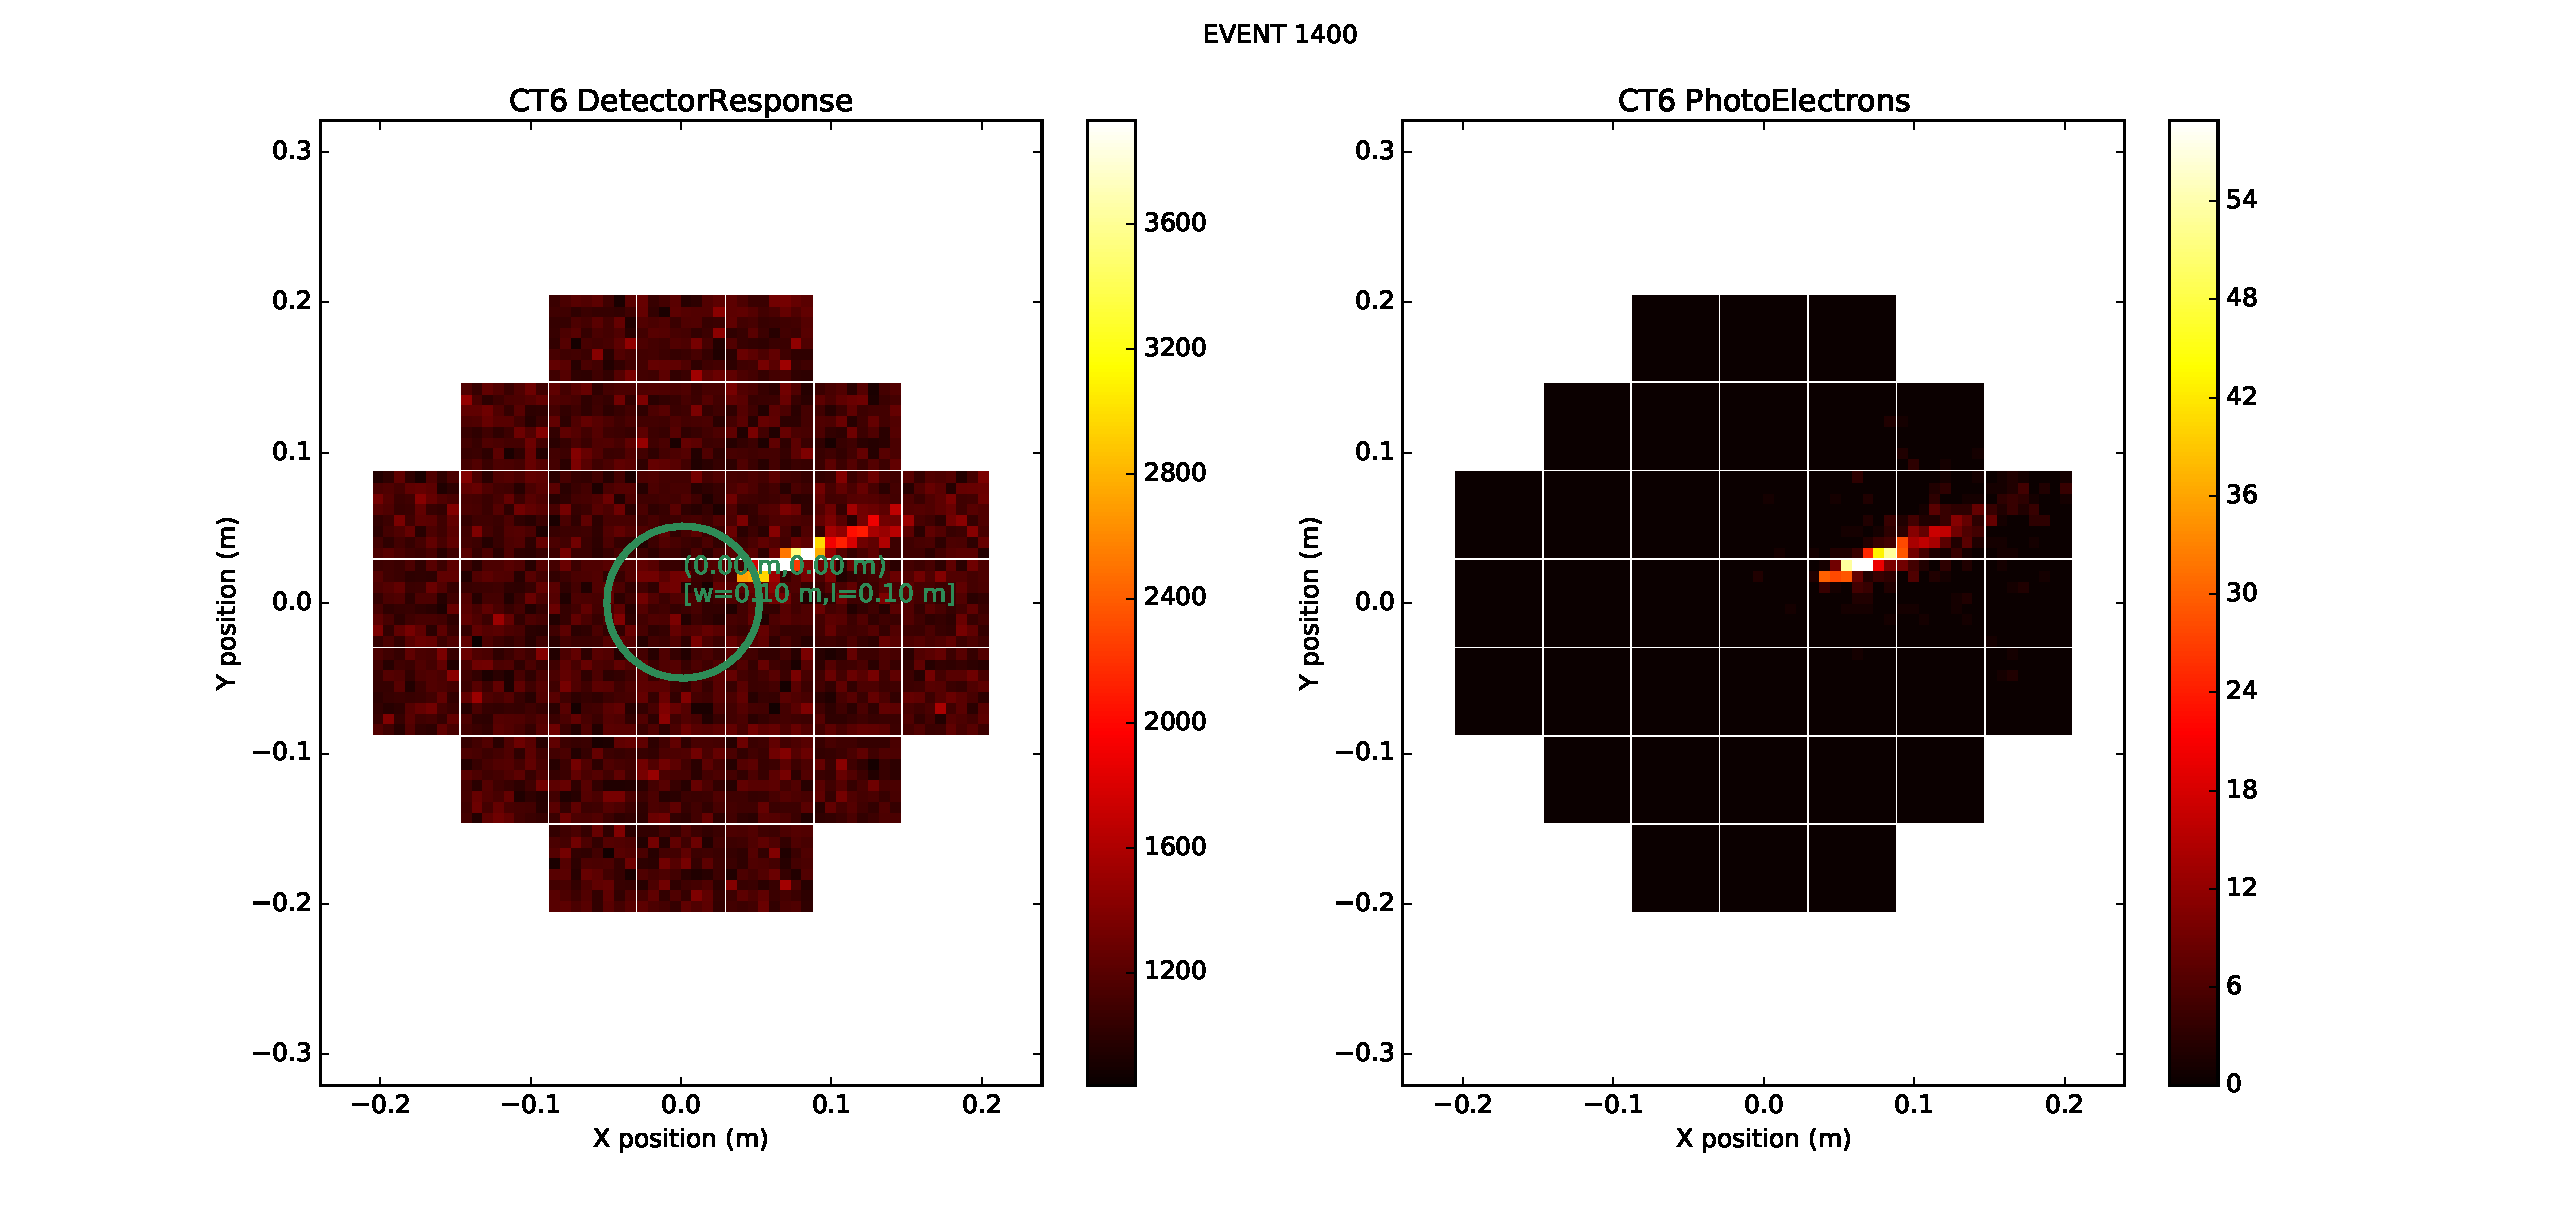
\includegraphics[trim=22cm 0 4cm 2cm,clip,width=.6\textwidth]{pics/photon_1}};
                    \node[anchor=north] (pic2) at (pic1.south){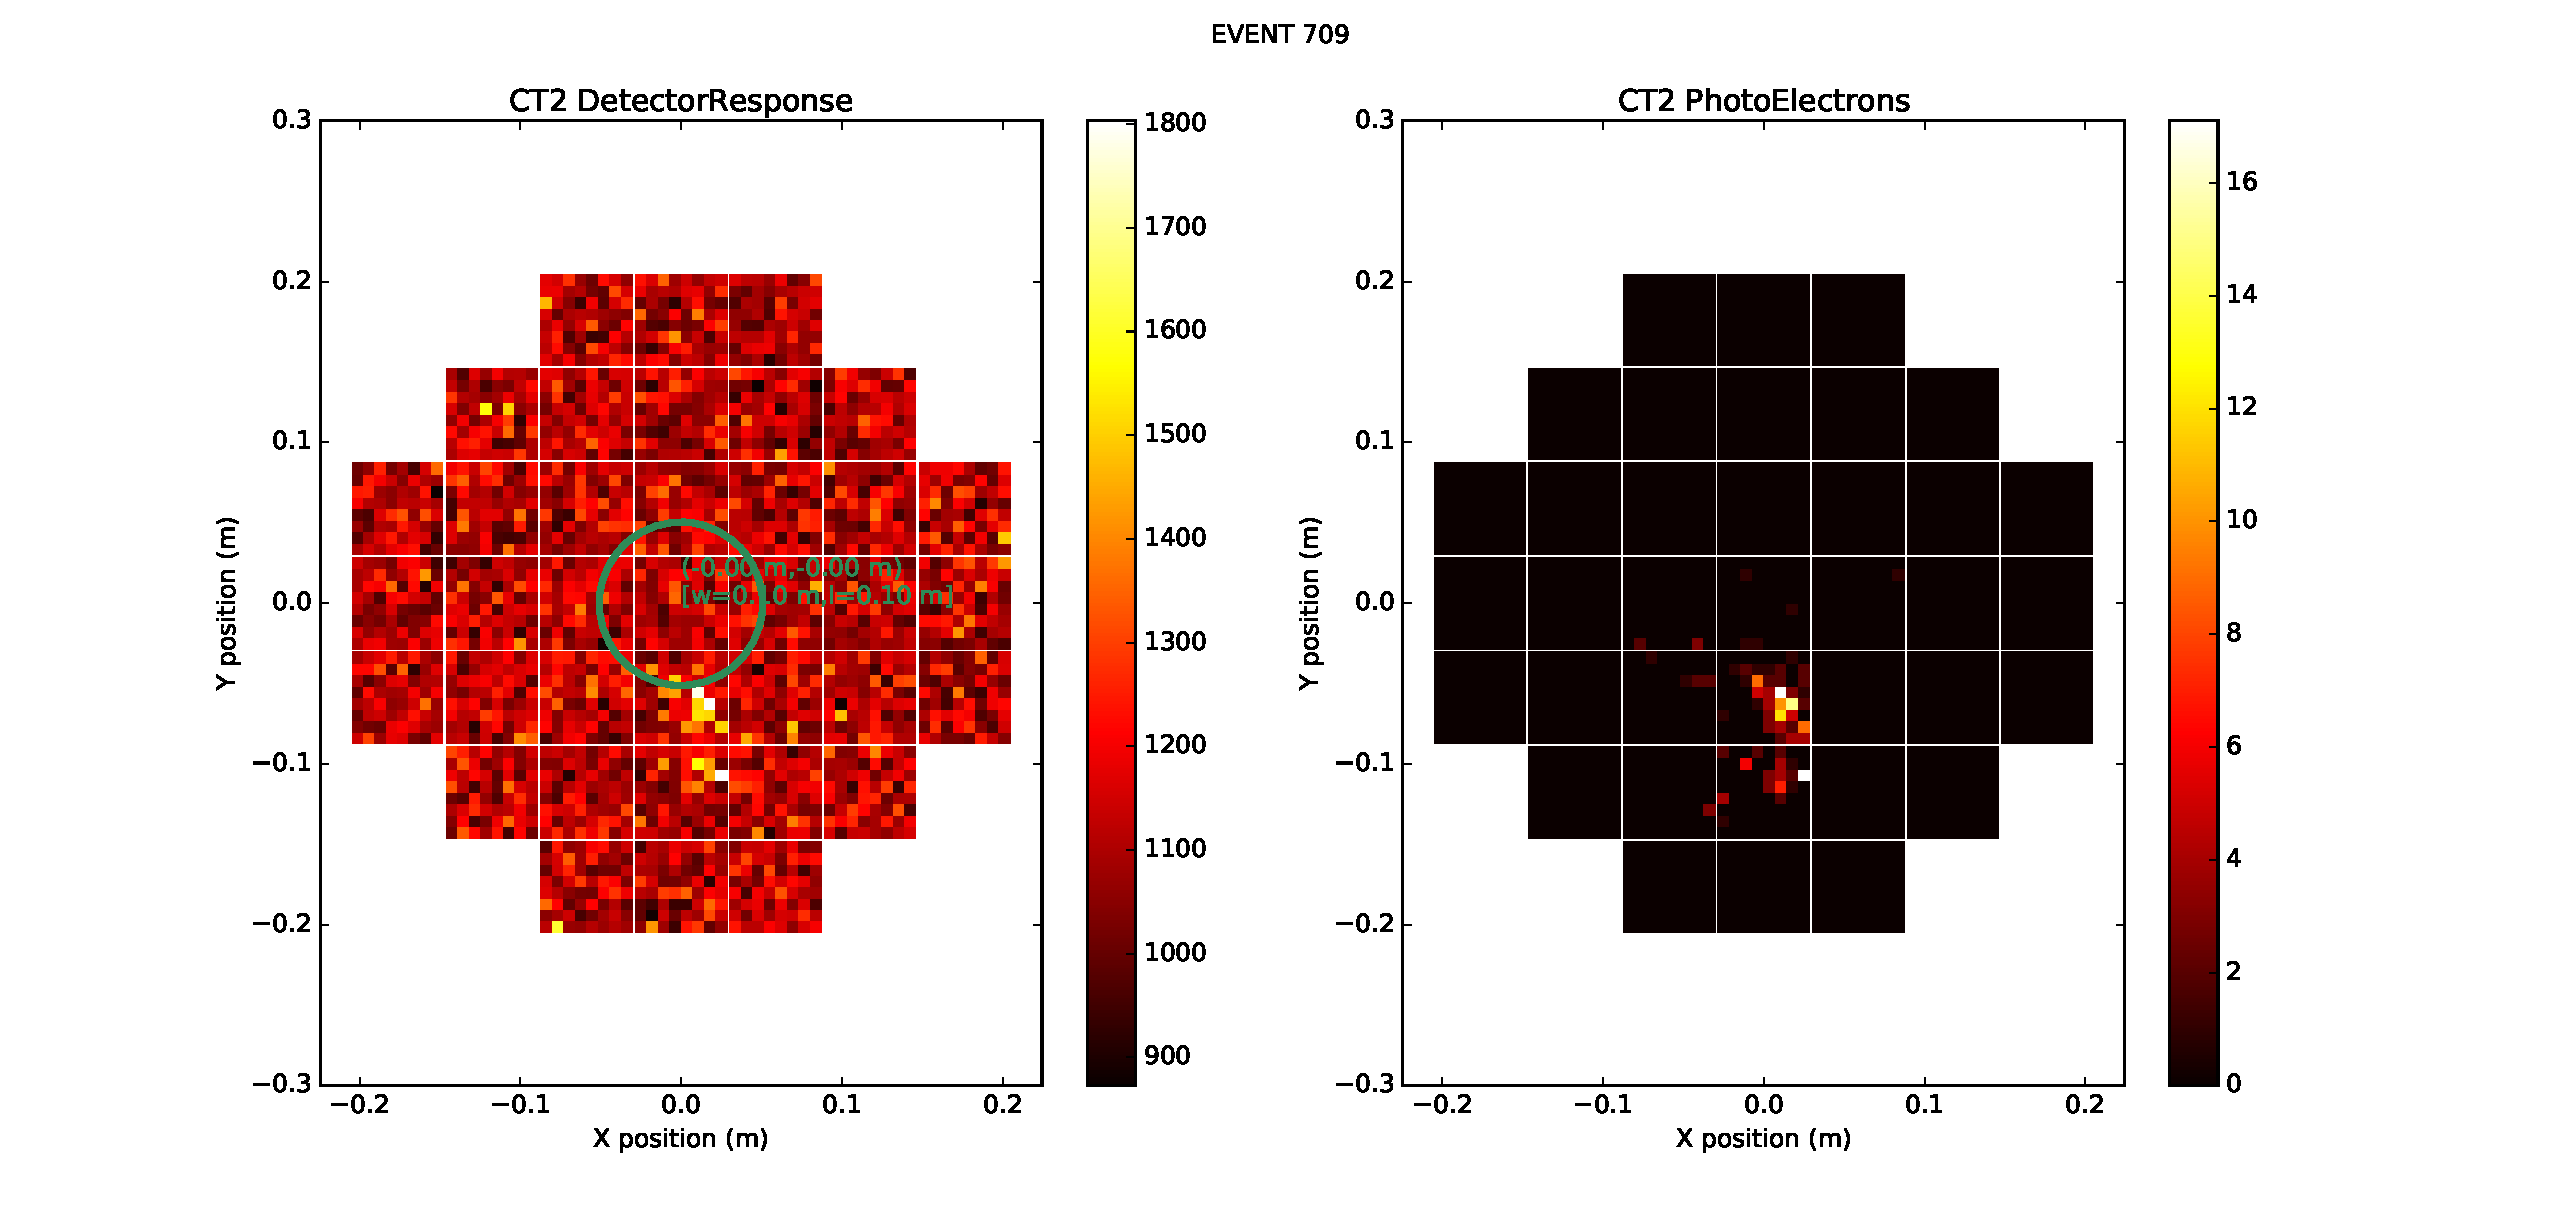
\includegraphics[trim=22cm 0 4cm 2cm,clip,width=.6\textwidth]{pics/proton_1}};
                    \node[anchor=south,rotate=90] at (pic1.west) {photon};
                    \node[anchor=south,rotate=90] at (pic2.west) {proton};
                \end{tikzpicture}
        \end{columns}
    \end{frame}
    
    
    \begin{frame}{Skymap of a point-source}
        \begin{columns}
            \column{.5\textwidth}
                \centering
                tail cuts\\
                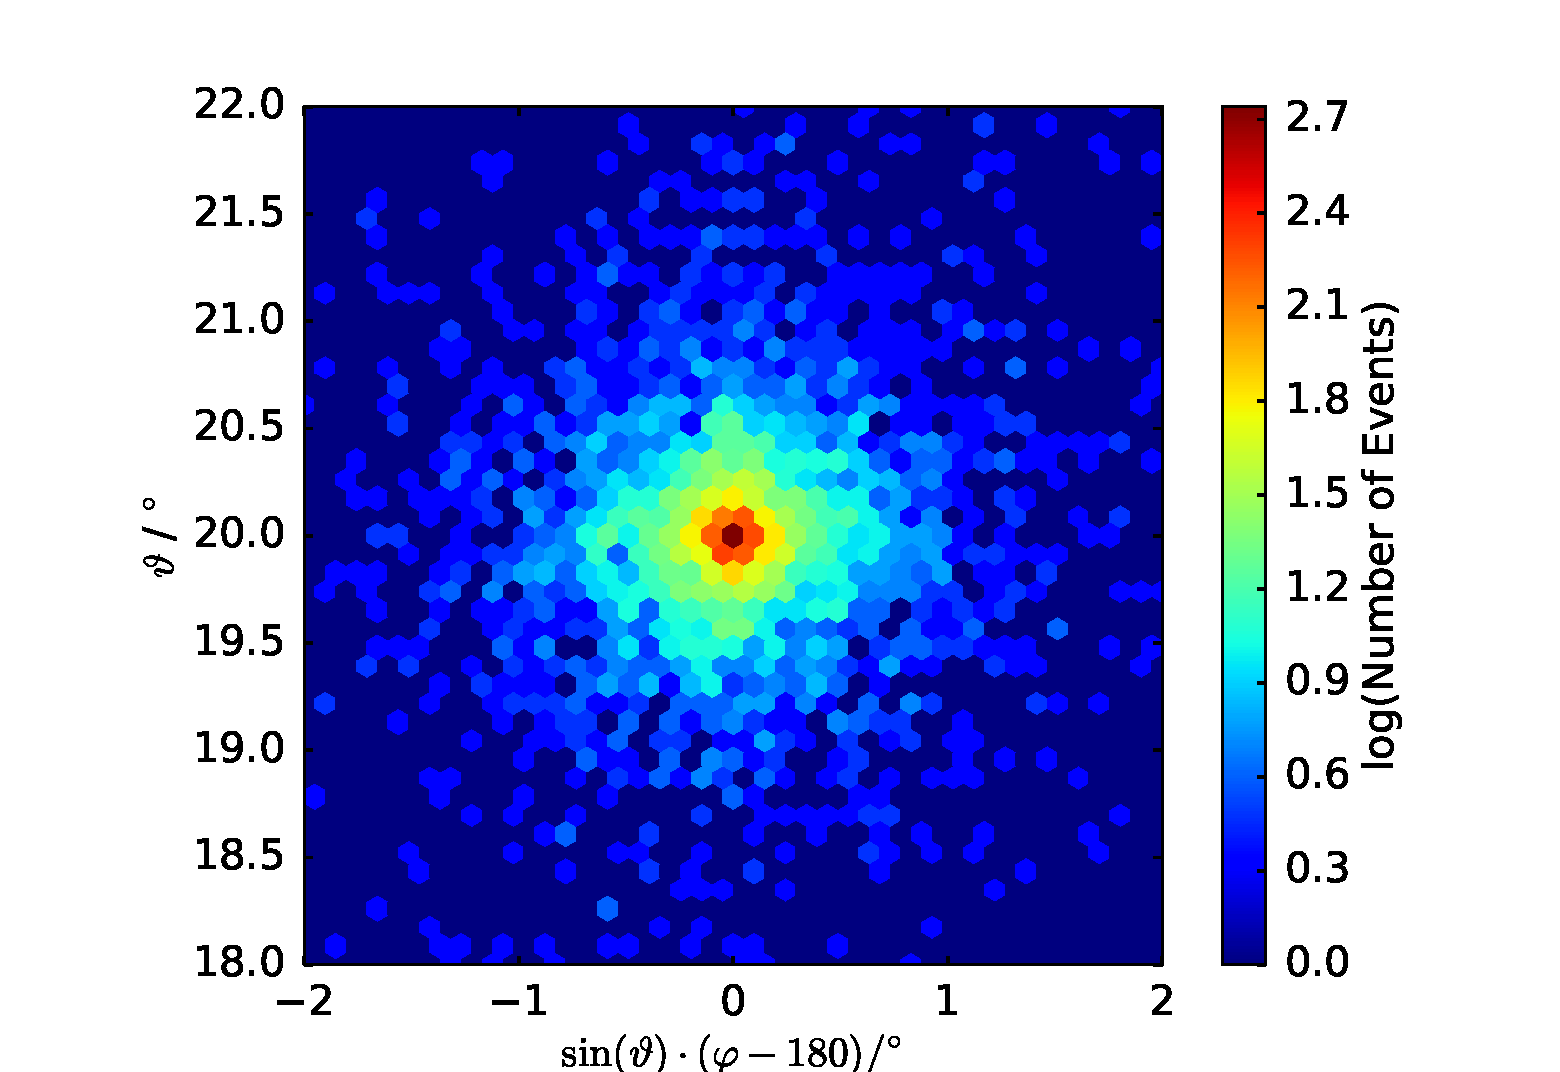
\includegraphics[trim=2.2cm 0 2.5cm 5mm,clip,width=.95\textwidth]{pics/CTA/skymap_tail.pdf}
            \column{.5\textwidth}
                \centering
                wavelets\\                
                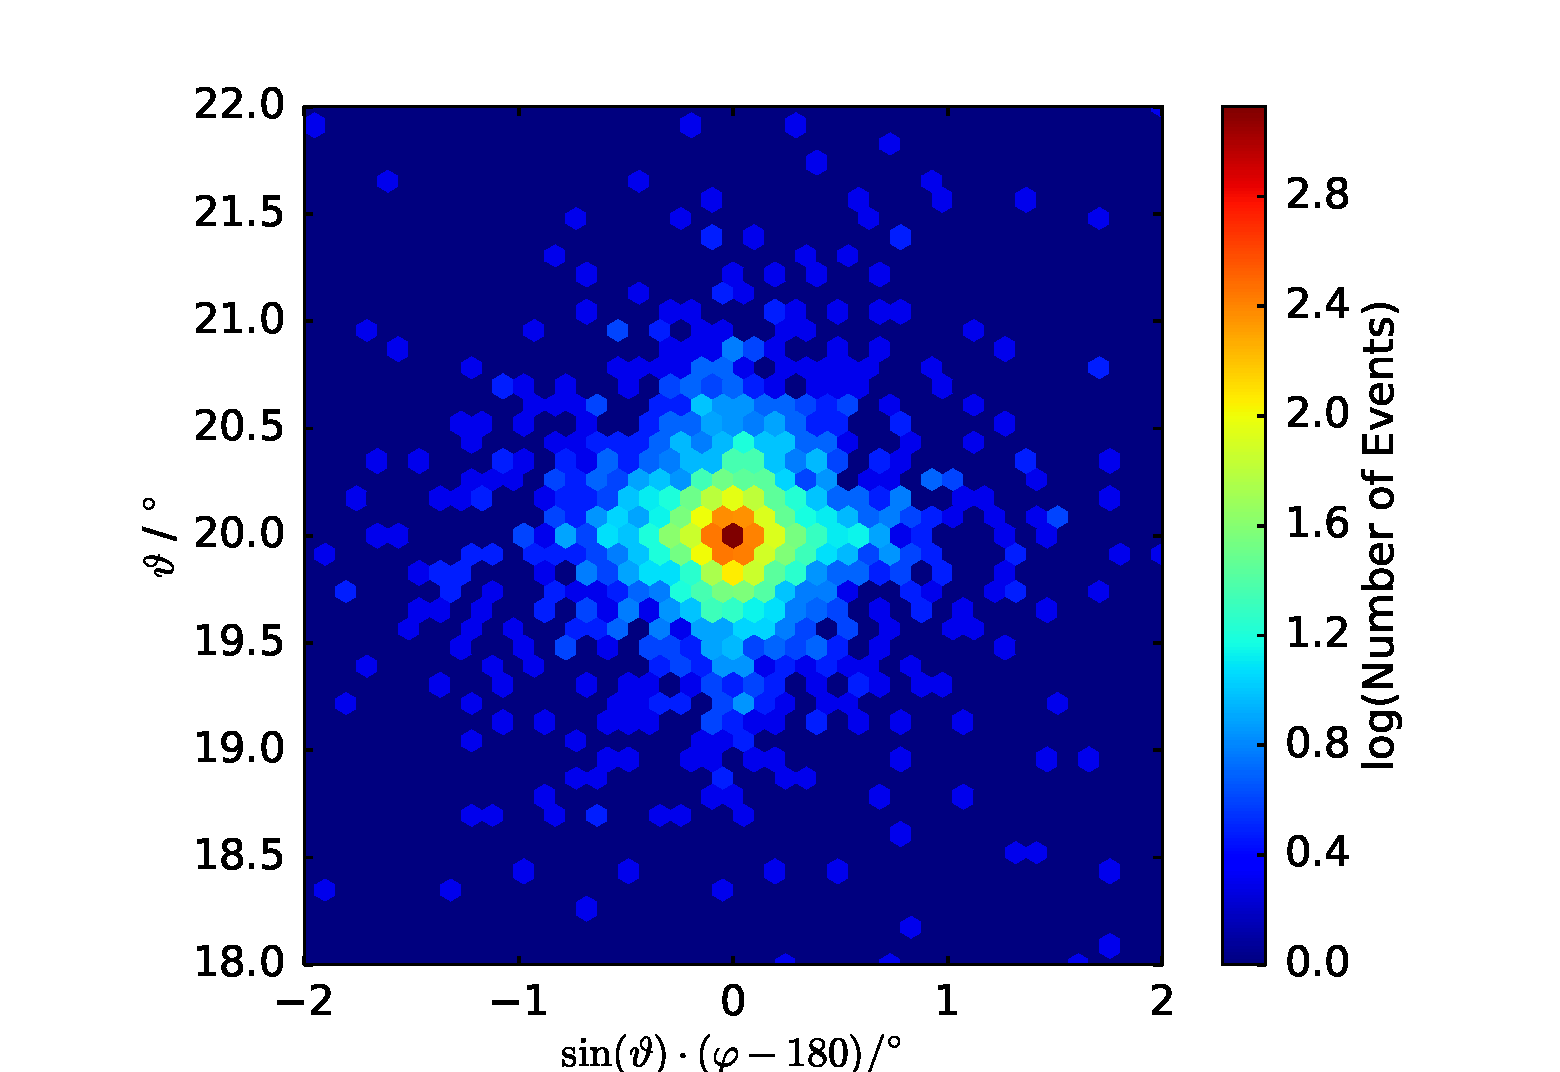
\includegraphics[trim=2.2cm 0 2.5cm 5mm,clip,width=.95\textwidth]{pics/CTA/skymap_wave.pdf}
        \end{columns}

    \end{frame}

    

    \begin{frame}{Conclusion}{}
        {\Large
        \centering
        \begin{itemize}
            \item apply analysis chain to full array
            \item investigate
            \begin{itemize}
            {\large
                \item impact on overlapping sources
                \item real-time analysis
                \item $\rightarrow$ reduction of data flow
            }
            \end{itemize}
            \item[]
            \item for more information on wavelets:\\
                see Jérémie's talk in February
            \item will be here for another 1,5 years
        \end{itemize}
        }
    \end{frame}

    
    \newcounter{finalframe}
    \setcounter{finalframe}{\value{framenumber}}

    
%     \end{document}
    
    
    
    \begin{frame}
        \centering
        \Huge Backup\\
    \end{frame}


    \begin{frame}
        \frametitle{Muon Track Reconstruction}
        \begin{columns}
            \column{.55\textwidth}
                \begin{itemize}
                    \item muon track reconstruction already well established
                    \item muons can pass through detector
                    \item Cherenkov radiation along track
                    \item photons emitted at $\varphi_\mathrm{Ch}\approx\unit{42}{\degree}$
                    \item clean signature 
                    \item[]
                    \item maximum likelihood fit based on hit time residuals
                    \item median angular resolution $\approx\unit{0.4}{\degree}$ 
                    \item[]
                    \item limit us to $\nu_\mu \rightarrow \mu$ (and $\nu_\tau \rightarrow \tau \rightarrow\mu$) interactions

                \end{itemize}
            \column{.45\textwidth}
                \begin{tikzpicture}
                    \coordinate (vert) at (1.5,1.);
                    \draw [line width=4mm,join=round,blue!0] (-0.5,-1.5)  rectangle (4,6);
                    \draw [line width=4mm,join=round,blue!10,fill=blue!10] (-0.5,0)  rectangle (4,5);
                    \draw[dashed,-stealth] (1,0) -- (vert) node[midway,right] {$\nu_\mu$};
                    \fill[black] (vert) circle (1.5pt);
                    \draw[-stealth] (vert) -- +(80:3.5) node [midway,left] {$\mu$} coordinate (muend);
                    \draw[blue,snake it,-stealth] ($(vert) ! .1 ! (muend)$) -- +( 38:1.6) ;
                    \draw[blue,snake it,-stealth] ($(vert) ! .4 ! (muend)$) -- +( 38:1.6) ;
                    \draw[blue,snake it,-stealth] ($(vert) ! .8 ! (muend)$) -- +( 38:1.6) node [label=0:{$\gamma$}] {};
                    \draw[blue,snake it,-stealth] ($(vert) ! .3 ! (muend)$) -- +(122:1.6) ;
                    \draw[blue,snake it,-stealth] ($(vert) ! .7 ! (muend)$) -- +(122:1.6) ;
                
                \end{tikzpicture}
        \end{columns}
    \end{frame}

    \begin{frame}
        \frametitle{Shower Reconstruction}
        \begin{columns}
            \column{.55\textwidth}
                \begin{itemize}
                    \item shower events open window to \\
                        {}\hspace{12pt}$\nu_e \rightarrow e$\\
                        {}\hspace{12pt}$\nu_x \rightarrow \nu_x + hadr.$ \\
                        {}\hspace{12pt}$\nu_\tau \rightarrow \tau \rightarrow e / hadr.$
                    \item[]
                    \item cascade of particles within few metres
                    \item can be approximated as point source
                    \item emits shell of light in all directions
                    \item still, more light emitted under ``Cherenkov angle''
                    \item[]
                    \item[] in ice: 
                    \item effect almost completely gone due to scattering
                \end{itemize}
            \column{.45\textwidth}

                \begin{tikzpicture}
                    \coordinate (vert) at (1.5,1.);
                    \draw [line width=4mm,join=round,blue!0] (-0.5,-1.5)  rectangle (4,6);
                \only<1>{
                    \draw [line width=4mm,join=round,blue!10,fill=blue!10] (-0.5,0)  rectangle (4,5);
                    \draw[dashed,-stealth] (1,0) -- (vert) node[midway,right] {$\nu_e$};
                    \fill[black] (vert) circle (1.5pt);
                    \draw (vert) -- +(70:.5);
                    \draw (vert) -- +(89:.5);
                    \draw ([shift=(78:.3)]vert) -- +(60:.5);
                    \draw ([shift=(82:.3)]vert) -- +(100:.5);
                    
                    \draw ([shift=(80:.5)]vert) -- +(74:.5);           \draw ([shift=(85:.5)]vert) -- +(90:.5);
                    \draw ([shift=(70:.6)]vert) -- +(70:.5);           \draw ([shift=(90:.6)]vert) -- +(91:.5);
                    \draw ([shift=(70:.6)]vert) -- +(50:.5);           \draw ([shift=(90:.6)]vert) -- +(110:.5);
                    \draw ([shift=(75:.9)]vert) -- +(75:.5);           \draw ([shift=(85:.9)]vert) -- +(85:.5);
                    \draw ([shift=(75:1.1)]vert) -- +(70:.5);          \draw ([shift=(85:1.1)]vert) -- +(90:.5);
                    \draw ([shift=(65:1.1)]vert) -- +(85:.5);          \draw ([shift=(95:1.1)]vert) -- +(75:.5);
                    \draw ([shift=(78:1.1)]vert) -- +(50:.5);          \draw ([shift=(82:1.1)]vert) -- +(110:.5);
                    \draw ([shift=(77:1.3)]vert) -- +(80:.5);          \draw ([shift=(83:1.3)]vert) -- +(80:.5);
                    \draw ([shift=(75:1.5)]vert) -- +(70:.5);          \draw ([shift=(85:1.5)]vert) -- +(91:.5);
                    \draw ([shift=(69:1.5)]vert) -- +(85:.5);          \draw ([shift=(91:1.5)]vert) -- +(75:.5);
                    \draw ([shift=(65:1.5)]vert) -- +(65:.5);          \draw ([shift=(95:1.5)]vert) -- +(95:.5);
                    \draw ([shift=(66:.9)]vert) -- +(65:.5);           \draw ([shift=(94:.9)]vert) -- +(95:.5);
                    \draw ([shift=(71:1.15)]vert) -- +(65:.5);         \draw ([shift=(89:1.15)]vert) -- +(95:.5);
                    \draw ([shift=(71:2.1)]vert) -- +(67:.5);          \draw ([shift=(89:2.1)]vert) -- +(93:.5);
                    \draw ([shift=(68:1.7)]vert) -- +(70:.5);          \draw ([shift=(92:1.7)]vert) -- +(91:.5);
                    \draw ([shift=(78:1.85)]vert) -- +(75:.5);         \draw ([shift=(82:1.85)]vert) -- +(85:.5);
                    \draw ([shift=(74:2.05)]vert) -- +(70:.5);         \draw ([shift=(86:2.05)]vert) -- +(91:.5);
                    \draw ([shift=(79:2.5)]vert) -- +(65:.5);          \draw ([shift=(81:2.5)]vert) -- +(95:.5);
                    \draw ([shift=(80:2.2)]vert) -- +(80:.5);          \draw ([shift=(80:.9)]vert) -- +(80:.7);
                    \draw ([shift=(82:2.5)]vert) -- +(79:.5);          \draw ([shift=(79:2.6)]vert) -- +(82:.5);
                    \draw ([shift=(76:2.4)]vert) -- +(55:.5);          \draw ([shift=(84:2.4)]vert) -- +(105:.5);
                    \draw ([shift=(69:1.5)]vert) -- +(60:.5);          \draw ([shift=(91:1.5)]vert) -- +(100:.5);
                    \draw ([shift=(67:1.1)]vert) -- +(50:.5);          \draw ([shift=(93:1.1)]vert) -- +(110:.5);
                    \draw[blue,snake it,-stealth] ([shift=(100:2.5)]vert) -- +(122:1.6) ;
                    \draw[blue,snake it,-stealth] ([shift=(55:2.2)]vert) -- +(38:1.6) node [label=180:{$\gamma$}] {};
                    \draw[blue,snake it,-stealth] ([shift=(45:1.5)]vert) -- +(-20:1.6) ;
                    \draw[blue,snake it,-stealth] ([shift=(120:1.)]vert) -- +(200:1.6) ;
                }
                \only<2>{
                    \node[anchor=north ] (cosphi) at (1.7,4.5) {
                        \resizebox{\textwidth}{!}{
                            \pgfdeclareplotmark{cross} {
\pgfpathmoveto{\pgfpoint{-0.3\pgfplotmarksize}{\pgfplotmarksize}}
\pgfpathlineto{\pgfpoint{+0.3\pgfplotmarksize}{\pgfplotmarksize}}
\pgfpathlineto{\pgfpoint{+0.3\pgfplotmarksize}{0.3\pgfplotmarksize}}
\pgfpathlineto{\pgfpoint{+1\pgfplotmarksize}{0.3\pgfplotmarksize}}
\pgfpathlineto{\pgfpoint{+1\pgfplotmarksize}{-0.3\pgfplotmarksize}}
\pgfpathlineto{\pgfpoint{+0.3\pgfplotmarksize}{-0.3\pgfplotmarksize}}
\pgfpathlineto{\pgfpoint{+0.3\pgfplotmarksize}{-1.\pgfplotmarksize}}
\pgfpathlineto{\pgfpoint{-0.3\pgfplotmarksize}{-1.\pgfplotmarksize}}
\pgfpathlineto{\pgfpoint{-0.3\pgfplotmarksize}{-0.3\pgfplotmarksize}}
\pgfpathlineto{\pgfpoint{-1.\pgfplotmarksize}{-0.3\pgfplotmarksize}}
\pgfpathlineto{\pgfpoint{-1.\pgfplotmarksize}{0.3\pgfplotmarksize}}
\pgfpathlineto{\pgfpoint{-0.3\pgfplotmarksize}{0.3\pgfplotmarksize}}
\pgfpathclose
\pgfusepathqstroke
}
\pgfdeclareplotmark{cross*} {
\pgfpathmoveto{\pgfpoint{-0.3\pgfplotmarksize}{\pgfplotmarksize}}
\pgfpathlineto{\pgfpoint{+0.3\pgfplotmarksize}{\pgfplotmarksize}}
\pgfpathlineto{\pgfpoint{+0.3\pgfplotmarksize}{0.3\pgfplotmarksize}}
\pgfpathlineto{\pgfpoint{+1\pgfplotmarksize}{0.3\pgfplotmarksize}}
\pgfpathlineto{\pgfpoint{+1\pgfplotmarksize}{-0.3\pgfplotmarksize}}
\pgfpathlineto{\pgfpoint{+0.3\pgfplotmarksize}{-0.3\pgfplotmarksize}}
\pgfpathlineto{\pgfpoint{+0.3\pgfplotmarksize}{-1.\pgfplotmarksize}}
\pgfpathlineto{\pgfpoint{-0.3\pgfplotmarksize}{-1.\pgfplotmarksize}}
\pgfpathlineto{\pgfpoint{-0.3\pgfplotmarksize}{-0.3\pgfplotmarksize}}
\pgfpathlineto{\pgfpoint{-1.\pgfplotmarksize}{-0.3\pgfplotmarksize}}
\pgfpathlineto{\pgfpoint{-1.\pgfplotmarksize}{0.3\pgfplotmarksize}}
\pgfpathlineto{\pgfpoint{-0.3\pgfplotmarksize}{0.3\pgfplotmarksize}}
\pgfpathclose
\pgfusepathqfillstroke
}
\pgfdeclareplotmark{newstar} {
\pgfpathmoveto{\pgfqpoint{0pt}{\pgfplotmarksize}}
\pgfpathlineto{\pgfqpointpolar{44}{0.5\pgfplotmarksize}}
\pgfpathlineto{\pgfqpointpolar{18}{\pgfplotmarksize}}
\pgfpathlineto{\pgfqpointpolar{-20}{0.5\pgfplotmarksize}}
\pgfpathlineto{\pgfqpointpolar{-54}{\pgfplotmarksize}}
\pgfpathlineto{\pgfqpointpolar{-90}{0.5\pgfplotmarksize}}
\pgfpathlineto{\pgfqpointpolar{234}{\pgfplotmarksize}}
\pgfpathlineto{\pgfqpointpolar{198}{0.5\pgfplotmarksize}}
\pgfpathlineto{\pgfqpointpolar{162}{\pgfplotmarksize}}
\pgfpathlineto{\pgfqpointpolar{134}{0.5\pgfplotmarksize}}
\pgfpathclose
\pgfusepathqstroke
}
\pgfdeclareplotmark{newstar*} {
\pgfpathmoveto{\pgfqpoint{0pt}{\pgfplotmarksize}}
\pgfpathlineto{\pgfqpointpolar{44}{0.5\pgfplotmarksize}}
\pgfpathlineto{\pgfqpointpolar{18}{\pgfplotmarksize}}
\pgfpathlineto{\pgfqpointpolar{-20}{0.5\pgfplotmarksize}}
\pgfpathlineto{\pgfqpointpolar{-54}{\pgfplotmarksize}}
\pgfpathlineto{\pgfqpointpolar{-90}{0.5\pgfplotmarksize}}
\pgfpathlineto{\pgfqpointpolar{234}{\pgfplotmarksize}}
\pgfpathlineto{\pgfqpointpolar{198}{0.5\pgfplotmarksize}}
\pgfpathlineto{\pgfqpointpolar{162}{\pgfplotmarksize}}
\pgfpathlineto{\pgfqpointpolar{134}{0.5\pgfplotmarksize}}
\pgfpathclose
\pgfusepathqfillstroke
}
\begin{tikzpicture}
\definecolor{c}{rgb}{1,1,1};
\draw [color=c, fill=c] (0,0) rectangle (20,14.6154);
\draw [color=c, fill=c] (3.2,2.33846) rectangle (18.4,13.7385);
\definecolor{c}{rgb}{0,0,0};
\draw [c] (3.2,2.33846) -- (3.2,13.7385) -- (18.4,13.7385) -- (18.4,2.33846) -- (3.2,2.33846);
\definecolor{c}{rgb}{1,1,1};
\draw [color=c, fill=c] (3.2,2.33846) rectangle (18.4,13.7385);
\definecolor{c}{rgb}{0,0,0};
\draw [c] (3.2,2.33846) -- (3.2,13.7385) -- (18.4,13.7385) -- (18.4,2.33846) -- (3.2,2.33846);
\definecolor{c}{rgb}{0,0,0.6};
\draw [c,line width=1] (3.2,2.5239) -- (3.352,2.5239) -- (3.352,2.51622) -- (3.504,2.51622) -- (3.504,2.51806) -- (3.656,2.51806) -- (3.656,2.53372) -- (3.808,2.53372) -- (3.808,2.53502) -- (3.96,2.53502) -- (3.96,2.53867) -- (4.112,2.53867) --
 (4.112,2.53073) -- (4.264,2.53073) -- (4.264,2.5437) -- (4.416,2.5437) -- (4.416,2.54808) -- (4.568,2.54808) -- (4.568,2.54401) -- (4.72,2.54401) -- (4.72,2.55009) -- (4.872,2.55009) -- (4.872,2.57481) -- (5.024,2.57481) -- (5.024,2.5814) --
 (5.176,2.5814) -- (5.176,2.57783) -- (5.328,2.57783) -- (5.328,2.57043) -- (5.48,2.57043) -- (5.48,2.57323) -- (5.632,2.57323) -- (5.632,2.57014) -- (5.784,2.57014) -- (5.784,2.60634) -- (5.936,2.60634) -- (5.936,2.5855) -- (6.088,2.5855) --
 (6.088,2.61015) -- (6.24,2.61015) -- (6.24,2.58806) -- (6.392,2.58806) -- (6.392,2.60112) -- (6.544,2.60112) -- (6.544,2.61234) -- (6.696,2.61234) -- (6.696,2.6286) -- (6.848,2.6286) -- (6.848,2.63319) -- (7,2.63319) -- (7,2.61981) --
 (7.152,2.61981) -- (7.152,2.62429) -- (7.304,2.62429) -- (7.304,2.66068) -- (7.456,2.66068) -- (7.456,2.65785) -- (7.608,2.65785) -- (7.608,2.64971) -- (7.76,2.64971) -- (7.76,2.65388) -- (7.912,2.65388) -- (7.912,2.67308) -- (8.064,2.67308) --
 (8.064,2.69335) -- (8.216,2.69335) -- (8.216,2.6948) -- (8.368,2.6948) -- (8.368,2.68229) -- (8.52,2.68229) -- (8.52,2.72453) -- (8.672,2.72453) -- (8.672,2.7174) -- (8.824,2.7174) -- (8.824,2.7237) -- (8.976,2.7237) -- (8.976,2.74433) --
 (9.128,2.74433) -- (9.128,2.76805) -- (9.28,2.76805) -- (9.28,2.77451) -- (9.432,2.77451) -- (9.432,2.82305) -- (9.584,2.82305) -- (9.584,2.79597) -- (9.736,2.79597) -- (9.736,2.78685) -- (9.888,2.78685) -- (9.888,2.81968) -- (10.04,2.81968) --
 (10.04,2.85795) -- (10.192,2.85795) -- (10.192,2.85118) -- (10.344,2.85118) -- (10.344,2.89718) -- (10.496,2.89718) -- (10.496,2.91868) -- (10.648,2.91868) -- (10.648,2.90298) -- (10.8,2.90298) -- (10.8,2.97664) -- (10.952,2.97664) --
 (10.952,2.96969) -- (11.104,2.96969) -- (11.104,3.0063) -- (11.256,3.0063) -- (11.256,2.99144) -- (11.408,2.99144) -- (11.408,3.02408) -- (11.56,3.02408) -- (11.56,3.07917) -- (11.712,3.07917) -- (11.712,3.14752) -- (11.864,3.14752) --
 (11.864,3.08028) -- (12.016,3.08028) -- (12.016,3.17096) -- (12.168,3.17096) -- (12.168,3.17061) -- (12.32,3.17061) -- (12.32,3.26598) -- (12.472,3.26598) -- (12.472,3.29968) -- (12.624,3.29968) -- (12.624,3.34746) -- (12.776,3.34746) --
 (12.776,3.33425) -- (12.928,3.33425) -- (12.928,3.43111) -- (13.08,3.43111) -- (13.08,3.46576) -- (13.232,3.46576) -- (13.232,3.57994) -- (13.384,3.57994) -- (13.384,3.55805) -- (13.536,3.55805) -- (13.536,3.66503) -- (13.688,3.66503) --
 (13.688,3.81528) -- (13.84,3.81528) -- (13.84,3.80736) -- (13.992,3.80736) -- (13.992,3.93111) -- (14.144,3.93111) -- (14.144,4.01146) -- (14.296,4.01146) -- (14.296,4.16707) -- (14.448,4.16707) -- (14.448,4.30494) -- (14.6,4.30494) --
 (14.6,4.51753) -- (14.752,4.51753) -- (14.752,4.69848) -- (14.904,4.69848) -- (14.904,4.92869) -- (15.056,4.92869) -- (15.056,5.17124) -- (15.208,5.17124) -- (15.208,5.38623) -- (15.36,5.38623) -- (15.36,5.73496) -- (15.512,5.73496) --
 (15.512,6.07259) -- (15.664,6.07259) -- (15.664,6.55439) -- (15.816,6.55439) -- (15.816,7.22868) -- (15.968,7.22868) -- (15.968,8.1099) -- (16.12,8.1099) -- (16.12,9.39988) -- (16.272,9.39988) -- (16.272,11.3371) -- (16.424,11.3371) --
 (16.424,13.1956) -- (16.576,13.1956) -- (16.576,11.6906) -- (16.728,11.6906) -- (16.728,9.90987) -- (16.88,9.90987) -- (16.88,8.60399) -- (17.032,8.60399) -- (17.032,7.9837) -- (17.184,7.9837) -- (17.184,7.21555) -- (17.336,7.21555) --
 (17.336,6.62375) -- (17.488,6.62375) -- (17.488,6.13286) -- (17.64,6.13286) -- (17.64,5.82593) -- (17.792,5.82593) -- (17.792,5.53839) -- (17.944,5.53839) -- (17.944,5.36948) -- (18.096,5.36948) -- (18.096,5.0261) -- (18.248,5.0261) --
 (18.248,4.99034) -- (18.4,4.99034);
\definecolor{c}{rgb}{0,0,0};
\draw [c,line width=1] (3.2,2.33846) -- (18.4,2.33846);
\draw [anchor= east] (18.4,0.584615) node[scale=3, rotate=0]{$\cos(\varphi)$};
\draw [c,line width=1] (3.2,2.67169) -- (3.2,2.33846);
\draw [c,line width=1] (3.58,2.50508) -- (3.58,2.33846);
\draw [c,line width=1] (3.96,2.50508) -- (3.96,2.33846);
\draw [c,line width=1] (4.34,2.50508) -- (4.34,2.33846);
\draw [c,line width=1] (4.72,2.67169) -- (4.72,2.33846);
\draw [c,line width=1] (5.1,2.50508) -- (5.1,2.33846);
\draw [c,line width=1] (5.48,2.50508) -- (5.48,2.33846);
\draw [c,line width=1] (5.86,2.50508) -- (5.86,2.33846);
\draw [c,line width=1] (6.24,2.67169) -- (6.24,2.33846);
\draw [c,line width=1] (6.62,2.50508) -- (6.62,2.33846);
\draw [c,line width=1] (7,2.50508) -- (7,2.33846);
\draw [c,line width=1] (7.38,2.50508) -- (7.38,2.33846);
\draw [c,line width=1] (7.76,2.67169) -- (7.76,2.33846);
\draw [c,line width=1] (8.14,2.50508) -- (8.14,2.33846);
\draw [c,line width=1] (8.52,2.50508) -- (8.52,2.33846);
\draw [c,line width=1] (8.9,2.50508) -- (8.9,2.33846);
\draw [c,line width=1] (9.28,2.67169) -- (9.28,2.33846);
\draw [c,line width=1] (9.66,2.50508) -- (9.66,2.33846);
\draw [c,line width=1] (10.04,2.50508) -- (10.04,2.33846);
\draw [c,line width=1] (10.42,2.50508) -- (10.42,2.33846);
\draw [c,line width=1] (10.8,2.67169) -- (10.8,2.33846);
\draw [c,line width=1] (11.18,2.50508) -- (11.18,2.33846);
\draw [c,line width=1] (11.56,2.50508) -- (11.56,2.33846);
\draw [c,line width=1] (11.94,2.50508) -- (11.94,2.33846);
\draw [c,line width=1] (12.32,2.67169) -- (12.32,2.33846);
\draw [c,line width=1] (12.7,2.50508) -- (12.7,2.33846);
\draw [c,line width=1] (13.08,2.50508) -- (13.08,2.33846);
\draw [c,line width=1] (13.46,2.50508) -- (13.46,2.33846);
\draw [c,line width=1] (13.84,2.67169) -- (13.84,2.33846);
\draw [c,line width=1] (14.22,2.50508) -- (14.22,2.33846);
\draw [c,line width=1] (14.6,2.50508) -- (14.6,2.33846);
\draw [c,line width=1] (14.98,2.50508) -- (14.98,2.33846);
\draw [c,line width=1] (15.36,2.67169) -- (15.36,2.33846);
\draw [c,line width=1] (15.74,2.50508) -- (15.74,2.33846);
\draw [c,line width=1] (16.12,2.50508) -- (16.12,2.33846);
\draw [c,line width=1] (16.5,2.50508) -- (16.5,2.33846);
\draw [c,line width=1] (16.88,2.67169) -- (16.88,2.33846);
\draw [c,line width=1] (17.26,2.50508) -- (17.26,2.33846);
\draw [c,line width=1] (17.64,2.50508) -- (17.64,2.33846);
\draw [c,line width=1] (18.02,2.50508) -- (18.02,2.33846);
\draw [c,line width=1] (18.4,2.67169) -- (18.4,2.33846);
\draw [c,line width=1] (3.2,2.67169) -- (3.2,2.33846);
\draw [anchor=base] (3.2,1.53462) node[scale=3, rotate=0]{-1};
\draw [anchor=base] (4.72,1.53462) node[scale=3, rotate=0]{-0.8};
\draw [anchor=base] (6.24,1.53462) node[scale=3, rotate=0]{-0.6};
\draw [anchor=base] (7.76,1.53462) node[scale=3, rotate=0]{-0.4};
\draw [anchor=base] (9.28,1.53462) node[scale=3, rotate=0]{-0.2};
\draw [anchor=base] (10.8,1.53462) node[scale=3, rotate=0]{0};
\draw [anchor=base] (12.32,1.53462) node[scale=3, rotate=0]{0.2};
\draw [anchor=base] (13.84,1.53462) node[scale=3, rotate=0]{0.4};
\draw [anchor=base] (15.36,1.53462) node[scale=3, rotate=0]{0.6};
\draw [anchor=base] (16.88,1.53462) node[scale=3, rotate=0]{0.8};
\draw [anchor=base] (18.4,1.53462) node[scale=3, rotate=0]{1};
\draw [c,line width=1] (3.2,13.7385) -- (18.4,13.7385);
\draw [c,line width=1] (3.2,13.4052) -- (3.2,13.7385);
\draw [c,line width=1] (3.58,13.5718) -- (3.58,13.7385);
\draw [c,line width=1] (3.96,13.5718) -- (3.96,13.7385);
\draw [c,line width=1] (4.34,13.5718) -- (4.34,13.7385);
\draw [c,line width=1] (4.72,13.4052) -- (4.72,13.7385);
\draw [c,line width=1] (5.1,13.5718) -- (5.1,13.7385);
\draw [c,line width=1] (5.48,13.5718) -- (5.48,13.7385);
\draw [c,line width=1] (5.86,13.5718) -- (5.86,13.7385);
\draw [c,line width=1] (6.24,13.4052) -- (6.24,13.7385);
\draw [c,line width=1] (6.62,13.5718) -- (6.62,13.7385);
\draw [c,line width=1] (7,13.5718) -- (7,13.7385);
\draw [c,line width=1] (7.38,13.5718) -- (7.38,13.7385);
\draw [c,line width=1] (7.76,13.4052) -- (7.76,13.7385);
\draw [c,line width=1] (8.14,13.5718) -- (8.14,13.7385);
\draw [c,line width=1] (8.52,13.5718) -- (8.52,13.7385);
\draw [c,line width=1] (8.9,13.5718) -- (8.9,13.7385);
\draw [c,line width=1] (9.28,13.4052) -- (9.28,13.7385);
\draw [c,line width=1] (9.66,13.5718) -- (9.66,13.7385);
\draw [c,line width=1] (10.04,13.5718) -- (10.04,13.7385);
\draw [c,line width=1] (10.42,13.5718) -- (10.42,13.7385);
\draw [c,line width=1] (10.8,13.4052) -- (10.8,13.7385);
\draw [c,line width=1] (11.18,13.5718) -- (11.18,13.7385);
\draw [c,line width=1] (11.56,13.5718) -- (11.56,13.7385);
\draw [c,line width=1] (11.94,13.5718) -- (11.94,13.7385);
\draw [c,line width=1] (12.32,13.4052) -- (12.32,13.7385);
\draw [c,line width=1] (12.7,13.5718) -- (12.7,13.7385);
\draw [c,line width=1] (13.08,13.5718) -- (13.08,13.7385);
\draw [c,line width=1] (13.46,13.5718) -- (13.46,13.7385);
\draw [c,line width=1] (13.84,13.4052) -- (13.84,13.7385);
\draw [c,line width=1] (14.22,13.5718) -- (14.22,13.7385);
\draw [c,line width=1] (14.6,13.5718) -- (14.6,13.7385);
\draw [c,line width=1] (14.98,13.5718) -- (14.98,13.7385);
\draw [c,line width=1] (15.36,13.4052) -- (15.36,13.7385);
\draw [c,line width=1] (15.74,13.5718) -- (15.74,13.7385);
\draw [c,line width=1] (16.12,13.5718) -- (16.12,13.7385);
\draw [c,line width=1] (16.5,13.5718) -- (16.5,13.7385);
\draw [c,line width=1] (16.88,13.4052) -- (16.88,13.7385);
\draw [c,line width=1] (17.26,13.5718) -- (17.26,13.7385);
\draw [c,line width=1] (17.64,13.5718) -- (17.64,13.7385);
\draw [c,line width=1] (18.02,13.5718) -- (18.02,13.7385);
\draw [c,line width=1] (18.4,13.4052) -- (18.4,13.7385);
\draw [c,line width=1] (3.2,13.4052) -- (3.2,13.7385);
\draw [c,line width=1] (3.2,2.33846) -- (3.2,13.7385);
\draw [anchor= east] (0.8,13.7385) node[scale=3, rotate=90]{expected Photons};
\draw [c,line width=1] (3.668,2.33846) -- (3.2,2.33846);
\draw [c,line width=1] (3.434,2.60957) -- (3.2,2.60957);
\draw [c,line width=1] (3.434,2.88068) -- (3.2,2.88068);
\draw [c,line width=1] (3.434,3.15179) -- (3.2,3.15179);
\draw [c,line width=1] (3.668,3.4229) -- (3.2,3.4229);
\draw [c,line width=1] (3.434,3.69401) -- (3.2,3.69401);
\draw [c,line width=1] (3.434,3.96513) -- (3.2,3.96513);
\draw [c,line width=1] (3.434,4.23624) -- (3.2,4.23624);
\draw [c,line width=1] (3.668,4.50735) -- (3.2,4.50735);
\draw [c,line width=1] (3.434,4.77846) -- (3.2,4.77846);
\draw [c,line width=1] (3.434,5.04957) -- (3.2,5.04957);
\draw [c,line width=1] (3.434,5.32068) -- (3.2,5.32068);
\draw [c,line width=1] (3.668,5.59179) -- (3.2,5.59179);
\draw [c,line width=1] (3.434,5.8629) -- (3.2,5.8629);
\draw [c,line width=1] (3.434,6.13401) -- (3.2,6.13401);
\draw [c,line width=1] (3.434,6.40512) -- (3.2,6.40512);
\draw [c,line width=1] (3.668,6.67623) -- (3.2,6.67623);
\draw [c,line width=1] (3.434,6.94734) -- (3.2,6.94734);
\draw [c,line width=1] (3.434,7.21845) -- (3.2,7.21845);
\draw [c,line width=1] (3.434,7.48956) -- (3.2,7.48956);
\draw [c,line width=1] (3.668,7.76067) -- (3.2,7.76067);
\draw [c,line width=1] (3.434,8.03179) -- (3.2,8.03179);
\draw [c,line width=1] (3.434,8.3029) -- (3.2,8.3029);
\draw [c,line width=1] (3.434,8.57401) -- (3.2,8.57401);
\draw [c,line width=1] (3.668,8.84512) -- (3.2,8.84512);
\draw [c,line width=1] (3.434,9.11623) -- (3.2,9.11623);
\draw [c,line width=1] (3.434,9.38734) -- (3.2,9.38734);
\draw [c,line width=1] (3.434,9.65845) -- (3.2,9.65845);
\draw [c,line width=1] (3.668,9.92956) -- (3.2,9.92956);
\draw [c,line width=1] (3.434,10.2007) -- (3.2,10.2007);
\draw [c,line width=1] (3.434,10.4718) -- (3.2,10.4718);
\draw [c,line width=1] (3.434,10.7429) -- (3.2,10.7429);
\draw [c,line width=1] (3.668,11.014) -- (3.2,11.014);
\draw [c,line width=1] (3.434,11.2851) -- (3.2,11.2851);
\draw [c,line width=1] (3.434,11.5562) -- (3.2,11.5562);
\draw [c,line width=1] (3.434,11.8273) -- (3.2,11.8273);
\draw [c,line width=1] (3.668,12.0984) -- (3.2,12.0984);
\draw [c,line width=1] (3.434,12.3696) -- (3.2,12.3696);
\draw [c,line width=1] (3.434,12.6407) -- (3.2,12.6407);
\draw [c,line width=1] (3.434,12.9118) -- (3.2,12.9118);
\draw [c,line width=1] (3.668,13.1829) -- (3.2,13.1829);
\draw [c,line width=1] (3.668,13.1829) -- (3.2,13.1829);
\draw [c,line width=1] (3.434,13.454) -- (3.2,13.454);
\draw [c,line width=1] (3.434,13.7251) -- (3.2,13.7251);
\draw [anchor= east] (2.9,2.33846) node[scale=3, rotate=0]{0};
\draw [anchor= east] (2.9,3.4229) node[scale=3, rotate=0]{2};
\draw [anchor= east] (2.9,4.50735) node[scale=3, rotate=0]{4};
\draw [anchor= east] (2.9,5.59179) node[scale=3, rotate=0]{6};
\draw [anchor= east] (2.9,6.67623) node[scale=3, rotate=0]{8};
\draw [anchor= east] (2.9,7.76067) node[scale=3, rotate=0]{10};
\draw [anchor= east] (2.9,8.84512) node[scale=3, rotate=0]{12};
\draw [anchor= east] (2.9,9.92956) node[scale=3, rotate=0]{14};
\draw [anchor= east] (2.9,11.014) node[scale=3, rotate=0]{16};
\draw [anchor= east] (2.9,12.0984) node[scale=3, rotate=0]{18};
\draw [anchor= east] (2.9,13.1829) node[scale=3, rotate=0]{20};
\draw [c,line width=1] (18.4,2.33846) -- (18.4,13.7385);
\draw [c,line width=1] (17.932,2.33846) -- (18.4,2.33846);
\draw [c,line width=1] (18.166,2.60957) -- (18.4,2.60957);
\draw [c,line width=1] (18.166,2.88068) -- (18.4,2.88068);
\draw [c,line width=1] (18.166,3.15179) -- (18.4,3.15179);
\draw [c,line width=1] (17.932,3.4229) -- (18.4,3.4229);
\draw [c,line width=1] (18.166,3.69401) -- (18.4,3.69401);
\draw [c,line width=1] (18.166,3.96513) -- (18.4,3.96513);
\draw [c,line width=1] (18.166,4.23624) -- (18.4,4.23624);
\draw [c,line width=1] (17.932,4.50735) -- (18.4,4.50735);
\draw [c,line width=1] (18.166,4.77846) -- (18.4,4.77846);
\draw [c,line width=1] (18.166,5.04957) -- (18.4,5.04957);
\draw [c,line width=1] (18.166,5.32068) -- (18.4,5.32068);
\draw [c,line width=1] (17.932,5.59179) -- (18.4,5.59179);
\draw [c,line width=1] (18.166,5.8629) -- (18.4,5.8629);
\draw [c,line width=1] (18.166,6.13401) -- (18.4,6.13401);
\draw [c,line width=1] (18.166,6.40512) -- (18.4,6.40512);
\draw [c,line width=1] (17.932,6.67623) -- (18.4,6.67623);
\draw [c,line width=1] (18.166,6.94734) -- (18.4,6.94734);
\draw [c,line width=1] (18.166,7.21845) -- (18.4,7.21845);
\draw [c,line width=1] (18.166,7.48956) -- (18.4,7.48956);
\draw [c,line width=1] (17.932,7.76067) -- (18.4,7.76067);
\draw [c,line width=1] (18.166,8.03179) -- (18.4,8.03179);
\draw [c,line width=1] (18.166,8.3029) -- (18.4,8.3029);
\draw [c,line width=1] (18.166,8.57401) -- (18.4,8.57401);
\draw [c,line width=1] (17.932,8.84512) -- (18.4,8.84512);
\draw [c,line width=1] (18.166,9.11623) -- (18.4,9.11623);
\draw [c,line width=1] (18.166,9.38734) -- (18.4,9.38734);
\draw [c,line width=1] (18.166,9.65845) -- (18.4,9.65845);
\draw [c,line width=1] (17.932,9.92956) -- (18.4,9.92956);
\draw [c,line width=1] (18.166,10.2007) -- (18.4,10.2007);
\draw [c,line width=1] (18.166,10.4718) -- (18.4,10.4718);
\draw [c,line width=1] (18.166,10.7429) -- (18.4,10.7429);
\draw [c,line width=1] (17.932,11.014) -- (18.4,11.014);
\draw [c,line width=1] (18.166,11.2851) -- (18.4,11.2851);
\draw [c,line width=1] (18.166,11.5562) -- (18.4,11.5562);
\draw [c,line width=1] (18.166,11.8273) -- (18.4,11.8273);
\draw [c,line width=1] (17.932,12.0984) -- (18.4,12.0984);
\draw [c,line width=1] (18.166,12.3696) -- (18.4,12.3696);
\draw [c,line width=1] (18.166,12.6407) -- (18.4,12.6407);
\draw [c,line width=1] (18.166,12.9118) -- (18.4,12.9118);
\draw [c,line width=1] (17.932,13.1829) -- (18.4,13.1829);
\draw [c,line width=1] (17.932,13.1829) -- (18.4,13.1829);
\draw [c,line width=1] (18.166,13.454) -- (18.4,13.454);
\draw [c,line width=1] (18.166,13.7251) -- (18.4,13.7251);
\end{tikzpicture}

                        }
                    }; 
                    \node[anchor=north east,scale=.8] (text1) at ([xshift=-.4cm]cosphi.south east){
                        expected number of Photons from a \unit{1}{\tera\electronvolt}
                    };
                    \node[anchor=north east,scale=.8] (text2) at ([yshift=.1cm]text1.south east){
                        shower on a PMT in \unit{100}{\metre} distance
                    };
                    
                }
                \end{tikzpicture}
        \end{columns}
    \end{frame}

    
    \begin{frame}
        \frametitle{Shower Reconstruction -- Performance: Direction \& Energy}
        {\centering
            \resizebox{.9\textwidth}{!}{%
                \begin{tikzpicture}
\pgfdeclareplotmark{cross} {
\pgfpathmoveto{\pgfpoint{-0.3\pgfplotmarksize}{\pgfplotmarksize}}
\pgfpathlineto{\pgfpoint{+0.3\pgfplotmarksize}{\pgfplotmarksize}}
\pgfpathlineto{\pgfpoint{+0.3\pgfplotmarksize}{0.3\pgfplotmarksize}}
\pgfpathlineto{\pgfpoint{+1\pgfplotmarksize}{0.3\pgfplotmarksize}}
\pgfpathlineto{\pgfpoint{+1\pgfplotmarksize}{-0.3\pgfplotmarksize}}
\pgfpathlineto{\pgfpoint{+0.3\pgfplotmarksize}{-0.3\pgfplotmarksize}}
\pgfpathlineto{\pgfpoint{+0.3\pgfplotmarksize}{-1.\pgfplotmarksize}}
\pgfpathlineto{\pgfpoint{-0.3\pgfplotmarksize}{-1.\pgfplotmarksize}}
\pgfpathlineto{\pgfpoint{-0.3\pgfplotmarksize}{-0.3\pgfplotmarksize}}
\pgfpathlineto{\pgfpoint{-1.\pgfplotmarksize}{-0.3\pgfplotmarksize}}
\pgfpathlineto{\pgfpoint{-1.\pgfplotmarksize}{0.3\pgfplotmarksize}}
\pgfpathlineto{\pgfpoint{-0.3\pgfplotmarksize}{0.3\pgfplotmarksize}}
\pgfpathclose
\pgfusepathqstroke
}
\pgfdeclareplotmark{cross*} {
\pgfpathmoveto{\pgfpoint{-0.3\pgfplotmarksize}{\pgfplotmarksize}}
\pgfpathlineto{\pgfpoint{+0.3\pgfplotmarksize}{\pgfplotmarksize}}
\pgfpathlineto{\pgfpoint{+0.3\pgfplotmarksize}{0.3\pgfplotmarksize}}
\pgfpathlineto{\pgfpoint{+1\pgfplotmarksize}{0.3\pgfplotmarksize}}
\pgfpathlineto{\pgfpoint{+1\pgfplotmarksize}{-0.3\pgfplotmarksize}}
\pgfpathlineto{\pgfpoint{+0.3\pgfplotmarksize}{-0.3\pgfplotmarksize}}
\pgfpathlineto{\pgfpoint{+0.3\pgfplotmarksize}{-1.\pgfplotmarksize}}
\pgfpathlineto{\pgfpoint{-0.3\pgfplotmarksize}{-1.\pgfplotmarksize}}
\pgfpathlineto{\pgfpoint{-0.3\pgfplotmarksize}{-0.3\pgfplotmarksize}}
\pgfpathlineto{\pgfpoint{-1.\pgfplotmarksize}{-0.3\pgfplotmarksize}}
\pgfpathlineto{\pgfpoint{-1.\pgfplotmarksize}{0.3\pgfplotmarksize}}
\pgfpathlineto{\pgfpoint{-0.3\pgfplotmarksize}{0.3\pgfplotmarksize}}
\pgfpathclose
\pgfusepathqfillstroke
}
\pgfdeclareplotmark{newstar} {
\pgfpathmoveto{\pgfqpoint{0pt}{\pgfplotmarksize}}
\pgfpathlineto{\pgfqpointpolar{44}{0.5\pgfplotmarksize}}
\pgfpathlineto{\pgfqpointpolar{18}{\pgfplotmarksize}}
\pgfpathlineto{\pgfqpointpolar{-20}{0.5\pgfplotmarksize}}
\pgfpathlineto{\pgfqpointpolar{-54}{\pgfplotmarksize}}
\pgfpathlineto{\pgfqpointpolar{-90}{0.5\pgfplotmarksize}}
\pgfpathlineto{\pgfqpointpolar{234}{\pgfplotmarksize}}
\pgfpathlineto{\pgfqpointpolar{198}{0.5\pgfplotmarksize}}
\pgfpathlineto{\pgfqpointpolar{162}{\pgfplotmarksize}}
\pgfpathlineto{\pgfqpointpolar{134}{0.5\pgfplotmarksize}}
\pgfpathclose
\pgfusepathqstroke
}
\pgfdeclareplotmark{newstar*} {
\pgfpathmoveto{\pgfqpoint{0pt}{\pgfplotmarksize}}
\pgfpathlineto{\pgfqpointpolar{44}{0.5\pgfplotmarksize}}
\pgfpathlineto{\pgfqpointpolar{18}{\pgfplotmarksize}}
\pgfpathlineto{\pgfqpointpolar{-20}{0.5\pgfplotmarksize}}
\pgfpathlineto{\pgfqpointpolar{-54}{\pgfplotmarksize}}
\pgfpathlineto{\pgfqpointpolar{-90}{0.5\pgfplotmarksize}}
\pgfpathlineto{\pgfqpointpolar{234}{\pgfplotmarksize}}
\pgfpathlineto{\pgfqpointpolar{198}{0.5\pgfplotmarksize}}
\pgfpathlineto{\pgfqpointpolar{162}{\pgfplotmarksize}}
\pgfpathlineto{\pgfqpointpolar{134}{0.5\pgfplotmarksize}}
\pgfpathclose
\pgfusepathqfillstroke
}
\definecolor{c}{rgb}{0,0,0};
\draw [c,line width=0.9] (3.2,2.33723) -- (3.2,13.7312) -- (18.4,13.7312) -- (18.4,2.33723) -- (3.2,2.33723);
\draw [c,line width=0.9] (3.2,2.33723) -- (3.2,13.7312) -- (18.4,13.7312) -- (18.4,2.33723) -- (3.2,2.33723);
\draw [c,line width=1.8] (3.2,2.33723) -- (18.4,2.33723);
\draw [c,line width=1.8] (3.2,13.7312) -- (18.4,13.7312);
\draw [c,line width=1.8] (3.2,2.33723) -- (3.2,13.7312);
\draw [c,dotted,line width=0.9] (18.4,2.33723) -- (3.2,2.33723);
\draw [c,dotted,line width=0.9] (18.4,3.85643) -- (3.2,3.85643);
\draw [c,dotted,line width=0.9] (18.4,5.37563) -- (3.2,5.37563);
\draw [c,dotted,line width=0.9] (18.4,6.89482) -- (3.2,6.89482);
\draw [c,dotted,line width=0.9] (18.4,8.41402) -- (3.2,8.41402);
\draw [c,dotted,line width=0.9] (18.4,9.93322) -- (3.2,9.93322);
\draw [c,dotted,line width=0.9] (18.4,11.4524) -- (3.2,11.4524);
\draw [c,dotted,line width=0.9] (18.4,12.9716) -- (3.2,12.9716);
\draw [c,dotted,line width=0.9] (18.4,12.9716) -- (3.2,12.9716);
\draw [c,line width=1.8] (18.4,2.33723) -- (18.4,13.7312);
\draw [c,line width=1.8] (3.2,2.33723) -- (18.4,2.33723);
\draw [anchor= east] (18.4,0.584307) node[scale=\AxisLSize, color=c, rotate=0]{$\log({E}_\nu/\si{GeV})$};
\draw [c,line width=1.8] (3.32516,2.67028) -- (3.32516,2.33723);
\draw [c,line width=1.8] (3.82582,2.50376) -- (3.82582,2.33723);
\draw [c,line width=1.8] (4.32648,2.50376) -- (4.32648,2.33723);
\draw [c,line width=1.8] (4.82714,2.50376) -- (4.82714,2.33723);
\draw [c,line width=1.8] (5.3278,2.50376) -- (5.3278,2.33723);
\draw [c,line width=1.8] (5.82846,2.67028) -- (5.82846,2.33723);
\draw [c,line width=1.8] (6.32912,2.50376) -- (6.32912,2.33723);
\draw [c,line width=1.8] (6.82978,2.50376) -- (6.82978,2.33723);
\draw [c,line width=1.8] (7.33043,2.50376) -- (7.33043,2.33723);
\draw [c,line width=1.8] (7.83109,2.50376) -- (7.83109,2.33723);
\draw [c,line width=1.8] (8.33175,2.67028) -- (8.33175,2.33723);
\draw [c,line width=1.8] (8.83241,2.50376) -- (8.83241,2.33723);
\draw [c,line width=1.8] (9.33307,2.50376) -- (9.33307,2.33723);
\draw [c,line width=1.8] (9.83373,2.50376) -- (9.83373,2.33723);
\draw [c,line width=1.8] (10.3344,2.50376) -- (10.3344,2.33723);
\draw [c,line width=1.8] (10.835,2.67028) -- (10.835,2.33723);
\draw [c,line width=1.8] (11.3357,2.50376) -- (11.3357,2.33723);
\draw [c,line width=1.8] (11.8364,2.50376) -- (11.8364,2.33723);
\draw [c,line width=1.8] (12.337,2.50376) -- (12.337,2.33723);
\draw [c,line width=1.8] (12.8377,2.50376) -- (12.8377,2.33723);
\draw [c,line width=1.8] (13.3383,2.67028) -- (13.3383,2.33723);
\draw [c,line width=1.8] (13.839,2.50376) -- (13.839,2.33723);
\draw [c,line width=1.8] (14.3397,2.50376) -- (14.3397,2.33723);
\draw [c,line width=1.8] (14.8403,2.50376) -- (14.8403,2.33723);
\draw [c,line width=1.8] (15.341,2.50376) -- (15.341,2.33723);
\draw [c,line width=1.8] (15.8416,2.67028) -- (15.8416,2.33723);
\draw [c,line width=1.8] (16.3423,2.50376) -- (16.3423,2.33723);
\draw [c,line width=1.8] (16.843,2.50376) -- (16.843,2.33723);
\draw [c,line width=1.8] (17.3436,2.50376) -- (17.3436,2.33723);
\draw [c,line width=1.8] (17.8443,2.50376) -- (17.8443,2.33723);
\draw [c,line width=1.8] (18.3449,2.67028) -- (18.3449,2.33723);
\draw [c,line width=1.8] (3.32516,2.67028) -- (3.32516,2.33723);
\draw [c,line width=1.8] (18.3449,2.67028) -- (18.3449,2.33723);
\draw [anchor=base] (3.32516,1.53381) node[scale=\TickLSize, color=c, rotate=0]{2};
\draw [anchor=base] (5.82846,1.53381) node[scale=\TickLSize, color=c, rotate=0]{3};
\draw [anchor=base] (8.33175,1.53381) node[scale=\TickLSize, color=c, rotate=0]{4};
\draw [anchor=base] (10.835,1.53381)  node[scale=\TickLSize, color=c, rotate=0]{5};
\draw [anchor=base] (13.3383,1.53381) node[scale=\TickLSize, color=c, rotate=0]{6};
\draw [anchor=base] (15.8416,1.53381) node[scale=\TickLSize, color=c, rotate=0]{7};
\draw [anchor=base] (18.3449,1.53381) node[scale=\TickLSize, color=c, rotate=0]{8};
\draw [c,line width=1.8] (3.2,13.7312) -- (18.4,13.7312);
\draw [c,line width=1.8] (3.32516,13.3982) -- (3.32516,13.7312);
\draw [c,line width=1.8] (3.82582,13.5647) -- (3.82582,13.7312);
\draw [c,line width=1.8] (4.32648,13.5647) -- (4.32648,13.7312);
\draw [c,line width=1.8] (4.82714,13.5647) -- (4.82714,13.7312);
\draw [c,line width=1.8] (5.3278,13.5647) -- (5.3278,13.7312);
\draw [c,line width=1.8] (5.82846,13.3982) -- (5.82846,13.7312);
\draw [c,line width=1.8] (6.32912,13.5647) -- (6.32912,13.7312);
\draw [c,line width=1.8] (6.82978,13.5647) -- (6.82978,13.7312);
\draw [c,line width=1.8] (7.33043,13.5647) -- (7.33043,13.7312);
\draw [c,line width=1.8] (7.83109,13.5647) -- (7.83109,13.7312);
\draw [c,line width=1.8] (8.33175,13.3982) -- (8.33175,13.7312);
\draw [c,line width=1.8] (8.83241,13.5647) -- (8.83241,13.7312);
\draw [c,line width=1.8] (9.33307,13.5647) -- (9.33307,13.7312);
\draw [c,line width=1.8] (9.83373,13.5647) -- (9.83373,13.7312);
\draw [c,line width=1.8] (10.3344,13.5647) -- (10.3344,13.7312);
\draw [c,line width=1.8] (10.835,13.3982) -- (10.835,13.7312);
\draw [c,line width=1.8] (11.3357,13.5647) -- (11.3357,13.7312);
\draw [c,line width=1.8] (11.8364,13.5647) -- (11.8364,13.7312);
\draw [c,line width=1.8] (12.337,13.5647) -- (12.337,13.7312);
\draw [c,line width=1.8] (12.8377,13.5647) -- (12.8377,13.7312);
\draw [c,line width=1.8] (13.3383,13.3982) -- (13.3383,13.7312);
\draw [c,line width=1.8] (13.839,13.5647) -- (13.839,13.7312);
\draw [c,line width=1.8] (14.3397,13.5647) -- (14.3397,13.7312);
\draw [c,line width=1.8] (14.8403,13.5647) -- (14.8403,13.7312);
\draw [c,line width=1.8] (15.341,13.5647) -- (15.341,13.7312);
\draw [c,line width=1.8] (15.8416,13.3982) -- (15.8416,13.7312);
\draw [c,line width=1.8] (16.3423,13.5647) -- (16.3423,13.7312);
\draw [c,line width=1.8] (16.843,13.5647) -- (16.843,13.7312);
\draw [c,line width=1.8] (17.3436,13.5647) -- (17.3436,13.7312);
\draw [c,line width=1.8] (17.8443,13.5647) -- (17.8443,13.7312);
\draw [c,line width=1.8] (18.3449,13.3982) -- (18.3449,13.7312);
\draw [c,line width=1.8] (3.32516,13.3982) -- (3.32516,13.7312);
\draw [c,line width=1.8] (18.3449,13.3982) -- (18.3449,13.7312);
\draw [c,line width=1.8] (3.2,2.33723) -- (3.2,13.7312);
\draw [anchor= east] (0.8,13.7312) node[scale=\AxisLSize, color=c, rotate=90]{median $\xi/\si{\degree}$};
\draw [c,line width=1.8] (3.668,2.33723) -- (3.2,2.33723);
\draw [c,line width=1.8] (3.434,2.71703) -- (3.2,2.71703);
\draw [c,line width=1.8] (3.434,3.09683) -- (3.2,3.09683);
\draw [c,line width=1.8] (3.434,3.47663) -- (3.2,3.47663);
\draw [c,line width=1.8] (3.668,3.85643) -- (3.2,3.85643);
\draw [c,line width=1.8] (3.434,4.23623) -- (3.2,4.23623);
\draw [c,line width=1.8] (3.434,4.61603) -- (3.2,4.61603);
\draw [c,line width=1.8] (3.434,4.99583) -- (3.2,4.99583);
\draw [c,line width=1.8] (3.668,5.37563) -- (3.2,5.37563);
\draw [c,line width=1.8] (3.434,5.75543) -- (3.2,5.75543);
\draw [c,line width=1.8] (3.434,6.13523) -- (3.2,6.13523);
\draw [c,line width=1.8] (3.434,6.51503) -- (3.2,6.51503);
\draw [c,line width=1.8] (3.668,6.89482) -- (3.2,6.89482);
\draw [c,line width=1.8] (3.434,7.27462) -- (3.2,7.27462);
\draw [c,line width=1.8] (3.434,7.65442) -- (3.2,7.65442);
\draw [c,line width=1.8] (3.434,8.03422) -- (3.2,8.03422);
\draw [c,line width=1.8] (3.668,8.41402) -- (3.2,8.41402);
\draw [c,line width=1.8] (3.434,8.79382) -- (3.2,8.79382);
\draw [c,line width=1.8] (3.434,9.17362) -- (3.2,9.17362);
\draw [c,line width=1.8] (3.434,9.55342) -- (3.2,9.55342);
\draw [c,line width=1.8] (3.668,9.93322) -- (3.2,9.93322);
\draw [c,line width=1.8] (3.434,10.313) -- (3.2,10.313);
\draw [c,line width=1.8] (3.434,10.6928) -- (3.2,10.6928);
\draw [c,line width=1.8] (3.434,11.0726) -- (3.2,11.0726);
\draw [c,line width=1.8] (3.668,11.4524) -- (3.2,11.4524);
\draw [c,line width=1.8] (3.434,11.8322) -- (3.2,11.8322);
\draw [c,line width=1.8] (3.434,12.212) -- (3.2,12.212);
\draw [c,line width=1.8] (3.434,12.5918) -- (3.2,12.5918);
\draw [c,line width=1.8] (3.668,12.9716) -- (3.2,12.9716);
\draw [c,line width=1.8] (3.668,12.9716) -- (3.2,12.9716);
\draw [c,line width=1.8] (3.434,13.3514) -- (3.2,13.3514);
\draw [anchor= east] (2.9,2.33723) node[scale=\TickLSize, color=c, rotate=0]{0};
\draw [anchor= east] (2.9,3.85643) node[scale=\TickLSize, color=c, rotate=0]{2};
\draw [anchor= east] (2.9,5.37563) node[scale=\TickLSize, color=c, rotate=0]{4};
\draw [anchor= east] (2.9,6.89482) node[scale=\TickLSize, color=c, rotate=0]{6};
\draw [anchor= east] (2.9,8.41402) node[scale=\TickLSize, color=c, rotate=0]{8};
\draw [anchor= east] (2.9,9.93322) node[scale=\TickLSize, color=c, rotate=0]{10};
\draw [anchor= east] (2.9,11.4524) node[scale=\TickLSize, color=c, rotate=0]{12};
\draw [anchor= east] (2.9,12.9716) node[scale=\TickLSize, color=c, rotate=0]{14};
\draw [c,line width=1.8] (18.4,2.33723) -- (18.4,13.7312);
\draw [c,line width=1.8] (17.932,2.33723) -- (18.4,2.33723);
\draw [c,line width=1.8] (18.166,2.71703) -- (18.4,2.71703);
\draw [c,line width=1.8] (18.166,3.09683) -- (18.4,3.09683);
\draw [c,line width=1.8] (18.166,3.47663) -- (18.4,3.47663);
\draw [c,line width=1.8] (17.932,3.85643) -- (18.4,3.85643);
\draw [c,line width=1.8] (18.166,4.23623) -- (18.4,4.23623);
\draw [c,line width=1.8] (18.166,4.61603) -- (18.4,4.61603);
\draw [c,line width=1.8] (18.166,4.99583) -- (18.4,4.99583);
\draw [c,line width=1.8] (17.932,5.37563) -- (18.4,5.37563);
\draw [c,line width=1.8] (18.166,5.75543) -- (18.4,5.75543);
\draw [c,line width=1.8] (18.166,6.13523) -- (18.4,6.13523);
\draw [c,line width=1.8] (18.166,6.51503) -- (18.4,6.51503);
\draw [c,line width=1.8] (17.932,6.89482) -- (18.4,6.89482);
\draw [c,line width=1.8] (18.166,7.27462) -- (18.4,7.27462);
\draw [c,line width=1.8] (18.166,7.65442) -- (18.4,7.65442);
\draw [c,line width=1.8] (18.166,8.03422) -- (18.4,8.03422);
\draw [c,line width=1.8] (17.932,8.41402) -- (18.4,8.41402);
\draw [c,line width=1.8] (18.166,8.79382) -- (18.4,8.79382);
\draw [c,line width=1.8] (18.166,9.17362) -- (18.4,9.17362);
\draw [c,line width=1.8] (18.166,9.55342) -- (18.4,9.55342);
\draw [c,line width=1.8] (17.932,9.93322) -- (18.4,9.93322);
\draw [c,line width=1.8] (18.166,10.313) -- (18.4,10.313);
\draw [c,line width=1.8] (18.166,10.6928) -- (18.4,10.6928);
\draw [c,line width=1.8] (18.166,11.0726) -- (18.4,11.0726);
\draw [c,line width=1.8] (17.932,11.4524) -- (18.4,11.4524);
\draw [c,line width=1.8] (18.166,11.8322) -- (18.4,11.8322);
\draw [c,line width=1.8] (18.166,12.212) -- (18.4,12.212);
\draw [c,line width=1.8] (18.166,12.5918) -- (18.4,12.5918);
\draw [c,line width=1.8] (17.932,12.9716) -- (18.4,12.9716);
\draw [c,line width=1.8] (17.932,12.9716) -- (18.4,12.9716);
\draw [c,line width=1.8] (18.166,13.3514) -- (18.4,13.3514);
\definecolor{c}{rgb}{1,0.6,0.2};
\draw [c,line width=1.8] (5.01489,5.78961) -- (6.26653,4.49829) -- (7.51818,4.49829) -- (8.76983,4.34637) -- (10.0215,4.42233) -- (11.2731,4.72617) -- (12.5248,5.18193) -- (13.7764,5.78961) -- (15.0281,7.15689) -- (16.2797,8.67609) --
 (17.5314,8.828);
\foreach \P in {(5.01489,5.78961),(6.26653,4.49829),(7.51818,4.49829),(8.76983,4.34637),(10.0215,4.42233),(11.2731,4.72617),(12.5248,5.18193),(13.7764,5.78961),(15.0281,7.15689),(16.2797,8.67609),(17.5314,8.828)}{\draw[mark
 options={color=c,fill=c},mark size=2.882883pt,mark=triangle*] plot coordinates {\P};}
\draw [c,line width=1.8] (4.97482,5.78961) -- (4.57681,5.78961);
\draw [c,line width=1.8] (4.57681,5.78961) -- (4.57681,5.78961);
\draw [c,line width=1.8] (5.05495,5.78961) -- (5.82846,5.78961);
\draw [c,line width=1.8] (5.82846,5.78961) -- (5.82846,5.78961);
\draw [c,line width=1.8] (5.01489,5.85639) -- (5.01489,9.43948);
\draw [c,line width=1.8] (5.01489,9.43948) -- (5.01489,9.43948);
\draw [c,line width=1.8] (5.01489,5.72283) -- (5.01489,3.81845);
\draw [c,line width=1.8] (5.01489,3.81845) -- (5.01489,3.81845);
\draw [c,line width=1.8] (6.22647,4.49829) -- (5.82846,4.49829);
\draw [c,line width=1.8] (5.82846,4.49829) -- (5.82846,4.49829);
\draw [c,line width=1.8] (6.3066,4.49829) -- (7.08011,4.49829);
\draw [c,line width=1.8] (7.08011,4.49829) -- (7.08011,4.49829);
\draw [c,line width=1.8] (6.26653,4.56507) -- (6.26653,6.78088);
\draw [c,line width=1.8] (6.26653,6.78088) -- (6.26653,6.78088);
\draw [c,line width=1.8] (6.26653,4.43151) -- (6.26653,3.43865);
\draw [c,line width=1.8] (6.26653,3.43865) -- (6.26653,3.43865);
\draw [c,line width=1.8] (7.47812,4.49829) -- (7.08011,4.49829);
\draw [c,line width=1.8] (7.08011,4.49829) -- (7.08011,4.49829);
\draw [c,line width=1.8] (7.55825,4.49829) -- (8.33175,4.49829);
\draw [c,line width=1.8] (8.33175,4.49829) -- (8.33175,4.49829);
\draw [c,line width=1.8] (7.51818,4.56507) -- (7.51818,6.70492);
\draw [c,line width=1.8] (7.51818,6.70492) -- (7.51818,6.70492);
\draw [c,line width=1.8] (7.51818,4.43151) -- (7.51818,3.36269);
\draw [c,line width=1.8] (7.51818,3.36269) -- (7.51818,3.36269);
\draw [c,line width=1.8] (8.72976,4.34637) -- (8.33175,4.34637);
\draw [c,line width=1.8] (8.33175,4.34637) -- (8.33175,4.34637);
\draw [c,line width=1.8] (8.8099,4.34637) -- (9.5834,4.34637);
\draw [c,line width=1.8] (9.5834,4.34637) -- (9.5834,4.34637);
\draw [c,line width=1.8] (8.76983,4.41315) -- (8.76983,6.70492);
\draw [c,line width=1.8] (8.76983,6.70492) -- (8.76983,6.70492);
\draw [c,line width=1.8] (8.76983,4.27959) -- (8.76983,3.21077);
\draw [c,line width=1.8] (8.76983,3.21077) -- (8.76983,3.21077);
\draw [c,line width=1.8] (9.98141,4.42233) -- (9.5834,4.42233);
\draw [c,line width=1.8] (9.5834,4.42233) -- (9.5834,4.42233);
\draw [c,line width=1.8] (10.0615,4.42233) -- (10.835,4.42233);
\draw [c,line width=1.8] (10.835,4.42233) -- (10.835,4.42233);
\draw [c,line width=1.8] (10.0215,4.48911) -- (10.0215,7.54048);
\draw [c,line width=1.8] (10.0215,7.54048) -- (10.0215,7.54048);
\draw [c,line width=1.8] (10.0215,4.35555) -- (10.0215,3.28673);
\draw [c,line width=1.8] (10.0215,3.28673) -- (10.0215,3.28673);
\draw [c,line width=1.8] (11.2331,4.72617) -- (10.835,4.72617);
\draw [c,line width=1.8] (10.835,4.72617) -- (10.835,4.72617);
\draw [c,line width=1.8] (11.3132,4.72617) -- (12.0867,4.72617);
\draw [c,line width=1.8] (12.0867,4.72617) -- (12.0867,4.72617);
\draw [c,line width=1.8] (11.2731,4.79295) -- (11.2731,8.452);
\draw [c,line width=1.8] (11.2731,8.452) -- (11.2731,8.452);
\draw [c,line width=1.8] (11.2731,4.65939) -- (11.2731,3.36269);
\draw [c,line width=1.8] (11.2731,3.36269) -- (11.2731,3.36269);
\draw [c,line width=1.8] (12.4847,5.18193) -- (12.0867,5.18193);
\draw [c,line width=1.8] (12.0867,5.18193) -- (12.0867,5.18193);
\draw [c,line width=1.8] (12.5648,5.18193) -- (13.3383,5.18193);
\draw [c,line width=1.8] (13.3383,5.18193) -- (13.3383,5.18193);
\draw [c,line width=1.8] (12.5248,5.24871) -- (12.5248,10.1991);
\draw [c,line width=1.8] (12.5248,10.1991) -- (12.5248,10.1991);
\draw [c,line width=1.8] (12.5248,5.11515) -- (12.5248,3.51461);
\draw [c,line width=1.8] (12.5248,3.51461) -- (12.5248,3.51461);
\draw [c,line width=1.8] (13.7363,5.78961) -- (13.3383,5.78961);
\draw [c,line width=1.8] (13.3383,5.78961) -- (13.3383,5.78961);
\draw [c,line width=1.8] (13.8165,5.78961) -- (14.59,5.78961);
\draw [c,line width=1.8] (14.59,5.78961) -- (14.59,5.78961);
\draw [c,line width=1.8] (13.7764,5.85639) -- (13.7764,12.4019);
\draw [c,line width=1.8] (13.7764,12.4019) -- (13.7764,12.4019);
\draw [c,line width=1.8] (13.7764,5.72283) -- (13.7764,3.66653);
\draw [c,line width=1.8] (13.7764,3.66653) -- (13.7764,3.66653);
\draw [c,line width=1.8] (14.988,7.15689) -- (14.59,7.15689);
\draw [c,line width=1.8] (14.59,7.15689) -- (14.59,7.15689);
\draw [c,line width=1.8] (15.0681,7.15689) -- (15.8416,7.15689);
\draw [c,line width=1.8] (15.8416,7.15689) -- (15.8416,7.15689);
\draw [c,line width=1.8] (15.0281,7.22366) -- (15.0281,13.7312);
\draw [c,line width=1.8] (15.0281,13.7312) -- (15.0281,13.7312);
\draw [c,line width=1.8] (15.0281,7.09011) -- (15.0281,4.04633);
\draw [c,line width=1.8] (15.0281,4.04633) -- (15.0281,4.04633);
\draw [c,line width=1.8] (16.2396,8.67609) -- (15.8416,8.67609);
\draw [c,line width=1.8] (15.8416,8.67609) -- (15.8416,8.67609);
\draw [c,line width=1.8] (16.3198,8.67609) -- (17.0933,8.67609);
\draw [c,line width=1.8] (17.0933,8.67609) -- (17.0933,8.67609);
\draw [c,line width=1.8] (16.2797,8.74286) -- (16.2797,13.7312);
\draw [c,line width=1.8] (16.2797,13.7312) -- (16.2797,13.7312);
\draw [c,line width=1.8] (16.2797,8.60931) -- (16.2797,4.42613);
\draw [c,line width=1.8] (16.2797,4.42613) -- (16.2797,4.42613);
\draw [c,line width=1.8] (17.4913,8.828) -- (17.0933,8.828);
\draw [c,line width=1.8] (17.0933,8.828) -- (17.0933,8.828);
\draw [c,line width=1.8] (17.5714,8.828) -- (18.3449,8.828);
\draw [c,line width=1.8] (18.3449,8.828) -- (18.3449,8.828);
\draw [c,line width=1.8] (17.5314,8.89478) -- (17.5314,13.7312);
\draw [c,line width=1.8] (17.5314,13.7312) -- (17.5314,13.7312);
\draw [c,line width=1.8] (17.5314,8.76123) -- (17.5314,4.88189);
\draw [c,line width=1.8] (17.5314,4.88189) -- (17.5314,4.88189);
\definecolor{c}{rgb}{0,0,1};
\draw [c,line width=1.8] (5.35032,4.6578) -- (4.57681,4.6578);
\draw [c,line width=1.8] (4.57681,4.6578) -- (4.57681,4.6578);
\draw [c,line width=1.8] (5.43045,4.6578) -- (5.82846,4.6578);
\draw [c,line width=1.8] (5.82846,4.6578) -- (5.82846,4.6578);
\draw [c,line width=1.8] (5.39038,4.72458) -- (5.39038,6.78088);
\draw [c,line width=1.8] (5.39038,6.78088) -- (5.39038,6.78088);
\draw [c,line width=1.8] (5.39038,4.59103) -- (5.39038,3.43865);
\draw [c,line width=1.8] (5.39038,3.43865) -- (5.39038,3.43865);
\draw [c,line width=1.8] (6.60196,4.42992) -- (5.82846,4.42992);
\draw [c,line width=1.8] (5.82846,4.42992) -- (5.82846,4.42992);
\draw [c,line width=1.8] (6.6821,4.42992) -- (7.08011,4.42992);
\draw [c,line width=1.8] (7.08011,4.42992) -- (7.08011,4.42992);
\draw [c,line width=1.8] (6.64203,4.4967) -- (6.64203,6.47705);
\draw [c,line width=1.8] (6.64203,6.47705) -- (6.64203,6.47705);
\draw [c,line width=1.8] (6.64203,4.36315) -- (6.64203,3.28673);
\draw [c,line width=1.8] (6.64203,3.28673) -- (6.64203,3.28673);
\draw [c,line width=1.8] (7.85361,4.27801) -- (7.08011,4.27801);
\draw [c,line width=1.8] (7.08011,4.27801) -- (7.08011,4.27801);
\draw [c,line width=1.8] (7.93374,4.27801) -- (8.33175,4.27801);
\draw [c,line width=1.8] (8.33175,4.27801) -- (8.33175,4.27801);
\draw [c,line width=1.8] (7.89368,4.34478) -- (7.89368,6.17321);
\draw [c,line width=1.8] (7.89368,6.17321) -- (7.89368,6.17321);
\draw [c,line width=1.8] (7.89368,4.21123) -- (7.89368,3.21077);
\draw [c,line width=1.8] (7.89368,3.21077) -- (7.89368,3.21077);
\draw [c,line width=1.8] (9.10526,4.12608) -- (8.33175,4.12608);
\draw [c,line width=1.8] (8.33175,4.12608) -- (8.33175,4.12608);
\draw [c,line width=1.8] (9.18539,4.12608) -- (9.5834,4.12608);
\draw [c,line width=1.8] (9.5834,4.12608) -- (9.5834,4.12608);
\draw [c,line width=1.8] (9.14532,4.19286) -- (9.14532,5.86937);
\draw [c,line width=1.8] (9.14532,5.86937) -- (9.14532,5.86937);
\draw [c,line width=1.8] (9.14532,4.05931) -- (9.14532,3.13481);
\draw [c,line width=1.8] (9.14532,3.13481) -- (9.14532,3.13481);
\draw [c,line width=1.8] (10.3569,3.97417) -- (9.5834,3.97417);
\draw [c,line width=1.8] (9.5834,3.97417) -- (9.5834,3.97417);
\draw [c,line width=1.8] (10.437,3.97417) -- (10.835,3.97417);
\draw [c,line width=1.8] (10.835,3.97417) -- (10.835,3.97417);
\draw [c,line width=1.8] (10.397,4.04094) -- (10.397,5.79341);
\draw [c,line width=1.8] (10.397,5.79341) -- (10.397,5.79341);
\draw [c,line width=1.8] (10.397,3.90739) -- (10.397,3.13481);
\draw [c,line width=1.8] (10.397,3.13481) -- (10.397,3.13481);
\draw [c,line width=1.8] (11.6086,4.05013) -- (10.835,4.05013);
\draw [c,line width=1.8] (10.835,4.05013) -- (10.835,4.05013);
\draw [c,line width=1.8] (11.6887,4.05013) -- (12.0867,4.05013);
\draw [c,line width=1.8] (12.0867,4.05013) -- (12.0867,4.05013);
\draw [c,line width=1.8] (11.6486,4.1169) -- (11.6486,6.09725);
\draw [c,line width=1.8] (11.6486,6.09725) -- (11.6486,6.09725);
\draw [c,line width=1.8] (11.6486,3.98335) -- (11.6486,3.13481);
\draw [c,line width=1.8] (11.6486,3.13481) -- (11.6486,3.13481);
\draw [c,line width=1.8] (12.8602,4.20204) -- (12.0867,4.20204);
\draw [c,line width=1.8] (12.0867,4.20204) -- (12.0867,4.20204);
\draw [c,line width=1.8] (12.9403,4.20204) -- (13.3383,4.20204);
\draw [c,line width=1.8] (13.3383,4.20204) -- (13.3383,4.20204);
\draw [c,line width=1.8] (12.9003,4.26882) -- (12.9003,7.00876);
\draw [c,line width=1.8] (12.9003,7.00876) -- (12.9003,7.00876);
\draw [c,line width=1.8] (12.9003,4.13527) -- (12.9003,3.13481);
\draw [c,line width=1.8] (12.9003,3.13481) -- (12.9003,3.13481);
\draw [c,line width=1.8] (14.1118,4.50588) -- (13.3383,4.50588);
\draw [c,line width=1.8] (13.3383,4.50588) -- (13.3383,4.50588);
\draw [c,line width=1.8] (14.192,4.50588) -- (14.59,4.50588);
\draw [c,line width=1.8] (14.59,4.50588) -- (14.59,4.50588);
\draw [c,line width=1.8] (14.1519,4.57266) -- (14.1519,8.452);
\draw [c,line width=1.8] (14.1519,8.452) -- (14.1519,8.452);
\draw [c,line width=1.8] (14.1519,4.43911) -- (14.1519,3.28673);
\draw [c,line width=1.8] (14.1519,3.28673) -- (14.1519,3.28673);
\draw [c,line width=1.8] (15.3635,5.34144) -- (14.59,5.34144);
\draw [c,line width=1.8] (14.59,5.34144) -- (14.59,5.34144);
\draw [c,line width=1.8] (15.4436,5.34144) -- (15.8416,5.34144);
\draw [c,line width=1.8] (15.8416,5.34144) -- (15.8416,5.34144);
\draw [c,line width=1.8] (15.4036,5.40822) -- (15.4036,11.9462);
\draw [c,line width=1.8] (15.4036,11.9462) -- (15.4036,11.9462);
\draw [c,line width=1.8] (15.4036,5.27467) -- (15.4036,3.43865);
\draw [c,line width=1.8] (15.4036,3.43865) -- (15.4036,3.43865);
\draw [c,line width=1.8] (16.6151,6.40488) -- (15.8416,6.40488);
\draw [c,line width=1.8] (15.8416,6.40488) -- (15.8416,6.40488);
\draw [c,line width=1.8] (16.6953,6.40488) -- (17.0933,6.40488);
\draw [c,line width=1.8] (17.0933,6.40488) -- (17.0933,6.40488);
\draw [c,line width=1.8] (16.6552,6.47166) -- (16.6552,13.7312);
\draw [c,line width=1.8] (16.6552,13.7312) -- (16.6552,13.7312);
\draw [c,line width=1.8] (16.6552,6.33811) -- (16.6552,3.66653);
\draw [c,line width=1.8] (16.6552,3.66653) -- (16.6552,3.66653);
\draw [c,line width=1.8] (17.8668,7.84812) -- (17.0933,7.84812);
\draw [c,line width=1.8] (17.0933,7.84812) -- (17.0933,7.84812);
\draw [c,line width=1.8] (17.9469,7.84812) -- (18.3449,7.84812);
\draw [c,line width=1.8] (18.3449,7.84812) -- (18.3449,7.84812);
\draw [c,line width=1.8] (17.9069,7.9149) -- (17.9069,13.7312);
\draw [c,line width=1.8] (17.9069,13.7312) -- (17.9069,13.7312);
\draw [c,line width=1.8] (17.9069,7.78134) -- (17.9069,4.04633);
\draw [c,line width=1.8] (17.9069,4.04633) -- (17.9069,4.04633);
\draw [c,line width=1.8] (5.39038,4.6578) -- (6.64203,4.42992) -- (7.89368,4.27801) -- (9.14532,4.12608) -- (10.397,3.97417) -- (11.6486,4.05013) -- (12.9003,4.20204) -- (14.1519,4.50588) -- (15.4036,5.34144) -- (16.6552,6.40488) --
 (17.9069,7.84812);
\foreach \P in {(5.39038,4.6578),(6.64203,4.42992),(7.89368,4.27801),(9.14532,4.12608),(10.397,3.97417),(11.6486,4.05013),(12.9003,4.20204),(14.1519,4.50588),(15.4036,5.34144),(16.6552,6.40488),(17.9069,7.84812)}{\draw[mark
 options={color=c,fill=c},mark size=2.882883pt,mark=triangle*] plot coordinates {\P};}
\definecolor{c}{rgb}{1,0,0};
\draw [c,line width=1.8] (3.91092,4.04633) -- (3.32516,4.04633);
\draw [c,line width=1.8] (3.32516,4.04633) -- (3.32516,4.04633);
\draw [c,line width=1.8] (3.99105,4.04633) -- (4.57681,4.04633);
\draw [c,line width=1.8] (4.57681,4.04633) -- (4.57681,4.04633);
\draw [c,line width=1.8] (3.95099,4.1131) -- (3.95099,5.10977);
\draw [c,line width=1.8] (3.95099,5.10977) -- (3.95099,5.10977);
\draw [c,line width=1.8] (3.95099,3.97955) -- (3.95099,3.43865);
\draw [c,line width=1.8] (3.95099,3.43865) -- (3.95099,3.43865);
\draw [c,line width=1.8] (5.16257,4.57805) -- (4.57681,4.57805);
\draw [c,line width=1.8] (4.57681,4.57805) -- (4.57681,4.57805);
\draw [c,line width=1.8] (5.2427,4.57805) -- (5.82846,4.57805);
\draw [c,line width=1.8] (5.82846,4.57805) -- (5.82846,4.57805);
\draw [c,line width=1.8] (5.20263,4.64482) -- (5.20263,6.70492);
\draw [c,line width=1.8] (5.20263,6.70492) -- (5.20263,6.70492);
\draw [c,line width=1.8] (5.20263,4.51127) -- (5.20263,3.36269);
\draw [c,line width=1.8] (5.20263,3.36269) -- (5.20263,3.36269);
\draw [c,line width=1.8] (6.41422,4.35017) -- (5.82846,4.35017);
\draw [c,line width=1.8] (5.82846,4.35017) -- (5.82846,4.35017);
\draw [c,line width=1.8] (6.49435,4.35017) -- (7.08011,4.35017);
\draw [c,line width=1.8] (7.08011,4.35017) -- (7.08011,4.35017);
\draw [c,line width=1.8] (6.45428,4.41694) -- (6.45428,6.32513);
\draw [c,line width=1.8] (6.45428,6.32513) -- (6.45428,6.32513);
\draw [c,line width=1.8] (6.45428,4.28339) -- (6.45428,3.28673);
\draw [c,line width=1.8] (6.45428,3.28673) -- (6.45428,3.28673);
\draw [c,line width=1.8] (7.66586,4.12229) -- (7.08011,4.12229);
\draw [c,line width=1.8] (7.08011,4.12229) -- (7.08011,4.12229);
\draw [c,line width=1.8] (7.746,4.12229) -- (8.33175,4.12229);
\draw [c,line width=1.8] (8.33175,4.12229) -- (8.33175,4.12229);
\draw [c,line width=1.8] (7.70593,4.18906) -- (7.70593,5.86937);
\draw [c,line width=1.8] (7.70593,5.86937) -- (7.70593,5.86937);
\draw [c,line width=1.8] (7.70593,4.05551) -- (7.70593,3.13481);
\draw [c,line width=1.8] (7.70593,3.13481) -- (7.70593,3.13481);
\draw [c,line width=1.8] (8.91751,3.97037) -- (8.33175,3.97037);
\draw [c,line width=1.8] (8.33175,3.97037) -- (8.33175,3.97037);
\draw [c,line width=1.8] (8.99764,3.97037) -- (9.5834,3.97037);
\draw [c,line width=1.8] (9.5834,3.97037) -- (9.5834,3.97037);
\draw [c,line width=1.8] (8.95758,4.03715) -- (8.95758,5.64149);
\draw [c,line width=1.8] (8.95758,5.64149) -- (8.95758,5.64149);
\draw [c,line width=1.8] (8.95758,3.90359) -- (8.95758,3.05885);
\draw [c,line width=1.8] (8.95758,3.05885) -- (8.95758,3.05885);
\draw [c,line width=1.8] (10.1692,3.97037) -- (9.5834,3.97037);
\draw [c,line width=1.8] (9.5834,3.97037) -- (9.5834,3.97037);
\draw [c,line width=1.8] (10.2493,3.97037) -- (10.835,3.97037);
\draw [c,line width=1.8] (10.835,3.97037) -- (10.835,3.97037);
\draw [c,line width=1.8] (10.2092,4.03715) -- (10.2092,5.86937);
\draw [c,line width=1.8] (10.2092,5.86937) -- (10.2092,5.86937);
\draw [c,line width=1.8] (10.2092,3.90359) -- (10.2092,3.05885);
\draw [c,line width=1.8] (10.2092,3.05885) -- (10.2092,3.05885);
\draw [c,line width=1.8] (11.4208,4.12229) -- (10.835,4.12229);
\draw [c,line width=1.8] (10.835,4.12229) -- (10.835,4.12229);
\draw [c,line width=1.8] (11.5009,4.12229) -- (12.0867,4.12229);
\draw [c,line width=1.8] (12.0867,4.12229) -- (12.0867,4.12229);
\draw [c,line width=1.8] (11.4609,4.18906) -- (11.4609,6.85684);
\draw [c,line width=1.8] (11.4609,6.85684) -- (11.4609,6.85684);
\draw [c,line width=1.8] (11.4609,4.05551) -- (11.4609,3.13481);
\draw [c,line width=1.8] (11.4609,3.13481) -- (11.4609,3.13481);
\draw [c,line width=1.8] (12.6725,4.57805) -- (12.0867,4.57805);
\draw [c,line width=1.8] (12.0867,4.57805) -- (12.0867,4.57805);
\draw [c,line width=1.8] (12.7526,4.57805) -- (13.3383,4.57805);
\draw [c,line width=1.8] (13.3383,4.57805) -- (13.3383,4.57805);
\draw [c,line width=1.8] (12.7125,4.64482) -- (12.7125,8.75584);
\draw [c,line width=1.8] (12.7125,8.75584) -- (12.7125,8.75584);
\draw [c,line width=1.8] (12.7125,4.51127) -- (12.7125,3.28673);
\draw [c,line width=1.8] (12.7125,3.28673) -- (12.7125,3.28673);
\draw [c,line width=1.8] (13.9241,5.71745) -- (13.3383,5.71745);
\draw [c,line width=1.8] (13.3383,5.71745) -- (13.3383,5.71745);
\draw [c,line width=1.8] (14.0042,5.71745) -- (14.59,5.71745);
\draw [c,line width=1.8] (14.59,5.71745) -- (14.59,5.71745);
\draw [c,line width=1.8] (13.9642,5.78422) -- (13.9642,12.4019);
\draw [c,line width=1.8] (13.9642,12.4019) -- (13.9642,12.4019);
\draw [c,line width=1.8] (13.9642,5.65067) -- (13.9642,3.59057);
\draw [c,line width=1.8] (13.9642,3.59057) -- (13.9642,3.59057);
\draw [c,line width=1.8] (15.1757,9.9712) -- (14.59,9.9712);
\draw [c,line width=1.8] (14.59,9.9712) -- (14.59,9.9712);
\draw [c,line width=1.8] (15.2559,9.9712) -- (15.8416,9.9712);
\draw [c,line width=1.8] (15.8416,9.9712) -- (15.8416,9.9712);
\draw [c,line width=1.8] (15.2158,10.038) -- (15.2158,13.7312);
\draw [c,line width=1.8] (15.2158,13.7312) -- (15.2158,13.7312);
\draw [c,line width=1.8] (15.2158,9.90442) -- (15.2158,4.57805);
\draw [c,line width=1.8] (15.2158,4.57805) -- (15.2158,4.57805);
\draw [c,line width=1.8] (16.4274,10.275) -- (15.8416,10.275);
\draw [c,line width=1.8] (15.8416,10.275) -- (15.8416,10.275);
\draw [c,line width=1.8] (16.5075,10.275) -- (17.0933,10.275);
\draw [c,line width=1.8] (17.0933,10.275) -- (17.0933,10.275);
\draw [c,line width=1.8] (16.4675,10.3418) -- (16.4675,13.7312);
\draw [c,line width=1.8] (16.4675,13.7312) -- (16.4675,13.7312);
\draw [c,line width=1.8] (16.4675,10.2083) -- (16.4675,4.88189);
\draw [c,line width=1.8] (16.4675,4.88189) -- (16.4675,4.88189);
\draw [c,line width=1.8] (17.679,13.3894) -- (17.0933,13.3894);
\draw [c,line width=1.8] (17.0933,13.3894) -- (17.0933,13.3894);
\draw [c,line width=1.8] (17.7592,13.3894) -- (18.3449,13.3894);
\draw [c,line width=1.8] (18.3449,13.3894) -- (18.3449,13.3894);
\draw [c,line width=1.8] (17.7191,13.4562) -- (17.7191,13.7312);
\draw [c,line width=1.8] (17.7191,13.7312) -- (17.7191,13.7312);
\draw [c,line width=1.8] (17.7191,13.3226) -- (17.7191,6.02129);
\draw [c,line width=1.8] (17.7191,6.02129) -- (17.7191,6.02129);
\draw [c,line width=1.8] (3.95099,4.04633) -- (5.20263,4.57805) -- (6.45428,4.35017) -- (7.70593,4.12229) -- (8.95758,3.97037) -- (10.2092,3.97037) -- (11.4609,4.12229) -- (12.7125,4.57805) -- (13.9642,5.71745) -- (15.2158,9.9712) -- (16.4675,10.275)
 -- (17.7191,13.3894);
\foreach \P in {(3.95099,4.04633),(5.20263,4.57805),(6.45428,4.35017),(7.70593,4.12229),(8.95758,3.97037),(10.2092,3.97037),(11.4609,4.12229),(12.7125,4.57805),(13.9642,5.71745),(15.2158,9.9712),(16.4675,10.275),(17.7191,13.3894)}{\draw[mark
 options={color=c,fill=c},mark size=2.882883pt,mark=triangle*] plot coordinates {\P};}
\definecolor{darkred}{rgb}{0.5,0,0};
\draw [color=white, fill=white] (7,10.9558) rectangle (11.6,13.1469);
\definecolor{c}{rgb}{0,0,0};
\draw [c,line width=1.8] (7,10.9558) -- (11.6,10.9558);
\draw [c,line width=1.8] (11.6,10.9558) -- (11.6,13.1469);
\draw [c,line width=1.8] (11.6,13.1469) -- (7,13.1469);
\draw [c,line width=1.8] (7,13.1469) -- (7,10.9558);
\draw [anchor=base west] (8.15,12.6174) node[scale=1.5, color=c, rotate=0]{$\nu_{e}$ CC};
\definecolor{c}{rgb}{1,0,0};
\draw [c,line width=1.8] (7.575,12.5626) -- (7.575,13.0008);
\foreach \P in {(7.575,12.7817)}{\draw[mark options={color=c,fill=c},mark size=2.882883pt,mark=triangle*] plot coordinates {\P};}
\definecolor{c}{rgb}{0,0,0};
\draw [anchor=base west] (8.15,11.887) node[scale=1.5, color=c, rotate=0]{$\nu_{x}$ NC};
\definecolor{c}{rgb}{0,0,1};
\draw [c,line width=1.8] (7.575,11.8322) -- (7.575,12.2705);
\foreach \P in {(7.575,12.0513)}{\draw[mark options={color=c,fill=c},mark size=2.882883pt,mark=triangle*] plot coordinates {\P};}
\definecolor{c}{rgb}{0,0,0};
\draw [anchor=base west] (8.15,11.1566) node[scale=1.5, color=c, rotate=0]{$\nu_{\mu}$ CC};
\definecolor{c}{rgb}{1,0.6,0.2};
\draw [c,line width=1.8] (7.575,11.1018) -- (7.575,11.5401);
\foreach \P in {(7.575,11.321)}{\draw[mark options={color=c,fill=c},mark size=2.882883pt,mark=triangle*] plot coordinates {\P};}
\end{tikzpicture}
%
                \pgfdeclareplotmark{cross} {
\pgfpathmoveto{\pgfpoint{-0.3\pgfplotmarksize}{\pgfplotmarksize}}
\pgfpathlineto{\pgfpoint{+0.3\pgfplotmarksize}{\pgfplotmarksize}}
\pgfpathlineto{\pgfpoint{+0.3\pgfplotmarksize}{0.3\pgfplotmarksize}}
\pgfpathlineto{\pgfpoint{+1\pgfplotmarksize}{0.3\pgfplotmarksize}}
\pgfpathlineto{\pgfpoint{+1\pgfplotmarksize}{-0.3\pgfplotmarksize}}
\pgfpathlineto{\pgfpoint{+0.3\pgfplotmarksize}{-0.3\pgfplotmarksize}}
\pgfpathlineto{\pgfpoint{+0.3\pgfplotmarksize}{-1.\pgfplotmarksize}}
\pgfpathlineto{\pgfpoint{-0.3\pgfplotmarksize}{-1.\pgfplotmarksize}}
\pgfpathlineto{\pgfpoint{-0.3\pgfplotmarksize}{-0.3\pgfplotmarksize}}
\pgfpathlineto{\pgfpoint{-1.\pgfplotmarksize}{-0.3\pgfplotmarksize}}
\pgfpathlineto{\pgfpoint{-1.\pgfplotmarksize}{0.3\pgfplotmarksize}}
\pgfpathlineto{\pgfpoint{-0.3\pgfplotmarksize}{0.3\pgfplotmarksize}}
\pgfpathclose
\pgfusepathqstroke
}
\pgfdeclareplotmark{cross*} {
\pgfpathmoveto{\pgfpoint{-0.3\pgfplotmarksize}{\pgfplotmarksize}}
\pgfpathlineto{\pgfpoint{+0.3\pgfplotmarksize}{\pgfplotmarksize}}
\pgfpathlineto{\pgfpoint{+0.3\pgfplotmarksize}{0.3\pgfplotmarksize}}
\pgfpathlineto{\pgfpoint{+1\pgfplotmarksize}{0.3\pgfplotmarksize}}
\pgfpathlineto{\pgfpoint{+1\pgfplotmarksize}{-0.3\pgfplotmarksize}}
\pgfpathlineto{\pgfpoint{+0.3\pgfplotmarksize}{-0.3\pgfplotmarksize}}
\pgfpathlineto{\pgfpoint{+0.3\pgfplotmarksize}{-1.\pgfplotmarksize}}
\pgfpathlineto{\pgfpoint{-0.3\pgfplotmarksize}{-1.\pgfplotmarksize}}
\pgfpathlineto{\pgfpoint{-0.3\pgfplotmarksize}{-0.3\pgfplotmarksize}}
\pgfpathlineto{\pgfpoint{-1.\pgfplotmarksize}{-0.3\pgfplotmarksize}}
\pgfpathlineto{\pgfpoint{-1.\pgfplotmarksize}{0.3\pgfplotmarksize}}
\pgfpathlineto{\pgfpoint{-0.3\pgfplotmarksize}{0.3\pgfplotmarksize}}
\pgfpathclose
\pgfusepathqfillstroke
}
\pgfdeclareplotmark{newstar} {
\pgfpathmoveto{\pgfqpoint{0pt}{\pgfplotmarksize}}
\pgfpathlineto{\pgfqpointpolar{44}{0.5\pgfplotmarksize}}
\pgfpathlineto{\pgfqpointpolar{18}{\pgfplotmarksize}}
\pgfpathlineto{\pgfqpointpolar{-20}{0.5\pgfplotmarksize}}
\pgfpathlineto{\pgfqpointpolar{-54}{\pgfplotmarksize}}
\pgfpathlineto{\pgfqpointpolar{-90}{0.5\pgfplotmarksize}}
\pgfpathlineto{\pgfqpointpolar{234}{\pgfplotmarksize}}
\pgfpathlineto{\pgfqpointpolar{198}{0.5\pgfplotmarksize}}
\pgfpathlineto{\pgfqpointpolar{162}{\pgfplotmarksize}}
\pgfpathlineto{\pgfqpointpolar{134}{0.5\pgfplotmarksize}}
\pgfpathclose
\pgfusepathqstroke
}
\pgfdeclareplotmark{newstar*} {
\pgfpathmoveto{\pgfqpoint{0pt}{\pgfplotmarksize}}
\pgfpathlineto{\pgfqpointpolar{44}{0.5\pgfplotmarksize}}
\pgfpathlineto{\pgfqpointpolar{18}{\pgfplotmarksize}}
\pgfpathlineto{\pgfqpointpolar{-20}{0.5\pgfplotmarksize}}
\pgfpathlineto{\pgfqpointpolar{-54}{\pgfplotmarksize}}
\pgfpathlineto{\pgfqpointpolar{-90}{0.5\pgfplotmarksize}}
\pgfpathlineto{\pgfqpointpolar{234}{\pgfplotmarksize}}
\pgfpathlineto{\pgfqpointpolar{198}{0.5\pgfplotmarksize}}
\pgfpathlineto{\pgfqpointpolar{162}{\pgfplotmarksize}}
\pgfpathlineto{\pgfqpointpolar{134}{0.5\pgfplotmarksize}}
\pgfpathclose
\pgfusepathqfillstroke
}
\begin{tikzpicture}
\definecolor{c}{rgb}{1,1,1};
\draw [color=c, fill=c] (0,0) rectangle (20,14.6154);
\draw [color=c, fill=c] (0,0) rectangle (20,14.6154);
\draw [color=c, fill=c] (3.2,2.33846) rectangle (18.4,13.7385);
\definecolor{c}{rgb}{0,0,0};
\draw [c] (3.2,2.33846) -- (3.2,13.7385) -- (18.4,13.7385) -- (18.4,2.33846) -- (3.2,2.33846);
\definecolor{c}{rgb}{1,1,1};
\draw [color=c, fill=c] (3.2,2.33846) rectangle (18.4,13.7385);
\definecolor{c}{rgb}{0,0,0};
\draw [c] (3.2,2.33846) -- (3.2,13.7385) -- (18.4,13.7385) -- (18.4,2.33846) -- (3.2,2.33846);
\draw [c,line width=1] (3.2,2.33846) -- (18.4,2.33846);
\draw [c,line width=1] (3.2,13.7385) -- (18.4,13.7385);
\draw [c,line width=1] (3.2,2.33846) -- (3.2,13.7385);
\draw [c,dotted] (18.4,2.33846) -- (3.2,2.33846);
\draw [c,dotted] (18.4,3.85846) -- (3.2,3.85846);
\draw [c,dotted] (18.4,5.37846) -- (3.2,5.37846);
\draw [c,dotted] (18.4,6.89846) -- (3.2,6.89846);
\draw [c,dotted] (18.4,8.41846) -- (3.2,8.41846);
\draw [c,dotted] (18.4,9.93846) -- (3.2,9.93846);
\draw [c,dotted] (18.4,11.4585) -- (3.2,11.4585);
\draw [c,dotted] (18.4,12.9785) -- (3.2,12.9785);
\draw [c,dotted] (18.4,12.9785) -- (3.2,12.9785);
\draw [c,line width=1] (18.4,2.33846) -- (18.4,13.7385);
\draw [c,line width=1] (3.2,2.33846) -- (18.4,2.33846);
\draw [anchor= east] (18.4,0.584615) node[scale=\AxisLSize, rotate=0]{$\log(E_\nu/\si{\giga\electronvolt})$};
\draw [c,line width=1] (4.46667,2.67169) -- (4.46667,2.33846);
\draw [c,line width=1] (4.92727,2.50508) -- (4.92727,2.33846);
\draw [c,line width=1] (5.38788,2.50508) -- (5.38788,2.33846);
\draw [c,line width=1] (5.84848,2.50508) -- (5.84848,2.33846);
\draw [c,line width=1] (6.30909,2.50508) -- (6.30909,2.33846);
\draw [c,line width=1] (6.7697,2.67169) -- (6.7697,2.33846);
\draw [c,line width=1] (7.2303,2.50508) -- (7.2303,2.33846);
\draw [c,line width=1] (7.69091,2.50508) -- (7.69091,2.33846);
\draw [c,line width=1] (8.15152,2.50508) -- (8.15152,2.33846);
\draw [c,line width=1] (8.61212,2.50508) -- (8.61212,2.33846);
\draw [c,line width=1] (9.07273,2.67169) -- (9.07273,2.33846);
\draw [c,line width=1] (9.53333,2.50508) -- (9.53333,2.33846);
\draw [c,line width=1] (9.99394,2.50508) -- (9.99394,2.33846);
\draw [c,line width=1] (10.4545,2.50508) -- (10.4545,2.33846);
\draw [c,line width=1] (10.9152,2.50508) -- (10.9152,2.33846);
\draw [c,line width=1] (11.3758,2.67169) -- (11.3758,2.33846);
\draw [c,line width=1] (11.8364,2.50508) -- (11.8364,2.33846);
\draw [c,line width=1] (12.297,2.50508) -- (12.297,2.33846);
\draw [c,line width=1] (12.7576,2.50508) -- (12.7576,2.33846);
\draw [c,line width=1] (13.2182,2.50508) -- (13.2182,2.33846);
\draw [c,line width=1] (13.6788,2.67169) -- (13.6788,2.33846);
\draw [c,line width=1] (14.1394,2.50508) -- (14.1394,2.33846);
\draw [c,line width=1] (14.6,2.50508) -- (14.6,2.33846);
\draw [c,line width=1] (15.0606,2.50508) -- (15.0606,2.33846);
\draw [c,line width=1] (15.5212,2.50508) -- (15.5212,2.33846);
\draw [c,line width=1] (15.9818,2.67169) -- (15.9818,2.33846);
\draw [c,line width=1] (16.4424,2.50508) -- (16.4424,2.33846);
\draw [c,line width=1] (16.903,2.50508) -- (16.903,2.33846);
\draw [c,line width=1] (17.3636,2.50508) -- (17.3636,2.33846);
\draw [c,line width=1] (17.8242,2.50508) -- (17.8242,2.33846);
\draw [c,line width=1] (18.2848,2.67169) -- (18.2848,2.33846);
\draw [c,line width=1] (4.46667,2.67169) -- (4.46667,2.33846);
\draw [c,line width=1] (4.00606,2.50508) -- (4.00606,2.33846);
\draw [c,line width=1] (3.54545,2.50508) -- (3.54545,2.33846);
\draw [c,line width=1] (18.2848,2.67169) -- (18.2848,2.33846);
\draw [anchor=base] (4.46667,1.53462) node[scale=\TickLSize, rotate=0]{2};
\draw [anchor=base] (6.7697,1.53462) node[scale=\TickLSize, rotate=0]{3};
\draw [anchor=base] (9.07273,1.53462) node[scale=\TickLSize, rotate=0]{4};
\draw [anchor=base] (11.3758,1.53462) node[scale=\TickLSize, rotate=0]{5};
\draw [anchor=base] (13.6788,1.53462) node[scale=\TickLSize, rotate=0]{6};
\draw [anchor=base] (15.9818,1.53462) node[scale=\TickLSize, rotate=0]{7};
\draw [anchor=base] (18.2848,1.53462) node[scale=\TickLSize, rotate=0]{8};
\draw [c,line width=1] (3.2,13.7385) -- (18.4,13.7385);
\draw [c,line width=1] (4.46667,13.4052) -- (4.46667,13.7385);
\draw [c,line width=1] (4.92727,13.5718) -- (4.92727,13.7385);
\draw [c,line width=1] (5.38788,13.5718) -- (5.38788,13.7385);
\draw [c,line width=1] (5.84848,13.5718) -- (5.84848,13.7385);
\draw [c,line width=1] (6.30909,13.5718) -- (6.30909,13.7385);
\draw [c,line width=1] (6.7697,13.4052) -- (6.7697,13.7385);
\draw [c,line width=1] (7.2303,13.5718) -- (7.2303,13.7385);
\draw [c,line width=1] (7.69091,13.5718) -- (7.69091,13.7385);
\draw [c,line width=1] (8.15152,13.5718) -- (8.15152,13.7385);
\draw [c,line width=1] (8.61212,13.5718) -- (8.61212,13.7385);
\draw [c,line width=1] (9.07273,13.4052) -- (9.07273,13.7385);
\draw [c,line width=1] (9.53333,13.5718) -- (9.53333,13.7385);
\draw [c,line width=1] (9.99394,13.5718) -- (9.99394,13.7385);
\draw [c,line width=1] (10.4545,13.5718) -- (10.4545,13.7385);
\draw [c,line width=1] (10.9152,13.5718) -- (10.9152,13.7385);
\draw [c,line width=1] (11.3758,13.4052) -- (11.3758,13.7385);
\draw [c,line width=1] (11.8364,13.5718) -- (11.8364,13.7385);
\draw [c,line width=1] (12.297,13.5718) -- (12.297,13.7385);
\draw [c,line width=1] (12.7576,13.5718) -- (12.7576,13.7385);
\draw [c,line width=1] (13.2182,13.5718) -- (13.2182,13.7385);
\draw [c,line width=1] (13.6788,13.4052) -- (13.6788,13.7385);
\draw [c,line width=1] (14.1394,13.5718) -- (14.1394,13.7385);
\draw [c,line width=1] (14.6,13.5718) -- (14.6,13.7385);
\draw [c,line width=1] (15.0606,13.5718) -- (15.0606,13.7385);
\draw [c,line width=1] (15.5212,13.5718) -- (15.5212,13.7385);
\draw [c,line width=1] (15.9818,13.4052) -- (15.9818,13.7385);
\draw [c,line width=1] (16.4424,13.5718) -- (16.4424,13.7385);
\draw [c,line width=1] (16.903,13.5718) -- (16.903,13.7385);
\draw [c,line width=1] (17.3636,13.5718) -- (17.3636,13.7385);
\draw [c,line width=1] (17.8242,13.5718) -- (17.8242,13.7385);
\draw [c,line width=1] (18.2848,13.4052) -- (18.2848,13.7385);
\draw [c,line width=1] (4.46667,13.4052) -- (4.46667,13.7385);
\draw [c,line width=1] (4.00606,13.5718) -- (4.00606,13.7385);
\draw [c,line width=1] (3.54545,13.5718) -- (3.54545,13.7385);
\draw [c,line width=1] (18.2848,13.4052) -- (18.2848,13.7385);
\draw [c,line width=1] (3.2,2.33846) -- (3.2,13.7385);
\draw [anchor= east] (0.8,13.7385) node[scale=\TickLSize, rotate=90]{median $E_\mathrm{reco}/E_\mathrm{MC\text{-}Shower}$};
\draw [c,line width=1] (3.668,2.33846) -- (3.2,2.33846);
\draw [c,line width=1] (3.434,2.71846) -- (3.2,2.71846);
\draw [c,line width=1] (3.434,3.09846) -- (3.2,3.09846);
\draw [c,line width=1] (3.434,3.47846) -- (3.2,3.47846);
\draw [c,line width=1] (3.668,3.85846) -- (3.2,3.85846);
\draw [c,line width=1] (3.434,4.23846) -- (3.2,4.23846);
\draw [c,line width=1] (3.434,4.61846) -- (3.2,4.61846);
\draw [c,line width=1] (3.434,4.99846) -- (3.2,4.99846);
\draw [c,line width=1] (3.668,5.37846) -- (3.2,5.37846);
\draw [c,line width=1] (3.434,5.75846) -- (3.2,5.75846);
\draw [c,line width=1] (3.434,6.13846) -- (3.2,6.13846);
\draw [c,line width=1] (3.434,6.51846) -- (3.2,6.51846);
\draw [c,line width=1] (3.668,6.89846) -- (3.2,6.89846);
\draw [c,line width=1] (3.434,7.27846) -- (3.2,7.27846);
\draw [c,line width=1] (3.434,7.65846) -- (3.2,7.65846);
\draw [c,line width=1] (3.434,8.03846) -- (3.2,8.03846);
\draw [c,line width=1] (3.668,8.41846) -- (3.2,8.41846);
\draw [c,line width=1] (3.434,8.79846) -- (3.2,8.79846);
\draw [c,line width=1] (3.434,9.17846) -- (3.2,9.17846);
\draw [c,line width=1] (3.434,9.55846) -- (3.2,9.55846);
\draw [c,line width=1] (3.668,9.93846) -- (3.2,9.93846);
\draw [c,line width=1] (3.434,10.3185) -- (3.2,10.3185);
\draw [c,line width=1] (3.434,10.6985) -- (3.2,10.6985);
\draw [c,line width=1] (3.434,11.0785) -- (3.2,11.0785);
\draw [c,line width=1] (3.668,11.4585) -- (3.2,11.4585);
\draw [c,line width=1] (3.434,11.8385) -- (3.2,11.8385);
\draw [c,line width=1] (3.434,12.2185) -- (3.2,12.2185);
\draw [c,line width=1] (3.434,12.5985) -- (3.2,12.5985);
\draw [c,line width=1] (3.668,12.9785) -- (3.2,12.9785);
\draw [c,line width=1] (3.668,12.9785) -- (3.2,12.9785);
\draw [c,line width=1] (3.434,13.3585) -- (3.2,13.3585);
\draw [anchor= east] (2.9,2.33846) node[scale=\TickLSize, rotate=0]{0};
\draw [anchor= east] (2.9,3.85846) node[scale=\TickLSize, rotate=0]{0.2};
\draw [anchor= east] (2.9,5.37846) node[scale=\TickLSize, rotate=0]{0.4};
\draw [anchor= east] (2.9,6.89846) node[scale=\TickLSize, rotate=0]{0.6};
\draw [anchor= east] (2.9,8.41846) node[scale=\TickLSize, rotate=0]{0.8};
\draw [anchor= east] (2.9,9.93846) node[scale=\TickLSize, rotate=0]{1};
\draw [anchor= east] (2.9,11.4585) node[scale=\TickLSize, rotate=0]{1.2};
\draw [anchor= east] (2.9,12.9785) node[scale=\TickLSize, rotate=0]{1.4};
\draw [c,line width=1] (18.4,2.33846) -- (18.4,13.7385);
\draw [c,line width=1] (17.932,2.33846) -- (18.4,2.33846);
\draw [c,line width=1] (18.166,2.71846) -- (18.4,2.71846);
\draw [c,line width=1] (18.166,3.09846) -- (18.4,3.09846);
\draw [c,line width=1] (18.166,3.47846) -- (18.4,3.47846);
\draw [c,line width=1] (17.932,3.85846) -- (18.4,3.85846);
\draw [c,line width=1] (18.166,4.23846) -- (18.4,4.23846);
\draw [c,line width=1] (18.166,4.61846) -- (18.4,4.61846);
\draw [c,line width=1] (18.166,4.99846) -- (18.4,4.99846);
\draw [c,line width=1] (17.932,5.37846) -- (18.4,5.37846);
\draw [c,line width=1] (18.166,5.75846) -- (18.4,5.75846);
\draw [c,line width=1] (18.166,6.13846) -- (18.4,6.13846);
\draw [c,line width=1] (18.166,6.51846) -- (18.4,6.51846);
\draw [c,line width=1] (17.932,6.89846) -- (18.4,6.89846);
\draw [c,line width=1] (18.166,7.27846) -- (18.4,7.27846);
\draw [c,line width=1] (18.166,7.65846) -- (18.4,7.65846);
\draw [c,line width=1] (18.166,8.03846) -- (18.4,8.03846);
\draw [c,line width=1] (17.932,8.41846) -- (18.4,8.41846);
\draw [c,line width=1] (18.166,8.79846) -- (18.4,8.79846);
\draw [c,line width=1] (18.166,9.17846) -- (18.4,9.17846);
\draw [c,line width=1] (18.166,9.55846) -- (18.4,9.55846);
\draw [c,line width=1] (17.932,9.93846) -- (18.4,9.93846);
\draw [c,line width=1] (18.166,10.3185) -- (18.4,10.3185);
\draw [c,line width=1] (18.166,10.6985) -- (18.4,10.6985);
\draw [c,line width=1] (18.166,11.0785) -- (18.4,11.0785);
\draw [c,line width=1] (17.932,11.4585) -- (18.4,11.4585);
\draw [c,line width=1] (18.166,11.8385) -- (18.4,11.8385);
\draw [c,line width=1] (18.166,12.2185) -- (18.4,12.2185);
\draw [c,line width=1] (18.166,12.5985) -- (18.4,12.5985);
\draw [c,line width=1] (17.932,12.9785) -- (18.4,12.9785);
\draw [c,line width=1] (17.932,12.9785) -- (18.4,12.9785);
\draw [c,line width=1] (18.166,13.3585) -- (18.4,13.3585);
\definecolor{c}{rgb}{1,0,0};
\draw [c,line width=1] (5.04242,10.7745) -- (6.19394,10.0145) -- (7.34545,9.86246) -- (8.49697,9.86246) -- (9.64849,10.1665) -- (10.8,10.0145) -- (11.9515,9.71046) -- (13.103,9.71046) -- (14.2545,9.86246) -- (15.4061,9.55846) -- (16.5576,11.3825);
\foreach \P in {(5.04242,10.7745),(6.19394,10.0145),(7.34545,9.86246),(8.49697,9.86246),(9.64849,10.1665),(10.8,10.0145),(11.9515,9.71046),(13.103,9.71046),(14.2545,9.86246),(15.4061,9.55846),(16.5576,11.3825)}{\draw[mark
 options={color=c,fill=c},mark size=2.882883pt,mark=asterisk] plot coordinates {\P};}
\draw [c,line width=1] (5.04242,10.7745) -- (4.46667,10.7745);
\draw [c,line width=1] (4.46667,10.7745) -- (4.46667,10.7745);
\draw [c,line width=1] (5.04242,10.7745) -- (5.61818,10.7745);
\draw [c,line width=1] (5.61818,10.7745) -- (5.61818,10.7745);
\draw [c,line width=1] (5.04242,10.7745) -- (5.04242,11.5345);
\draw [c,line width=1] (5.04242,11.5345) -- (5.04242,11.5345);
\draw [c,line width=1] (5.04242,10.7745) -- (5.04242,9.10246);
\draw [c,line width=1] (5.04242,9.10246) -- (5.04242,9.10246);
\draw [c,line width=1] (6.19394,10.0145) -- (5.61818,10.0145);
\draw [c,line width=1] (5.61818,10.0145) -- (5.61818,10.0145);
\draw [c,line width=1] (6.19394,10.0145) -- (6.7697,10.0145);
\draw [c,line width=1] (6.7697,10.0145) -- (6.7697,10.0145);
\draw [c,line width=1] (6.19394,10.0145) -- (6.19394,11.0785);
\draw [c,line width=1] (6.19394,11.0785) -- (6.19394,11.0785);
\draw [c,line width=1] (6.19394,10.0145) -- (6.19394,9.25446);
\draw [c,line width=1] (6.19394,9.25446) -- (6.19394,9.25446);
\draw [c,line width=1] (7.34545,9.86246) -- (6.7697,9.86246);
\draw [c,line width=1] (6.7697,9.86246) -- (6.7697,9.86246);
\draw [c,line width=1] (7.34545,9.86246) -- (7.92121,9.86246);
\draw [c,line width=1] (7.92121,9.86246) -- (7.92121,9.86246);
\draw [c,line width=1] (7.34545,9.86246) -- (7.34545,10.7745);
\draw [c,line width=1] (7.34545,10.7745) -- (7.34545,10.7745);
\draw [c,line width=1] (7.34545,9.86246) -- (7.34545,9.10246);
\draw [c,line width=1] (7.34545,9.10246) -- (7.34545,9.10246);
\draw [c,line width=1] (8.49697,9.86246) -- (7.92121,9.86246);
\draw [c,line width=1] (7.92121,9.86246) -- (7.92121,9.86246);
\draw [c,line width=1] (8.49697,9.86246) -- (9.07273,9.86246);
\draw [c,line width=1] (9.07273,9.86246) -- (9.07273,9.86246);
\draw [c,line width=1] (8.49697,9.86246) -- (8.49697,10.4705);
\draw [c,line width=1] (8.49697,10.4705) -- (8.49697,10.4705);
\draw [c,line width=1] (8.49697,9.86246) -- (8.49697,9.40646);
\draw [c,line width=1] (8.49697,9.40646) -- (8.49697,9.40646);
\draw [c,line width=1] (9.64849,10.1665) -- (9.07273,10.1665);
\draw [c,line width=1] (9.07273,10.1665) -- (9.07273,10.1665);
\draw [c,line width=1] (9.64849,10.1665) -- (10.2242,10.1665);
\draw [c,line width=1] (10.2242,10.1665) -- (10.2242,10.1665);
\draw [c,line width=1] (9.64849,10.1665) -- (9.64849,10.4705);
\draw [c,line width=1] (9.64849,10.4705) -- (9.64849,10.4705);
\draw [c,line width=1] (9.64849,10.1665) -- (9.64849,9.55846);
\draw [c,line width=1] (9.64849,9.55846) -- (9.64849,9.55846);
\draw [c,line width=1] (10.8,10.0145) -- (10.2242,10.0145);
\draw [c,line width=1] (10.2242,10.0145) -- (10.2242,10.0145);
\draw [c,line width=1] (10.8,10.0145) -- (11.3758,10.0145);
\draw [c,line width=1] (11.3758,10.0145) -- (11.3758,10.0145);
\draw [c,line width=1] (10.8,10.0145) -- (10.8,10.3185);
\draw [c,line width=1] (10.8,10.3185) -- (10.8,10.3185);
\draw [c,line width=1] (10.8,10.0145) -- (10.8,9.40646);
\draw [c,line width=1] (10.8,9.40646) -- (10.8,9.40646);
\draw [c,line width=1] (11.9515,9.71046) -- (11.3758,9.71046);
\draw [c,line width=1] (11.3758,9.71046) -- (11.3758,9.71046);
\draw [c,line width=1] (11.9515,9.71046) -- (12.5273,9.71046);
\draw [c,line width=1] (12.5273,9.71046) -- (12.5273,9.71046);
\draw [c,line width=1] (11.9515,9.71046) -- (11.9515,10.3185);
\draw [c,line width=1] (11.9515,10.3185) -- (11.9515,10.3185);
\draw [c,line width=1] (11.9515,9.71046) -- (11.9515,8.95046);
\draw [c,line width=1] (11.9515,8.95046) -- (11.9515,8.95046);
\draw [c,line width=1] (13.103,9.71046) -- (12.5273,9.71046);
\draw [c,line width=1] (12.5273,9.71046) -- (12.5273,9.71046);
\draw [c,line width=1] (13.103,9.71046) -- (13.6788,9.71046);
\draw [c,line width=1] (13.6788,9.71046) -- (13.6788,9.71046);
\draw [c,line width=1] (13.103,9.71046) -- (13.103,10.3185);
\draw [c,line width=1] (13.103,10.3185) -- (13.103,10.3185);
\draw [c,line width=1] (13.103,9.71046) -- (13.103,9.25446);
\draw [c,line width=1] (13.103,9.25446) -- (13.103,9.25446);
\draw [c,line width=1] (14.2545,9.86246) -- (13.6788,9.86246);
\draw [c,line width=1] (13.6788,9.86246) -- (13.6788,9.86246);
\draw [c,line width=1] (14.2545,9.86246) -- (14.8303,9.86246);
\draw [c,line width=1] (14.8303,9.86246) -- (14.8303,9.86246);
\draw [c,line width=1] (14.2545,9.86246) -- (14.2545,11.0785);
\draw [c,line width=1] (14.2545,11.0785) -- (14.2545,11.0785);
\draw [c,line width=1] (14.2545,9.86246) -- (14.2545,8.95046);
\draw [c,line width=1] (14.2545,8.95046) -- (14.2545,8.95046);
\draw [c,line width=1] (15.4061,9.55846) -- (14.8303,9.55846);
\draw [c,line width=1] (14.8303,9.55846) -- (14.8303,9.55846);
\draw [c,line width=1] (15.4061,9.55846) -- (15.9818,9.55846);
\draw [c,line width=1] (15.9818,9.55846) -- (15.9818,9.55846);
\draw [c,line width=1] (15.4061,9.55846) -- (15.4061,10.9265);
\draw [c,line width=1] (15.4061,10.9265) -- (15.4061,10.9265);
\draw [c,line width=1] (15.4061,9.55846) -- (15.4061,2.41446);
\draw [c,line width=1] (15.4061,2.41446) -- (15.4061,2.41446);
\draw [c,line width=1] (16.5576,11.3825) -- (15.9818,11.3825);
\draw [c,line width=1] (15.9818,11.3825) -- (15.9818,11.3825);
\draw [c,line width=1] (16.5576,11.3825) -- (17.1333,11.3825);
\draw [c,line width=1] (17.1333,11.3825) -- (17.1333,11.3825);
\draw [c,line width=1] (16.5576,11.3825) -- (16.5576,11.9905);
\draw [c,line width=1] (16.5576,11.9905) -- (16.5576,11.9905);
\draw [c,line width=1] (16.5576,11.3825) -- (16.5576,9.86246);
\draw [c,line width=1] (16.5576,9.86246) -- (16.5576,9.86246);
\end{tikzpicture}
%
            }\\
        }\bigskip
        
        \begin{itemize}
            \item position of shower position reconstructed with accuracy of about \unit{1}{\metre}
            \item median angular error $\xi\approx\unit{2}{\degree}$ in relevant energy range
            \item[] (compared to \unit{15}{\degree} for IceCube)
            \item energy resolution of $5\,\%-10\,\%$
        \end{itemize}
            
    \end{frame}

    

    \begin{frame}
        \begin{columns}
            \column{.45\textwidth}
                \only<1>{
                    \Put(0,0){
                    \includegraphics[width = \textwidth]{pics/NikhefRedBox}
                    }
                }
                \only<2>{
                    \Put(0,0){
                        \includegraphics[width = \textwidth]{pics/PPMDOMatMarseille}
                    }
                }
                \only<3>{
                    \includegraphics[width = \textwidth]{pics/PPM-DOM-Deployment}
                }        \column{.55\textwidth}
                \begin{itemize}
                    \item \unit{17}{\arcsecond}glass sphere
                    \item 31 \unit{3}{\arcsecond} PMTs, 5 rings with 6 PMTs + 1
                    \item[]
                    \item 1 DOM equivalent to 3 ANTARES OMs (cheaper)
                    \item but only one penetrator per floor (less risky)
                    \item low power consumption (\unit{<10}{W} per DOM)
                    \item[]
                    \item covers almost whole solid angle
                    \item directional information
                    \item background reduction from PC segmentation
                    \item[]
                    \item prototype deployed on Instrumentation Line within ANTARES
                \end{itemize}
        \end{columns}
    \end{frame}
    
    
    \begin{frame} {Rate of different Coincidence Levels}
        \begin {columns}
            \column {.6\textwidth}
                \scalebox {.4} {
                    \pgfdeclareplotmark{cross} {
\pgfpathmoveto{\pgfpoint{-0.3\pgfplotmarksize}{\pgfplotmarksize}}
\pgfpathlineto{\pgfpoint{+0.3\pgfplotmarksize}{\pgfplotmarksize}}
\pgfpathlineto{\pgfpoint{+0.3\pgfplotmarksize}{0.3\pgfplotmarksize}}
\pgfpathlineto{\pgfpoint{+1\pgfplotmarksize}{0.3\pgfplotmarksize}}
\pgfpathlineto{\pgfpoint{+1\pgfplotmarksize}{-0.3\pgfplotmarksize}}
\pgfpathlineto{\pgfpoint{+0.3\pgfplotmarksize}{-0.3\pgfplotmarksize}}
\pgfpathlineto{\pgfpoint{+0.3\pgfplotmarksize}{-1.\pgfplotmarksize}}
\pgfpathlineto{\pgfpoint{-0.3\pgfplotmarksize}{-1.\pgfplotmarksize}}
\pgfpathlineto{\pgfpoint{-0.3\pgfplotmarksize}{-0.3\pgfplotmarksize}}
\pgfpathlineto{\pgfpoint{-1.\pgfplotmarksize}{-0.3\pgfplotmarksize}}
\pgfpathlineto{\pgfpoint{-1.\pgfplotmarksize}{0.3\pgfplotmarksize}}
\pgfpathlineto{\pgfpoint{-0.3\pgfplotmarksize}{0.3\pgfplotmarksize}}
\pgfpathclose
\pgfusepathqstroke
}
\pgfdeclareplotmark{cross*} {
\pgfpathmoveto{\pgfpoint{-0.3\pgfplotmarksize}{\pgfplotmarksize}}
\pgfpathlineto{\pgfpoint{+0.3\pgfplotmarksize}{\pgfplotmarksize}}
\pgfpathlineto{\pgfpoint{+0.3\pgfplotmarksize}{0.3\pgfplotmarksize}}
\pgfpathlineto{\pgfpoint{+1\pgfplotmarksize}{0.3\pgfplotmarksize}}
\pgfpathlineto{\pgfpoint{+1\pgfplotmarksize}{-0.3\pgfplotmarksize}}
\pgfpathlineto{\pgfpoint{+0.3\pgfplotmarksize}{-0.3\pgfplotmarksize}}
\pgfpathlineto{\pgfpoint{+0.3\pgfplotmarksize}{-1.\pgfplotmarksize}}
\pgfpathlineto{\pgfpoint{-0.3\pgfplotmarksize}{-1.\pgfplotmarksize}}
\pgfpathlineto{\pgfpoint{-0.3\pgfplotmarksize}{-0.3\pgfplotmarksize}}
\pgfpathlineto{\pgfpoint{-1.\pgfplotmarksize}{-0.3\pgfplotmarksize}}
\pgfpathlineto{\pgfpoint{-1.\pgfplotmarksize}{0.3\pgfplotmarksize}}
\pgfpathlineto{\pgfpoint{-0.3\pgfplotmarksize}{0.3\pgfplotmarksize}}
\pgfpathclose
\pgfusepathqfillstroke
}
\pgfdeclareplotmark{newstar} {
\pgfpathmoveto{\pgfqpoint{0pt}{\pgfplotmarksize}}
\pgfpathlineto{\pgfqpointpolar{44}{0.5\pgfplotmarksize}}
\pgfpathlineto{\pgfqpointpolar{18}{\pgfplotmarksize}}
\pgfpathlineto{\pgfqpointpolar{-20}{0.5\pgfplotmarksize}}
\pgfpathlineto{\pgfqpointpolar{-54}{\pgfplotmarksize}}
\pgfpathlineto{\pgfqpointpolar{-90}{0.5\pgfplotmarksize}}
\pgfpathlineto{\pgfqpointpolar{234}{\pgfplotmarksize}}
\pgfpathlineto{\pgfqpointpolar{198}{0.5\pgfplotmarksize}}
\pgfpathlineto{\pgfqpointpolar{162}{\pgfplotmarksize}}
\pgfpathlineto{\pgfqpointpolar{134}{0.5\pgfplotmarksize}}
\pgfpathclose
\pgfusepathqstroke
}
\pgfdeclareplotmark{newstar*} {
\pgfpathmoveto{\pgfqpoint{0pt}{\pgfplotmarksize}}
\pgfpathlineto{\pgfqpointpolar{44}{0.5\pgfplotmarksize}}
\pgfpathlineto{\pgfqpointpolar{18}{\pgfplotmarksize}}
\pgfpathlineto{\pgfqpointpolar{-20}{0.5\pgfplotmarksize}}
\pgfpathlineto{\pgfqpointpolar{-54}{\pgfplotmarksize}}
\pgfpathlineto{\pgfqpointpolar{-90}{0.5\pgfplotmarksize}}
\pgfpathlineto{\pgfqpointpolar{234}{\pgfplotmarksize}}
\pgfpathlineto{\pgfqpointpolar{198}{0.5\pgfplotmarksize}}
\pgfpathlineto{\pgfqpointpolar{162}{\pgfplotmarksize}}
\pgfpathlineto{\pgfqpointpolar{134}{0.5\pgfplotmarksize}}
\pgfpathclose
\pgfusepathqfillstroke
}
\begin{tikzpicture}
\definecolor{c}{rgb}{1,1,1};
\draw [color=c, fill=c] (0,0) rectangle (20,14.6154);
\draw [color=c, fill=c] (3.2,2.33846) rectangle (18.4,13.7385);
\definecolor{c}{rgb}{0,0,0};
\draw [c] (3.2,2.33846) -- (3.2,13.7385) -- (18.4,13.7385) -- (18.4,2.33846) -- (3.2,2.33846);
\definecolor{c}{rgb}{1,1,1};
\draw [color=c, fill=c] (3.2,2.33846) rectangle (18.4,13.7385);
\definecolor{c}{rgb}{0,0,0};
\draw [c] (3.2,2.33846) -- (3.2,13.7385) -- (18.4,13.7385) -- (18.4,2.33846) -- (3.2,2.33846);
\definecolor{c}{rgb}{0,0,0.6};
\draw [c,line width=1.5] (3.2,2.33846) -- (3.69032,2.33846) -- (3.69032,2.33846) -- (4.18064,2.33846) -- (4.18064,2.33846) -- (4.67097,2.33846) -- (4.67097,2.33846) -- (5.16129,2.33846) -- (5.16129,2.33846) -- (5.65161,2.33846) -- (5.65161,2.33846)
 -- (6.14194,2.33846) -- (6.14194,2.33846) -- (6.63226,2.33846) -- (6.63226,2.33846) -- (7.12258,2.33846) -- (7.12258,2.33846) -- (7.6129,2.33846) -- (7.6129,2.33846) -- (8.10323,2.33846) -- (8.10323,2.33846) -- (8.59355,2.33846) -- (8.59355,2.33846)
 -- (9.08387,2.33846) -- (9.08387,2.33846) -- (9.57419,2.33846) -- (9.57419,2.33846) -- (10.0645,2.33846) -- (10.0645,2.33846) -- (10.5548,2.33846) -- (10.5548,2.33846) -- (11.0452,2.33846) -- (11.0452,2.33846) -- (11.5355,2.33846) --
 (11.5355,2.33846) -- (12.0258,2.33846) -- (12.0258,2.33846) -- (12.5161,2.33846) -- (12.5161,2.33846) -- (13.0065,2.33846) -- (13.0065,2.33846) -- (13.4968,2.33846) -- (13.4968,2.33846) -- (13.9871,2.33846) -- (13.9871,2.33846) -- (14.4774,2.33846)
 -- (14.4774,2.33846) -- (14.9677,2.33846) -- (14.9677,2.33846) -- (15.4581,2.33846) -- (15.4581,2.33846) -- (15.9484,2.33846) -- (15.9484,2.33846) -- (16.4387,2.33846) -- (16.4387,2.33846) -- (16.929,2.33846) -- (16.929,2.33846) -- (17.4194,2.33846)
 -- (17.4194,2.33846) -- (17.9097,2.33846) -- (17.9097,2.33846) -- (18.4,2.33846);
\definecolor{c}{rgb}{0,0,0};
\draw [anchor= east] (18.4,0.584615) node[scale=\AxisLSize, rotate=0]{Coincidence Level};
\draw [anchor=base] (5.40645,1.53462) node[scale=\TickLSize, rotate=0]{$5$};
\draw [anchor=base] (7.85806,1.53462) node[scale=\TickLSize, rotate=0]{$10$};
\draw [anchor=base] (10.3097,1.53462) node[scale=\TickLSize, rotate=0]{$15$};
\draw [anchor=base] (12.7613,1.53462) node[scale=\TickLSize, rotate=0]{$20$};
\draw [anchor=base] (15.2129,1.53462) node[scale=\TickLSize, rotate=0]{$25$};
\draw [anchor=base] (17.6645,1.53462) node[scale=\TickLSize, rotate=0]{$30$};
\draw [anchor= east] (0.8,13.7385) node[scale=\AxisLSize, rotate=90]{Rate${} / \si{\hertz}$};
\draw [anchor= east] (2.82,3.14773) node[scale=\TickLSize, rotate=0]{$10^{-5}$};
\draw [anchor= east] (2.82,4.10457) node[scale=\TickLSize, rotate=0]{$10^{-4}$};
\draw [anchor= east] (2.82,5.06141) node[scale=\TickLSize, rotate=0]{$10^{-3}$};
\draw [anchor= east] (2.82,6.01825) node[scale=\TickLSize, rotate=0]{$10^{-2}$};
\draw [anchor= east] (2.82,6.97509) node[scale=\TickLSize, rotate=0]{$10^{-1}$};
\draw [anchor= east] (2.82,7.93193) node[scale=\TickLSize, rotate=0]{$1$};
\draw [anchor= east] (2.82,8.88877) node[scale=\TickLSize, rotate=0]{$10$};
\draw [anchor= east] (2.82,9.84562) node[scale=\TickLSize, rotate=0]{$10^{2}$};
\draw [anchor= east] (2.82,10.8025) node[scale=\TickLSize, rotate=0]{$10^{3}$};
\draw [anchor= east] (2.82,11.7593) node[scale=\TickLSize, rotate=0]{$10^{4}$};
\draw [anchor= east] (2.82,12.7161) node[scale=\TickLSize, rotate=0]{$10^{5}$};
\draw [anchor= east] (2.82,13.673) node[scale=\TickLSize, rotate=0]{$10^{6}$};
\definecolor{c}{rgb}{0.8,0,1};
\draw [c,line width=1.5] (3.44516,12.7993) -- (3.44516,12.7993);
\draw [c,line width=1.5] (3.44516,12.7993) -- (3.44516,12.7993);
\draw [c,line width=1.5] (3.93548,11.009) -- (3.93548,11.009);
\draw [c,line width=1.5] (3.93548,11.009) -- (3.93548,11.009);
\draw [c,line width=1.5] (4.42581,9.45395) -- (4.42581,9.45397);
\draw [c,line width=1.5] (4.42581,9.45397) -- (4.42581,9.454);
\draw [c,line width=1.5] (4.91613,8.43228) -- (4.91613,8.43249);
\draw [c,line width=1.5] (4.91613,8.43249) -- (4.91613,8.43269);
\draw [c,line width=1.5] (5.40645,7.61525) -- (5.40645,7.6163);
\draw [c,line width=1.5] (5.40645,7.6163) -- (5.40645,7.61735);
\draw [c,line width=1.5] (5.89677,6.85276) -- (5.89677,6.85788);
\draw [c,line width=1.5] (5.89677,6.85788) -- (5.89677,6.86294);
\draw [c,line width=1.5] (6.3871,6.42811) -- (6.3871,6.43962);
\draw [c,line width=1.5] (6.3871,6.43962) -- (6.3871,6.45083);
\draw [c,line width=1.5] (6.87742,6.24412) -- (6.87742,6.25949);
\draw [c,line width=1.5] (6.87742,6.25949) -- (6.87742,6.27431);
\draw [c,line width=1.5] (7.36774,6.0966) -- (7.36774,6.11516);
\draw [c,line width=1.5] (7.36774,6.11516) -- (7.36774,6.13293);
\draw [c,line width=1.5] (7.85806,5.91972) -- (7.85806,5.94269);
\draw [c,line width=1.5] (7.85806,5.94269) -- (7.85806,5.96445);
\draw [c,line width=1.5] (8.34839,5.71361) -- (8.34839,5.74303);
\draw [c,line width=1.5] (8.34839,5.74303) -- (8.34839,5.77051);
\draw [c,line width=1.5] (8.83871,5.58525) -- (8.83871,5.61958);
\draw [c,line width=1.5] (8.83871,5.61958) -- (8.83871,5.6513);
\draw [c,line width=1.5] (9.32903,5.36058) -- (9.32903,5.40556);
\draw [c,line width=1.5] (9.32903,5.40556) -- (9.32903,5.44615);
\draw [c,line width=1.5] (9.81936,5.14966) -- (9.81936,5.20762);
\draw [c,line width=1.5] (9.81936,5.20762) -- (9.81936,5.25848);
\draw [c,line width=1.5] (10.3097,4.81085) -- (10.3097,4.8979);
\draw [c,line width=1.5] (10.3097,4.8979) -- (10.3097,4.96983);
\draw [c,line width=1.5] (10.8,4.82712) -- (10.8,4.91248);
\draw [c,line width=1.5] (10.8,4.91248) -- (10.8,4.98326);
\draw [c,line width=1.5] (11.2903,4.60259) -- (11.2903,4.71429);
\draw [c,line width=1.5] (11.2903,4.71429) -- (11.2903,4.80224);
\draw [c,line width=1.5] (11.7806,4.12453) -- (11.7806,4.32182);
\draw [c,line width=1.5] (11.7806,4.32182) -- (11.7806,4.45505);
\draw [c,line width=1.5] (12.271,4.19602) -- (12.271,4.37731);
\draw [c,line width=1.5] (12.271,4.37731) -- (12.271,4.50311);
\draw [c,line width=1.5] (12.7613,3.80123) -- (12.7613,4.08927);
\draw [c,line width=1.5] (12.7613,4.08927) -- (12.7613,4.25776);
\draw [c,line width=1.5] (13.2516,3.29096) -- (13.2516,3.80123);
\draw [c,line width=1.5] (13.2516,3.80123) -- (13.2516,4.02347);
\draw [c,line width=1.5] (13.7419,3.29096) -- (13.7419,3.80123);
\draw [c,line width=1.5] (13.7419,3.80123) -- (13.7419,4.02347);
\draw [c,line width=1.5] (14.7226,2.33846) -- (14.7226,3.5132);
\draw [c,line width=1.5] (14.7226,3.5132) -- (14.7226,3.80123);
\draw [c,line width=1.5] (16.6839,2.33846) -- (16.6839,3.5132);
\draw [c,line width=1.5] (16.6839,3.5132) -- (16.6839,3.80123);
\definecolor{c}{rgb}{0.999,0.999,0.999};
\draw [c, fill=c] (3.2,2.33846) -- (3.2,12.7993) -- (3.69032,12.7993) -- (3.69032,11.009) -- (4.18064,11.009) -- (4.18064,9.45397) -- (4.67097,9.45397) -- (4.67097,8.43249) -- (5.16129,8.43249) -- (5.16129,7.6163) -- (5.65161,7.6163) --
 (5.65161,6.85788) -- (6.14194,6.85788) -- (6.14194,6.43962) -- (6.63226,6.43962) -- (6.63226,6.25949) -- (7.12258,6.25949) -- (7.12258,6.11516) -- (7.6129,6.11516) -- (7.6129,5.94269) -- (8.10323,5.94269) -- (8.10323,5.74303) -- (8.59355,5.74303) --
 (8.59355,5.61958) -- (9.08387,5.61958) -- (9.08387,5.40556) -- (9.57419,5.40556) -- (9.57419,5.20762) -- (10.0645,5.20762) -- (10.0645,4.8979) -- (10.5548,4.8979) -- (10.5548,4.91248) -- (11.0452,4.91248) -- (11.0452,4.71429) -- (11.5355,4.71429) --
 (11.5355,4.32182) -- (12.0258,4.32182) -- (12.0258,4.37731) -- (12.5161,4.37731) -- (12.5161,4.08927) -- (13.0065,4.08927) -- (13.0065,3.80123) -- (13.4968,3.80123) -- (13.4968,3.80123) -- (13.9871,3.80123) -- (13.9871,2.33846) -- (14.4774,2.33846)
 -- (14.4774,3.5132) -- (14.9677,3.5132) -- (14.9677,2.33846) -- (15.4581,2.33846) -- (15.4581,2.33846) -- (15.9484,2.33846) -- (15.9484,2.33846) -- (16.4387,2.33846) -- (16.4387,3.5132) -- (16.929,3.5132) -- (16.929,2.33846) -- (17.4194,2.33846) --
 (17.4194,2.33846) -- (17.9097,2.33846) -- (17.9097,2.33846) -- (18.4,2.33846) -- (18.4,2.33846);
\definecolor{c}{rgb}{0.8,0,1};
\draw [c,line width=1.5] (3.2,12.7993) -- (3.69032,12.7993) -- (3.69032,11.009) -- (4.18064,11.009) -- (4.18064,9.45397) -- (4.67097,9.45397) -- (4.67097,8.43249) -- (5.16129,8.43249) -- (5.16129,7.6163) -- (5.65161,7.6163) -- (5.65161,6.85788) --
 (6.14194,6.85788) -- (6.14194,6.43962) -- (6.63226,6.43962) -- (6.63226,6.25949) -- (7.12258,6.25949) -- (7.12258,6.11516) -- (7.6129,6.11516) -- (7.6129,5.94269) -- (8.10323,5.94269) -- (8.10323,5.74303) -- (8.59355,5.74303) -- (8.59355,5.61958) --
 (9.08387,5.61958) -- (9.08387,5.40556) -- (9.57419,5.40556) -- (9.57419,5.20762) -- (10.0645,5.20762) -- (10.0645,4.8979) -- (10.5548,4.8979) -- (10.5548,4.91248) -- (11.0452,4.91248) -- (11.0452,4.71429) -- (11.5355,4.71429) -- (11.5355,4.32182) --
 (12.0258,4.32182) -- (12.0258,4.37731) -- (12.5161,4.37731) -- (12.5161,4.08927) -- (13.0065,4.08927) -- (13.0065,3.80123) -- (13.4968,3.80123) -- (13.4968,3.80123) -- (13.9871,3.80123) -- (13.9871,2.33846) -- (14.4774,2.33846) -- (14.4774,3.5132)
 -- (14.9677,3.5132) -- (14.9677,2.33846) -- (15.4581,2.33846) -- (15.4581,2.33846) -- (15.9484,2.33846) -- (15.9484,2.33846) -- (16.4387,2.33846) -- (16.4387,3.5132) -- (16.929,3.5132) -- (16.929,2.33846) -- (17.4194,2.33846) -- (17.4194,2.33846) --
 (17.9097,2.33846) -- (17.9097,2.33846) -- (18.4,2.33846);
\draw [c,line width=1.5] (3.44516,12.7993) -- (3.44516,12.7993);
\draw [c,line width=1.5] (3.44516,12.7993) -- (3.44516,12.7993);
\draw [c,line width=1.5] (3.93548,11.009) -- (3.93548,11.009);
\draw [c,line width=1.5] (3.93548,11.009) -- (3.93548,11.009);
\draw [c,line width=1.5] (4.42581,9.45395) -- (4.42581,9.45397);
\draw [c,line width=1.5] (4.42581,9.45397) -- (4.42581,9.454);
\draw [c,line width=1.5] (4.91613,8.43228) -- (4.91613,8.43249);
\draw [c,line width=1.5] (4.91613,8.43249) -- (4.91613,8.43269);
\draw [c,line width=1.5] (5.40645,7.61525) -- (5.40645,7.6163);
\draw [c,line width=1.5] (5.40645,7.6163) -- (5.40645,7.61735);
\draw [c,line width=1.5] (5.89677,6.85276) -- (5.89677,6.85788);
\draw [c,line width=1.5] (5.89677,6.85788) -- (5.89677,6.86294);
\draw [c,line width=1.5] (6.3871,6.42811) -- (6.3871,6.43962);
\draw [c,line width=1.5] (6.3871,6.43962) -- (6.3871,6.45083);
\draw [c,line width=1.5] (6.87742,6.24412) -- (6.87742,6.25949);
\draw [c,line width=1.5] (6.87742,6.25949) -- (6.87742,6.27431);
\draw [c,line width=1.5] (7.36774,6.0966) -- (7.36774,6.11516);
\draw [c,line width=1.5] (7.36774,6.11516) -- (7.36774,6.13293);
\draw [c,line width=1.5] (7.85806,5.91972) -- (7.85806,5.94269);
\draw [c,line width=1.5] (7.85806,5.94269) -- (7.85806,5.96445);
\draw [c,line width=1.5] (8.34839,5.71361) -- (8.34839,5.74303);
\draw [c,line width=1.5] (8.34839,5.74303) -- (8.34839,5.77051);
\draw [c,line width=1.5] (8.83871,5.58525) -- (8.83871,5.61958);
\draw [c,line width=1.5] (8.83871,5.61958) -- (8.83871,5.6513);
\draw [c,line width=1.5] (9.32903,5.36058) -- (9.32903,5.40556);
\draw [c,line width=1.5] (9.32903,5.40556) -- (9.32903,5.44615);
\draw [c,line width=1.5] (9.81936,5.14966) -- (9.81936,5.20762);
\draw [c,line width=1.5] (9.81936,5.20762) -- (9.81936,5.25848);
\draw [c,line width=1.5] (10.3097,4.81085) -- (10.3097,4.8979);
\draw [c,line width=1.5] (10.3097,4.8979) -- (10.3097,4.96983);
\draw [c,line width=1.5] (10.8,4.82712) -- (10.8,4.91248);
\draw [c,line width=1.5] (10.8,4.91248) -- (10.8,4.98326);
\draw [c,line width=1.5] (11.2903,4.60259) -- (11.2903,4.71429);
\draw [c,line width=1.5] (11.2903,4.71429) -- (11.2903,4.80224);
\draw [c,line width=1.5] (11.7806,4.12453) -- (11.7806,4.32182);
\draw [c,line width=1.5] (11.7806,4.32182) -- (11.7806,4.45505);
\draw [c,line width=1.5] (12.271,4.19602) -- (12.271,4.37731);
\draw [c,line width=1.5] (12.271,4.37731) -- (12.271,4.50311);
\draw [c,line width=1.5] (12.7613,3.80123) -- (12.7613,4.08927);
\draw [c,line width=1.5] (12.7613,4.08927) -- (12.7613,4.25776);
\draw [c,line width=1.5] (13.2516,3.29096) -- (13.2516,3.80123);
\draw [c,line width=1.5] (13.2516,3.80123) -- (13.2516,4.02347);
\draw [c,line width=1.5] (13.7419,3.29096) -- (13.7419,3.80123);
\draw [c,line width=1.5] (13.7419,3.80123) -- (13.7419,4.02347);
\draw [c,line width=1.5] (14.7226,2.33846) -- (14.7226,3.5132);
\draw [c,line width=1.5] (14.7226,3.5132) -- (14.7226,3.80123);
\draw [c,line width=1.5] (16.6839,2.33846) -- (16.6839,3.5132);
\draw [c,line width=1.5] (16.6839,3.5132) -- (16.6839,3.80123);
\draw [c,line width=1.5] (3.2,12.7993) -- (3.69032,12.7993) -- (3.69032,11.009) -- (4.18064,11.009) -- (4.18064,9.45397) -- (4.67097,9.45397) -- (4.67097,8.43249) -- (5.16129,8.43249) -- (5.16129,7.6163) -- (5.65161,7.6163) -- (5.65161,6.85788) --
 (6.14194,6.85788) -- (6.14194,6.43962) -- (6.63226,6.43962) -- (6.63226,6.25949) -- (7.12258,6.25949) -- (7.12258,6.11516) -- (7.6129,6.11516) -- (7.6129,5.94269) -- (8.10323,5.94269) -- (8.10323,5.74303) -- (8.59355,5.74303) -- (8.59355,5.61958) --
 (9.08387,5.61958) -- (9.08387,5.40556) -- (9.57419,5.40556) -- (9.57419,5.20762) -- (10.0645,5.20762) -- (10.0645,4.8979) -- (10.5548,4.8979) -- (10.5548,4.91248) -- (11.0452,4.91248) -- (11.0452,4.71429) -- (11.5355,4.71429) -- (11.5355,4.32182) --
 (12.0258,4.32182) -- (12.0258,4.37731) -- (12.5161,4.37731) -- (12.5161,4.08927) -- (13.0065,4.08927) -- (13.0065,3.80123) -- (13.4968,3.80123) -- (13.4968,3.80123) -- (13.9871,3.80123) -- (13.9871,2.33846) -- (14.4774,2.33846) -- (14.4774,3.5132)
 -- (14.9677,3.5132) -- (14.9677,2.33846) -- (15.4581,2.33846) -- (15.4581,2.33846) -- (15.9484,2.33846) -- (15.9484,2.33846) -- (16.4387,2.33846) -- (16.4387,3.5132) -- (16.929,3.5132) -- (16.929,2.33846) -- (17.4194,2.33846) -- (17.4194,2.33846) --
 (17.9097,2.33846) -- (17.9097,2.33846) -- (18.4,2.33846);
\draw [c,line width=1.5] (3.44516,12.7993) -- (3.44516,12.7993);
\draw [c,line width=1.5] (3.44516,12.7993) -- (3.44516,12.7993);
\draw [c,line width=1.5] (3.93548,11.009) -- (3.93548,11.009);
\draw [c,line width=1.5] (3.93548,11.009) -- (3.93548,11.009);
\draw [c,line width=1.5] (4.42581,9.45395) -- (4.42581,9.45397);
\draw [c,line width=1.5] (4.42581,9.45397) -- (4.42581,9.454);
\draw [c,line width=1.5] (4.91613,8.43228) -- (4.91613,8.43249);
\draw [c,line width=1.5] (4.91613,8.43249) -- (4.91613,8.43269);
\draw [c,line width=1.5] (5.40645,7.61525) -- (5.40645,7.6163);
\draw [c,line width=1.5] (5.40645,7.6163) -- (5.40645,7.61735);
\draw [c,line width=1.5] (5.89677,6.85276) -- (5.89677,6.85788);
\draw [c,line width=1.5] (5.89677,6.85788) -- (5.89677,6.86294);
\draw [c,line width=1.5] (6.3871,6.42811) -- (6.3871,6.43962);
\draw [c,line width=1.5] (6.3871,6.43962) -- (6.3871,6.45083);
\draw [c,line width=1.5] (6.87742,6.24412) -- (6.87742,6.25949);
\draw [c,line width=1.5] (6.87742,6.25949) -- (6.87742,6.27431);
\draw [c,line width=1.5] (7.36774,6.0966) -- (7.36774,6.11516);
\draw [c,line width=1.5] (7.36774,6.11516) -- (7.36774,6.13293);
\draw [c,line width=1.5] (7.85806,5.91972) -- (7.85806,5.94269);
\draw [c,line width=1.5] (7.85806,5.94269) -- (7.85806,5.96445);
\draw [c,line width=1.5] (8.34839,5.71361) -- (8.34839,5.74303);
\draw [c,line width=1.5] (8.34839,5.74303) -- (8.34839,5.77051);
\draw [c,line width=1.5] (8.83871,5.58525) -- (8.83871,5.61958);
\draw [c,line width=1.5] (8.83871,5.61958) -- (8.83871,5.6513);
\draw [c,line width=1.5] (9.32903,5.36058) -- (9.32903,5.40556);
\draw [c,line width=1.5] (9.32903,5.40556) -- (9.32903,5.44615);
\draw [c,line width=1.5] (9.81936,5.14966) -- (9.81936,5.20762);
\draw [c,line width=1.5] (9.81936,5.20762) -- (9.81936,5.25848);
\draw [c,line width=1.5] (10.3097,4.81085) -- (10.3097,4.8979);
\draw [c,line width=1.5] (10.3097,4.8979) -- (10.3097,4.96983);
\draw [c,line width=1.5] (10.8,4.82712) -- (10.8,4.91248);
\draw [c,line width=1.5] (10.8,4.91248) -- (10.8,4.98326);
\draw [c,line width=1.5] (11.2903,4.60259) -- (11.2903,4.71429);
\draw [c,line width=1.5] (11.2903,4.71429) -- (11.2903,4.80224);
\draw [c,line width=1.5] (11.7806,4.12453) -- (11.7806,4.32182);
\draw [c,line width=1.5] (11.7806,4.32182) -- (11.7806,4.45505);
\draw [c,line width=1.5] (12.271,4.19602) -- (12.271,4.37731);
\draw [c,line width=1.5] (12.271,4.37731) -- (12.271,4.50311);
\draw [c,line width=1.5] (12.7613,3.80123) -- (12.7613,4.08927);
\draw [c,line width=1.5] (12.7613,4.08927) -- (12.7613,4.25776);
\draw [c,line width=1.5] (13.2516,3.29096) -- (13.2516,3.80123);
\draw [c,line width=1.5] (13.2516,3.80123) -- (13.2516,4.02347);
\draw [c,line width=1.5] (13.7419,3.29096) -- (13.7419,3.80123);
\draw [c,line width=1.5] (13.7419,3.80123) -- (13.7419,4.02347);
\draw [c,line width=1.5] (14.7226,2.33846) -- (14.7226,3.5132);
\draw [c,line width=1.5] (14.7226,3.5132) -- (14.7226,3.80123);
\draw [c,line width=1.5] (16.6839,2.33846) -- (16.6839,3.5132);
\draw [c,line width=1.5] (16.6839,3.5132) -- (16.6839,3.80123);
\draw [c, fill=c] (3.2,2.33846) -- (3.2,12.7993) -- (3.69032,12.7993) -- (3.69032,11.009) -- (4.18064,11.009) -- (4.18064,9.45397) -- (4.67097,9.45397) -- (4.67097,8.43249) -- (5.16129,8.43249) -- (5.16129,7.6163) -- (5.65161,7.6163) --
 (5.65161,6.85788) -- (6.14194,6.85788) -- (6.14194,6.43962) -- (6.63226,6.43962) -- (6.63226,6.25949) -- (7.12258,6.25949) -- (7.12258,6.11516) -- (7.6129,6.11516) -- (7.6129,5.94269) -- (8.10323,5.94269) -- (8.10323,5.74303) -- (8.59355,5.74303) --
 (8.59355,5.61958) -- (9.08387,5.61958) -- (9.08387,5.40556) -- (9.57419,5.40556) -- (9.57419,5.20762) -- (10.0645,5.20762) -- (10.0645,4.8979) -- (10.5548,4.8979) -- (10.5548,4.91248) -- (11.0452,4.91248) -- (11.0452,4.71429) -- (11.5355,4.71429) --
 (11.5355,4.32182) -- (12.0258,4.32182) -- (12.0258,4.37731) -- (12.5161,4.37731) -- (12.5161,4.08927) -- (13.0065,4.08927) -- (13.0065,3.80123) -- (13.4968,3.80123) -- (13.4968,3.80123) -- (13.9871,3.80123) -- (13.9871,2.33846) -- (14.4774,2.33846)
 -- (14.4774,3.5132) -- (14.9677,3.5132) -- (14.9677,2.33846) -- (15.4581,2.33846) -- (15.4581,2.33846) -- (15.9484,2.33846) -- (15.9484,2.33846) -- (16.4387,2.33846) -- (16.4387,3.5132) -- (16.929,3.5132) -- (16.929,2.33846) -- (17.4194,2.33846) --
 (17.4194,2.33846) -- (17.9097,2.33846) -- (17.9097,2.33846) -- (18.4,2.33846) -- (18.4,2.33846);
\draw [c,line width=1.5] (3.2,12.7993) -- (3.69032,12.7993) -- (3.69032,11.009) -- (4.18064,11.009) -- (4.18064,9.45397) -- (4.67097,9.45397) -- (4.67097,8.43249) -- (5.16129,8.43249) -- (5.16129,7.6163) -- (5.65161,7.6163) -- (5.65161,6.85788) --
 (6.14194,6.85788) -- (6.14194,6.43962) -- (6.63226,6.43962) -- (6.63226,6.25949) -- (7.12258,6.25949) -- (7.12258,6.11516) -- (7.6129,6.11516) -- (7.6129,5.94269) -- (8.10323,5.94269) -- (8.10323,5.74303) -- (8.59355,5.74303) -- (8.59355,5.61958) --
 (9.08387,5.61958) -- (9.08387,5.40556) -- (9.57419,5.40556) -- (9.57419,5.20762) -- (10.0645,5.20762) -- (10.0645,4.8979) -- (10.5548,4.8979) -- (10.5548,4.91248) -- (11.0452,4.91248) -- (11.0452,4.71429) -- (11.5355,4.71429) -- (11.5355,4.32182) --
 (12.0258,4.32182) -- (12.0258,4.37731) -- (12.5161,4.37731) -- (12.5161,4.08927) -- (13.0065,4.08927) -- (13.0065,3.80123) -- (13.4968,3.80123) -- (13.4968,3.80123) -- (13.9871,3.80123) -- (13.9871,2.33846) -- (14.4774,2.33846) -- (14.4774,3.5132)
 -- (14.9677,3.5132) -- (14.9677,2.33846) -- (15.4581,2.33846) -- (15.4581,2.33846) -- (15.9484,2.33846) -- (15.9484,2.33846) -- (16.4387,2.33846) -- (16.4387,3.5132) -- (16.929,3.5132) -- (16.929,2.33846) -- (17.4194,2.33846) -- (17.4194,2.33846) --
 (17.9097,2.33846) -- (17.9097,2.33846) -- (18.4,2.33846);

 
 
 % \definecolor{c}{rgb}{1,0,0};
% \draw [c,line width=1.5] (3.44516,12.7993) -- (3.44516,12.7993);
% \draw [c,line width=1.5] (3.93548,10.4307) -- (3.93548,10.4307);
% \draw [c,line width=1.5] (4.42581,9.38651) -- (4.42581,9.38654);
% \draw [c,line width=1.5] (4.42581,9.38654) -- (4.42581,9.38657);
% \draw [c,line width=1.5] (4.91613,8.42895) -- (4.91613,8.42915);
% \draw [c,line width=1.5] (4.91613,8.42915) -- (4.91613,8.42936);
% \draw [c,line width=1.5] (5.40645,7.61515) -- (5.40645,7.6162);
% \draw [c,line width=1.5] (5.40645,7.6162) -- (5.40645,7.61724);
% \draw [c,line width=1.5] (5.89677,6.85275) -- (5.89677,6.85788);
% \draw [c,line width=1.5] (5.89677,6.85788) -- (5.89677,6.86294);
% \draw [c,line width=1.5] (6.3871,6.42811) -- (6.3871,6.43962);
% \draw [c,line width=1.5] (6.3871,6.43962) -- (6.3871,6.45083);
% \draw [c,line width=1.5] (6.87742,6.24412) -- (6.87742,6.25949);
% \draw [c,line width=1.5] (6.87742,6.25949) -- (6.87742,6.27431);
% \draw [c,line width=1.5] (7.36774,6.0966) -- (7.36774,6.11516);
% \draw [c,line width=1.5] (7.36774,6.11516) -- (7.36774,6.13293);
% \draw [c,line width=1.5] (7.85806,5.91972) -- (7.85806,5.94269);
% \draw [c,line width=1.5] (7.85806,5.94269) -- (7.85806,5.96445);
% \draw [c,line width=1.5] (8.34839,5.71361) -- (8.34839,5.74303);
% \draw [c,line width=1.5] (8.34839,5.74303) -- (8.34839,5.77051);
% \draw [c,line width=1.5] (8.83871,5.58525) -- (8.83871,5.61958);
% \draw [c,line width=1.5] (8.83871,5.61958) -- (8.83871,5.6513);
% \draw [c,line width=1.5] (9.32903,5.36058) -- (9.32903,5.40556);
% \draw [c,line width=1.5] (9.32903,5.40556) -- (9.32903,5.44615);
% \draw [c,line width=1.5] (9.81936,5.14966) -- (9.81936,5.20762);
% \draw [c,line width=1.5] (9.81936,5.20762) -- (9.81936,5.25848);
% \draw [c,line width=1.5] (10.3097,4.81085) -- (10.3097,4.8979);
% \draw [c,line width=1.5] (10.3097,4.8979) -- (10.3097,4.96983);
% \draw [c,line width=1.5] (10.8,4.82712) -- (10.8,4.91248);
% \draw [c,line width=1.5] (10.8,4.91248) -- (10.8,4.98326);
% \draw [c,line width=1.5] (11.2903,4.60259) -- (11.2903,4.71429);
% \draw [c,line width=1.5] (11.2903,4.71429) -- (11.2903,4.80224);
% \draw [c,line width=1.5] (11.7806,4.12453) -- (11.7806,4.32182);
% \draw [c,line width=1.5] (11.7806,4.32182) -- (11.7806,4.45505);
% \draw [c,line width=1.5] (12.271,4.19602) -- (12.271,4.37731);
% \draw [c,line width=1.5] (12.271,4.37731) -- (12.271,4.50311);
% \draw [c,line width=1.5] (12.7613,3.80123) -- (12.7613,4.08927);
% \draw [c,line width=1.5] (12.7613,4.08927) -- (12.7613,4.25776);
% \draw [c,line width=1.5] (13.2516,3.29096) -- (13.2516,3.80123);
% \draw [c,line width=1.5] (13.2516,3.80123) -- (13.2516,4.02347);
% \draw [c,line width=1.5] (13.7419,3.29096) -- (13.7419,3.80123);
% \draw [c,line width=1.5] (13.7419,3.80123) -- (13.7419,4.02347);
% \draw [c,line width=1.5] (14.7226,2.33846) -- (14.7226,3.5132);
% \draw [c,line width=1.5] (14.7226,3.5132) -- (14.7226,3.80123);
% \draw [c,line width=1.5] (16.6839,2.33846) -- (16.6839,3.5132);
% \draw [c,line width=1.5] (16.6839,3.5132) -- (16.6839,3.80123);
% \definecolor{c}{rgb}{0.,1.,0};
% \draw [c, fill=c] (3.2,2.33846) -- (3.2,12.7993) -- (3.69032,12.7993) -- (3.69032,10.4307) -- (4.18064,10.4307) -- (4.18064,9.38654) -- (4.67097,9.38654) -- (4.67097,8.42915) -- (5.16129,8.42915) -- (5.16129,7.6162) -- (5.65161,7.6162) --
%  (5.65161,6.85788) -- (6.14194,6.85788) -- (6.14194,6.43962) -- (6.63226,6.43962) -- (6.63226,6.25949) -- (7.12258,6.25949) -- (7.12258,6.11516) -- (7.6129,6.11516) -- (7.6129,5.94269) -- (8.10323,5.94269) -- (8.10323,5.74303) -- (8.59355,5.74303) --
%  (8.59355,5.61958) -- (9.08387,5.61958) -- (9.08387,5.40556) -- (9.57419,5.40556) -- (9.57419,5.20762) -- (10.0645,5.20762) -- (10.0645,4.8979) -- (10.5548,4.8979) -- (10.5548,4.91248) -- (11.0452,4.91248) -- (11.0452,4.71429) -- (11.5355,4.71429) --
%  (11.5355,4.32182) -- (12.0258,4.32182) -- (12.0258,4.37731) -- (12.5161,4.37731) -- (12.5161,4.08927) -- (13.0065,4.08927) -- (13.0065,3.80123) -- (13.4968,3.80123) -- (13.4968,3.80123) -- (13.9871,3.80123) -- (13.9871,2.33846) -- (14.4774,2.33846)
%  -- (14.4774,3.5132) -- (14.9677,3.5132) -- (14.9677,2.33846) -- (15.4581,2.33846) -- (15.4581,2.33846) -- (15.9484,2.33846) -- (15.9484,2.33846) -- (16.4387,2.33846) -- (16.4387,3.5132) -- (16.929,3.5132) -- (16.929,2.33846) -- (17.4194,2.33846) --
%  (17.4194,2.33846) -- (17.9097,2.33846) -- (17.9097,2.33846) -- (18.4,2.33846) -- (18.4,2.33846);
\definecolor{c}{rgb}{1,0,0};
\draw [c,line width=1.5] (3.2,12.7993) -- (3.69032,12.7993) -- (3.69032,10.4307) -- (4.18064,10.4307) -- (4.18064,9.38654) -- (4.67097,9.38654) -- (4.67097,8.42915) -- (5.16129,8.42915) -- (5.16129,7.6162) -- (5.65161,7.6162) -- (5.65161,6.85788) --
 (6.14194,6.85788) -- (6.14194,6.43962) -- (6.63226,6.43962) -- (6.63226,6.25949) -- (7.12258,6.25949) -- (7.12258,6.11516) -- (7.6129,6.11516) -- (7.6129,5.94269) -- (8.10323,5.94269) -- (8.10323,5.74303) -- (8.59355,5.74303) -- (8.59355,5.61958) --
 (9.08387,5.61958) -- (9.08387,5.40556) -- (9.57419,5.40556) -- (9.57419,5.20762) -- (10.0645,5.20762) -- (10.0645,4.8979) -- (10.5548,4.8979) -- (10.5548,4.91248) -- (11.0452,4.91248) -- (11.0452,4.71429) -- (11.5355,4.71429) -- (11.5355,4.32182) --
 (12.0258,4.32182) -- (12.0258,4.37731) -- (12.5161,4.37731) -- (12.5161,4.08927) -- (13.0065,4.08927) -- (13.0065,3.80123) -- (13.4968,3.80123) -- (13.4968,3.80123) -- (13.9871,3.80123) -- (13.9871,2.33846) -- (14.4774,2.33846) -- (14.4774,3.5132)
 -- (14.9677,3.5132) -- (14.9677,2.33846) -- (15.4581,2.33846) -- (15.4581,2.33846) -- (15.9484,2.33846) -- (15.9484,2.33846) -- (16.4387,2.33846) -- (16.4387,3.5132) -- (16.929,3.5132) -- (16.929,2.33846) -- (17.4194,2.33846) -- (17.4194,2.33846) --
 (17.9097,2.33846) -- (17.9097,2.33846) -- (18.4,2.33846);
\draw [c,line width=1.5] (3.44516,12.7993) -- (3.44516,12.7993);
\draw [c,line width=1.5] (3.93548,10.4307) -- (3.93548,10.4307);
\draw [c,line width=1.5] (4.42581,9.38651) -- (4.42581,9.38654);
\draw [c,line width=1.5] (4.42581,9.38654) -- (4.42581,9.38657);
\draw [c,line width=1.5] (4.91613,8.42895) -- (4.91613,8.42915);
\draw [c,line width=1.5] (4.91613,8.42915) -- (4.91613,8.42936);
\draw [c,line width=1.5] (5.40645,7.61515) -- (5.40645,7.6162);
\draw [c,line width=1.5] (5.40645,7.6162) -- (5.40645,7.61724);
\draw [c,line width=1.5] (5.89677,6.85275) -- (5.89677,6.85788);
\draw [c,line width=1.5] (5.89677,6.85788) -- (5.89677,6.86294);
\draw [c,line width=1.5] (6.3871,6.42811) -- (6.3871,6.43962);
\draw [c,line width=1.5] (6.3871,6.43962) -- (6.3871,6.45083);
\draw [c,line width=1.5] (6.87742,6.24412) -- (6.87742,6.25949);
\draw [c,line width=1.5] (6.87742,6.25949) -- (6.87742,6.27431);
\draw [c,line width=1.5] (7.36774,6.0966) -- (7.36774,6.11516);
\draw [c,line width=1.5] (7.36774,6.11516) -- (7.36774,6.13293);
\draw [c,line width=1.5] (7.85806,5.91972) -- (7.85806,5.94269);
\draw [c,line width=1.5] (7.85806,5.94269) -- (7.85806,5.96445);
\draw [c,line width=1.5] (8.34839,5.71361) -- (8.34839,5.74303);
\draw [c,line width=1.5] (8.34839,5.74303) -- (8.34839,5.77051);
\draw [c,line width=1.5] (8.83871,5.58525) -- (8.83871,5.61958);
\draw [c,line width=1.5] (8.83871,5.61958) -- (8.83871,5.6513);
\draw [c,line width=1.5] (9.32903,5.36058) -- (9.32903,5.40556);
\draw [c,line width=1.5] (9.32903,5.40556) -- (9.32903,5.44615);
\draw [c,line width=1.5] (9.81936,5.14966) -- (9.81936,5.20762);
\draw [c,line width=1.5] (9.81936,5.20762) -- (9.81936,5.25848);
\draw [c,line width=1.5] (10.3097,4.81085) -- (10.3097,4.8979);
\draw [c,line width=1.5] (10.3097,4.8979) -- (10.3097,4.96983);
\draw [c,line width=1.5] (10.8,4.82712) -- (10.8,4.91248);
\draw [c,line width=1.5] (10.8,4.91248) -- (10.8,4.98326);
\draw [c,line width=1.5] (11.2903,4.60259) -- (11.2903,4.71429);
\draw [c,line width=1.5] (11.2903,4.71429) -- (11.2903,4.80224);
\draw [c,line width=1.5] (11.7806,4.12453) -- (11.7806,4.32182);
\draw [c,line width=1.5] (11.7806,4.32182) -- (11.7806,4.45505);
\draw [c,line width=1.5] (12.271,4.19602) -- (12.271,4.37731);
\draw [c,line width=1.5] (12.271,4.37731) -- (12.271,4.50311);
\draw [c,line width=1.5] (12.7613,3.80123) -- (12.7613,4.08927);
\draw [c,line width=1.5] (12.7613,4.08927) -- (12.7613,4.25776);
\draw [c,line width=1.5] (13.2516,3.29096) -- (13.2516,3.80123);
\draw [c,line width=1.5] (13.2516,3.80123) -- (13.2516,4.02347);
\draw [c,line width=1.5] (13.7419,3.29096) -- (13.7419,3.80123);
\draw [c,line width=1.5] (13.7419,3.80123) -- (13.7419,4.02347);
\draw [c,line width=1.5] (14.7226,2.33846) -- (14.7226,3.5132);
\draw [c,line width=1.5] (14.7226,3.5132) -- (14.7226,3.80123);
\draw [c,line width=1.5] (16.6839,2.33846) -- (16.6839,3.5132);
\draw [c,line width=1.5] (16.6839,3.5132) -- (16.6839,3.80123);
\draw [c,line width=1.5] (3.2,12.7993) -- (3.69032,12.7993) -- (3.69032,10.4307) -- (4.18064,10.4307) -- (4.18064,9.38654) -- (4.67097,9.38654) -- (4.67097,8.42915) -- (5.16129,8.42915) -- (5.16129,7.6162) -- (5.65161,7.6162) -- (5.65161,6.85788) --
 (6.14194,6.85788) -- (6.14194,6.43962) -- (6.63226,6.43962) -- (6.63226,6.25949) -- (7.12258,6.25949) -- (7.12258,6.11516) -- (7.6129,6.11516) -- (7.6129,5.94269) -- (8.10323,5.94269) -- (8.10323,5.74303) -- (8.59355,5.74303) -- (8.59355,5.61958) --
 (9.08387,5.61958) -- (9.08387,5.40556) -- (9.57419,5.40556) -- (9.57419,5.20762) -- (10.0645,5.20762) -- (10.0645,4.8979) -- (10.5548,4.8979) -- (10.5548,4.91248) -- (11.0452,4.91248) -- (11.0452,4.71429) -- (11.5355,4.71429) -- (11.5355,4.32182) --
 (12.0258,4.32182) -- (12.0258,4.37731) -- (12.5161,4.37731) -- (12.5161,4.08927) -- (13.0065,4.08927) -- (13.0065,3.80123) -- (13.4968,3.80123) -- (13.4968,3.80123) -- (13.9871,3.80123) -- (13.9871,2.33846) -- (14.4774,2.33846) -- (14.4774,3.5132)
 -- (14.9677,3.5132) -- (14.9677,2.33846) -- (15.4581,2.33846) -- (15.4581,2.33846) -- (15.9484,2.33846) -- (15.9484,2.33846) -- (16.4387,2.33846) -- (16.4387,3.5132) -- (16.929,3.5132) -- (16.929,2.33846) -- (17.4194,2.33846) -- (17.4194,2.33846) --
 (17.9097,2.33846) -- (17.9097,2.33846) -- (18.4,2.33846);
\draw [c,line width=1.5] (3.44516,12.7993) -- (3.44516,12.7993);
\draw [c,line width=1.5] (3.44516,12.7993) -- (3.44516,12.7993);
\draw [c,line width=1.5] (3.93548,10.4307) -- (3.93548,10.4307);
\draw [c,line width=1.5] (3.93548,10.4307) -- (3.93548,10.4307);
\draw [c,line width=1.5] (4.42581,9.38651) -- (4.42581,9.38654);
\draw [c,line width=1.5] (4.42581,9.38654) -- (4.42581,9.38657);
\draw [c,line width=1.5] (4.91613,8.42895) -- (4.91613,8.42915);
\draw [c,line width=1.5] (4.91613,8.42915) -- (4.91613,8.42936);
\draw [c,line width=1.5] (5.40645,7.61515) -- (5.40645,7.6162);
\draw [c,line width=1.5] (5.40645,7.6162) -- (5.40645,7.61724);
\draw [c,line width=1.5] (5.89677,6.85275) -- (5.89677,6.85788);
\draw [c,line width=1.5] (5.89677,6.85788) -- (5.89677,6.86294);
\draw [c,line width=1.5] (6.3871,6.42811) -- (6.3871,6.43962);
\draw [c,line width=1.5] (6.3871,6.43962) -- (6.3871,6.45083);
\draw [c,line width=1.5] (6.87742,6.24412) -- (6.87742,6.25949);
\draw [c,line width=1.5] (6.87742,6.25949) -- (6.87742,6.27431);
\draw [c,line width=1.5] (7.36774,6.0966) -- (7.36774,6.11516);
\draw [c,line width=1.5] (7.36774,6.11516) -- (7.36774,6.13293);
\draw [c,line width=1.5] (7.85806,5.91972) -- (7.85806,5.94269);
\draw [c,line width=1.5] (7.85806,5.94269) -- (7.85806,5.96445);
\draw [c,line width=1.5] (8.34839,5.71361) -- (8.34839,5.74303);
\draw [c,line width=1.5] (8.34839,5.74303) -- (8.34839,5.77051);
\draw [c,line width=1.5] (8.83871,5.58525) -- (8.83871,5.61958);
\draw [c,line width=1.5] (8.83871,5.61958) -- (8.83871,5.6513);
\draw [c,line width=1.5] (9.32903,5.36058) -- (9.32903,5.40556);
\draw [c,line width=1.5] (9.32903,5.40556) -- (9.32903,5.44615);
\draw [c,line width=1.5] (9.81936,5.14966) -- (9.81936,5.20762);
\draw [c,line width=1.5] (9.81936,5.20762) -- (9.81936,5.25848);
\draw [c,line width=1.5] (10.3097,4.81085) -- (10.3097,4.8979);
\draw [c,line width=1.5] (10.3097,4.8979) -- (10.3097,4.96983);
\draw [c,line width=1.5] (10.8,4.82712) -- (10.8,4.91248);
\draw [c,line width=1.5] (10.8,4.91248) -- (10.8,4.98326);
\draw [c,line width=1.5] (11.2903,4.60259) -- (11.2903,4.71429);
\draw [c,line width=1.5] (11.2903,4.71429) -- (11.2903,4.80224);
\draw [c,line width=1.5] (11.7806,4.12453) -- (11.7806,4.32182);
\draw [c,line width=1.5] (11.7806,4.32182) -- (11.7806,4.45505);
\draw [c,line width=1.5] (12.271,4.19602) -- (12.271,4.37731);
\draw [c,line width=1.5] (12.271,4.37731) -- (12.271,4.50311);
\draw [c,line width=1.5] (12.7613,3.80123) -- (12.7613,4.08927);
\draw [c,line width=1.5] (12.7613,4.08927) -- (12.7613,4.25776);
\draw [c,line width=1.5] (13.2516,3.29096) -- (13.2516,3.80123);
\draw [c,line width=1.5] (13.2516,3.80123) -- (13.2516,4.02347);
\draw [c,line width=1.5] (13.7419,3.29096) -- (13.7419,3.80123);
\draw [c,line width=1.5] (13.7419,3.80123) -- (13.7419,4.02347);
\draw [c,line width=1.5] (14.7226,2.33846) -- (14.7226,3.5132);
\draw [c,line width=1.5] (14.7226,3.5132) -- (14.7226,3.80123);
\draw [c,line width=1.5] (16.6839,2.33846) -- (16.6839,3.5132);
\draw [c,line width=1.5] (16.6839,3.5132) -- (16.6839,3.80123);
\draw [c, fill=c] (3.2,2.33846) -- (3.2,12.7993) -- (3.69032,12.7993) -- (3.69032,10.4307) -- (4.18064,10.4307) -- (4.18064,9.38654) -- (4.67097,9.38654) -- (4.67097,8.42915) -- (5.16129,8.42915) -- (5.16129,7.6162) -- (5.65161,7.6162) --
 (5.65161,6.85788) -- (6.14194,6.85788) -- (6.14194,6.43962) -- (6.63226,6.43962) -- (6.63226,6.25949) -- (7.12258,6.25949) -- (7.12258,6.11516) -- (7.6129,6.11516) -- (7.6129,5.94269) -- (8.10323,5.94269) -- (8.10323,5.74303) -- (8.59355,5.74303) --
 (8.59355,5.61958) -- (9.08387,5.61958) -- (9.08387,5.40556) -- (9.57419,5.40556) -- (9.57419,5.20762) -- (10.0645,5.20762) -- (10.0645,4.8979) -- (10.5548,4.8979) -- (10.5548,4.91248) -- (11.0452,4.91248) -- (11.0452,4.71429) -- (11.5355,4.71429) --
 (11.5355,4.32182) -- (12.0258,4.32182) -- (12.0258,4.37731) -- (12.5161,4.37731) -- (12.5161,4.08927) -- (13.0065,4.08927) -- (13.0065,3.80123) -- (13.4968,3.80123) -- (13.4968,3.80123) -- (13.9871,3.80123) -- (13.9871,2.33846) -- (14.4774,2.33846)
 -- (14.4774,3.5132) -- (14.9677,3.5132) -- (14.9677,2.33846) -- (15.4581,2.33846) -- (15.4581,2.33846) -- (15.9484,2.33846) -- (15.9484,2.33846) -- (16.4387,2.33846) -- (16.4387,3.5132) -- (16.929,3.5132) -- (16.929,2.33846) -- (17.4194,2.33846) --
 (17.4194,2.33846) -- (17.9097,2.33846) -- (17.9097,2.33846) -- (18.4,2.33846) -- (18.4,2.33846);
\draw [c,line width=1.5] (3.2,12.7993) -- (3.69032,12.7993) -- (3.69032,10.4307) -- (4.18064,10.4307) -- (4.18064,9.38654) -- (4.67097,9.38654) -- (4.67097,8.42915) -- (5.16129,8.42915) -- (5.16129,7.6162) -- (5.65161,7.6162) -- (5.65161,6.85788) --
 (6.14194,6.85788) -- (6.14194,6.43962) -- (6.63226,6.43962) -- (6.63226,6.25949) -- (7.12258,6.25949) -- (7.12258,6.11516) -- (7.6129,6.11516) -- (7.6129,5.94269) -- (8.10323,5.94269) -- (8.10323,5.74303) -- (8.59355,5.74303) -- (8.59355,5.61958) --
 (9.08387,5.61958) -- (9.08387,5.40556) -- (9.57419,5.40556) -- (9.57419,5.20762) -- (10.0645,5.20762) -- (10.0645,4.8979) -- (10.5548,4.8979) -- (10.5548,4.91248) -- (11.0452,4.91248) -- (11.0452,4.71429) -- (11.5355,4.71429) -- (11.5355,4.32182) --
 (12.0258,4.32182) -- (12.0258,4.37731) -- (12.5161,4.37731) -- (12.5161,4.08927) -- (13.0065,4.08927) -- (13.0065,3.80123) -- (13.4968,3.80123) -- (13.4968,3.80123) -- (13.9871,3.80123) -- (13.9871,2.33846) -- (14.4774,2.33846) -- (14.4774,3.5132)
 -- (14.9677,3.5132) -- (14.9677,2.33846) -- (15.4581,2.33846) -- (15.4581,2.33846) -- (15.9484,2.33846) -- (15.9484,2.33846) -- (16.4387,2.33846) -- (16.4387,3.5132) -- (16.929,3.5132) -- (16.929,2.33846) -- (17.4194,2.33846) -- (17.4194,2.33846) --
 (17.9097,2.33846) -- (17.9097,2.33846) -- (18.4,2.33846);

 
 
 
\definecolor{c}{rgb}{0.2,0.6,1};
\draw [c,line width=1.5] (3.44516,7.97235) -- (3.44516,7.97429);
\draw [c,line width=1.5] (3.44516,7.97429) -- (3.44516,7.97622);
\draw [c,line width=1.5] (3.93548,7.78296) -- (3.93548,7.7854);
\draw [c,line width=1.5] (3.93548,7.7854) -- (3.93548,7.78783);
\draw [c,line width=1.5] (4.42581,7.31628) -- (4.42581,7.32056);
\draw [c,line width=1.5] (4.42581,7.32056) -- (4.42581,7.32479);
\draw [c,line width=1.5] (4.91613,7.00324) -- (4.91613,7.00948);
\draw [c,line width=1.5] (4.91613,7.00948) -- (4.91613,7.01562);
\draw [c,line width=1.5] (5.40645,6.73843) -- (5.40645,6.747);
\draw [c,line width=1.5] (5.40645,6.747) -- (5.40645,6.7554);
\draw [c,line width=1.5] (5.89677,6.53283) -- (5.89677,6.54381);
\draw [c,line width=1.5] (5.89677,6.54381) -- (5.89677,6.55451);
\draw [c,line width=1.5] (6.3871,6.36097) -- (6.3871,6.37447);
\draw [c,line width=1.5] (6.3871,6.37447) -- (6.3871,6.38755);
\draw [c,line width=1.5] (6.87742,6.23436) -- (6.87742,6.25008);
\draw [c,line width=1.5] (6.87742,6.25008) -- (6.87742,6.26524);
\draw [c,line width=1.5] (7.36774,6.0966) -- (7.36774,6.11516);
\draw [c,line width=1.5] (7.36774,6.11516) -- (7.36774,6.13293);
\draw [c,line width=1.5] (7.85806,5.91972) -- (7.85806,5.94269);
\draw [c,line width=1.5] (7.85806,5.94269) -- (7.85806,5.96445);
\draw [c,line width=1.5] (8.34839,5.71361) -- (8.34839,5.74303);
\draw [c,line width=1.5] (8.34839,5.74303) -- (8.34839,5.77051);
\draw [c,line width=1.5] (8.83871,5.58525) -- (8.83871,5.61958);
\draw [c,line width=1.5] (8.83871,5.61958) -- (8.83871,5.6513);
\draw [c,line width=1.5] (9.32903,5.36058) -- (9.32903,5.40556);
\draw [c,line width=1.5] (9.32903,5.40556) -- (9.32903,5.44615);
\draw [c,line width=1.5] (9.81936,5.14966) -- (9.81936,5.20762);
\draw [c,line width=1.5] (9.81936,5.20762) -- (9.81936,5.25848);
\draw [c,line width=1.5] (10.3097,4.81085) -- (10.3097,4.8979);
\draw [c,line width=1.5] (10.3097,4.8979) -- (10.3097,4.96983);
\draw [c,line width=1.5] (10.8,4.82712) -- (10.8,4.91248);
\draw [c,line width=1.5] (10.8,4.91248) -- (10.8,4.98326);
\draw [c,line width=1.5] (11.2903,4.60259) -- (11.2903,4.71429);
\draw [c,line width=1.5] (11.2903,4.71429) -- (11.2903,4.80224);
\draw [c,line width=1.5] (11.7806,4.12453) -- (11.7806,4.32182);
\draw [c,line width=1.5] (11.7806,4.32182) -- (11.7806,4.45505);
\draw [c,line width=1.5] (12.271,4.19602) -- (12.271,4.37731);
\draw [c,line width=1.5] (12.271,4.37731) -- (12.271,4.50311);
\draw [c,line width=1.5] (12.7613,3.80123) -- (12.7613,4.08927);
\draw [c,line width=1.5] (12.7613,4.08927) -- (12.7613,4.25776);
\draw [c,line width=1.5] (13.2516,3.29096) -- (13.2516,3.80123);
\draw [c,line width=1.5] (13.2516,3.80123) -- (13.2516,4.02347);
\draw [c,line width=1.5] (13.7419,3.29096) -- (13.7419,3.80123);
\draw [c,line width=1.5] (13.7419,3.80123) -- (13.7419,4.02347);
\draw [c,line width=1.5] (14.7226,2.33846) -- (14.7226,3.5132);
\draw [c,line width=1.5] (14.7226,3.5132) -- (14.7226,3.80123);
\draw [c,line width=1.5] (16.6839,2.33846) -- (16.6839,3.5132);
\draw [c,line width=1.5] (16.6839,3.5132) -- (16.6839,3.80123);
\definecolor{c}{rgb}{0.2,0.6,1};
\draw [c,line width=1.5] (3.2,7.97429) -- (3.69032,7.97429) -- (3.69032,7.7854) -- (4.18064,7.7854) -- (4.18064,7.32056) -- (4.67097,7.32056) -- (4.67097,7.00948) -- (5.16129,7.00948) -- (5.16129,6.747) -- (5.65161,6.747) -- (5.65161,6.54381) --
 (6.14194,6.54381) -- (6.14194,6.37447) -- (6.63226,6.37447) -- (6.63226,6.25008) -- (7.12258,6.25008) -- (7.12258,6.11516) -- (7.6129,6.11516) -- (7.6129,5.94269) -- (8.10323,5.94269) -- (8.10323,5.74303) -- (8.59355,5.74303) -- (8.59355,5.61958) --
 (9.08387,5.61958) -- (9.08387,5.40556) -- (9.57419,5.40556) -- (9.57419,5.20762) -- (10.0645,5.20762) -- (10.0645,4.8979) -- (10.5548,4.8979) -- (10.5548,4.91248) -- (11.0452,4.91248) -- (11.0452,4.71429) -- (11.5355,4.71429) -- (11.5355,4.32182) --
 (12.0258,4.32182) -- (12.0258,4.37731) -- (12.5161,4.37731) -- (12.5161,4.08927) -- (13.0065,4.08927) -- (13.0065,3.80123) -- (13.4968,3.80123) -- (13.4968,3.80123) -- (13.9871,3.80123) -- (13.9871,2.33846) -- (14.4774,2.33846) -- (14.4774,3.5132)
 -- (14.9677,3.5132) -- (14.9677,2.33846) -- (15.4581,2.33846) -- (15.4581,2.33846) -- (15.9484,2.33846) -- (15.9484,2.33846) -- (16.4387,2.33846) -- (16.4387,3.5132) -- (16.929,3.5132) -- (16.929,2.33846) -- (17.4194,2.33846) -- (17.4194,2.33846) --
 (17.9097,2.33846) -- (17.9097,2.33846) -- (18.4,2.33846);
\draw [c,line width=1.5] (3.44516,7.97235) -- (3.44516,7.97429);
\draw [c,line width=1.5] (3.44516,7.97429) -- (3.44516,7.97622);
\draw [c,line width=1.5] (3.93548,7.78296) -- (3.93548,7.7854);
\draw [c,line width=1.5] (3.93548,7.7854) -- (3.93548,7.78783);
\draw [c,line width=1.5] (4.42581,7.31628) -- (4.42581,7.32056);
\draw [c,line width=1.5] (4.42581,7.32056) -- (4.42581,7.32479);
\draw [c,line width=1.5] (4.91613,7.00324) -- (4.91613,7.00948);
\draw [c,line width=1.5] (4.91613,7.00948) -- (4.91613,7.01562);
\draw [c,line width=1.5] (5.40645,6.73843) -- (5.40645,6.747);
\draw [c,line width=1.5] (5.40645,6.747) -- (5.40645,6.7554);
\draw [c,line width=1.5] (5.89677,6.53283) -- (5.89677,6.54381);
\draw [c,line width=1.5] (5.89677,6.54381) -- (5.89677,6.55451);
\draw [c,line width=1.5] (6.3871,6.36097) -- (6.3871,6.37447);
\draw [c,line width=1.5] (6.3871,6.37447) -- (6.3871,6.38755);
\draw [c,line width=1.5] (6.87742,6.23436) -- (6.87742,6.25008);
\draw [c,line width=1.5] (6.87742,6.25008) -- (6.87742,6.26524);
\draw [c,line width=1.5] (7.36774,6.0966) -- (7.36774,6.11516);
\draw [c,line width=1.5] (7.36774,6.11516) -- (7.36774,6.13293);
\draw [c,line width=1.5] (7.85806,5.91972) -- (7.85806,5.94269);
\draw [c,line width=1.5] (7.85806,5.94269) -- (7.85806,5.96445);
\draw [c,line width=1.5] (8.34839,5.71361) -- (8.34839,5.74303);
\draw [c,line width=1.5] (8.34839,5.74303) -- (8.34839,5.77051);
\draw [c,line width=1.5] (8.83871,5.58525) -- (8.83871,5.61958);
\draw [c,line width=1.5] (8.83871,5.61958) -- (8.83871,5.6513);
\draw [c,line width=1.5] (9.32903,5.36058) -- (9.32903,5.40556);
\draw [c,line width=1.5] (9.32903,5.40556) -- (9.32903,5.44615);
\draw [c,line width=1.5] (9.81936,5.14966) -- (9.81936,5.20762);
\draw [c,line width=1.5] (9.81936,5.20762) -- (9.81936,5.25848);
\draw [c,line width=1.5] (10.3097,4.81085) -- (10.3097,4.8979);
\draw [c,line width=1.5] (10.3097,4.8979) -- (10.3097,4.96983);
\draw [c,line width=1.5] (10.8,4.82712) -- (10.8,4.91248);
\draw [c,line width=1.5] (10.8,4.91248) -- (10.8,4.98326);
\draw [c,line width=1.5] (11.2903,4.60259) -- (11.2903,4.71429);
\draw [c,line width=1.5] (11.2903,4.71429) -- (11.2903,4.80224);
\draw [c,line width=1.5] (11.7806,4.12453) -- (11.7806,4.32182);
\draw [c,line width=1.5] (11.7806,4.32182) -- (11.7806,4.45505);
\draw [c,line width=1.5] (12.271,4.19602) -- (12.271,4.37731);
\draw [c,line width=1.5] (12.271,4.37731) -- (12.271,4.50311);
\draw [c,line width=1.5] (12.7613,3.80123) -- (12.7613,4.08927);
\draw [c,line width=1.5] (12.7613,4.08927) -- (12.7613,4.25776);
\draw [c,line width=1.5] (13.2516,3.29096) -- (13.2516,3.80123);
\draw [c,line width=1.5] (13.2516,3.80123) -- (13.2516,4.02347);
\draw [c,line width=1.5] (13.7419,3.29096) -- (13.7419,3.80123);
\draw [c,line width=1.5] (13.7419,3.80123) -- (13.7419,4.02347);
\draw [c,line width=1.5] (14.7226,2.33846) -- (14.7226,3.5132);
\draw [c,line width=1.5] (14.7226,3.5132) -- (14.7226,3.80123);
\draw [c,line width=1.5] (16.6839,2.33846) -- (16.6839,3.5132);
\draw [c,line width=1.5] (16.6839,3.5132) -- (16.6839,3.80123);
\draw [c,line width=1.5] (3.2,7.97429) -- (3.69032,7.97429) -- (3.69032,7.7854) -- (4.18064,7.7854) -- (4.18064,7.32056) -- (4.67097,7.32056) -- (4.67097,7.00948) -- (5.16129,7.00948) -- (5.16129,6.747) -- (5.65161,6.747) -- (5.65161,6.54381) --
 (6.14194,6.54381) -- (6.14194,6.37447) -- (6.63226,6.37447) -- (6.63226,6.25008) -- (7.12258,6.25008) -- (7.12258,6.11516) -- (7.6129,6.11516) -- (7.6129,5.94269) -- (8.10323,5.94269) -- (8.10323,5.74303) -- (8.59355,5.74303) -- (8.59355,5.61958) --
 (9.08387,5.61958) -- (9.08387,5.40556) -- (9.57419,5.40556) -- (9.57419,5.20762) -- (10.0645,5.20762) -- (10.0645,4.8979) -- (10.5548,4.8979) -- (10.5548,4.91248) -- (11.0452,4.91248) -- (11.0452,4.71429) -- (11.5355,4.71429) -- (11.5355,4.32182) --
 (12.0258,4.32182) -- (12.0258,4.37731) -- (12.5161,4.37731) -- (12.5161,4.08927) -- (13.0065,4.08927) -- (13.0065,3.80123) -- (13.4968,3.80123) -- (13.4968,3.80123) -- (13.9871,3.80123) -- (13.9871,2.33846) -- (14.4774,2.33846) -- (14.4774,3.5132)
 -- (14.9677,3.5132) -- (14.9677,2.33846) -- (15.4581,2.33846) -- (15.4581,2.33846) -- (15.9484,2.33846) -- (15.9484,2.33846) -- (16.4387,2.33846) -- (16.4387,3.5132) -- (16.929,3.5132) -- (16.929,2.33846) -- (17.4194,2.33846) -- (17.4194,2.33846) --
 (17.9097,2.33846) -- (17.9097,2.33846) -- (18.4,2.33846);
\draw [c,line width=1.5] (3.44516,7.97235) -- (3.44516,7.97429);
\draw [c,line width=1.5] (3.44516,7.97429) -- (3.44516,7.97622);
\draw [c,line width=1.5] (3.93548,7.78296) -- (3.93548,7.7854);
\draw [c,line width=1.5] (3.93548,7.7854) -- (3.93548,7.78783);
\draw [c,line width=1.5] (4.42581,7.31628) -- (4.42581,7.32056);
\draw [c,line width=1.5] (4.42581,7.32056) -- (4.42581,7.32479);
\draw [c,line width=1.5] (4.91613,7.00324) -- (4.91613,7.00948);
\draw [c,line width=1.5] (4.91613,7.00948) -- (4.91613,7.01562);
\draw [c,line width=1.5] (5.40645,6.73843) -- (5.40645,6.747);
\draw [c,line width=1.5] (5.40645,6.747) -- (5.40645,6.7554);
\draw [c,line width=1.5] (5.89677,6.53283) -- (5.89677,6.54381);
\draw [c,line width=1.5] (5.89677,6.54381) -- (5.89677,6.55451);
\draw [c,line width=1.5] (6.3871,6.36097) -- (6.3871,6.37447);
\draw [c,line width=1.5] (6.3871,6.37447) -- (6.3871,6.38755);
\draw [c,line width=1.5] (6.87742,6.23436) -- (6.87742,6.25008);
\draw [c,line width=1.5] (6.87742,6.25008) -- (6.87742,6.26524);
\draw [c,line width=1.5] (7.36774,6.0966) -- (7.36774,6.11516);
\draw [c,line width=1.5] (7.36774,6.11516) -- (7.36774,6.13293);
\draw [c,line width=1.5] (7.85806,5.91972) -- (7.85806,5.94269);
\draw [c,line width=1.5] (7.85806,5.94269) -- (7.85806,5.96445);
\draw [c,line width=1.5] (8.34839,5.71361) -- (8.34839,5.74303);
\draw [c,line width=1.5] (8.34839,5.74303) -- (8.34839,5.77051);
\draw [c,line width=1.5] (8.83871,5.58525) -- (8.83871,5.61958);
\draw [c,line width=1.5] (8.83871,5.61958) -- (8.83871,5.6513);
\draw [c,line width=1.5] (9.32903,5.36058) -- (9.32903,5.40556);
\draw [c,line width=1.5] (9.32903,5.40556) -- (9.32903,5.44615);
\draw [c,line width=1.5] (9.81936,5.14966) -- (9.81936,5.20762);
\draw [c,line width=1.5] (9.81936,5.20762) -- (9.81936,5.25848);
\draw [c,line width=1.5] (10.3097,4.81085) -- (10.3097,4.8979);
\draw [c,line width=1.5] (10.3097,4.8979) -- (10.3097,4.96983);
\draw [c,line width=1.5] (10.8,4.82712) -- (10.8,4.91248);
\draw [c,line width=1.5] (10.8,4.91248) -- (10.8,4.98326);
\draw [c,line width=1.5] (11.2903,4.60259) -- (11.2903,4.71429);
\draw [c,line width=1.5] (11.2903,4.71429) -- (11.2903,4.80224);
\draw [c,line width=1.5] (11.7806,4.12453) -- (11.7806,4.32182);
\draw [c,line width=1.5] (11.7806,4.32182) -- (11.7806,4.45505);
\draw [c,line width=1.5] (12.271,4.19602) -- (12.271,4.37731);
\draw [c,line width=1.5] (12.271,4.37731) -- (12.271,4.50311);
\draw [c,line width=1.5] (12.7613,3.80123) -- (12.7613,4.08927);
\draw [c,line width=1.5] (12.7613,4.08927) -- (12.7613,4.25776);
\draw [c,line width=1.5] (13.2516,3.29096) -- (13.2516,3.80123);
\draw [c,line width=1.5] (13.2516,3.80123) -- (13.2516,4.02347);
\draw [c,line width=1.5] (13.7419,3.29096) -- (13.7419,3.80123);
\draw [c,line width=1.5] (13.7419,3.80123) -- (13.7419,4.02347);
\draw [c,line width=1.5] (14.7226,2.33846) -- (14.7226,3.5132);
\draw [c,line width=1.5] (14.7226,3.5132) -- (14.7226,3.80123);
\draw [c,line width=1.5] (16.6839,2.33846) -- (16.6839,3.5132);
\draw [c,line width=1.5] (16.6839,3.5132) -- (16.6839,3.80123);
\draw [c, fill=c] (3.2,2.33846) -- (3.2,7.97429) -- (3.69032,7.97429) -- (3.69032,7.7854) -- (4.18064,7.7854) -- (4.18064,7.32056) -- (4.67097,7.32056) -- (4.67097,7.00948) -- (5.16129,7.00948) -- (5.16129,6.747) -- (5.65161,6.747) --
 (5.65161,6.54381) -- (6.14194,6.54381) -- (6.14194,6.37447) -- (6.63226,6.37447) -- (6.63226,6.25008) -- (7.12258,6.25008) -- (7.12258,6.11516) -- (7.6129,6.11516) -- (7.6129,5.94269) -- (8.10323,5.94269) -- (8.10323,5.74303) -- (8.59355,5.74303) --
 (8.59355,5.61958) -- (9.08387,5.61958) -- (9.08387,5.40556) -- (9.57419,5.40556) -- (9.57419,5.20762) -- (10.0645,5.20762) -- (10.0645,4.8979) -- (10.5548,4.8979) -- (10.5548,4.91248) -- (11.0452,4.91248) -- (11.0452,4.71429) -- (11.5355,4.71429) --
 (11.5355,4.32182) -- (12.0258,4.32182) -- (12.0258,4.37731) -- (12.5161,4.37731) -- (12.5161,4.08927) -- (13.0065,4.08927) -- (13.0065,3.80123) -- (13.4968,3.80123) -- (13.4968,3.80123) -- (13.9871,3.80123) -- (13.9871,2.33846) -- (14.4774,2.33846)
 -- (14.4774,3.5132) -- (14.9677,3.5132) -- (14.9677,2.33846) -- (15.4581,2.33846) -- (15.4581,2.33846) -- (15.9484,2.33846) -- (15.9484,2.33846) -- (16.4387,2.33846) -- (16.4387,3.5132) -- (16.929,3.5132) -- (16.929,2.33846) -- (17.4194,2.33846) --
 (17.4194,2.33846) -- (17.9097,2.33846) -- (17.9097,2.33846) -- (18.4,2.33846) -- (18.4,2.33846);
\draw [c,line width=1.5] (3.2,7.97429) -- (3.69032,7.97429) -- (3.69032,7.7854) -- (4.18064,7.7854) -- (4.18064,7.32056) -- (4.67097,7.32056) -- (4.67097,7.00948) -- (5.16129,7.00948) -- (5.16129,6.747) -- (5.65161,6.747) -- (5.65161,6.54381) --
 (6.14194,6.54381) -- (6.14194,6.37447) -- (6.63226,6.37447) -- (6.63226,6.25008) -- (7.12258,6.25008) -- (7.12258,6.11516) -- (7.6129,6.11516) -- (7.6129,5.94269) -- (8.10323,5.94269) -- (8.10323,5.74303) -- (8.59355,5.74303) -- (8.59355,5.61958) --
 (9.08387,5.61958) -- (9.08387,5.40556) -- (9.57419,5.40556) -- (9.57419,5.20762) -- (10.0645,5.20762) -- (10.0645,4.8979) -- (10.5548,4.8979) -- (10.5548,4.91248) -- (11.0452,4.91248) -- (11.0452,4.71429) -- (11.5355,4.71429) -- (11.5355,4.32182) --
 (12.0258,4.32182) -- (12.0258,4.37731) -- (12.5161,4.37731) -- (12.5161,4.08927) -- (13.0065,4.08927) -- (13.0065,3.80123) -- (13.4968,3.80123) -- (13.4968,3.80123) -- (13.9871,3.80123) -- (13.9871,2.33846) -- (14.4774,2.33846) -- (14.4774,3.5132)
 -- (14.9677,3.5132) -- (14.9677,2.33846) -- (15.4581,2.33846) -- (15.4581,2.33846) -- (15.9484,2.33846) -- (15.9484,2.33846) -- (16.4387,2.33846) -- (16.4387,3.5132) -- (16.929,3.5132) -- (16.929,2.33846) -- (17.4194,2.33846) -- (17.4194,2.33846) --
 (17.9097,2.33846) -- (17.9097,2.33846) -- (18.4,2.33846);
\definecolor{c}{rgb}{0,0,0};
\draw [c,line width=1.5] (5.40645,2.67169) -- (5.40645,2.33846);
\draw [c,line width=1.5] (5.89677,2.50508) -- (5.89677,2.33846);
\draw [c,line width=1.5] (6.3871,2.50508) -- (6.3871,2.33846);
\draw [c,line width=1.5] (6.87742,2.50508) -- (6.87742,2.33846);
\draw [c,line width=1.5] (7.36774,2.50508) -- (7.36774,2.33846);
\draw [c,line width=1.5] (7.85806,2.67169) -- (7.85806,2.33846);
\draw [c,line width=1.5] (8.34839,2.50508) -- (8.34839,2.33846);
\draw [c,line width=1.5] (8.83871,2.50508) -- (8.83871,2.33846);
\draw [c,line width=1.5] (9.32903,2.50508) -- (9.32903,2.33846);
\draw [c,line width=1.5] (9.81936,2.50508) -- (9.81936,2.33846);
\draw [c,line width=1.5] (10.3097,2.67169) -- (10.3097,2.33846);
\draw [c,line width=1.5] (10.8,2.50508) -- (10.8,2.33846);
\draw [c,line width=1.5] (11.2903,2.50508) -- (11.2903,2.33846);
\draw [c,line width=1.5] (11.7806,2.50508) -- (11.7806,2.33846);
\draw [c,line width=1.5] (12.271,2.50508) -- (12.271,2.33846);
\draw [c,line width=1.5] (12.7613,2.67169) -- (12.7613,2.33846);
\draw [c,line width=1.5] (13.2516,2.50508) -- (13.2516,2.33846);
\draw [c,line width=1.5] (13.7419,2.50508) -- (13.7419,2.33846);
\draw [c,line width=1.5] (14.2323,2.50508) -- (14.2323,2.33846);
\draw [c,line width=1.5] (14.7226,2.50508) -- (14.7226,2.33846);
\draw [c,line width=1.5] (15.2129,2.67169) -- (15.2129,2.33846);
\draw [c,line width=1.5] (15.7032,2.50508) -- (15.7032,2.33846);
\draw [c,line width=1.5] (16.1935,2.50508) -- (16.1935,2.33846);
\draw [c,line width=1.5] (16.6839,2.50508) -- (16.6839,2.33846);
\draw [c,line width=1.5] (17.1742,2.50508) -- (17.1742,2.33846);
\draw [c,line width=1.5] (17.6645,2.67169) -- (17.6645,2.33846);
\draw [c,line width=1.5] (5.40645,2.67169) -- (5.40645,2.33846);
\draw [c,line width=1.5] (4.91613,2.50508) -- (4.91613,2.33846);
\draw [c,line width=1.5] (4.42581,2.50508) -- (4.42581,2.33846);
\draw [c,line width=1.5] (3.93548,2.50508) -- (3.93548,2.33846);
\draw [c,line width=1.5] (3.44516,2.50508) -- (3.44516,2.33846);
\draw [c,line width=1.5] (17.6645,2.67169) -- (17.6645,2.33846);
\draw [c,line width=1.5] (18.1548,2.50508) -- (18.1548,2.33846);
\draw [c,line width=1.5] (3.2,13.7385) -- (18.4,13.7385);
\draw [c,line width=1.5] (5.40645,13.4052) -- (5.40645,13.7385);
\draw [c,line width=1.5] (5.89677,13.5718) -- (5.89677,13.7385);
\draw [c,line width=1.5] (6.3871,13.5718) -- (6.3871,13.7385);
\draw [c,line width=1.5] (6.87742,13.5718) -- (6.87742,13.7385);
\draw [c,line width=1.5] (7.36774,13.5718) -- (7.36774,13.7385);
\draw [c,line width=1.5] (7.85806,13.4052) -- (7.85806,13.7385);
\draw [c,line width=1.5] (8.34839,13.5718) -- (8.34839,13.7385);
\draw [c,line width=1.5] (8.83871,13.5718) -- (8.83871,13.7385);
\draw [c,line width=1.5] (9.32903,13.5718) -- (9.32903,13.7385);
\draw [c,line width=1.5] (9.81936,13.5718) -- (9.81936,13.7385);
\draw [c,line width=1.5] (10.3097,13.4052) -- (10.3097,13.7385);
\draw [c,line width=1.5] (10.8,13.5718) -- (10.8,13.7385);
\draw [c,line width=1.5] (11.2903,13.5718) -- (11.2903,13.7385);
\draw [c,line width=1.5] (11.7806,13.5718) -- (11.7806,13.7385);
\draw [c,line width=1.5] (12.271,13.5718) -- (12.271,13.7385);
\draw [c,line width=1.5] (12.7613,13.4052) -- (12.7613,13.7385);
\draw [c,line width=1.5] (13.2516,13.5718) -- (13.2516,13.7385);
\draw [c,line width=1.5] (13.7419,13.5718) -- (13.7419,13.7385);
\draw [c,line width=1.5] (14.2323,13.5718) -- (14.2323,13.7385);
\draw [c,line width=1.5] (14.7226,13.5718) -- (14.7226,13.7385);
\draw [c,line width=1.5] (15.2129,13.4052) -- (15.2129,13.7385);
\draw [c,line width=1.5] (15.7032,13.5718) -- (15.7032,13.7385);
\draw [c,line width=1.5] (16.1935,13.5718) -- (16.1935,13.7385);
\draw [c,line width=1.5] (16.6839,13.5718) -- (16.6839,13.7385);
\draw [c,line width=1.5] (17.1742,13.5718) -- (17.1742,13.7385);
\draw [c,line width=1.5] (17.6645,13.4052) -- (17.6645,13.7385);
\draw [c,line width=1.5] (5.40645,13.4052) -- (5.40645,13.7385);
\draw [c,line width=1.5] (4.91613,13.5718) -- (4.91613,13.7385);
\draw [c,line width=1.5] (4.42581,13.5718) -- (4.42581,13.7385);
\draw [c,line width=1.5] (3.93548,13.5718) -- (3.93548,13.7385);
\draw [c,line width=1.5] (3.44516,13.5718) -- (3.44516,13.7385);
\draw [c,line width=1.5] (17.6645,13.4052) -- (17.6645,13.7385);
\draw [c,line width=1.5] (18.1548,13.5718) -- (18.1548,13.7385);
\draw [c,line width=1.5] (3.2,2.33846) -- (3.2,13.7385);
\draw [c,line width=1.5] (3.434,2.47893) -- (3.2,2.47893);
\draw [c,line width=1.5] (3.434,2.64742) -- (3.2,2.64742);
\draw [c,line width=1.5] (3.434,2.76696) -- (3.2,2.76696);
\draw [c,line width=1.5] (3.434,2.85969) -- (3.2,2.85969);
\draw [c,line width=1.5] (3.434,2.93546) -- (3.2,2.93546);
\draw [c,line width=1.5] (3.434,2.99951) -- (3.2,2.99951);
\draw [c,line width=1.5] (3.434,3.055) -- (3.2,3.055);
\draw [c,line width=1.5] (3.434,3.10395) -- (3.2,3.10395);
\draw [c,line width=1.5] (3.668,3.14773) -- (3.2,3.14773);
\draw [c,line width=1.5] (3.434,3.43577) -- (3.2,3.43577);
\draw [c,line width=1.5] (3.434,3.60426) -- (3.2,3.60426);
\draw [c,line width=1.5] (3.434,3.7238) -- (3.2,3.7238);
\draw [c,line width=1.5] (3.434,3.81653) -- (3.2,3.81653);
\draw [c,line width=1.5] (3.434,3.8923) -- (3.2,3.8923);
\draw [c,line width=1.5] (3.434,3.95635) -- (3.2,3.95635);
\draw [c,line width=1.5] (3.434,4.01184) -- (3.2,4.01184);
\draw [c,line width=1.5] (3.434,4.06079) -- (3.2,4.06079);
\draw [c,line width=1.5] (3.668,4.10457) -- (3.2,4.10457);
\draw [c,line width=1.5] (3.434,4.39261) -- (3.2,4.39261);
\draw [c,line width=1.5] (3.434,4.5611) -- (3.2,4.5611);
\draw [c,line width=1.5] (3.434,4.68065) -- (3.2,4.68065);
\draw [c,line width=1.5] (3.434,4.77337) -- (3.2,4.77337);
\draw [c,line width=1.5] (3.434,4.84914) -- (3.2,4.84914);
\draw [c,line width=1.5] (3.434,4.91319) -- (3.2,4.91319);
\draw [c,line width=1.5] (3.434,4.96868) -- (3.2,4.96868);
\draw [c,line width=1.5] (3.434,5.01763) -- (3.2,5.01763);
\draw [c,line width=1.5] (3.668,5.06141) -- (3.2,5.06141);
\draw [c,line width=1.5] (3.434,5.34945) -- (3.2,5.34945);
\draw [c,line width=1.5] (3.434,5.51794) -- (3.2,5.51794);
\draw [c,line width=1.5] (3.434,5.63749) -- (3.2,5.63749);
\draw [c,line width=1.5] (3.434,5.73021) -- (3.2,5.73021);
\draw [c,line width=1.5] (3.434,5.80598) -- (3.2,5.80598);
\draw [c,line width=1.5] (3.434,5.87004) -- (3.2,5.87004);
\draw [c,line width=1.5] (3.434,5.92552) -- (3.2,5.92552);
\draw [c,line width=1.5] (3.434,5.97447) -- (3.2,5.97447);
\draw [c,line width=1.5] (3.668,6.01825) -- (3.2,6.01825);
\draw [c,line width=1.5] (3.434,6.30629) -- (3.2,6.30629);
\draw [c,line width=1.5] (3.434,6.47478) -- (3.2,6.47478);
\draw [c,line width=1.5] (3.434,6.59433) -- (3.2,6.59433);
\draw [c,line width=1.5] (3.434,6.68706) -- (3.2,6.68706);
\draw [c,line width=1.5] (3.434,6.76282) -- (3.2,6.76282);
\draw [c,line width=1.5] (3.434,6.82688) -- (3.2,6.82688);
\draw [c,line width=1.5] (3.434,6.88237) -- (3.2,6.88237);
\draw [c,line width=1.5] (3.434,6.93131) -- (3.2,6.93131);
\draw [c,line width=1.5] (3.668,6.97509) -- (3.2,6.97509);
\draw [c,line width=1.5] (3.434,7.26313) -- (3.2,7.26313);
\draw [c,line width=1.5] (3.434,7.43162) -- (3.2,7.43162);
\draw [c,line width=1.5] (3.434,7.55117) -- (3.2,7.55117);
\draw [c,line width=1.5] (3.434,7.6439) -- (3.2,7.6439);
\draw [c,line width=1.5] (3.434,7.71966) -- (3.2,7.71966);
\draw [c,line width=1.5] (3.434,7.78372) -- (3.2,7.78372);
\draw [c,line width=1.5] (3.434,7.83921) -- (3.2,7.83921);
\draw [c,line width=1.5] (3.434,7.88815) -- (3.2,7.88815);
\draw [c,line width=1.5] (3.668,7.93193) -- (3.2,7.93193);
\draw [c,line width=1.5] (3.434,8.21997) -- (3.2,8.21997);
\draw [c,line width=1.5] (3.434,8.38846) -- (3.2,8.38846);
\draw [c,line width=1.5] (3.434,8.50801) -- (3.2,8.50801);
\draw [c,line width=1.5] (3.434,8.60074) -- (3.2,8.60074);
\draw [c,line width=1.5] (3.434,8.6765) -- (3.2,8.6765);
\draw [c,line width=1.5] (3.434,8.74056) -- (3.2,8.74056);
\draw [c,line width=1.5] (3.434,8.79605) -- (3.2,8.79605);
\draw [c,line width=1.5] (3.434,8.84499) -- (3.2,8.84499);
\draw [c,line width=1.5] (3.668,8.88877) -- (3.2,8.88877);
\draw [c,line width=1.5] (3.434,9.17681) -- (3.2,9.17681);
\draw [c,line width=1.5] (3.434,9.3453) -- (3.2,9.3453);
\draw [c,line width=1.5] (3.434,9.46485) -- (3.2,9.46485);
\draw [c,line width=1.5] (3.434,9.55758) -- (3.2,9.55758);
\draw [c,line width=1.5] (3.434,9.63334) -- (3.2,9.63334);
\draw [c,line width=1.5] (3.434,9.6974) -- (3.2,9.6974);
\draw [c,line width=1.5] (3.434,9.75289) -- (3.2,9.75289);
\draw [c,line width=1.5] (3.434,9.80183) -- (3.2,9.80183);
\draw [c,line width=1.5] (3.668,9.84562) -- (3.2,9.84562);
\draw [c,line width=1.5] (3.434,10.1337) -- (3.2,10.1337);
\draw [c,line width=1.5] (3.434,10.3021) -- (3.2,10.3021);
\draw [c,line width=1.5] (3.434,10.4217) -- (3.2,10.4217);
\draw [c,line width=1.5] (3.434,10.5144) -- (3.2,10.5144);
\draw [c,line width=1.5] (3.434,10.5902) -- (3.2,10.5902);
\draw [c,line width=1.5] (3.434,10.6542) -- (3.2,10.6542);
\draw [c,line width=1.5] (3.434,10.7097) -- (3.2,10.7097);
\draw [c,line width=1.5] (3.434,10.7587) -- (3.2,10.7587);
\draw [c,line width=1.5] (3.668,10.8025) -- (3.2,10.8025);
\draw [c,line width=1.5] (3.434,11.0905) -- (3.2,11.0905);
\draw [c,line width=1.5] (3.434,11.259) -- (3.2,11.259);
\draw [c,line width=1.5] (3.434,11.3785) -- (3.2,11.3785);
\draw [c,line width=1.5] (3.434,11.4713) -- (3.2,11.4713);
\draw [c,line width=1.5] (3.434,11.547) -- (3.2,11.547);
\draw [c,line width=1.5] (3.434,11.6111) -- (3.2,11.6111);
\draw [c,line width=1.5] (3.434,11.6666) -- (3.2,11.6666);
\draw [c,line width=1.5] (3.434,11.7155) -- (3.2,11.7155);
\draw [c,line width=1.5] (3.668,11.7593) -- (3.2,11.7593);
\draw [c,line width=1.5] (3.434,12.0473) -- (3.2,12.0473);
\draw [c,line width=1.5] (3.434,12.2158) -- (3.2,12.2158);
\draw [c,line width=1.5] (3.434,12.3354) -- (3.2,12.3354);
\draw [c,line width=1.5] (3.434,12.4281) -- (3.2,12.4281);
\draw [c,line width=1.5] (3.434,12.5039) -- (3.2,12.5039);
\draw [c,line width=1.5] (3.434,12.5679) -- (3.2,12.5679);
\draw [c,line width=1.5] (3.434,12.6234) -- (3.2,12.6234);
\draw [c,line width=1.5] (3.434,12.6724) -- (3.2,12.6724);
\draw [c,line width=1.5] (3.668,12.7161) -- (3.2,12.7161);
\draw [c,line width=1.5] (3.434,13.0042) -- (3.2,13.0042);
\draw [c,line width=1.5] (3.434,13.1727) -- (3.2,13.1727);
\draw [c,line width=1.5] (3.434,13.2922) -- (3.2,13.2922);
\draw [c,line width=1.5] (3.434,13.3849) -- (3.2,13.3849);
\draw [c,line width=1.5] (3.434,13.4607) -- (3.2,13.4607);
\draw [c,line width=1.5] (3.434,13.5248) -- (3.2,13.5248);
\draw [c,line width=1.5] (3.434,13.5803) -- (3.2,13.5803);
\draw [c,line width=1.5] (3.434,13.6292) -- (3.2,13.6292);
\draw [c,line width=1.5] (3.668,13.673) -- (3.2,13.673);
\draw [c,line width=1.5] (18.4,2.33846) -- (18.4,13.7385);
\draw [c,line width=1.5] (18.166,2.47893) -- (18.4,2.47893);
\draw [c,line width=1.5] (18.166,2.64742) -- (18.4,2.64742);
\draw [c,line width=1.5] (18.166,2.76696) -- (18.4,2.76696);
\draw [c,line width=1.5] (18.166,2.85969) -- (18.4,2.85969);
\draw [c,line width=1.5] (18.166,2.93546) -- (18.4,2.93546);
\draw [c,line width=1.5] (18.166,2.99951) -- (18.4,2.99951);
\draw [c,line width=1.5] (18.166,3.055) -- (18.4,3.055);
\draw [c,line width=1.5] (18.166,3.10395) -- (18.4,3.10395);
\draw [c,line width=1.5] (17.932,3.14773) -- (18.4,3.14773);
\draw [c,line width=1.5] (18.166,3.43577) -- (18.4,3.43577);
\draw [c,line width=1.5] (18.166,3.60426) -- (18.4,3.60426);
\draw [c,line width=1.5] (18.166,3.7238) -- (18.4,3.7238);
\draw [c,line width=1.5] (18.166,3.81653) -- (18.4,3.81653);
\draw [c,line width=1.5] (18.166,3.8923) -- (18.4,3.8923);
\draw [c,line width=1.5] (18.166,3.95635) -- (18.4,3.95635);
\draw [c,line width=1.5] (18.166,4.01184) -- (18.4,4.01184);
\draw [c,line width=1.5] (18.166,4.06079) -- (18.4,4.06079);
\draw [c,line width=1.5] (17.932,4.10457) -- (18.4,4.10457);
\draw [c,line width=1.5] (18.166,4.39261) -- (18.4,4.39261);
\draw [c,line width=1.5] (18.166,4.5611) -- (18.4,4.5611);
\draw [c,line width=1.5] (18.166,4.68065) -- (18.4,4.68065);
\draw [c,line width=1.5] (18.166,4.77337) -- (18.4,4.77337);
\draw [c,line width=1.5] (18.166,4.84914) -- (18.4,4.84914);
\draw [c,line width=1.5] (18.166,4.91319) -- (18.4,4.91319);
\draw [c,line width=1.5] (18.166,4.96868) -- (18.4,4.96868);
\draw [c,line width=1.5] (18.166,5.01763) -- (18.4,5.01763);
\draw [c,line width=1.5] (17.932,5.06141) -- (18.4,5.06141);
\draw [c,line width=1.5] (18.166,5.34945) -- (18.4,5.34945);
\draw [c,line width=1.5] (18.166,5.51794) -- (18.4,5.51794);
\draw [c,line width=1.5] (18.166,5.63749) -- (18.4,5.63749);
\draw [c,line width=1.5] (18.166,5.73021) -- (18.4,5.73021);
\draw [c,line width=1.5] (18.166,5.80598) -- (18.4,5.80598);
\draw [c,line width=1.5] (18.166,5.87004) -- (18.4,5.87004);
\draw [c,line width=1.5] (18.166,5.92552) -- (18.4,5.92552);
\draw [c,line width=1.5] (18.166,5.97447) -- (18.4,5.97447);
\draw [c,line width=1.5] (17.932,6.01825) -- (18.4,6.01825);
\draw [c,line width=1.5] (18.166,6.30629) -- (18.4,6.30629);
\draw [c,line width=1.5] (18.166,6.47478) -- (18.4,6.47478);
\draw [c,line width=1.5] (18.166,6.59433) -- (18.4,6.59433);
\draw [c,line width=1.5] (18.166,6.68706) -- (18.4,6.68706);
\draw [c,line width=1.5] (18.166,6.76282) -- (18.4,6.76282);
\draw [c,line width=1.5] (18.166,6.82688) -- (18.4,6.82688);
\draw [c,line width=1.5] (18.166,6.88237) -- (18.4,6.88237);
\draw [c,line width=1.5] (18.166,6.93131) -- (18.4,6.93131);
\draw [c,line width=1.5] (17.932,6.97509) -- (18.4,6.97509);
\draw [c,line width=1.5] (18.166,7.26313) -- (18.4,7.26313);
\draw [c,line width=1.5] (18.166,7.43162) -- (18.4,7.43162);
\draw [c,line width=1.5] (18.166,7.55117) -- (18.4,7.55117);
\draw [c,line width=1.5] (18.166,7.6439) -- (18.4,7.6439);
\draw [c,line width=1.5] (18.166,7.71966) -- (18.4,7.71966);
\draw [c,line width=1.5] (18.166,7.78372) -- (18.4,7.78372);
\draw [c,line width=1.5] (18.166,7.83921) -- (18.4,7.83921);
\draw [c,line width=1.5] (18.166,7.88815) -- (18.4,7.88815);
\draw [c,line width=1.5] (17.932,7.93193) -- (18.4,7.93193);
\draw [c,line width=1.5] (18.166,8.21997) -- (18.4,8.21997);
\draw [c,line width=1.5] (18.166,8.38846) -- (18.4,8.38846);
\draw [c,line width=1.5] (18.166,8.50801) -- (18.4,8.50801);
\draw [c,line width=1.5] (18.166,8.60074) -- (18.4,8.60074);
\draw [c,line width=1.5] (18.166,8.6765) -- (18.4,8.6765);
\draw [c,line width=1.5] (18.166,8.74056) -- (18.4,8.74056);
\draw [c,line width=1.5] (18.166,8.79605) -- (18.4,8.79605);
\draw [c,line width=1.5] (18.166,8.84499) -- (18.4,8.84499);
\draw [c,line width=1.5] (17.932,8.88877) -- (18.4,8.88877);
\draw [c,line width=1.5] (18.166,9.17681) -- (18.4,9.17681);
\draw [c,line width=1.5] (18.166,9.3453) -- (18.4,9.3453);
\draw [c,line width=1.5] (18.166,9.46485) -- (18.4,9.46485);
\draw [c,line width=1.5] (18.166,9.55758) -- (18.4,9.55758);
\draw [c,line width=1.5] (18.166,9.63334) -- (18.4,9.63334);
\draw [c,line width=1.5] (18.166,9.6974) -- (18.4,9.6974);
\draw [c,line width=1.5] (18.166,9.75289) -- (18.4,9.75289);
\draw [c,line width=1.5] (18.166,9.80183) -- (18.4,9.80183);
\draw [c,line width=1.5] (17.932,9.84562) -- (18.4,9.84562);
\draw [c,line width=1.5] (18.166,10.1337) -- (18.4,10.1337);
\draw [c,line width=1.5] (18.166,10.3021) -- (18.4,10.3021);
\draw [c,line width=1.5] (18.166,10.4217) -- (18.4,10.4217);
\draw [c,line width=1.5] (18.166,10.5144) -- (18.4,10.5144);
\draw [c,line width=1.5] (18.166,10.5902) -- (18.4,10.5902);
\draw [c,line width=1.5] (18.166,10.6542) -- (18.4,10.6542);
\draw [c,line width=1.5] (18.166,10.7097) -- (18.4,10.7097);
\draw [c,line width=1.5] (18.166,10.7587) -- (18.4,10.7587);
\draw [c,line width=1.5] (17.932,10.8025) -- (18.4,10.8025);
\draw [c,line width=1.5] (18.166,11.0905) -- (18.4,11.0905);
\draw [c,line width=1.5] (18.166,11.259) -- (18.4,11.259);
\draw [c,line width=1.5] (18.166,11.3785) -- (18.4,11.3785);
\draw [c,line width=1.5] (18.166,11.4713) -- (18.4,11.4713);
\draw [c,line width=1.5] (18.166,11.547) -- (18.4,11.547);
\draw [c,line width=1.5] (18.166,11.6111) -- (18.4,11.6111);
\draw [c,line width=1.5] (18.166,11.6666) -- (18.4,11.6666);
\draw [c,line width=1.5] (18.166,11.7155) -- (18.4,11.7155);
\draw [c,line width=1.5] (17.932,11.7593) -- (18.4,11.7593);
\draw [c,line width=1.5] (18.166,12.0473) -- (18.4,12.0473);
\draw [c,line width=1.5] (18.166,12.2158) -- (18.4,12.2158);
\draw [c,line width=1.5] (18.166,12.3354) -- (18.4,12.3354);
\draw [c,line width=1.5] (18.166,12.4281) -- (18.4,12.4281);
\draw [c,line width=1.5] (18.166,12.5039) -- (18.4,12.5039);
\draw [c,line width=1.5] (18.166,12.5679) -- (18.4,12.5679);
\draw [c,line width=1.5] (18.166,12.6234) -- (18.4,12.6234);
\draw [c,line width=1.5] (18.166,12.6724) -- (18.4,12.6724);
\draw [c,line width=1.5] (17.932,12.7161) -- (18.4,12.7161);
\draw [c,line width=1.5] (18.166,13.0042) -- (18.4,13.0042);
\draw [c,line width=1.5] (18.166,13.1727) -- (18.4,13.1727);
\draw [c,line width=1.5] (18.166,13.2922) -- (18.4,13.2922);
\draw [c,line width=1.5] (18.166,13.3849) -- (18.4,13.3849);
\draw [c,line width=1.5] (18.166,13.4607) -- (18.4,13.4607);
\draw [c,line width=1.5] (18.166,13.5248) -- (18.4,13.5248);
\draw [c,line width=1.5] (18.166,13.5803) -- (18.4,13.5803);
\draw [c,line width=1.5] (18.166,13.6292) -- (18.4,13.6292);
\draw [c,line width=1.5] (17.932,13.673) -- (18.4,13.673);
\draw [c,line width=1.5] (3.2,13.1012) -- (3.37827,13.1012);
\draw [c,line width=1.5] (3.51205,13.1012) -- (3.69032,13.1012);
\foreach \P in {(3.44516,13.1012)}{\draw[mark options={color=c,fill=c},mark size=2.882883pt,mark=*] plot coordinates {\P};}
\draw [c,line width=1.5] (3.69032,11.0276) -- (3.86859,11.0276);
\draw [c,line width=1.5] (4.00237,11.0276) -- (4.18064,11.0276);
\foreach \P in {(3.93548,11.0276)}{\draw[mark options={color=c,fill=c},mark size=2.882883pt,mark=*] plot coordinates {\P};}
\draw [c,line width=1.5] (4.18064,9.37817) -- (4.35892,9.37817);
\draw [c,line width=1.5] (4.4927,9.37817) -- (4.67097,9.37817);
\foreach \P in {(4.42581,9.37817)}{\draw[mark options={color=c,fill=c},mark size=2.882883pt,mark=*] plot coordinates {\P};}
\draw [c,line width=1.5] (4.67097,8.36986) -- (4.84924,8.36986);
\draw [c,line width=1.5] (4.98302,8.36986) -- (5.16129,8.36986);
\foreach \P in {(4.91613,8.36986)}{\draw[mark options={color=c,fill=c},mark size=2.882883pt,mark=*] plot coordinates {\P};}
\draw [c,line width=1.5] (5.16129,7.44758) -- (5.33956,7.44758);
\draw [c,line width=1.5] (5.47334,7.44758) -- (5.65161,7.44758);
\foreach \P in {(5.40645,7.44758)}{\draw[mark options={color=c,fill=c},mark size=2.882883pt,mark=*] plot coordinates {\P};}
\draw [c,line width=1.5] (5.65161,6.73061) -- (5.82988,6.73061);
\draw [c,line width=1.5] (5.96366,6.73061) -- (6.14194,6.73061);
\foreach \P in {(5.89677,6.73061)}{\draw[mark options={color=c,fill=c},mark size=2.882883pt,mark=*] plot coordinates {\P};}
\draw [c,line width=1.5] (6.14194,6.35139) -- (6.32021,6.35139);
\draw [c,line width=1.5] (6.45399,6.35139) -- (6.63226,6.35139);
\foreach \P in {(6.3871,6.35139)}{\draw[mark options={color=c,fill=c},mark size=2.882883pt,mark=*] plot coordinates {\P};}
\draw [c,line width=1.5] (6.63226,6.16804) -- (6.81053,6.16804);
\draw [c,line width=1.5] (6.94431,6.16804) -- (7.12258,6.16804);
\foreach \P in {(6.87742,6.16804)}{\draw[mark options={color=c,fill=c},mark size=2.882883pt,mark=*] plot coordinates {\P};}
\draw [c,line width=1.5] (7.12258,6.03682) -- (7.30085,6.03682);
\draw [c,line width=1.5] (7.43463,6.03682) -- (7.6129,6.03682);
\foreach \P in {(7.36774,6.03682)}{\draw[mark options={color=c,fill=c},mark size=2.882883pt,mark=*] plot coordinates {\P};}
\draw [c,line width=1.5] (7.6129,5.89561) -- (7.79117,5.89561);
\draw [c,line width=1.5] (7.92495,5.89561) -- (8.10323,5.89561);
\foreach \P in {(7.85806,5.89561)}{\draw[mark options={color=c,fill=c},mark size=2.882883pt,mark=*] plot coordinates {\P};}
\draw [c,line width=1.5] (8.10323,5.72412) -- (8.2815,5.72412);
\draw [c,line width=1.5] (8.41528,5.72412) -- (8.59355,5.72412);
\foreach \P in {(8.34839,5.72412)}{\draw[mark options={color=c,fill=c},mark size=2.882883pt,mark=*] plot coordinates {\P};}
\draw [c,line width=1.5] (8.59355,5.62298) -- (8.77182,5.62298);
\draw [c,line width=1.5] (8.9056,5.62298) -- (9.08387,5.62298);
\foreach \P in {(8.83871,5.62298)}{\draw[mark options={color=c,fill=c},mark size=2.882883pt,mark=*] plot coordinates {\P};}
\draw [c,line width=1.5] (9.08387,5.47073) -- (9.26214,5.47073);
\draw [c,line width=1.5] (9.39592,5.47073) -- (9.57419,5.47073);
\foreach \P in {(9.32903,5.47073)}{\draw[mark options={color=c,fill=c},mark size=2.882883pt,mark=*] plot coordinates {\P};}
\draw [c,line width=1.5] (9.57419,5.3442) -- (9.75247,5.3442);
\draw [c,line width=1.5] (9.88624,5.3442) -- (10.0645,5.3442);
\foreach \P in {(9.81936,5.3442)}{\draw[mark options={color=c,fill=c},mark size=2.882883pt,mark=*] plot coordinates {\P};}
\draw [c,line width=1.5] (10.0645,5.16138) -- (10.2428,5.16138);
\draw [c,line width=1.5] (10.3766,5.16138) -- (10.5548,5.16138);
\foreach \P in {(10.3097,5.16138)}{\draw[mark options={color=c,fill=c},mark size=2.882883pt,mark=*] plot coordinates {\P};}
\draw [c,line width=1.5] (10.5548,4.94911) -- (10.7331,4.94911);
\draw [c,line width=1.5] (10.8669,4.94911) -- (11.0452,4.94911);
\foreach \P in {(10.8,4.94911)}{\draw[mark options={color=c,fill=c},mark size=2.882883pt,mark=*] plot coordinates {\P};}
\draw [c,line width=1.5] (11.0452,4.78061) -- (11.2234,4.78061);
\draw [c,line width=1.5] (11.3572,4.78061) -- (11.5355,4.78061);
\foreach \P in {(11.2903,4.78061)}{\draw[mark options={color=c,fill=c},mark size=2.882883pt,mark=*] plot coordinates {\P};}
\draw [c,line width=1.5] (11.5355,4.6754) -- (11.7138,4.6754);
\draw [c,line width=1.5] (11.8475,4.6754) -- (12.0258,4.6754);
\foreach \P in {(11.7806,4.6754)}{\draw[mark options={color=c,fill=c},mark size=2.882883pt,mark=*] plot coordinates {\P};}
\draw [c,line width=1.5] (12.271,4.3257) -- (12.271,4.34108);
\draw [c,line width=1.5] (12.271,4.47486) -- (12.271,4.47661);
\draw [c,line width=1.5] (12.0258,4.40797) -- (12.2041,4.40797);
\draw [c,line width=1.5] (12.3379,4.40797) -- (12.5161,4.40797);
\foreach \P in {(12.271,4.40797)}{\draw[mark options={color=c,fill=c},mark size=2.882883pt,mark=*] plot coordinates {\P};}
\draw [c,line width=1.5] (12.7613,4.26174) -- (12.7613,4.28367);
\draw [c,line width=1.5] (12.7613,4.41745) -- (12.7613,4.4237);
\draw [c,line width=1.5] (12.5161,4.35056) -- (12.6944,4.35056);
\draw [c,line width=1.5] (12.8282,4.35056) -- (13.0065,4.35056);
\foreach \P in {(12.7613,4.35056)}{\draw[mark options={color=c,fill=c},mark size=2.882883pt,mark=*] plot coordinates {\P};}
\draw [c,line width=1.5] (13.2516,3.82831) -- (13.2516,3.91053);
\draw [c,line width=1.5] (13.2516,4.04431) -- (13.2516,4.08693);
\draw [c,line width=1.5] (13.0065,3.97742) -- (13.1847,3.97742);
\draw [c,line width=1.5] (13.3185,3.97742) -- (13.4968,3.97742);
\foreach \P in {(13.2516,3.97742)}{\draw[mark options={color=c,fill=c},mark size=2.882883pt,mark=*] plot coordinates {\P};}
\draw [c,line width=1.5] (13.7419,3.94841) -- (13.7419,4.01075);
\draw [c,line width=1.5] (13.7419,4.14453) -- (13.7419,4.17606);
\draw [c,line width=1.5] (13.4968,4.07764) -- (13.675,4.07764);
\draw [c,line width=1.5] (13.8088,4.07764) -- (13.9871,4.07764);
\foreach \P in {(13.7419,4.07764)}{\draw[mark options={color=c,fill=c},mark size=2.882883pt,mark=*] plot coordinates {\P};}
\draw [c,line width=1.5] (14.2323,3.26901) -- (14.2323,3.49016);
\draw [c,line width=1.5] (14.2323,3.62394) -- (14.2323,3.72554);
\draw [c,line width=1.5] (13.9871,3.55705) -- (14.1654,3.55705);
\draw [c,line width=1.5] (14.2991,3.55705) -- (14.4774,3.55705);
\foreach \P in {(14.2323,3.55705)}{\draw[mark options={color=c,fill=c},mark size=2.882883pt,mark=*] plot coordinates {\P};}
\draw [c,line width=1.5] (14.7226,3.07963) -- (14.7226,3.37061);
\draw [c,line width=1.5] (14.7226,3.50439) -- (14.7226,3.62689);
\draw [c,line width=1.5] (14.4774,3.4375) -- (14.6557,3.4375);
\draw [c,line width=1.5] (14.7895,3.4375) -- (14.9677,3.4375);
\foreach \P in {(14.7226,3.4375)}{\draw[mark options={color=c,fill=c},mark size=2.882883pt,mark=*] plot coordinates {\P};}
\draw [c,line width=1.5] (15.2129,3.59231) -- (15.2129,3.72271);
\draw [c,line width=1.5] (15.2129,3.85649) -- (15.2129,3.92283);
\draw [c,line width=1.5] (14.9677,3.7896) -- (15.146,3.7896);
\draw [c,line width=1.5] (15.2798,3.7896) -- (15.4581,3.7896);
\foreach \P in {(15.2129,3.7896)}{\draw[mark options={color=c,fill=c},mark size=2.882883pt,mark=*] plot coordinates {\P};}
\draw [c,line width=1.5] (15.7032,3.07963) -- (15.7032,3.37061);
\draw [c,line width=1.5] (15.7032,3.50439) -- (15.7032,3.62689);
\draw [c,line width=1.5] (15.4581,3.4375) -- (15.6363,3.4375);
\draw [c,line width=1.5] (15.7701,3.4375) -- (15.9484,3.4375);
\foreach \P in {(15.7032,3.4375)}{\draw[mark options={color=c,fill=c},mark size=2.882883pt,mark=*] plot coordinates {\P};}
\draw [c,line width=1.5] (16.6839,2.33846) -- (16.6839,2.91408);
\draw [c,line width=1.5] (16.6839,3.04786) -- (16.6839,3.26901);
\draw [c,line width=1.5] (16.4387,2.98097) -- (16.617,2.98097);
\draw [c,line width=1.5] (16.7508,2.98097) -- (16.929,2.98097);
\foreach \P in {(16.6839,2.98097)}{\draw[mark options={color=c,fill=c},mark size=2.882883pt,mark=*] plot coordinates {\P};}


\begin{scope}[xscale=1.2,yscale=1.2,xshift=-3.5cm,yshift=-2.2cm]
    \draw [anchor=base west] (10.9,12.3052) node[scale=2, rotate=0]{Data -- 41h 29min};
    \draw [c,line width=2] (9.285,12.4779) -- (10.615,12.4779);
    \foreach \P in {(9.95,12.4779)}{\draw[mark options={color=c,fill=c},mark size=2.882883pt,mark=*] plot coordinates {\P};}
    
    \draw [anchor=base west] (10.9,11.5379) node[scale=2, rotate=0]{Simulation -- Muons};
    \definecolor{c}{rgb}{0.2,0.6,1};
    \draw [c, fill=c] (09.285,11.442) -- (10.615,11.442) -- (10.615,11.9791) -- (9.285,11.9791);
    \draw [c,line width=1.5] (9.285,11.9791) -- (10.615,11.9791);
    \draw [c,line width=1.5] (9.285,11.442) -- (10.615,11.442);
    \draw [c,line width=1.5] (10.615,11.442) -- (10.615,11.9791);
    \draw [c,line width=1.5] (9.285,11.442) -- (9.285,11.9791);

    \draw [anchor=base west] (10.9,10.7706) node[scale=2, rotate=0]{Simulation -- \textsuperscript{40}K};
    \definecolor{c}{rgb}{1,0,0};
    \draw [c, fill=c] (9.285,10.6747) -- (10.615,10.6747) -- (10.615,11.2118) -- (9.285,11.2118);
    \draw [c,line width=1.5] (09.285,11.2118) -- (10.615,11.2118);
    \draw [c,line width=1.5] (09.285,10.6747) -- (10.615,10.6747);
    \draw [c,line width=1.5] (10.615,10.6747) -- (10.615,11.2118);
    \draw [c,line width=1.5] (09.285,10.6747) -- (09.285,11.2118);

    \draw [anchor=base west] (10.9,10.0033) node[scale=2, rotate=0]{Combinatorial Background};
    \definecolor{c}{rgb}{0.8,0,1};
    \draw [c, fill=c] (9.285,9.9074) -- (10.615,9.9074) -- (10.615,10.4445) -- (9.285,10.4445);
    \draw [c,line width=1.5] (9.285,10.4445) -- (10.615,10.4445);
    \draw [c,line width=1.5] (9.285,9.9074)  -- (10.615,9.9074);
    \draw [c,line width=1.5] (10.615,9.9074) -- (10.615,10.4445);
    \draw [c,line width=1.5] (9.285,9.9074)  -- (9.285,10.4445);
\end{scope}
\draw [black,line width=1.5] (3.2,2.33846) -- (18.4,2.33846);
\end{tikzpicture}

                }
            \column {.4\textwidth}
                \begin{itemize}
                    \item Coincidence Level:\\
                        \# of Hits within \unit{20}{\nano\second}
                    \item Combinatorial Background:\\
                        estimate for coincidences caused by multiple single hits
                    \item derived from average PMT rate in data
                    \item[$\rightarrow$] {European Physical Journal C} (2014) 74:3056
                \end{itemize}
        \end {columns}
    \end{frame}


    \begin{frame}
        \frametitle{Hit Count according to PMT Zenith}
        \begin{tikzpicture}
            \node[anchor = west] (plot) at (current page.west) {
                \scalebox{.4} {
                    \pgfdeclareplotmark{cross} {
\pgfpathmoveto{\pgfpoint{-0.3\pgfplotmarksize}{\pgfplotmarksize}}
\pgfpathlineto{\pgfpoint{+0.3\pgfplotmarksize}{\pgfplotmarksize}}
\pgfpathlineto{\pgfpoint{+0.3\pgfplotmarksize}{0.3\pgfplotmarksize}}
\pgfpathlineto{\pgfpoint{+1\pgfplotmarksize}{0.3\pgfplotmarksize}}
\pgfpathlineto{\pgfpoint{+1\pgfplotmarksize}{-0.3\pgfplotmarksize}}
\pgfpathlineto{\pgfpoint{+0.3\pgfplotmarksize}{-0.3\pgfplotmarksize}}
\pgfpathlineto{\pgfpoint{+0.3\pgfplotmarksize}{-1.\pgfplotmarksize}}
\pgfpathlineto{\pgfpoint{-0.3\pgfplotmarksize}{-1.\pgfplotmarksize}}
\pgfpathlineto{\pgfpoint{-0.3\pgfplotmarksize}{-0.3\pgfplotmarksize}}
\pgfpathlineto{\pgfpoint{-1.\pgfplotmarksize}{-0.3\pgfplotmarksize}}
\pgfpathlineto{\pgfpoint{-1.\pgfplotmarksize}{0.3\pgfplotmarksize}}
\pgfpathlineto{\pgfpoint{-0.3\pgfplotmarksize}{0.3\pgfplotmarksize}}
\pgfpathclose
\pgfusepathqstroke
}
\pgfdeclareplotmark{cross*} {
\pgfpathmoveto{\pgfpoint{-0.3\pgfplotmarksize}{\pgfplotmarksize}}
\pgfpathlineto{\pgfpoint{+0.3\pgfplotmarksize}{\pgfplotmarksize}}
\pgfpathlineto{\pgfpoint{+0.3\pgfplotmarksize}{0.3\pgfplotmarksize}}
\pgfpathlineto{\pgfpoint{+1\pgfplotmarksize}{0.3\pgfplotmarksize}}
\pgfpathlineto{\pgfpoint{+1\pgfplotmarksize}{-0.3\pgfplotmarksize}}
\pgfpathlineto{\pgfpoint{+0.3\pgfplotmarksize}{-0.3\pgfplotmarksize}}
\pgfpathlineto{\pgfpoint{+0.3\pgfplotmarksize}{-1.\pgfplotmarksize}}
\pgfpathlineto{\pgfpoint{-0.3\pgfplotmarksize}{-1.\pgfplotmarksize}}
\pgfpathlineto{\pgfpoint{-0.3\pgfplotmarksize}{-0.3\pgfplotmarksize}}
\pgfpathlineto{\pgfpoint{-1.\pgfplotmarksize}{-0.3\pgfplotmarksize}}
\pgfpathlineto{\pgfpoint{-1.\pgfplotmarksize}{0.3\pgfplotmarksize}}
\pgfpathlineto{\pgfpoint{-0.3\pgfplotmarksize}{0.3\pgfplotmarksize}}
\pgfpathclose
\pgfusepathqfillstroke
}
\pgfdeclareplotmark{newstar} {
\pgfpathmoveto{\pgfqpoint{0pt}{\pgfplotmarksize}}
\pgfpathlineto{\pgfqpointpolar{44}{0.5\pgfplotmarksize}}
\pgfpathlineto{\pgfqpointpolar{18}{\pgfplotmarksize}}
\pgfpathlineto{\pgfqpointpolar{-20}{0.5\pgfplotmarksize}}
\pgfpathlineto{\pgfqpointpolar{-54}{\pgfplotmarksize}}
\pgfpathlineto{\pgfqpointpolar{-90}{0.5\pgfplotmarksize}}
\pgfpathlineto{\pgfqpointpolar{234}{\pgfplotmarksize}}
\pgfpathlineto{\pgfqpointpolar{198}{0.5\pgfplotmarksize}}
\pgfpathlineto{\pgfqpointpolar{162}{\pgfplotmarksize}}
\pgfpathlineto{\pgfqpointpolar{134}{0.5\pgfplotmarksize}}
\pgfpathclose
\pgfusepathqstroke
}
\pgfdeclareplotmark{newstar*} {
\pgfpathmoveto{\pgfqpoint{0pt}{\pgfplotmarksize}}
\pgfpathlineto{\pgfqpointpolar{44}{0.5\pgfplotmarksize}}
\pgfpathlineto{\pgfqpointpolar{18}{\pgfplotmarksize}}
\pgfpathlineto{\pgfqpointpolar{-20}{0.5\pgfplotmarksize}}
\pgfpathlineto{\pgfqpointpolar{-54}{\pgfplotmarksize}}
\pgfpathlineto{\pgfqpointpolar{-90}{0.5\pgfplotmarksize}}
\pgfpathlineto{\pgfqpointpolar{234}{\pgfplotmarksize}}
\pgfpathlineto{\pgfqpointpolar{198}{0.5\pgfplotmarksize}}
\pgfpathlineto{\pgfqpointpolar{162}{\pgfplotmarksize}}
\pgfpathlineto{\pgfqpointpolar{134}{0.5\pgfplotmarksize}}
\pgfpathclose
\pgfusepathqfillstroke
}
\begin{tikzpicture}
\definecolor{c}{rgb}{1,1,1};
\draw [color=c, fill=c] (0,0) rectangle (20,14.6154);
\draw [color=c, fill=c] (3.2,2.33846) rectangle (18.4,13.7385);
\definecolor{c}{rgb}{0,0,0};
\draw [line width=1.5,c] (3.2,2.33846) -- (3.2,13.7385) -- (18.4,13.7385) -- (18.4,2.33846) -- (3.2,2.33846);
\definecolor{c}{rgb}{1,1,1};
\draw [color=c, fill=c] (3.2,2.33846) rectangle (18.4,13.7385);
\definecolor{c}{rgb}{0,0,0};
\draw [line width=1.5,c] (3.2,2.33846) -- (3.2,13.7385) -- (18.4,13.7385) -- (18.4,2.33846) -- (3.2,2.33846);
\definecolor{c}{rgb}{0.2,0.6,1};
\draw [c,line width=1.5] (3.44516,3.47002) -- (3.44516,3.58696);
\draw [c,line width=1.5] (3.44516,3.58696) -- (3.44516,3.70389);
\draw [c,line width=1.5] (3.93548,4.41619) -- (3.93548,4.57261);
\draw [c,line width=1.5] (3.93548,4.57261) -- (3.93548,4.72903);
\draw [c,line width=1.5] (4.42581,4.49019) -- (4.42581,4.64927);
\draw [c,line width=1.5] (4.42581,4.64927) -- (4.42581,4.80836);
\draw [c,line width=1.5] (4.91613,4.60656) -- (4.91613,4.76974);
\draw [c,line width=1.5] (4.91613,4.76974) -- (4.91613,4.93292);
\draw [c,line width=1.5] (5.40645,4.73363) -- (5.40645,4.90116);
\draw [c,line width=1.5] (5.40645,4.90116) -- (5.40645,5.06869);
\draw [c,line width=1.5] (5.89677,4.64891) -- (5.89677,4.81355);
\draw [c,line width=1.5] (5.89677,4.81355) -- (5.89677,4.97819);
\draw [c,line width=1.5] (6.3871,4.51134) -- (6.3871,4.67118);
\draw [c,line width=1.5] (6.3871,4.67118) -- (6.3871,4.83101);
\draw [c,line width=1.5] (6.87742,5.96667) -- (6.87742,6.17156);
\draw [c,line width=1.5] (6.87742,6.17156) -- (6.87742,6.37645);
\draw [c,line width=1.5] (7.36774,6.08395) -- (7.36774,6.29203);
\draw [c,line width=1.5] (7.36774,6.29203) -- (7.36774,6.50011);
\draw [c,line width=1.5] (7.85806,6.03063) -- (7.85806,6.23727);
\draw [c,line width=1.5] (7.85806,6.23727) -- (7.85806,6.44391);
\draw [c,line width=1.5] (8.34839,6.13727) -- (8.34839,6.34679);
\draw [c,line width=1.5] (8.34839,6.34679) -- (8.34839,6.55631);
\draw [c,line width=1.5] (8.83871,6.01997) -- (8.83871,6.22632);
\draw [c,line width=1.5] (8.83871,6.22632) -- (8.83871,6.43267);
\draw [c,line width=1.5] (9.32903,6.21194) -- (9.32903,6.42345);
\draw [c,line width=1.5] (9.32903,6.42345) -- (9.32903,6.63496);
\draw [c,line width=1.5] (9.81936,7.5266) -- (9.81936,7.77051);
\draw [c,line width=1.5] (9.81936,7.77051) -- (9.81936,8.01442);
\draw [c,line width=1.5] (10.3097,7.50519) -- (10.3097,7.74861);
\draw [c,line width=1.5] (10.3097,7.74861) -- (10.3097,7.99202);
\draw [c,line width=1.5] (10.8,7.53731) -- (10.8,7.78146);
\draw [c,line width=1.5] (10.8,7.78146) -- (10.8,8.02561);
\draw [c,line width=1.5] (11.2903,7.16275) -- (11.2903,7.39815);
\draw [c,line width=1.5] (11.2903,7.39815) -- (11.2903,7.63355);
\draw [c,line width=1.5] (11.7806,7.36605) -- (11.7806,7.60624);
\draw [c,line width=1.5] (11.7806,7.60624) -- (11.7806,7.84643);
\draw [c,line width=1.5] (12.271,7.43026) -- (12.271,7.67195);
\draw [c,line width=1.5] (12.271,7.67195) -- (12.271,7.91363);
\draw [c,line width=1.5] (12.7613,10.4674) -- (12.7613,10.7713);
\draw [c,line width=1.5] (12.7613,10.7713) -- (12.7613,11.0752);
\draw [c,line width=1.5] (13.2516,10.2201) -- (13.2516,10.5194);
\draw [c,line width=1.5] (13.2516,10.5194) -- (13.2516,10.8187);
\draw [c,line width=1.5] (13.7419,10.1986) -- (13.7419,10.4975);
\draw [c,line width=1.5] (13.7419,10.4975) -- (13.7419,10.7964);
\draw [c,line width=1.5] (14.2323,10.0696) -- (14.2323,10.3661);
\draw [c,line width=1.5] (14.2323,10.3661) -- (14.2323,10.6626);
\draw [c,line width=1.5] (14.7226,10.3706) -- (14.7226,10.6727);
\draw [c,line width=1.5] (14.7226,10.6727) -- (14.7226,10.9748);
\draw [c,line width=1.5] (15.2129,10.2523) -- (15.2129,10.5522);
\draw [c,line width=1.5] (15.2129,10.5522) -- (15.2129,10.8522);
\draw [c,line width=1.5] (15.7032,11.6188) -- (15.7032,11.9431);
\draw [c,line width=1.5] (15.7032,11.9431) -- (15.7032,12.2674);
\draw [c,line width=1.5] (16.1935,11.2313) -- (16.1935,11.5489);
\draw [c,line width=1.5] (16.1935,11.5489) -- (16.1935,11.8665);
\draw [c,line width=1.5] (16.6839,11.425) -- (16.6839,11.746);
\draw [c,line width=1.5] (16.6839,11.746) -- (16.6839,12.067);
\draw [c,line width=1.5] (17.1742,11.1774) -- (17.1742,11.4941);
\draw [c,line width=1.5] (17.1742,11.4941) -- (17.1742,11.8107);
\draw [c,line width=1.5] (17.6645,11.2958) -- (17.6645,11.6146);
\draw [c,line width=1.5] (17.6645,11.6146) -- (17.6645,11.9333);
\draw [c,line width=1.5] (18.1548,11.7372) -- (18.1548,12.0636);
\draw [c,line width=1.5] (18.1548,12.0636) -- (18.1548,12.3899);
\draw [c, fill=c] (3.2,2.33846) -- (3.2,3.58696) -- (3.69032,3.58696) -- (3.69032,4.57261) -- (4.18064,4.57261) -- (4.18064,4.64927) -- (4.67097,4.64927) -- (4.67097,4.76974) -- (5.16129,4.76974) -- (5.16129,4.90116) -- (5.65161,4.90116) --
 (5.65161,4.81355) -- (6.14194,4.81355) -- (6.14194,4.67118) -- (6.63226,4.67118) -- (6.63226,6.17156) -- (7.12258,6.17156) -- (7.12258,6.29203) -- (7.6129,6.29203) -- (7.6129,6.23727) -- (8.10323,6.23727) -- (8.10323,6.34679) -- (8.59355,6.34679) --
 (8.59355,6.22632) -- (9.08387,6.22632) -- (9.08387,6.42345) -- (9.57419,6.42345) -- (9.57419,7.77051) -- (10.0645,7.77051) -- (10.0645,7.74861) -- (10.5548,7.74861) -- (10.5548,7.78146) -- (11.0452,7.78146) -- (11.0452,7.39815) -- (11.5355,7.39815)
 -- (11.5355,7.60624) -- (12.0258,7.60624) -- (12.0258,7.67195) -- (12.5161,7.67195) -- (12.5161,10.7713) -- (13.0065,10.7713) -- (13.0065,10.5194) -- (13.4968,10.5194) -- (13.4968,10.4975) -- (13.9871,10.4975) -- (13.9871,10.3661) --
 (14.4774,10.3661) -- (14.4774,10.6727) -- (14.9677,10.6727) -- (14.9677,10.5522) -- (15.4581,10.5522) -- (15.4581,11.9431) -- (15.9484,11.9431) -- (15.9484,11.5489) -- (16.4387,11.5489) -- (16.4387,11.746) -- (16.929,11.746) -- (16.929,11.4941) --
 (17.4194,11.4941) -- (17.4194,11.6146) -- (17.9097,11.6146) -- (17.9097,12.0636) -- (18.4,12.0636) -- (18.4,2.33846);
\draw [c] (3.2,3.58696) -- (3.69032,3.58696) -- (3.69032,4.57261) -- (4.18064,4.57261) -- (4.18064,4.64927) -- (4.67097,4.64927) -- (4.67097,4.76974) -- (5.16129,4.76974) -- (5.16129,4.90116) -- (5.65161,4.90116) -- (5.65161,4.81355) --
 (6.14194,4.81355) -- (6.14194,4.67118) -- (6.63226,4.67118) -- (6.63226,6.17156) -- (7.12258,6.17156) -- (7.12258,6.29203) -- (7.6129,6.29203) -- (7.6129,6.23727) -- (8.10323,6.23727) -- (8.10323,6.34679) -- (8.59355,6.34679) -- (8.59355,6.22632) --
 (9.08387,6.22632) -- (9.08387,6.42345) -- (9.57419,6.42345) -- (9.57419,7.77051) -- (10.0645,7.77051) -- (10.0645,7.74861) -- (10.5548,7.74861) -- (10.5548,7.78146) -- (11.0452,7.78146) -- (11.0452,7.39815) -- (11.5355,7.39815) -- (11.5355,7.60624)
 -- (12.0258,7.60624) -- (12.0258,7.67195) -- (12.5161,7.67195) -- (12.5161,10.7713) -- (13.0065,10.7713) -- (13.0065,10.5194) -- (13.4968,10.5194) -- (13.4968,10.4975) -- (13.9871,10.4975) -- (13.9871,10.3661) -- (14.4774,10.3661) --
 (14.4774,10.6727) -- (14.9677,10.6727) -- (14.9677,10.5522) -- (15.4581,10.5522) -- (15.4581,11.9431) -- (15.9484,11.9431) -- (15.9484,11.5489) -- (16.4387,11.5489) -- (16.4387,11.746) -- (16.929,11.746) -- (16.929,11.4941) -- (17.4194,11.4941) --
 (17.4194,11.6146) -- (17.9097,11.6146) -- (17.9097,12.0636) -- (18.4,12.0636);
\definecolor{c}{rgb}{0,0,0};
\draw [c,line width=1.5] (3.2,2.33846) -- (18.4,2.33846);
\draw [anchor= east] (18.4,0.584615) node[scale=\AxisLSize, rotate=0]{$\vartheta_\mathrm{PMT}$};
\draw [c,line width=1.5] (3.44516,2.33846) -- (3.44516,2.33846);
\draw [c,line width=1.5] (3.93548,2.33846) -- (3.93548,2.33846);
\draw [c,line width=1.5] (4.42581,2.33846) -- (4.42581,2.33846);
\draw [c,line width=1.5] (4.91613,2.33846) -- (4.91613,2.33846);
\draw [c,line width=1.5] (5.40645,2.33846) -- (5.40645,2.33846);
\draw [c,line width=1.5] (5.89677,2.33846) -- (5.89677,2.33846);
\draw [c,line width=1.5] (6.3871,2.33846) -- (6.3871,2.33846);
\draw [c,line width=1.5] (6.87742,2.33846) -- (6.87742,2.33846);
\draw [c,line width=1.5] (7.36774,2.33846) -- (7.36774,2.33846);
\draw [c,line width=1.5] (7.85806,2.33846) -- (7.85806,2.33846);
\draw [c,line width=1.5] (8.34839,2.33846) -- (8.34839,2.33846);
\draw [c,line width=1.5] (8.83871,2.33846) -- (8.83871,2.33846);
\draw [c,line width=1.5] (9.32903,2.33846) -- (9.32903,2.33846);
\draw [c,line width=1.5] (9.81936,2.33846) -- (9.81936,2.33846);
\draw [c,line width=1.5] (10.3097,2.33846) -- (10.3097,2.33846);
\draw [c,line width=1.5] (10.8,2.33846) -- (10.8,2.33846);
\draw [c,line width=1.5] (11.2903,2.33846) -- (11.2903,2.33846);
\draw [c,line width=1.5] (11.7806,2.33846) -- (11.7806,2.33846);
\draw [c,line width=1.5] (12.271,2.33846) -- (12.271,2.33846);
\draw [c,line width=1.5] (12.7613,2.33846) -- (12.7613,2.33846);
\draw [c,line width=1.5] (13.2516,2.33846) -- (13.2516,2.33846);
\draw [c,line width=1.5] (13.7419,2.33846) -- (13.7419,2.33846);
\draw [c,line width=1.5] (14.2323,2.33846) -- (14.2323,2.33846);
\draw [c,line width=1.5] (14.7226,2.33846) -- (14.7226,2.33846);
\draw [c,line width=1.5] (15.2129,2.33846) -- (15.2129,2.33846);
\draw [c,line width=1.5] (15.7032,2.33846) -- (15.7032,2.33846);
\draw [c,line width=1.5] (16.1935,2.33846) -- (16.1935,2.33846);
\draw [c,line width=1.5] (16.6839,2.33846) -- (16.6839,2.33846);
\draw [c,line width=1.5] (17.1742,2.33846) -- (17.1742,2.33846);
\draw [c,line width=1.5] (17.6645,2.33846) -- (17.6645,2.33846);
\draw [c,line width=1.5] (18.1548,2.33846) -- (18.1548,2.33846);
\draw [c,line width=1.5] (3.44516,2.33846) -- (3.44516,2.33846);
\draw [c,line width=1.5] (18.1548,2.33846) -- (18.1548,2.33846);
\draw [c,line width=1.5] (3.44516,13.7385) -- (3.44516,13.7385);
\draw [c,line width=1.5] (3.93548,13.7385) -- (3.93548,13.7385);
\draw [c,line width=1.5] (4.42581,13.7385) -- (4.42581,13.7385);
\draw [c,line width=1.5] (4.91613,13.7385) -- (4.91613,13.7385);
\draw [c,line width=1.5] (5.40645,13.7385) -- (5.40645,13.7385);
\draw [c,line width=1.5] (5.89677,13.7385) -- (5.89677,13.7385);
\draw [c,line width=1.5] (6.3871,13.7385) -- (6.3871,13.7385);
\draw [c,line width=1.5] (6.87742,13.7385) -- (6.87742,13.7385);
\draw [c,line width=1.5] (7.36774,13.7385) -- (7.36774,13.7385);
\draw [c,line width=1.5] (7.85806,13.7385) -- (7.85806,13.7385);
\draw [c,line width=1.5] (8.34839,13.7385) -- (8.34839,13.7385);
\draw [c,line width=1.5] (8.83871,13.7385) -- (8.83871,13.7385);
\draw [c,line width=1.5] (9.32903,13.7385) -- (9.32903,13.7385);
\draw [c,line width=1.5] (9.81936,13.7385) -- (9.81936,13.7385);
\draw [c,line width=1.5] (10.3097,13.7385) -- (10.3097,13.7385);
\draw [c,line width=1.5] (10.8,13.7385) -- (10.8,13.7385);
\draw [c,line width=1.5] (11.2903,13.7385) -- (11.2903,13.7385);
\draw [c,line width=1.5] (11.7806,13.7385) -- (11.7806,13.7385);
\draw [c,line width=1.5] (12.271,13.7385) -- (12.271,13.7385);
\draw [c,line width=1.5] (12.7613,13.7385) -- (12.7613,13.7385);
\draw [c,line width=1.5] (13.2516,13.7385) -- (13.2516,13.7385);
\draw [c,line width=1.5] (13.7419,13.7385) -- (13.7419,13.7385);
\draw [c,line width=1.5] (14.2323,13.7385) -- (14.2323,13.7385);
\draw [c,line width=1.5] (14.7226,13.7385) -- (14.7226,13.7385);
\draw [c,line width=1.5] (15.2129,13.7385) -- (15.2129,13.7385);
\draw [c,line width=1.5] (15.7032,13.7385) -- (15.7032,13.7385);
\draw [c,line width=1.5] (16.1935,13.7385) -- (16.1935,13.7385);
\draw [c,line width=1.5] (16.6839,13.7385) -- (16.6839,13.7385);
\draw [c,line width=1.5] (17.1742,13.7385) -- (17.1742,13.7385);
\draw [c,line width=1.5] (17.6645,13.7385) -- (17.6645,13.7385);
\draw [c,line width=1.5] (18.1548,13.7385) -- (18.1548,13.7385);
\draw [c,line width=1.5] (3.44516,13.7385) -- (3.44516,13.7385);
\draw [c,line width=1.5] (18.1548,13.7385) -- (18.1548,13.7385);
\draw [c,line width=1.5] (3.2,2.33846) -- (3.2,13.7385);
\draw [anchor= east] (0.8,13.7385) node[scale=\AxisLSize, rotate=90]{Hits per PMT${} / 1000$};
\draw [c,line width=1.5] (3.668,2.33846) -- (3.2,2.33846);
\draw [c,line width=1.5] (3.434,2.75198) -- (3.2,2.75198);
\draw [c,line width=1.5] (3.434,3.1655) -- (3.2,3.1655);
\draw [c,line width=1.5] (3.434,3.57902) -- (3.2,3.57902);
\draw [c,line width=1.5] (3.434,3.99254) -- (3.2,3.99254);
\draw [c,line width=1.5] (3.668,4.40606) -- (3.2,4.40606);
\draw [c,line width=1.5] (3.434,4.81958) -- (3.2,4.81958);
\draw [c,line width=1.5] (3.434,5.2331) -- (3.2,5.2331);
\draw [c,line width=1.5] (3.434,5.64662) -- (3.2,5.64662);
\draw [c,line width=1.5] (3.434,6.06014) -- (3.2,6.06014);
\draw [c,line width=1.5] (3.668,6.47366) -- (3.2,6.47366);
\draw [c,line width=1.5] (3.434,6.88718) -- (3.2,6.88718);
\draw [c,line width=1.5] (3.434,7.3007) -- (3.2,7.3007);
\draw [c,line width=1.5] (3.434,7.71422) -- (3.2,7.71422);
\draw [c,line width=1.5] (3.434,8.12774) -- (3.2,8.12774);
\draw [c,line width=1.5] (3.668,8.54126) -- (3.2,8.54126);
\draw [c,line width=1.5] (3.434,8.95478) -- (3.2,8.95478);
\draw [c,line width=1.5] (3.434,9.3683) -- (3.2,9.3683);
\draw [c,line width=1.5] (3.434,9.78182) -- (3.2,9.78182);
\draw [c,line width=1.5] (3.434,10.1953) -- (3.2,10.1953);
\draw [c,line width=1.5] (3.668,10.6089) -- (3.2,10.6089);
\draw [c,line width=1.5] (3.434,11.0224) -- (3.2,11.0224);
\draw [c,line width=1.5] (3.434,11.4359) -- (3.2,11.4359);
\draw [c,line width=1.5] (3.434,11.8494) -- (3.2,11.8494);
\draw [c,line width=1.5] (3.434,12.2629) -- (3.2,12.2629);
\draw [c,line width=1.5] (3.668,12.6765) -- (3.2,12.6765);
\draw [c,line width=1.5] (3.668,12.6765) -- (3.2,12.6765);
\draw [c,line width=1.5] (3.434,13.09) -- (3.2,13.09);
\draw [c,line width=1.5] (3.434,13.5035) -- (3.2,13.5035);
\draw [anchor= east] (2.9,2.33846) node[scale=\TickLSize, rotate=0]{$0$};
\draw [anchor= east] (2.9,4.40606) node[scale=\TickLSize, rotate=0]{$1$};
\draw [anchor= east] (2.9,6.47366) node[scale=\TickLSize, rotate=0]{$2$};
\draw [anchor= east] (2.9,8.54126) node[scale=\TickLSize, rotate=0]{$3$};
\draw [anchor= east] (2.9,10.6089) node[scale=\TickLSize, rotate=0]{$4$};
\draw [anchor= east] (2.9,12.6765) node[scale=\TickLSize, rotate=0]{$5$};
\draw [c,line width=1.5] (18.4,2.33846) -- (18.4,13.7385);
\draw [c,line width=1.5] (17.932,2.33846) -- (18.4,2.33846);
\draw [c,line width=1.5] (18.166,2.75198) -- (18.4,2.75198);
\draw [c,line width=1.5] (18.166,3.1655) -- (18.4,3.1655);
\draw [c,line width=1.5] (18.166,3.57902) -- (18.4,3.57902);
\draw [c,line width=1.5] (18.166,3.99254) -- (18.4,3.99254);
\draw [c,line width=1.5] (17.932,4.40606) -- (18.4,4.40606);
\draw [c,line width=1.5] (18.166,4.81958) -- (18.4,4.81958);
\draw [c,line width=1.5] (18.166,5.2331) -- (18.4,5.2331);
\draw [c,line width=1.5] (18.166,5.64662) -- (18.4,5.64662);
\draw [c,line width=1.5] (18.166,6.06014) -- (18.4,6.06014);
\draw [c,line width=1.5] (17.932,6.47366) -- (18.4,6.47366);
\draw [c,line width=1.5] (18.166,6.88718) -- (18.4,6.88718);
\draw [c,line width=1.5] (18.166,7.3007) -- (18.4,7.3007);
\draw [c,line width=1.5] (18.166,7.71422) -- (18.4,7.71422);
\draw [c,line width=1.5] (18.166,8.12774) -- (18.4,8.12774);
\draw [c,line width=1.5] (17.932,8.54126) -- (18.4,8.54126);
\draw [c,line width=1.5] (18.166,8.95478) -- (18.4,8.95478);
\draw [c,line width=1.5] (18.166,9.3683) -- (18.4,9.3683);
\draw [c,line width=1.5] (18.166,9.78182) -- (18.4,9.78182);
\draw [c,line width=1.5] (18.166,10.1953) -- (18.4,10.1953);
\draw [c,line width=1.5] (17.932,10.6089) -- (18.4,10.6089);
\draw [c,line width=1.5] (18.166,11.0224) -- (18.4,11.0224);
\draw [c,line width=1.5] (18.166,11.4359) -- (18.4,11.4359);
\draw [c,line width=1.5] (18.166,11.8494) -- (18.4,11.8494);
\draw [c,line width=1.5] (18.166,12.2629) -- (18.4,12.2629);
\draw [c,line width=1.5] (17.932,12.6765) -- (18.4,12.6765);
\draw [c,line width=1.5] (17.932,12.6765) -- (18.4,12.6765);
\draw [c,line width=1.5] (18.166,13.09) -- (18.4,13.09);
\draw [c,line width=1.5] (18.166,13.5035) -- (18.4,13.5035);


% shadowing effect
\draw [RoyalRed,line width=1.5] 
($(9.57419,2.33846)!.71!(9.57419,7.77051)$) -- 
($(10.0645,2.33846)!.71!(10.0645,7.77051)$) -- 
($(10.0645,2.33846)!.71!(10.0645,7.74861)$) -- 
($(10.5548,2.33846)!.71!(10.5548,7.74861)$) --
($(10.5548,2.33846)!1.0!(10.5548,7.78146)$) --
($(11.0452,2.33846)!1.0!(11.0452,7.78146)$) --
($(11.0452,2.33846)!1.0!(11.0452,7.39815)$) --
($(11.5355,2.33846)!1.0!(11.5355,7.39815)$) --
($(11.5355,2.33846)!1.0!(11.5355,7.60624)$) --
($(12.0258,2.33846)!1.0!(12.0258,7.60624)$) --
($(12.0258,2.33846)!1.0!(12.0258,7.67195)$) --
($(12.5161,2.33846)!1.0!(12.5161,7.67195)$) --
($(12.5161,2.33846)!1.0!(12.5161,10.7713)$) -- 
($(13.0065,2.33846)!1.0!(13.0065,10.7713)$) -- 
($(13.0065,2.33846)!.87!(13.0065,10.5194)$) -- 
($(13.4968,2.33846)!.87!(13.4968,10.5194)$) -- 
($(13.4968,2.33846)!.66!(13.4968,10.4975)$) -- 
($(13.9871,2.33846)!.66!(13.9871,10.4975)$) -- 
($(13.9871,2.33846)!.87!(13.9871,10.3661)$) -- 
($(14.4774,2.33846)!.87!(14.4774,10.3661)$) --
($(14.4774,2.33846)!1.0!(14.4774,10.6727)$) --
($(14.9677,2.33846)!1.0!(14.9677,10.6727)$) --
($(14.9677,2.33846)!1.0!(14.9677,10.5522)$) --
($(15.4581,2.33846)!1.0!(15.4581,10.5522)$) --
($(15.4581,2.33846)!.95!(15.4581,11.9431)$) --
($(15.9484,2.33846)!.95!(15.9484,11.9431)$) --
($(15.9484,2.33846)!.77!(15.9484,11.5489)$) --
($(16.4387,2.33846)!.77!(16.4387,11.5489)$) --
($(16.4387,2.33846)!.77!(16.4387,11.7460)$) -- 
($(16.9290,2.33846)!.77!(16.9290,11.7460)$) -- 
($(16.9290,2.33846)!.98!(16.9290,11.4941)$) --
($(17.4194,2.33846)!.98!(17.4194,11.4941)$) --
($(17.4194,2.33846)!1.0!(17.4194,11.6146)$) --
($(17.9097,2.33846)!1.0!(17.9097,11.6146)$) --
($(17.9097,2.33846)!1.0!(17.9097,12.0636)$) --
($(18.4000,2.33846)!1.0!(18.4000,12.0636)$);



\definecolor{c}{rgb}{0,0,0};
\draw [c,line width=1.5] (3.2,4.07525) -- (3.37827,4.07525);
\draw [c,line width=1.5] (3.51205,4.07525) -- (3.69032,4.07525);
\definecolor{c}{rgb}{0,0,0};
\foreach \P in {(3.44516,4.07525)}{\draw[mark options={color=c,fill=c},mark size=2.882883pt,mark=*] plot coordinates {\P};}
\definecolor{c}{rgb}{0,0,0};
\draw [c,line width=1.5] (3.93548,4.62979) -- (3.93548,4.63277);
\draw [c,line width=1.5] (3.93548,4.76655) -- (3.93548,4.76953);
\draw [c,line width=1.5] (3.69032,4.69966) -- (3.86859,4.69966);
\draw [c,line width=1.5] (4.00237,4.69966) -- (4.18064,4.69966);
\definecolor{c}{rgb}{0,0,0};
\foreach \P in {(3.93548,4.69966)}{\draw[mark options={color=c,fill=c},mark size=2.882883pt,mark=*] plot coordinates {\P};}
\definecolor{c}{rgb}{0,0,0};
\draw [c,line width=1.5] (4.42581,4.88044) -- (4.42581,4.88709);
\draw [c,line width=1.5] (4.42581,5.02086) -- (4.42581,5.02751);
\draw [c,line width=1.5] (4.18064,4.95398) -- (4.35892,4.95398);
\draw [c,line width=1.5] (4.4927,4.95398) -- (4.67097,4.95398);
\definecolor{c}{rgb}{0,0,0};
\foreach \P in {(4.42581,4.95398)}{\draw[mark options={color=c,fill=c},mark size=2.882883pt,mark=*] plot coordinates {\P};}
\definecolor{c}{rgb}{0,0,0};
\draw [c,line width=1.5] (4.91613,4.8254) -- (4.91613,4.83126);
\draw [c,line width=1.5] (4.91613,4.96504) -- (4.91613,4.9709);
\draw [c,line width=1.5] (4.67097,4.89815) -- (4.84924,4.89815);
\draw [c,line width=1.5] (4.98302,4.89815) -- (5.16129,4.89815);
\definecolor{c}{rgb}{0,0,0};
\foreach \P in {(4.91613,4.89815)}{\draw[mark options={color=c,fill=c},mark size=2.882883pt,mark=*] plot coordinates {\P};}
\definecolor{c}{rgb}{0,0,0};
\draw [c,line width=1.5] (5.40645,4.68072) -- (5.40645,4.68446);
\draw [c,line width=1.5] (5.40645,4.81824) -- (5.40645,4.82198);
\draw [c,line width=1.5] (5.16129,4.75135) -- (5.33956,4.75135);
\draw [c,line width=1.5] (5.47334,4.75135) -- (5.65161,4.75135);
\definecolor{c}{rgb}{0,0,0};
\foreach \P in {(5.40645,4.75135)}{\draw[mark options={color=c,fill=c},mark size=2.882883pt,mark=*] plot coordinates {\P};}
\definecolor{c}{rgb}{0,0,0};
\draw [c,line width=1.5] (5.89677,4.72962) -- (5.89677,4.73408);
\draw [c,line width=1.5] (5.89677,4.86786) -- (5.89677,4.87233);
\draw [c,line width=1.5] (5.65161,4.80097) -- (5.82988,4.80097);
\draw [c,line width=1.5] (5.96366,4.80097) -- (6.14194,4.80097);
\definecolor{c}{rgb}{0,0,0};
\foreach \P in {(5.89677,4.80097)}{\draw[mark options={color=c,fill=c},mark size=2.882883pt,mark=*] plot coordinates {\P};}
\definecolor{c}{rgb}{0,0,0};
\draw [c,line width=1.5] (6.3871,4.96199) -- (6.3871,4.96979);
\draw [c,line width=1.5] (6.3871,5.10357) -- (6.3871,5.11137);
\draw [c,line width=1.5] (6.14194,5.03668) -- (6.32021,5.03668);
\draw [c,line width=1.5] (6.45399,5.03668) -- (6.63226,5.03668);
\definecolor{c}{rgb}{0,0,0};
\foreach \P in {(6.3871,5.03668)}{\draw[mark options={color=c,fill=c},mark size=2.882883pt,mark=*] plot coordinates {\P};}
\definecolor{c}{rgb}{0,0,0};
\draw [c,line width=1.5] (6.87742,6.20335) -- (6.87742,6.22689);
\draw [c,line width=1.5] (6.87742,6.36067) -- (6.87742,6.38421);
\draw [c,line width=1.5] (6.63226,6.29378) -- (6.81053,6.29378);
\draw [c,line width=1.5] (6.94431,6.29378) -- (7.12258,6.29378);
\definecolor{c}{rgb}{0,0,0};
\foreach \P in {(6.87742,6.29378)}{\draw[mark options={color=c,fill=c},mark size=2.882883pt,mark=*] plot coordinates {\P};}
\definecolor{c}{rgb}{0,0,0};
\draw [c,line width=1.5] (7.36774,5.80081) -- (7.36774,5.81957);
\draw [c,line width=1.5] (7.36774,5.95335) -- (7.36774,5.97211);
\draw [c,line width=1.5] (7.12258,5.88646) -- (7.30085,5.88646);
\draw [c,line width=1.5] (7.43463,5.88646) -- (7.6129,5.88646);
\definecolor{c}{rgb}{0,0,0};
\foreach \P in {(7.36774,5.88646)}{\draw[mark options={color=c,fill=c},mark size=2.882883pt,mark=*] plot coordinates {\P};}
\definecolor{c}{rgb}{0,0,0};
\draw [c,line width=1.5] (7.85806,6.36279) -- (7.85806,6.38816);
\draw [c,line width=1.5] (7.85806,6.52194) -- (7.85806,6.54731);
\draw [c,line width=1.5] (7.6129,6.45505) -- (7.79117,6.45505);
\draw [c,line width=1.5] (7.92495,6.45505) -- (8.10323,6.45505);
\definecolor{c}{rgb}{0,0,0};
\foreach \P in {(7.85806,6.45505)}{\draw[mark options={color=c,fill=c},mark size=2.882883pt,mark=*] plot coordinates {\P};}
\definecolor{c}{rgb}{0,0,0};
\draw [c,line width=1.5] (8.34839,6.70429) -- (8.34839,6.73345);
\draw [c,line width=1.5] (8.34839,6.86723) -- (8.34839,6.89639);
\draw [c,line width=1.5] (8.10323,6.80034) -- (8.2815,6.80034);
\draw [c,line width=1.5] (8.41528,6.80034) -- (8.59355,6.80034);
\definecolor{c}{rgb}{0,0,0};
\foreach \P in {(8.34839,6.80034)}{\draw[mark options={color=c,fill=c},mark size=2.882883pt,mark=*] plot coordinates {\P};}
\definecolor{c}{rgb}{0,0,0};
\draw [c,line width=1.5] (8.83871,6.25649) -- (8.83871,6.28065);
\draw [c,line width=1.5] (8.83871,6.41443) -- (8.83871,6.43858);
\draw [c,line width=1.5] (8.59355,6.34754) -- (8.77182,6.34754);
\draw [c,line width=1.5] (8.9056,6.34754) -- (9.08387,6.34754);
\definecolor{c}{rgb}{0,0,0};
\foreach \P in {(8.83871,6.34754)}{\draw[mark options={color=c,fill=c},mark size=2.882883pt,mark=*] plot coordinates {\P};}
\definecolor{c}{rgb}{0,0,0};
\draw [c,line width=1.5] (9.32903,6.6777) -- (9.32903,6.70657);
\draw [c,line width=1.5] (9.32903,6.84035) -- (9.32903,6.86922);
\draw [c,line width=1.5] (9.08387,6.77346) -- (9.26214,6.77346);
\draw [c,line width=1.5] (9.39592,6.77346) -- (9.57419,6.77346);
\definecolor{c}{rgb}{0,0,0};
\foreach \P in {(9.32903,6.77346)}{\draw[mark options={color=c,fill=c},mark size=2.882883pt,mark=*] plot coordinates {\P};}
\definecolor{c}{rgb}{0,0,0};
\draw [c,line width=1.5] (9.81936,6.20948) -- (9.81936,6.23309);
\draw [c,line width=1.5] (9.81936,6.36687) -- (9.81936,6.39049);
\draw [c,line width=1.5] (9.57419,6.29998) -- (9.75247,6.29998);
\draw [c,line width=1.5] (9.88624,6.29998) -- (10.0645,6.29998);
\definecolor{c}{rgb}{0,0,0};
\foreach \P in {(9.81936,6.29998)}{\draw[mark options={color=c,fill=c},mark size=2.882883pt,mark=*] plot coordinates {\P};}
\definecolor{c}{rgb}{0,0,0};
\draw [c,line width=1.5] (10.3097,6.26058) -- (10.3097,6.28478);
\draw [c,line width=1.5] (10.3097,6.41856) -- (10.3097,6.44276);
\draw [c,line width=1.5] (10.0645,6.35167) -- (10.2428,6.35167);
\draw [c,line width=1.5] (10.3766,6.35167) -- (10.5548,6.35167);
\definecolor{c}{rgb}{0,0,0};
\foreach \P in {(10.3097,6.35167)}{\draw[mark options={color=c,fill=c},mark size=2.882883pt,mark=*] plot coordinates {\P};}
\definecolor{c}{rgb}{0,0,0};
\draw [c,line width=1.5] (10.8,7.36314) -- (10.8,7.39922);
\draw [c,line width=1.5] (10.8,7.533) -- (10.8,7.56907);
\draw [c,line width=1.5] (10.5548,7.46611) -- (10.7331,7.46611);
\draw [c,line width=1.5] (10.8669,7.46611) -- (11.0452,7.46611);
\definecolor{c}{rgb}{0,0,0};
\foreach \P in {(10.8,7.46611)}{\draw[mark options={color=c,fill=c},mark size=2.882883pt,mark=*] plot coordinates {\P};}
\definecolor{c}{rgb}{0,0,0};
\draw [c,line width=1.5] (11.2903,7.4962) -- (11.2903,7.53361);
\draw [c,line width=1.5] (11.2903,7.66739) -- (11.2903,7.70481);
\draw [c,line width=1.5] (11.0452,7.6005) -- (11.2234,7.6005);
\draw [c,line width=1.5] (11.3572,7.6005) -- (11.5355,7.6005);
\definecolor{c}{rgb}{0,0,0};
\foreach \P in {(11.2903,7.6005)}{\draw[mark options={color=c,fill=c},mark size=2.882883pt,mark=*] plot coordinates {\P};}
\definecolor{c}{rgb}{0,0,0};
\draw [c,line width=1.5] (11.7806,7.4921) -- (11.7806,7.52948);
\draw [c,line width=1.5] (11.7806,7.66326) -- (11.7806,7.70063);
\draw [c,line width=1.5] (11.5355,7.59637) -- (11.7138,7.59637);
\draw [c,line width=1.5] (11.8475,7.59637) -- (12.0258,7.59637);
\definecolor{c}{rgb}{0,0,0};
\foreach \P in {(11.7806,7.59637)}{\draw[mark options={color=c,fill=c},mark size=2.882883pt,mark=*] plot coordinates {\P};}
\definecolor{c}{rgb}{0,0,0};
\draw [c,line width=1.5] (12.271,7.18508) -- (12.271,7.21934);
\draw [c,line width=1.5] (12.271,7.35312) -- (12.271,7.38737);
\draw [c,line width=1.5] (12.0258,7.28623) -- (12.2041,7.28623);
\draw [c,line width=1.5] (12.3379,7.28623) -- (12.5161,7.28623);
\definecolor{c}{rgb}{0,0,0};
\foreach \P in {(12.271,7.28623)}{\draw[mark options={color=c,fill=c},mark size=2.882883pt,mark=*] plot coordinates {\P};}
\definecolor{c}{rgb}{0,0,0};
\draw [c,line width=1.5] (12.7613,9.70697) -- (12.7613,9.76455);
\draw [c,line width=1.5] (12.7613,9.89833) -- (12.7613,9.95591);
\draw [c,line width=1.5] (12.5161,9.83144) -- (12.6944,9.83144);
\draw [c,line width=1.5] (12.8282,9.83144) -- (13.0065,9.83144);
\definecolor{c}{rgb}{0,0,0};
\foreach \P in {(12.7613,9.83144)}{\draw[mark options={color=c,fill=c},mark size=2.882883pt,mark=*] plot coordinates {\P};}
\definecolor{c}{rgb}{0,0,0};
\draw [c,line width=1.5] (13.2516,8.49562) -- (13.2516,8.5426);
\draw [c,line width=1.5] (13.2516,8.67638) -- (13.2516,8.72336);
\draw [c,line width=1.5] (13.0065,8.60949) -- (13.1847,8.60949);
\draw [c,line width=1.5] (13.3185,8.60949) -- (13.4968,8.60949);
\definecolor{c}{rgb}{0,0,0};
\foreach \P in {(13.2516,8.60949)}{\draw[mark options={color=c,fill=c},mark size=2.882883pt,mark=*] plot coordinates {\P};}
\definecolor{c}{rgb}{0,0,0};
\draw [c,line width=1.5] (13.7419,7.96509) -- (13.7419,8.00709);
\draw [c,line width=1.5] (13.7419,8.14087) -- (13.7419,8.18288);
\draw [c,line width=1.5] (13.4968,8.07398) -- (13.675,8.07398);
\draw [c,line width=1.5] (13.8088,8.07398) -- (13.9871,8.07398);
\definecolor{c}{rgb}{0,0,0};
\foreach \P in {(13.7419,8.07398)}{\draw[mark options={color=c,fill=c},mark size=2.882883pt,mark=*] plot coordinates {\P};}
\definecolor{c}{rgb}{0,0,0};
\draw [c,line width=1.5] (14.2323,8.71282) -- (14.2323,8.76177);
\draw [c,line width=1.5] (14.2323,8.89555) -- (14.2323,8.9445);
\draw [c,line width=1.5] (13.9871,8.82866) -- (14.1654,8.82866);
\draw [c,line width=1.5] (14.2991,8.82866) -- (14.4774,8.82866);
\definecolor{c}{rgb}{0,0,0};
\foreach \P in {(14.2323,8.82866)}{\draw[mark options={color=c,fill=c},mark size=2.882883pt,mark=*] plot coordinates {\P};}
\definecolor{c}{rgb}{0,0,0};
\draw [c,line width=1.5] (14.7226,10.0228) -- (14.7226,10.083);
\draw [c,line width=1.5] (14.7226,10.2167) -- (14.7226,10.2769);
\draw [c,line width=1.5] (14.4774,10.1499) -- (14.6557,10.1499);
\draw [c,line width=1.5] (14.7895,10.1499) -- (14.9677,10.1499);
\definecolor{c}{rgb}{0,0,0};
\foreach \P in {(14.7226,10.1499)}{\draw[mark options={color=c,fill=c},mark size=2.882883pt,mark=*] plot coordinates {\P};}
\definecolor{c}{rgb}{0,0,0};
\draw [c,line width=1.5] (15.2129,9.88127) -- (15.2129,9.9403);
\draw [c,line width=1.5] (15.2129,10.0741) -- (15.2129,10.1331);
\draw [c,line width=1.5] (14.9677,10.0072) -- (15.146,10.0072);
\draw [c,line width=1.5] (15.2798,10.0072) -- (15.4581,10.0072);
\definecolor{c}{rgb}{0,0,0};
\foreach \P in {(15.2129,10.0072)}{\draw[mark options={color=c,fill=c},mark size=2.882883pt,mark=*] plot coordinates {\P};}
\definecolor{c}{rgb}{0,0,0};
\draw [c,line width=1.5] (15.7032,9.70492) -- (15.7032,9.76249);
\draw [c,line width=1.5] (15.7032,9.89627) -- (15.7032,9.95383);
\draw [c,line width=1.5] (15.4581,9.82938) -- (15.6363,9.82938);
\draw [c,line width=1.5] (15.7701,9.82938) -- (15.9484,9.82938);
\definecolor{c}{rgb}{0,0,0};
\foreach \P in {(15.7032,9.82938)}{\draw[mark options={color=c,fill=c},mark size=2.882883pt,mark=*] plot coordinates {\P};}
\definecolor{c}{rgb}{0,0,0};
\draw [c,line width=1.5] (16.1935,8.38499) -- (16.1935,8.43095);
\draw [c,line width=1.5] (16.1935,8.56473) -- (16.1935,8.61069);
\draw [c,line width=1.5] (15.9484,8.49784) -- (16.1267,8.49784);
\draw [c,line width=1.5] (16.2604,8.49784) -- (16.4387,8.49784);
\definecolor{c}{rgb}{0,0,0};
\foreach \P in {(16.1935,8.49784)}{\draw[mark options={color=c,fill=c},mark size=2.882883pt,mark=*] plot coordinates {\P};}
\definecolor{c}{rgb}{0,0,0};
\draw [c,line width=1.5] (16.6839,8.84192) -- (16.6839,8.89203);
\draw [c,line width=1.5] (16.6839,9.02581) -- (16.6839,9.07591);
\draw [c,line width=1.5] (16.4387,8.95892) -- (16.617,8.95892);
\draw [c,line width=1.5] (16.7508,8.95892) -- (16.929,8.95892);
\definecolor{c}{rgb}{0,0,0};
\foreach \P in {(16.6839,8.95892)}{\draw[mark options={color=c,fill=c},mark size=2.882883pt,mark=*] plot coordinates {\P};}
\definecolor{c}{rgb}{0,0,0};
\draw [c,line width=1.5] (17.1742,10.2443) -- (17.1742,10.3063);
\draw [c,line width=1.5] (17.1742,10.44) -- (17.1742,10.502);
\draw [c,line width=1.5] (16.929,10.3732) -- (17.1073,10.3732);
\draw [c,line width=1.5] (17.2411,10.3732) -- (17.4194,10.3732);
\definecolor{c}{rgb}{0,0,0};
\foreach \P in {(17.1742,10.3732)}{\draw[mark options={color=c,fill=c},mark size=2.882883pt,mark=*] plot coordinates {\P};}
\definecolor{c}{rgb}{0,0,0};
\draw [c,line width=1.5] (17.6645,10.7468) -- (17.6645,10.8128);
\draw [c,line width=1.5] (17.6645,10.9466) -- (17.6645,11.0126);
\draw [c,line width=1.5] (17.4194,10.8797) -- (17.5976,10.8797);
\draw [c,line width=1.5] (17.7314,10.8797) -- (17.9097,10.8797);
\definecolor{c}{rgb}{0,0,0};
\foreach \P in {(17.6645,10.8797)}{\draw[mark options={color=c,fill=c},mark size=2.882883pt,mark=*] plot coordinates {\P};}
\definecolor{c}{rgb}{0,0,0};
\draw [c,line width=1.5] (18.1548,10.8412) -- (18.1548,10.9079);
\draw [c,line width=1.5] (18.1548,11.0417) -- (18.1548,11.1085);
\draw [c,line width=1.5] (17.9097,10.9748) -- (18.0879,10.9748);
\draw [c,line width=1.5] (18.2217,10.9748) -- (18.4,10.9748);
\definecolor{c}{rgb}{0,0,0};
\foreach \P in {(18.1548,10.9748)}{\draw[mark options={color=c,fill=c},mark size=2.882883pt,mark=*] plot coordinates {\P};}


\draw [anchor=base west] (5.25,12.3591) node[scale=2, rotate=0]{Data -- 41h 29min};
\definecolor{c}{rgb}{0,0,0};
\draw [c,line width=2] (4.1875,12.6058) -- (5.0625,12.6058);
\definecolor{c}{rgb}{0,0,0};
\foreach \P in {(4.625,12.6058)}{\draw[mark options={color=c,fill=c},mark size=2.882883pt,mark=*] plot coordinates {\P};}
\draw [anchor=base west] (5.25,11.263) node[scale=2, rotate=0]{Simulation -- Muons};
\definecolor{c}{rgb}{0.2,0.6,1};
\draw [c, fill=c] (4.1875,11.126) -- (5.0625,11.126) -- (5.0625,11.8933) -- (4.1875,11.8933);
\draw [c] (4.1875,11.8933) -- (5.0625,11.8933);
\draw [c] (4.1875,11.126) -- (5.0625,11.126);
\draw [c] (5.0625,11.126) -- (5.0625,11.8933);
\draw [c] (4.1875,11.126) -- (4.1875,11.8933);

\draw [anchor=base west] (5.25,10.1669) node[scale=2, rotate=0]{Shadowing Effect};
\draw [RoyalRed,line width=2] (4.1875,12.6058-2*1.0961) -- (5.0625,12.6058-2*1.0961);


\definecolor{c}{rgb}{1,1,1};
\draw [color=c, fill=c] (2.90581,1.19846) rectangle (3.98452,1.95846);
\draw ($(3.2,2.)!.5!(3.69032,2.)$) node[anchor=north,scale=2, rotate=0]{$180\si{\degree}$};
\draw [black,line width=1.5] (3.2,2.) -- (3.69032,2.);
\draw [black,line width=1.5] (3.2,2.-0.114) -- (3.2,2.+0.114);
\draw [black,line width=1.5] (3.69032,2.-0.114) -- (3.69032,2.+0.114);
\definecolor{c}{rgb}{0.2,0.6,1};
\draw [color=c, fill=c] (4.52387,3.02246) rectangle (5.79871,3.78246);
\draw (5.16129,3.40246) node[scale=2, rotate=0]{$148\si{\degree}$};
\draw [color=c, fill=c] (7.46581,3.70646) rectangle (8.74065,4.46646);
\draw (8.10323,4.08646) node[scale=2, rotate=0]{$123\si{\degree}$};
\draw [color=c, fill=c] (10.4077,4.39046) rectangle (11.6826,5.15046);
\draw (11.0452,4.77046) node[scale=2, rotate=0]{$107\si{\degree}$};
\draw [color=c, fill=c] (13.3497,5.07446) rectangle (14.6245,5.83446);
\draw (13.9871,5.45446) node[scale=2, rotate=0]{$72\si{\degree}$};
\draw [color=c, fill=c] (16.2916,5.75846) rectangle (18.0568,6.51846);
\draw (17.1742,6.13846) node[scale=2, rotate=0]{$56\si{\degree}$};
\definecolor{c}{rgb}{0,0,0};
\draw [c,line width=1.5] (3.69032,3.02246) -- (6.63226,3.02246);
\draw [c,line width=1.5] (6.63226,3.70646) -- (9.57419,3.70646);
\draw [c,line width=1.5] (9.57419,4.39046) -- (12.5161,4.39046);
\draw [c,line width=1.5] (12.5161,5.07446) -- (15.4581,5.07446);
\draw [c,line width=1.5] (15.4581,5.75846) -- (18.4,5.75846);
\draw [c,line width=1.5] (3.69032,2.90846) -- (3.69032,3.13646);
\draw [c,line width=1.5] (6.63226,2.90846) -- (6.63226,3.13646);
\draw [c,line width=1.5] (6.63226,3.59246) -- (6.63226,3.82046);
\draw [c,line width=1.5] (9.57419,3.59246) -- (9.57419,3.82046);
\draw [c,line width=1.5] (9.57419,4.27646) -- (9.57419,4.50446);
\draw [c,line width=1.5] (12.5161,4.27646) -- (12.5161,4.50446);
\draw [c,line width=1.5] (12.5161,4.96046) -- (12.5161,5.18846);
\draw [c,line width=1.5] (15.4581,4.96046) -- (15.4581,5.18846);
\draw [c,line width=1.5] (15.4581,5.64446) -- (15.4581,5.87246);
\end{tikzpicture}



                }
            };
            \only<2->{
                \draw[solid,red,line width=1pt] (4.27,4.4) circle (8pt);
                \draw[solid,red,line width=1pt] (5.75,5.3) circle (9pt);
                \draw[solid,red,line width=1pt] (6.8,5.4) circle (9pt);
            }
            \node[anchor = east, xshift = -.8cm] (rest) at (current page.east) {
                \begin{minipage}{4cm}
                    \begin{itemize}
                        \item Coincidence Level $ > 7$
                        \item clear asymmetry towards upwards looking PMTs
                        \item 
                            \only<1>{drops due to LCM shadowing}
                            \only<2->{{\color{red}drops due to LCM shadowing}}
                        \item we can ``see'' the LCM
                        \item $\rightarrow$\ directional information from single storey
                    \end{itemize}
                \end{minipage}
            };
            \only<3>{
                \node[anchor = north west] (LCM) at (plot.north west) {
                    \includegraphics[width = .35\textwidth]{pics/PPM-DOM-Deployment}
                };
            }
        \end{tikzpicture}
    \end{frame}


\setcounter{framenumber}{\value{finalframe}}    

\end{document}

